% docs/DEEPEST.tex -- generated by tools/deepest_booklet.py.
% Do not edit: regenerate from docs/DEEPEST.json instead.
% Build: pdflatex DEEPEST.tex (twice -- the index carries page refs).
% Needs chessboard.sty; TeX Live ships it in texlive-games.

\documentclass[10pt,twoside,openany]{book}

\usepackage[a5paper,inner=18mm,outer=14mm,top=16mm,bottom=18mm]{geometry}
\usepackage[T1]{fontenc}
\usepackage[utf8]{inputenc}
\usepackage{lmodern}
\usepackage{microtype}
\usepackage{booktabs}
\usepackage{longtable}
\usepackage{array}
\usepackage{xcolor}
\usepackage{pgfplots}
\pgfplotsset{compat=1.16}
\usepackage{chessboard}
\usepackage[explicit]{titlesec}
\usepackage{fancyhdr}
\usepackage[hidelinks]{hyperref}

\setchessboard{
  boardfontsize=12pt,
  labelfontsize=5pt,
  showmover=false,
  borderwidth=0.15em,
}

\titleformat{\chapter}[display]{\normalfont\huge\bfseries}{}{0pt}{#1}
\titlespacing*{\chapter}{0pt}{0pt}{1.2\baselineskip}
\titleformat{\section}{\normalfont\large\bfseries}{}{0pt}{#1}
\titlespacing*{\section}{0pt}{1.4\baselineskip}{0.3\baselineskip}

\raggedbottom
\setlength{\parindent}{0pt}
\setlength{\parskip}{0.5\baselineskip}
\setcounter{tocdepth}{0}
\setcounter{secnumdepth}{0}

\pagestyle{fancy}
\fancyhf{}
\fancyhead[LE]{\footnotesize\itshape\leftmark}
\fancyhead[RO]{\footnotesize\itshape The deepest sound helpmates}
\fancyfoot[C]{\footnotesize\thepage}
\renewcommand{\headrulewidth}{0.2pt}

% One showcased position: diagram left, facts right, solution underneath.
% The whole entry sits in one minipage, so a board never splits away from its
% caption across a page break.
%   #1 material   #2 anchor    #3 FEN           #4 stipulation
%   #5 facts      #6 solution  #7 analyser URL  #8 material count
\newsavebox{\hmboard}
\newlength{\hmfactswidth}
\newcommand{\hmentry}[9]{%
  \par\addvspace{1.2\baselineskip}%
  \phantomsection\label{hm:#2}%
  % Set the board first and measure it, so the stipulation and material count
  % align with the board's own edges rather than with an arbitrary column, and
  % so the facts take whatever width is left over at any board font size.
  \sbox{\hmboard}{\chessboard[setfen={#3}]}%
  \setlength{\hmfactswidth}{\linewidth}%
  \addtolength{\hmfactswidth}{-\wd\hmboard}%
  \addtolength{\hmfactswidth}{-2em}%
  \noindent\begin{minipage}{\linewidth}%
    {\large\bfseries #1}\hfill{\small\href{#7}{solve\,$\nearrow$}}\par\addvspace{0.4\baselineskip}%
    % \vspace{0pt} makes [t] align on the minipage's top rather than on the
    % board's baseline, which chessboard puts under the bottom rank.
    \begin{minipage}[t]{\wd\hmboard}%
      \vspace{0pt}%
      \usebox{\hmboard}%
      \par\addvspace{0.2\baselineskip}%
      {\footnotesize\textbf{#4}\hfill #8}%
    \end{minipage}\hfill
    \begin{minipage}[t]{\hmfactswidth}%
      \vspace{0pt}%
      \footnotesize\raggedright #5%
    \end{minipage}%
    \par\addvspace{0.5\baselineskip}%
    {\footnotesize\raggedright\textit{Solution:}\ #6\par}%
    \addvspace{0.15\baselineskip}%
    {\footnotesize\raggedright\textit{Themes:}\ #9\par}%
  \end{minipage}%
  \par
}

\begin{document}
\frontmatter
\begin{titlepage}
\centering
\vspace*{2cm}
{\Huge\bfseries The Deepest\\[0.3em] Sound Helpmates\par}
\vspace{1.2cm}
{\large One position per material class:\\
the longest helpmate that still has a single solution\par}
\vspace{2cm}
{\large\itshape Draft --- 452 of 875 material classes\par}
\vspace{0.4cm}
{\large All 3 to 6 man endings\par}
\vfill
{\small Generated from the helpmate tablebase corpus.\\
Every diagram, depth and solution in this booklet is machine-derived;
nothing is hand-written.\par}
\vspace{1cm}
\end{titlepage}

\chapter*{How to read this booklet}
\markboth{How to read this booklet}{}
\addcontentsline{toc}{chapter}{How to read this booklet}

A \emph{helpmate} is a chess problem in which both sides cooperate:
Black moves first and helps White deliver mate. \textbf{h\#n} means
mate on White's \(n\)th move. \textbf{h\#n.5} is the half-move case:
White is to move, so the solution opens \(1\ldots\) and needs one
extra half-move.

Under every diagram stands the stipulation and the material count,
\emph{white men} + \emph{black men}, in the usual problemist's form.
The line below the solution is the position's FEN, and it is a link:
it opens the position in the Helpmate Analyzer at
\texttt{helpman.komtera.lt}, already set to the right stipulation,
ready to solve and to analyse for thematic content.

\section*{Why the deepest problem is not the longest one}

In problem chess, uniqueness is the quality criterion. A second
solution is a \emph{dual}, and a composition with a dual is unsound.
So the position worth showing in a material class is not its longest
helpmate --- it is the longest one that still has exactly one
solution.

Those are never the same position. In all
452 classes collected here the deepest sound problem is
shallower than the class maximum, on average
4.4 plies shallower and at worst 20.
The reason is in the data: in 438 of 452
classes \emph{every} position at maximum depth has a saturated
solution count of 255 or more. The longest helpmates have hundreds
of ways to reach mate, which is exactly what disqualifies them as
compositions.

\section*{Where the numbers come from}

Depths and position counts are exact. They are read from each
table's \texttt{uniqueness} histogram, which maps depth to solution
count to number of positions, so ``the deepest depth holding a
unique solution'' and ``how many such positions exist'' are both
lookups, not samples. Each FEN is verified by probing the table
before it is used, and each solution is the solver's own output.

\tableofcontents
\mainmatter

\chapter{The corpus in numbers}
\markboth{The corpus in numbers}{}

This draft covers 452 material classes holding
3\,289\,044\,751\,776 indexed positions. The deepest sound problem in
the whole corpus is \textbf{h\#13}
in KBvkrp
(page~\pageref{hm:KBvkrp}).

\section{Coverage}

The target is every material class from three to six men in which a
mate can exist at all. Both orders count separately --- White mates,
so KRPvkb and KBvkrp are different problems --- which gives
1\,000 classes on paper. Of those,
125 have White with nothing but
a bare king and cannot hold a mate under any circumstances, leaving
the 875 counted here.

\begin{center}
\begin{tabular}{lrrr}
\toprule
men & in this draft & possible & coverage \\
\midrule
3 & 3 & 5 & 60.0\% \\
4 & 37 & 40 & 92.5\% \\
5 & 181 & 185 & 97.8\% \\
6 & 231 & 645 & 35.8\% \\
\midrule
total & 452 & 875 & 51.7\% \\
\bottomrule
\end{tabular}
\end{center}

The six-man row is what makes this a draft: those tables are the
expensive ones and only a handful have been generated so far.
The three-, four- and five-man rows fall a little short of their own
totals for a different reason. A class can have a complete table and
still contribute nothing here --- either no mate exists in it at all,
or no depth in it holds a position with a single solution. Such a
class has no sound problem to show, so it has no page.

\section{How deep a sound problem gets}

Distribution of the deepest sound depth across all 452
classes.
\begin{center}
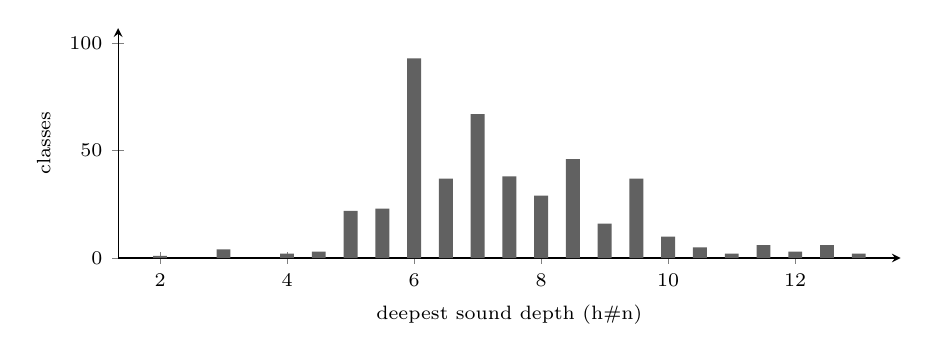
\begin{tikzpicture}
\begin{axis}[
  width=0.95\linewidth, height=45mm,
  ybar, bar width=5pt,
  xlabel={deepest sound depth (h\#n)}, ylabel={classes},
  ylabel near ticks, xlabel near ticks,
  ymin=0, ymax=107,
  tick label style={font=\scriptsize},
  label style={font=\scriptsize},
  axis lines=left, enlarge x limits=0.06,
]
\addplot[fill=black!62,draw=none] coordinates {(2.0,1) (3.0,4) (4.0,2) (4.5,3) (5.0,22) (5.5,23) (6.0,93) (6.5,37) (7.0,67) (7.5,38) (8.0,29) (8.5,46) (9.0,16) (9.5,37) (10.0,10) (10.5,5) (11.0,2) (11.5,6) (12.0,3) (12.5,6) (13.0,2)};
\end{axis}
\end{tikzpicture}
\end{center}

\section{The gap to the class maximum}

How much depth uniqueness costs: the class's longest helpmate minus
its deepest sound one, in plies. It is never zero.
\begin{center}
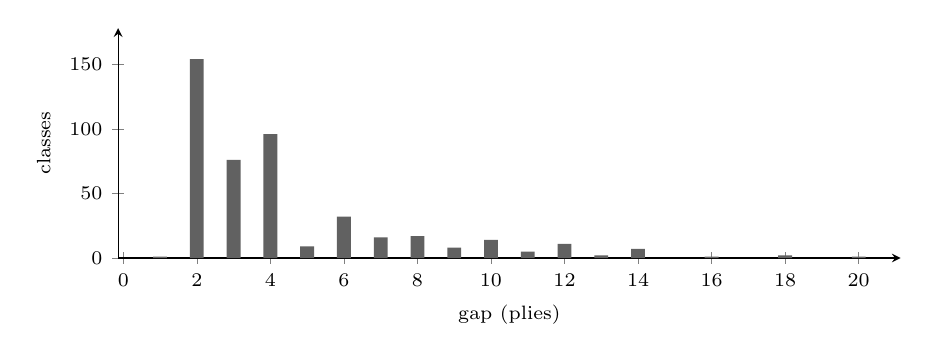
\begin{tikzpicture}
\begin{axis}[
  width=0.95\linewidth, height=45mm,
  ybar, bar width=5pt,
  xlabel={gap (plies)}, ylabel={classes},
  ylabel near ticks, xlabel near ticks,
  ymin=0, ymax=178,
  tick label style={font=\scriptsize},
  label style={font=\scriptsize},
  axis lines=left, enlarge x limits=0.06,
]
\addplot[fill=black!62,draw=none] coordinates {(1,1) (2,154) (3,76) (4,96) (5,9) (6,32) (7,16) (8,17) (9,8) (10,14) (11,5) (12,11) (13,2) (14,7) (16,1) (18,2) (20,1)};
\end{axis}
\end{tikzpicture}
\end{center}

Mean 4.4 plies, median 3,
worst 20 --- KRBvkp, which runs to
h\#16 but whose deepest sound
problem is only h\#6
(page~\pageref{hm:KRBvkp}).

\section{The ten deepest}

\begin{center}
\begin{tabular}{lrrrr}
\toprule
material & sound & class max & gap & positions \\
\midrule
KBvkbbp & h\#13 & h\#16.5 & 7 & 2 \\
KBvkrp & h\#13 & h\#16.5 & 7 & 2 \\
KBvkqbp & h\#12.5 & h\#16.5 & 8 & 59 \\
KBvkqqp & h\#12.5 & h\#17.5 & 10 & 210 \\
KBvkqrp & h\#12.5 & h\#16.5 & 8 & 495 \\
KBvkrpp & h\#12.5 & h\#16.5 & 8 & 14 \\
KBvkrrp & h\#12.5 & h\#16.5 & 8 & 79 \\
KPvkbpp & h\#12.5 & h\#15.5 & 6 & 7 \\
KBvkqp & h\#12 & h\#17 & 10 & 3 \\
KBvkrbp & h\#12 & h\#16.5 & 9 & 6 \\
\bottomrule
\end{tabular}
\end{center}

\section{Rarity}

At its deepest sound depth a class may hold a single position and
nothing else. 41 classes are like that, and
190 hold ten or fewer. Those are the positions with no
margin at all: change one man and the problem is gone.

\begin{center}
\begin{tabular}{llll}
\toprule
\multicolumn{4}{c}{classes with exactly one position at their deepest sound depth} \\
\midrule
KBBvkrp~h\#11 & KBvkppp~h\#11 & KBPvkp~h\#10.5 & KBvkbnp~h\#10.5 \\
KBvknpp~h\#10.5 & KRBvkbp~h\#10 & KRBvknp~h\#10 & KNvkqb~h\#9.5 \\
KNvkqrb~h\#9.5 & KNvkrpp~h\#9.5 & KPvknnp~h\#9.5 & KBBvkp~h\#9 \\
KNvknp~h\#8.5 & KNvkrn~h\#8.5 & KNvkrnn~h\#8.5 & KPvkqn~h\#8.5 \\
KPvkqrn~h\#8.5 & KNvkqrr~h\#8 & KBNvkq~h\#7.5 & KBvkrrb~h\#7.5 \\
KPPvkb~h\#7.5 & KPPvkn~h\#7.5 & KPPvkq~h\#7.5 & KPvkr~h\#7.5 \\
KBBNvk~h\#7 & KNNvkq~h\#7 & KNNvkr~h\#7 & KQBBvk~h\#7 \\
KRBBvk~h\#7 & KRBvkrb~h\#7 & KRvkqbn~h\#7 & KRvkqnn~h\#7 \\
KRvkqnp~h\#7 & KRvkrpp~h\#7 & KBBvk~h\#6.5 & KRvknnn~h\#6.5 \\
KRvkqb~h\#6.5 & KQvkbn~h\#6 & KRRvkr~h\#6 & KQvkqrr~h\#5 \\
KRvk~h\#4.5 &  &  &  \\
\bottomrule
\end{tabular}
\end{center}

\chapter{Three men}
\markboth{Three men}{}

3 of the 5 material classes
with 3 men that can hold a mate, deepest sound problem first.

\hmentry{No.~1\quad KPvk}{KPvk}{6k1/8/8/8/8/8/4P3/2K5 w - - 0 1}{h\#6.5}{\textbf{h\#6.5}, unique solution.\\[0.3em]The class runs to h\#8.5, so the deepest sound problem is 4~plies shallower. Every position at that depth has a saturated solution count (255 or more).\\[0.3em]13 positions of the 86\,688 indexed have a unique solution at h\#6.5.\\[0.3em]\textit{Published:} Niemann, John -- Schachmatt, No. 427, 13/07/1947; Catalogue h\# (CHM) avec 6 pieces, No. 61, 1995; Wenigsteiner im Hilfsmatt, No. 77, 1977; Problemista, No. 1569, 07-10/1981, as h\#6 (P0530828); Ban, Jenö -- Magyar Sakkelet, 1961; Ideal-Mate Encyclopedia Vol.1, No. 12, 1999, as h\#7 0.1... (P1100755)}{1...e3 2.Kf7 e4 3.Ke6 e5 4.Kd5 e6 5.Kc4 e7 6.Kb3 e8=Q 7.Ka2 Qa4\#}{https://helpman.komtera.lt/?fen=6k1/8/8/8/8/8/4P3/2K5&moves=6.5}{2 + 1}{set-play, pure, model, ideal, mirror, promotion, excelsior, excelsior:white, single-piece, single-piece:white, single-piece:black, nocapture, nocheck, umnov, promotions:q}
\hmentry{No.~1b\quad KPvk}{KPvk-b}{8/8/8/1K6/8/3P4/7k/8 w - - 0 1}{h\#6.5}{\textbf{h\#6.5}, unique solution.\\[0.3em]Same material and stipulation as No.~1, which is published; this position is not in the published database, under any mirroring.}{1...d4 2.Kg3 d5 3.Kf4 d6 4.Ke5 d7 5.Kd6 Ka5 6.Kc7 Ka6 7.Kb8 d8=Q\#}{https://helpman.komtera.lt/?fen=8/8/8/1K6/8/3P4/7k/8&moves=6.5}{2 + 1}{pure, model, ideal, mirror, promotion, single-piece, single-piece:black, nocapture, nocheck, umnov, promotions:q}
\hmentry{No.~2\quad KQvk}{KQvk}{8/8/7k/6Q1/8/8/8/K7 b - - 0 1}{h\#6}{\textbf{h\#6}, unique solution.\\[0.3em]The class runs to h\#7, so the deepest sound problem is 2~plies shallower. Every position at that depth has a saturated solution count (255 or more).\\[0.3em]3 positions of the 29\,568 indexed have a unique solution at h\#6.\\[0.3em]\textit{Published:} Csaszar, Imre -- Magyar Sakkvilag, 1945; Ideal-Mate Review, 1990; Catalogue h\# (CHM) avec 6 pieces, No. 165, 1995, as h\#6 (P0551296)\\[0.3em]\textit{Note:} the side to move is in check in the diagram.}{1.Kh7 Kb2 2.Kh8 Kc3 3.Kh7 Kd4 4.Kh8 Ke5 5.Kh7 Kf6 6.Kh8 Qg7\#}{https://helpman.komtera.lt/?fen=8/8/7k/6Q1/8/8/8/K7&moves=6}{2 + 1}{pure, model, ideal, switchback, single-piece, single-piece:black, nocapture, nocheck}
\hmentry{No.~2b\quad KQvk}{KQvk-b}{8/7k/8/6Q1/8/8/8/K7 b - - 0 1}{h\#6}{\textbf{h\#6}, unique solution.\\[0.3em]Same material and stipulation as No.~2, which is published; this position is not in the published database, under any mirroring.}{1.Kh8 Kb2 2.Kh7 Kc3 3.Kh8 Kd4 4.Kh7 Ke5 5.Kh8 Kf6 6.Kh7 Qg7\#}{https://helpman.komtera.lt/?fen=8/7k/8/6Q1/8/8/8/K7&moves=6}{2 + 1}{set-play, switchback, single-piece, single-piece:black, pendulum, nocapture, nocheck}
\hmentry{No.~3\quad KRvk}{KRvk}{4k3/8/8/8/8/8/2R5/1K6 w - - 0 1}{h\#4.5}{\textbf{h\#4.5}, unique solution.\\[0.3em]The class runs to h\#7, so the deepest sound problem is 5~plies shallower. Every position at that depth has a saturated solution count (255 or more).\\[0.3em]1 position of the 29\,568 indexed has a unique solution at h\#4.5.\\[0.3em]\textit{Published:} Ban, Jenö -- Diagramme und Figuren, No. 1295, 27/11/1965; Catalogue h\# (CHM) avec 6 pieces, No. 122, 1995; Ideal-Mate Encyclopedia Vol.1, No. 1848, 1999, as h\#5 0.1... (P0531991)}{1...Kc1 2.Kf7 Kd2 3.Kg6 Ke3 4.Kh5 Kf4 5.Kh4 Rh2\#}{https://helpman.komtera.lt/?fen=4k3/8/8/8/8/8/2R5/1K6&moves=4.5}{2 + 1}{pure, model, ideal, mirror, single-piece, single-piece:black, nocapture, nocheck}

\chapter{Four men}
\markboth{Four men}{}

37 of the 40 material classes
with 4 men that can hold a mate, deepest sound problem first.

\hmentry{No.~4\quad KPvkp}{KPvkp}{8/8/p7/8/P7/8/3K4/7k w - - 0 1}{h\#8.5}{\textbf{h\#8.5}, unique solution.\\[0.3em]The class runs to h\#14.5, so the deepest sound problem is 12~plies shallower. Every position at that depth has a saturated solution count (255 or more).\\[0.3em]2 positions of the 4\,161\,024 indexed have a unique solution at h\#8.5.}{1...Kc3 2.Kg2 Kb4 3.a5+ Kxa5 4.Kf3 Kb4 5.Ke4 a5 6.Kd5 a6 7.Kc6 a7 8.Kb7 Kc5 9.Ka6 a8=Q\#}{https://helpman.komtera.lt/?fen=8/8/p7/8/P7/8/3K4/7k&moves=8.5}{2 + 2}{pure, model, ideal, mirror, promotion, switchback, promotions:q}
\hmentry{No.~5\quad KBvkn}{KBvkn}{8/8/8/8/8/1k6/5n2/1K5B b - - 0 1}{h\#8}{\textbf{h\#8}, unique solution.\\[0.3em]The class runs to h\#12, so the deepest sound problem is 8~plies shallower. Every position at that depth has a saturated solution count (255 or more).\\[0.3em]19 positions of the 1\,892\,352 indexed have a unique solution at h\#8.}{1.Kc3 Bg2 2.Kd2 Bf1 3.Ke1 Kc2 4.Nh3 Kd3 5.Kf2 Ke4 6.Kg1 Kf3 7.Kh1 Kg3 8.Ng1 Bg2\#}{https://helpman.komtera.lt/?fen=8/8/8/8/8/1k6/5n2/1K5B&moves=8}{2 + 2}{pure, model, ideal, switchback, self-block, nocapture, nocheck}
\hmentry{No.~6\quad KBvkp}{KBvkp}{8/8/8/4k3/2p5/8/8/K3B3 b - - 0 1}{h\#8}{\textbf{h\#8}, unique solution.\\[0.3em]The class runs to h\#16, so the deepest sound problem is 16~plies shallower. Every position at that depth has a saturated solution count (255 or more).\\[0.3em]16 positions of the 5\,548\,032 indexed have a unique solution at h\#8.}{1.c3 Bh4 2.c2 Kb2 3.c1=N Kc2 4.Kd4 Kd1 5.Kc3 Be7 6.Kb2 Ba3+ 7.Ka1 Kc2 8.Na2 Bb2\#}{https://helpman.komtera.lt/?fen=8/8/8/4k3/2p5/8/8/K3B3&moves=8}{2 + 2}{pure, model, ideal, promotion, underpromotion, switchback, self-block, nocapture, umnov, promotions:n}
\hmentry{No.~7\quad KNvkb}{KNvkb}{8/8/7k/8/8/1b6/4N3/K7 b - - 0 1}{h\#8}{\textbf{h\#8}, unique solution.\\[0.3em]The class runs to h\#10.5, so the deepest sound problem is 5~plies shallower. Every position at that depth has a saturated solution count (255 or more).\\[0.3em]5 positions of the 1\,892\,352 indexed have a unique solution at h\#8.}{1.Kg5 Nd4 2.Kf4 Kb2 3.Ke3 Ka3 4.Kd2 Kb4 5.Kc1 Kc3 6.Kb1 Kd2 7.Ka1 Kc1 8.Ba2 Nc2\#}{https://helpman.komtera.lt/?fen=8/8/7k/8/8/1b6/4N3/K7&moves=8}{2 + 2}{pure, model, ideal, self-block, nocapture, nocheck}
\hmentry{No.~8\quad KNvkp}{KNvkp}{8/8/3p4/8/8/1k6/N7/K7 b - - 0 1}{h\#8}{\textbf{h\#8}, unique solution.\\[0.3em]The class runs to h\#11.5, so the deepest sound problem is 7~plies shallower. Every position at that depth has a saturated solution count (255 or more).\\[0.3em]4 positions of the 5\,548\,032 indexed have a unique solution at h\#8.}{1.d5 Kb1 2.d4 Kc1 3.d3 Kd2 4.Kb2 Nb4 5.Ka1 Kc3 6.d2 Kb3 7.d1=R Ka3 8.Rb1 Nc2\#}{https://helpman.komtera.lt/?fen=8/8/3p4/8/8/1k6/N7/K7&moves=8}{2 + 2}{pure, model, ideal, promotion, underpromotion, self-block, nocapture, nocheck, umnov, promotions:r}
\hmentry{No.~9\quad KNvkr}{KNvkr}{8/8/8/8/8/7k/5r1N/K7 b - - 0 1}{h\#8}{\textbf{h\#8}, unique solution.\\[0.3em]The class runs to h\#9.5, so the deepest sound problem is 3~plies shallower. Every position at that depth has a saturated solution count (255 or more).\\[0.3em]9 positions of the 1\,892\,352 indexed have a unique solution at h\#8.\\[0.3em]\textit{Published:} Elkies, Noam D. -- Variantim, No. 546, 11/1995, as h\#8 (P0543062); Mertes, Helmut -- feenschach, 01/1977; Ideal-Mate Encyclopedia Vol.1, No. 400, 1999, as h\#8 (P0543063)}{1.Kg2 Nf3 2.Kf1 Kb1 3.Ke2 Kb2 4.Kd3+ Kc1 5.Kc3 Kd1 6.Kb2 Nd4 7.Ka1 Kc1 8.Ra2 Nb3\#}{https://helpman.komtera.lt/?fen=8/8/8/8/8/7k/5r1N/K7&moves=8}{2 + 2}{pure, model, ideal, switchback, self-block, nocapture}
\hmentry{No.~9b\quad KNvkr}{KNvkr-b}{8/7k/N7/8/8/8/4r3/1K6 b - - 0 1}{h\#8}{\textbf{h\#8}, unique solution.\\[0.3em]Same material and stipulation as No.~9, which is published; this position is not in the published database, under any mirroring.}{1.Kg6 Nb4 2.Kf5 Nc2 3.Ke4 Kb2 4.Kd3 Kc1 5.Kc3 Kd1 6.Kb2 Nd4 7.Ka1 Kc1 8.Ra2 Nb3\#}{https://helpman.komtera.lt/?fen=8/7k/N7/8/8/8/4r3/1K6&moves=8}{2 + 2}{pure, model, ideal, switchback, self-block, nocapture, nocheck}
\hmentry{No.~10\quad KNvkn}{KNvkn}{5n2/8/8/8/8/8/3k2N1/K7 w - - 0 1}{h\#7.5}{\textbf{h\#7.5}, unique solution.\\[0.3em]The class runs to h\#10, so the deepest sound problem is 5~plies shallower. Every position at that depth has a saturated solution count (255 or more).\\[0.3em]14 positions of the 1\,892\,352 indexed have a unique solution at h\#7.5.\\[0.3em]\textit{Published:} Kotesovec, Vaclav -- Sachova skladba, No. 1065, 06/1987, as h\#8 0.1... (P0542897); ?, ? -- ?, 03/1975, as h\#8 0.1... (P0542908)}{1...Nh4 2.Ke3 Kb2 3.Kf4 Kc3 4.Kg5 Kd4 5.Kh6 Ke5 6.Kh7 Kf6 7.Kh8 Kf7 8.Nh7 Ng6\#}{https://helpman.komtera.lt/?fen=5n2/8/8/8/8/8/3k2N1/K7&moves=7.5}{2 + 2}{pure, model, ideal, self-block, nocapture, nocheck}
\hmentry{No.~10b\quad KNvkn}{KNvkn-b}{5n2/8/8/8/6N1/8/3k4/1K6 w - - 0 1}{h\#7.5}{\textbf{h\#7.5}, unique solution.\\[0.3em]Same material and stipulation as No.~10, which is published; this position is not in the published database, under any mirroring.}{1...Ne5 2.Ke3 Kc2 3.Kf4 Kd3 4.Kg5 Ke4 5.Kh6 Kf5 6.Kh7 Kf6 7.Kh8 Kf7 8.Nh7 Ng6\#}{https://helpman.komtera.lt/?fen=5n2/8/8/8/6N1/8/3k4/1K6&moves=7.5}{2 + 2}{pure, model, ideal, self-block, nocapture, nocheck}
\hmentry{No.~11\quad KPvkb}{KPvkb}{8/8/1K6/8/2b5/2P5/7k/8 w - - 0 1}{h\#7.5}{\textbf{h\#7.5}, unique solution.\\[0.3em]The class runs to h\#8.5, so the deepest sound problem is 2~plies shallower. Every position at that depth has a saturated solution count (255 or more).\\[0.3em]13 positions of the 5\,548\,032 indexed have a unique solution at h\#7.5.}{1...Ka5 2.Bd5 c4 3.Kg3 cxd5 4.Kf4 d6 5.Ke5 d7 6.Kd6 Kb5 7.Kc7 Ka6 8.Kb8 d8=Q\#}{https://helpman.komtera.lt/?fen=8/8/1K6/8/2b5/2P5/7k/8&moves=7.5}{2 + 2}{set-play, pure, model, ideal, mirror, promotion, nocheck, umnov, promotions:q}
\hmentry{No.~12\quad KPvkn}{KPvkn}{K7/8/8/n7/2P5/8/8/7k w - - 0 1}{h\#7.5}{\textbf{h\#7.5}, unique solution.\\[0.3em]The class runs to h\#8.5, so the deepest sound problem is 2~plies shallower. Every position at that depth has a saturated solution count (255 or more).\\[0.3em]8 positions of the 5\,548\,032 indexed have a unique solution at h\#7.5.}{1...c5 2.Kg2 c6 3.Kf3 c7 4.Ke4 c8=Q 5.Kd5 Qf5+ 6.Kc6 Kb8 7.Kb6 Kc8 8.Ka7 Qxa5\#}{https://helpman.komtera.lt/?fen=K7/8/8/n7/2P5/8/8/7k&moves=7.5}{2 + 2}{pure, model, ideal, mirror, promotion, single-piece, single-piece:black, promotions:q}
\hmentry{No.~13\quad KPvkq}{KPvkq}{8/K7/8/8/8/8/3P4/2q4k w - - 0 1}{h\#7.5}{\textbf{h\#7.5}, unique solution.\\[0.3em]The class runs to h\#9, so the deepest sound problem is 3~plies shallower. Every position at that depth has a saturated solution count (255 or more).\\[0.3em]32 positions of the 5\,548\,032 indexed have a unique solution at h\#7.5.}{1...d4 2.Kg2 d5 3.Kf3 d6 4.Ke4 d7 5.Kd5 d8=Q+ 6.Kc6 Qd5+ 7.Kc7 Ka6 8.Kb8 Qb7\#}{https://helpman.komtera.lt/?fen=8/K7/8/8/8/8/3P4/2q4k&moves=7.5}{2 + 2}{promotion, excelsior, excelsior:white, closed-walk, single-piece, single-piece:black, nocapture, umnov, promotions:q}
\hmentry{No.~14\quad KPvkr}{KPvkr}{8/7k/8/8/8/7r/1K5P/8 w - - 0 1}{h\#7.5}{\textbf{h\#7.5}, unique solution.\\[0.3em]The class runs to h\#8.5, so the deepest sound problem is 2~plies shallower. Every position at that depth has a saturated solution count (255 or more).\\[0.3em]1 position of the 5\,548\,032 indexed has a unique solution at h\#7.5.\\[0.3em]\textit{Published:} Maslar, Zdravko -- ?,, as h\#8 0.1... (P0542623)}{1...Ka2 2.Ra3+ Kxa3 3.Kg6 h4 4.Kf5 h5 5.Ke4 h6 6.Kd3 h7 7.Kc2 h8=Q 8.Kb1 Qb2\#}{https://helpman.komtera.lt/?fen=8/7k/8/8/8/7r/1K5P/8&moves=7.5}{2 + 2}{set-play, promotion, excelsior, excelsior:white, promotions:q}
\hmentry{No.~15\quad KBPvk}{KBPvk}{7k/8/8/8/B7/8/P7/3K4 b - - 0 1}{h\#7}{\textbf{h\#7}, unique solution.\\[0.3em]The class runs to h\#8, so the deepest sound problem is 2~plies shallower. Every position at that depth has a saturated solution count (255 or more).\\[0.3em]12 positions of the 5\,548\,032 indexed have a unique solution at h\#7.\\[0.3em]\textit{Published:} Elkies, Noam D. -- The Problemist, No. H2794, 07/2004, as h\#7 (P1187767)}{1.Kg7 Bb3 2.Kf6 a4 3.Ke5 a5 4.Kd4 a6 5.Kc3 a7 6.Kb2 a8=Q 7.Kb1 Qa2\#}{https://helpman.komtera.lt/?fen=7k/8/8/8/B7/8/P7/3K4&moves=7}{3 + 1}{promotion, excelsior, excelsior:white, closed-walk, single-piece, single-piece:black, nocapture, nocheck, promotions:q}
\hmentry{No.~15b\quad KBPvk}{KBPvk-b}{7k/8/8/8/B7/P7/8/3K4 b - - 0 1}{h\#7}{\textbf{h\#7}, unique solution.\\[0.3em]Same material and stipulation as No.~15, which is published; this position is not in the published database, under any mirroring.}{1.Kg7 Bb3 2.Kf6 a4 3.Ke5 a5 4.Kd4 a6 5.Kc3 a7 6.Kb2 a8=Q 7.Kb1 Qa2\#}{https://helpman.komtera.lt/?fen=7k/8/8/8/B7/P7/8/3K4&moves=7}{3 + 1}{promotion, single-piece, single-piece:black, nocapture, nocheck, promotions:q}
\hmentry{No.~16\quad KNPvk}{KNPvk}{8/8/8/8/8/N7/P7/3K3k b - - 0 1}{h\#7}{\textbf{h\#7}, unique solution.\\[0.3em]The class runs to h\#8.5, so the deepest sound problem is 3~plies shallower. Every position at that depth has a saturated solution count (255 or more).\\[0.3em]49 positions of the 5\,548\,032 indexed have a unique solution at h\#7.\\[0.3em]\textit{Published:} Elkies, Noam D. -- The Problemist, No. H2793, 07/2004, as h\#7 (P1187769)}{1.Kg2 Nc2 2.Kf3 a4 3.Ke4 a5 4.Kd3 a6 5.Kc3 a7 6.Kb2 a8=Q 7.Kb1 Qa1\#}{https://helpman.komtera.lt/?fen=8/8/8/8/8/N7/P7/3K3k&moves=7}{3 + 1}{promotion, excelsior, excelsior:white, single-piece, single-piece:black, nocapture, nocheck, promotions:q}
\hmentry{No.~16b\quad KNPvk}{KNPvk-b}{8/8/8/8/8/KN6/P7/7k b - - 0 1}{h\#7}{\textbf{h\#7}, unique solution.\\[0.3em]Same material and stipulation as No.~16, which is published; this position is not in the published database, under any mirroring.}{1.Kg2 Kb4 2.Kf3 a4 3.Ke4 a5 4.Kd5 a6 5.Kc6 a7 6.Kb7 Kc5 7.Ka6 a8=Q\#}{https://helpman.komtera.lt/?fen=8/8/8/8/8/KN6/P7/7k&moves=7}{3 + 1}{mirror, promotion, excelsior, excelsior:white, single-piece, single-piece:black, nocapture, nocheck, promotions:q}
\hmentry{No.~17\quad KPPvk}{KPPvk}{8/7k/8/8/8/6P1/K5P1/8 b - - 0 1}{h\#7}{\textbf{h\#7}, unique solution.\\[0.3em]The class runs to h\#8, so the deepest sound problem is 2~plies shallower. Every position at that depth has a saturated solution count (255 or more).\\[0.3em]2 positions of the 4\,161\,024 indexed have a unique solution at h\#7.\\[0.3em]\textit{Published:} Salazar Lopez, Francisco -- British Chess Magazine, 03/1973; Catalogue h\# (CHM) avec 6 pieces, No. 213, 1995; The Problemist, 05/2005; Problemkiste, No. G), 01/2010, as h\#7 (P0545149)}{1.Kg6 Ka3 2.Kf5 g4+ 3.Ke4 g5 4.Kd3 g6 5.Kc2 g7 6.Kb1 g8=Q 7.Ka1 Qa2\#}{https://helpman.komtera.lt/?fen=8/7k/8/8/8/6P1/K5P1/8&moves=7}{3 + 1}{promotion, single-piece, single-piece:black, nocapture, promotions:q}
\hmentry{No.~18\quad KQPvk}{KQPvk}{6Qk/8/8/8/8/8/4P3/2K5 b - - 0 1}{h\#7}{\textbf{h\#7}, unique solution.\\[0.3em]The class runs to h\#8, so the deepest sound problem is 2~plies shallower.\\[0.3em]12 positions of the 5\,548\,032 indexed have a unique solution at h\#7.\\[0.3em]\textit{Note:} the side to move is in check in the diagram; the solution begins with a capture.}{1.Kxg8 e3 2.Kf7 e4 3.Ke6 e5 4.Kd5 e6 5.Kc4 e7 6.Kb3 e8=Q 7.Ka2 Qa4\#}{https://helpman.komtera.lt/?fen=6Qk/8/8/8/8/8/4P3/2K5&moves=7}{3 + 1}{pure, model, ideal, mirror, promotion, excelsior, excelsior:white, single-piece, single-piece:white, single-piece:black, phoenix, nocheck, umnov, promotions:q}
\hmentry{No.~19\quad KBBvk}{KBBvk}{7k/8/7B/8/8/8/2B5/K7 w - - 0 1}{h\#6.5}{\textbf{h\#6.5}, unique solution.\\[0.3em]The class runs to h\#8, so the deepest sound problem is 3~plies shallower. Every position at that depth has a saturated solution count (255 or more).\\[0.3em]1 position of the 1\,892\,352 indexed has a unique solution at h\#6.5.\\[0.3em]\textit{Published:} Maslar, Zdravko -- feenschach, 01-03/1978; Catalogue h\# (CHM) avec 6 pieces, No. 899, 1995; Problemkiste, No. A1, 03/2012, as h\#7 0.1... (P0545758)}{1...Kb2 2.Kg8 Kc3 3.Kf7 Kd3 4.Kg6 Ke4 5.Kh5 Kf5 6.Kh4 Bg5+ 7.Kh5 Bd1\#}{https://helpman.komtera.lt/?fen=7k/8/7B/8/8/8/2B5/K7&moves=6.5}{3 + 1}{switchback, single-piece, single-piece:black, nocapture}
\hmentry{No.~20\quad KBvkb}{KBvkb}{8/8/6b1/8/8/6k1/3B4/K7 w - - 0 1}{h\#6.5}{\textbf{h\#6.5}, unique solution.\\[0.3em]The class runs to h\#10, so the deepest sound problem is 7~plies shallower. Every position at that depth has a saturated solution count (255 or more).\\[0.3em]8 positions of the 1\,892\,352 indexed have a unique solution at h\#6.5.}{1...Kb2 2.Kg4 Kc3 3.Kf5 Kd4 4.Kf6 Bc3 5.Kg7 Ke5 6.Kh8 Kf6 7.Bh7 Kf7\#}{https://helpman.komtera.lt/?fen=8/8/6b1/8/8/6k1/3B4/K7&moves=6.5}{2 + 2}{self-block, nocapture, nocheck}
\hmentry{No.~21\quad KNNvk}{KNNvk}{1k5N/8/8/8/8/8/7N/3K4 w - - 0 1}{h\#6.5}{\textbf{h\#6.5}, unique solution.\\[0.3em]The class runs to h\#8, so the deepest sound problem is 3~plies shallower. Every position at that depth has a saturated solution count (255 or more).\\[0.3em]9 positions of the 1\,892\,352 indexed have a unique solution at h\#6.5.\\[0.3em]\textit{Published:} Bebesi, Gyula -- Diagramme und Figuren, No. 1910, 12/12/1966; Catalogue h\# (CHM) avec 6 pieces, No. 624, 1995; Ideal-Mate Encyclopedia Vol.1, No. 930, 1999, as h\#7 0.1... (P0545484)}{1...Ke2 2.Kc7 Kf3 3.Kd6 Kg4 4.Ke5 Kh5 5.Kf4 Ng6+ 6.Kg3 Nf1+ 7.Kh3 Nf4\#}{https://helpman.komtera.lt/?fen=1k5N/8/8/8/8/8/7N/3K4&moves=6.5}{3 + 1}{pure, model, ideal, mirror, single-piece, single-piece:black, nocapture}
\hmentry{No.~21b\quad KNNvk}{KNNvk-b}{6kN/8/8/8/8/8/7N/3K4 w - - 0 1}{h\#6.5}{\textbf{h\#6.5}, unique solution.\\[0.3em]Same material and stipulation as No.~21, which is published; this position is not in the published database, under any mirroring.}{1...Ke2 2.Kg7 Kf3 3.Kf6 Kg4 4.Ke5 Kh5 5.Kf4 Ng6+ 6.Kg3 Nf1+ 7.Kh3 Nf4\#}{https://helpman.komtera.lt/?fen=6kN/8/8/8/8/8/7N/3K4&moves=6.5}{3 + 1}{pure, model, ideal, mirror, single-piece, single-piece:black, nocapture}
\hmentry{No.~22\quad KBNvk}{KBNvk}{8/6N1/8/8/8/2B5/8/K2k4 b - - 0 1}{h\#6}{\textbf{h\#6}, unique solution.\\[0.3em]The class runs to h\#8, so the deepest sound problem is 4~plies shallower. Every position at that depth has a saturated solution count (255 or more).\\[0.3em]23 positions of the 1\,892\,352 indexed have a unique solution at h\#6.}{1.Kc2 Ka2 2.Kc1 Kb3 3.Kb1 Kc4 4.Ka2 Ne6 5.Ka3 Bb4+ 6.Ka4 Nc5\#}{https://helpman.komtera.lt/?fen=8/6N1/8/8/8/2B5/8/K2k4&moves=6}{3 + 1}{set-play, single-piece, single-piece:black, nocapture}
\hmentry{No.~23\quad KQBvk}{KQBvk}{7B/7k/8/6Q1/8/8/8/K7 b - - 0 1}{h\#6}{\textbf{h\#6}, unique solution.\\[0.3em]The class runs to h\#7, so the deepest sound problem is 2~plies shallower. Every position at that depth has a saturated solution count (255 or more).\\[0.3em]3 positions of the 1\,892\,352 indexed have a unique solution at h\#6.\\[0.3em]\textit{Note:} the solution begins with a capture.}{1.Kxh8 Kb2 2.Kh7 Kc3 3.Kh8 Kd4 4.Kh7 Ke5 5.Kh8 Kf6 6.Kh7 Qg7\#}{https://helpman.komtera.lt/?fen=7B/7k/8/6Q1/8/8/8/K7&moves=6}{3 + 1}{switchback, single-piece, single-piece:black, pendulum, nocheck}
\hmentry{No.~24\quad KQNvk}{KQNvk}{7N/7k/8/6Q1/8/8/8/K7 b - - 0 1}{h\#6}{\textbf{h\#6}, unique solution.\\[0.3em]The class runs to h\#7, so the deepest sound problem is 2~plies shallower. Every position at that depth has a saturated solution count (255 or more).\\[0.3em]3 positions of the 1\,892\,352 indexed have a unique solution at h\#6.\\[0.3em]\textit{Note:} the solution begins with a capture.}{1.Kxh8 Kb2 2.Kh7 Kc3 3.Kh8 Kd4 4.Kh7 Ke5 5.Kh8 Kf6 6.Kh7 Qg7\#}{https://helpman.komtera.lt/?fen=7N/7k/8/6Q1/8/8/8/K7&moves=6}{3 + 1}{switchback, single-piece, single-piece:black, pendulum, nocheck}
\hmentry{No.~25\quad KQQvk}{KQQvk}{7Q/7k/8/6Q1/8/8/8/K7 b - - 0 1}{h\#6}{\textbf{h\#6}, unique solution.\\[0.3em]The class runs to h\#7, so the deepest sound problem is 2~plies shallower. Every position at that depth has a saturated solution count (255 or more).\\[0.3em]2 positions of the 1\,892\,352 indexed have a unique solution at h\#6.\\[0.3em]\textit{Note:} the side to move is in check in the diagram; the solution begins with a capture.}{1.Kxh8 Kb2 2.Kh7 Kc3 3.Kh8 Kd4 4.Kh7 Ke5 5.Kh8 Kf6 6.Kh7 Qg7\#}{https://helpman.komtera.lt/?fen=7Q/7k/8/6Q1/8/8/8/K7&moves=6}{3 + 1}{switchback, single-piece, single-piece:black, pendulum, nocheck}
\hmentry{No.~26\quad KQRvk}{KQRvk}{7R/7k/8/6Q1/8/8/8/K7 b - - 0 1}{h\#6}{\textbf{h\#6}, unique solution.\\[0.3em]The class runs to h\#7, so the deepest sound problem is 2~plies shallower. Every position at that depth has a saturated solution count (255 or more).\\[0.3em]2 positions of the 1\,892\,352 indexed have a unique solution at h\#6.\\[0.3em]\textit{Note:} the side to move is in check in the diagram; the solution begins with a capture.}{1.Kxh8 Kb2 2.Kh7 Kc3 3.Kh8 Kd4 4.Kh7 Ke5 5.Kh8 Kf6 6.Kh7 Qg7\#}{https://helpman.komtera.lt/?fen=7R/7k/8/6Q1/8/8/8/K7&moves=6}{3 + 1}{switchback, single-piece, single-piece:black, pendulum, nocheck}
\hmentry{No.~27\quad KQvkn}{KQvkn}{7k/8/8/6Q1/8/8/1n6/K7 b - - 0 1}{h\#6}{\textbf{h\#6}, unique solution.\\[0.3em]The class runs to h\#7, so the deepest sound problem is 2~plies shallower. Every position at that depth has a saturated solution count (255 or more).\\[0.3em]4 positions of the 1\,892\,352 indexed have a unique solution at h\#6.}{1.Kh7 Kxb2 2.Kh8 Kc3 3.Kh7 Kd4 4.Kh8 Ke5 5.Kh7 Kf6 6.Kh8 Qg7\#}{https://helpman.komtera.lt/?fen=7k/8/8/6Q1/8/8/1n6/K7&moves=6}{2 + 2}{set-play, pure, model, ideal, switchback, single-piece, single-piece:black, pendulum, nocheck}
\hmentry{No.~28\quad KQvkp}{KQvkp}{K7/1p6/8/8/8/8/4Q3/5k2 b - - 0 1}{h\#6}{\textbf{h\#6}, unique solution.\\[0.3em]The class runs to h\#7, so the deepest sound problem is 2~plies shallower. Every position at that depth has a saturated solution count (255 or more).\\[0.3em]4 positions of the 5\,548\,032 indexed have a unique solution at h\#6.\\[0.3em]\textit{Note:} the side to move is in check in the diagram.}{1.Kg1 Kxb7 2.Kh1 Kc6 3.Kg1 Kd5 4.Kh1 Ke4 5.Kg1 Kf3 6.Kh1 Qg2\#}{https://helpman.komtera.lt/?fen=K7/1p6/8/8/8/8/4Q3/5k2&moves=6}{2 + 2}{pure, model, ideal, switchback, single-piece, single-piece:black, nocheck}
\hmentry{No.~29\quad KRBvk}{KRBvk}{6R1/8/7k/8/8/8/8/K2B4 b - - 0 1}{h\#6}{\textbf{h\#6}, unique solution.\\[0.3em]The class runs to h\#7, so the deepest sound problem is 2~plies shallower.\\[0.3em]20 positions of the 1\,892\,352 indexed have a unique solution at h\#6.}{1.Kh7 Kb2 2.Kh6 Kc3 3.Kh7 Kd4 4.Kh6 Ke5 5.Kh7 Kf6 6.Kh6 Rh8\#}{https://helpman.komtera.lt/?fen=6R1/8/7k/8/8/8/8/K2B4&moves=6}{3 + 1}{set-play, mirror, switchback, single-piece, single-piece:black, pendulum, nocapture, nocheck}
\hmentry{No.~30\quad KRPvk}{KRPvk}{8/7k/6R1/8/8/8/P7/K7 b - - 0 1}{h\#6}{\textbf{h\#6}, unique solution.\\[0.3em]The class runs to h\#8, so the deepest sound problem is 4~plies shallower. Every position at that depth has a saturated solution count (255 or more).\\[0.3em]25 positions of the 5\,548\,032 indexed have a unique solution at h\#6.}{1.Kh8 a4 2.Kh7 a5 3.Kh8 a6 4.Kh7 a7 5.Kh8 a8=Q+ 6.Kh7 Qg8\#}{https://helpman.komtera.lt/?fen=8/7k/6R1/8/8/8/P7/K7&moves=6}{3 + 1}{promotion, excelsior, excelsior:white, switchback, single-piece, single-piece:white, single-piece:black, pendulum, nocapture, promotions:q}
\hmentry{No.~31\quad KRvkp}{KRvkp}{8/8/7k/6R1/8/1p6/8/K7 b - - 0 1}{h\#6}{\textbf{h\#6}, unique solution.\\[0.3em]The class runs to h\#7, so the deepest sound problem is 2~plies shallower. Every position at that depth has a saturated solution count (255 or more).\\[0.3em]84 positions of the 5\,548\,032 indexed have a unique solution at h\#6.}{1.Kh7 Kb2 2.Kh8 Kc3 3.b2 Kd4 4.b1=R Ke5 5.Rb8 Kf6 6.Rg8 Rh5\#}{https://helpman.komtera.lt/?fen=8/8/7k/6R1/8/1p6/8/K7&moves=6}{2 + 2}{set-play, pure, model, ideal, promotion, underpromotion, self-block, nocapture, nocheck, umnov, promotions:r}
\hmentry{No.~32\quad KQvkq}{KQvkq}{8/8/5k2/8/6Q1/q7/8/K7 w - - 0 1}{h\#5.5}{\textbf{h\#5.5}, unique solution.\\[0.3em]The class runs to h\#7, so the deepest sound problem is 3~plies shallower. Every position at that depth has a saturated solution count (255 or more).\\[0.3em]7 positions of the 1\,892\,352 indexed have a unique solution at h\#5.5.\\[0.3em]\textit{Published:} Sheglow, Wiktor S. -- Suomen Tehtäväniekat, No. (257), 05-06/1998, as h\#6 0.1... (P0574108)\\[0.3em]\textit{Note:} the side to move is in check in the diagram.}{1...Kb1 2.Qd3+ Kc1 3.Qg6 Kd2 4.Kg7 Ke3 5.Kh6 Kf4 6.Qh7 Qg5\#}{https://helpman.komtera.lt/?fen=8/8/5k2/8/6Q1/q7/8/K7&moves=5.5}{2 + 2}{pure, model, ideal, self-block, nocapture}
\hmentry{No.~32b\quad KQvkq}{KQvkq-b}{8/7k/8/6Q1/8/8/1q6/K7 w - - 0 1}{h\#5.5}{\textbf{h\#5.5}, unique solution.\\[0.3em]Same material and stipulation as No.~32, which is published; this position is not in the published database, under any mirroring.\\[0.3em]\textit{Note:} the side to move is in check in the diagram; the solution begins with a capture.}{1...Kxb2 2.Kh8 Kc3 3.Kh7 Kd4 4.Kh8 Ke5 5.Kh7 Kf6 6.Kh8 Qg7\#}{https://helpman.komtera.lt/?fen=8/7k/8/6Q1/8/8/1q6/K7&moves=5.5}{2 + 2}{pure, model, ideal, switchback, single-piece, single-piece:black, pendulum, nocheck}
\hmentry{No.~33\quad KRvkq}{KRvkq}{8/8/5k2/8/8/6R1/5q2/K7 w - - 0 1}{h\#5.5}{\textbf{h\#5.5}, unique solution.\\[0.3em]The class runs to h\#7.5, so the deepest sound problem is 4~plies shallower. Every position at that depth has a saturated solution count (255 or more).\\[0.3em]6 positions of the 1\,892\,352 indexed have a unique solution at h\#5.5.}{1...Kb1 2.Qf5+ Kc1 3.Qg6 Kd2 4.Kg7 Ke3 5.Kh6 Kf4 6.Kh5 Rh3\#}{https://helpman.komtera.lt/?fen=8/8/5k2/8/8/6R1/5q2/K7&moves=5.5}{2 + 2}{pure, model, ideal, self-block, nocapture}
\hmentry{No.~34\quad KRvkr}{KRvkr}{8/8/5k2/8/6R1/8/7r/K7 w - - 0 1}{h\#5.5}{\textbf{h\#5.5}, unique solution.\\[0.3em]The class runs to h\#7, so the deepest sound problem is 3~plies shallower. Every position at that depth has a saturated solution count (255 or more).\\[0.3em]9 positions of the 1\,892\,352 indexed have a unique solution at h\#5.5.}{1...Kb1 2.Rh6 Kc2 3.Rg6 Kd3 4.Kg7 Ke4 5.Kh6 Kf5 6.Rg7 Rh4\#}{https://helpman.komtera.lt/?fen=8/8/5k2/8/6R1/8/7r/K7&moves=5.5}{2 + 2}{pure, model, ideal, self-block, nocapture, nocheck}
\hmentry{No.~35\quad KQvkb}{KQvkb}{8/8/7k/8/8/b5Q1/8/K7 b - - 0 1}{h\#5}{\textbf{h\#5}, unique solution.\\[0.3em]The class runs to h\#6, so the deepest sound problem is 2~plies shallower.\\[0.3em]64 positions of the 1\,892\,352 indexed have a unique solution at h\#5.}{1.Kh5 Qxa3 2.Kg4 Qa2 3.Kf3 Kb2 4.Ke2 Kc3+ 5.Kd1 Qd2\#}{https://helpman.komtera.lt/?fen=8/8/7k/8/8/b5Q1/8/K7&moves=5}{2 + 2}{single-piece, single-piece:black}
\hmentry{No.~36\quad KQvkr}{KQvkr}{8/8/8/8/7k/1r4Q1/8/K7 b - - 0 1}{h\#5}{\textbf{h\#5}, unique solution.\\[0.3em]The class runs to h\#6, so the deepest sound problem is 2~plies shallower. Every position at that depth has a saturated solution count (255 or more).\\[0.3em]7 positions of the 1\,892\,352 indexed have a unique solution at h\#5.\\[0.3em]\textit{Note:} the side to move is in check in the diagram.}{1.Kh5 Qxb3 2.Kg4 Qa2 3.Kf3 Kb2 4.Ke2 Kc3+ 5.Kd1 Qd2\#}{https://helpman.komtera.lt/?fen=8/8/8/8/7k/1r4Q1/8/K7&moves=5}{2 + 2}{single-piece, single-piece:black}
\hmentry{No.~37\quad KRNvk}{KRNvk}{8/8/8/8/6k1/N4R2/8/K7 b - - 0 1}{h\#5}{\textbf{h\#5}, unique solution.\\[0.3em]The class runs to h\#7, so the deepest sound problem is 4~plies shallower. Every position at that depth has a saturated solution count (255 or more).\\[0.3em]19 positions of the 1\,892\,352 indexed have a unique solution at h\#5.\\[0.3em]\textit{Published:} Maslar, Zdravko -- Stern, 15/01/1981; Catalogue h\# (CHM) avec 6 pieces, No. 784, 1995, as h\#5 (P0545644)}{1.Kg5 Rb3 2.Kf4 Rb2 3.Ke3 Nc2+ 4.Kd2 Ne3+ 5.Kc1 Rc2\#}{https://helpman.komtera.lt/?fen=8/8/8/8/6k1/N4R2/8/K7&moves=5}{3 + 1}{set-play, single-piece, single-piece:black, nocapture, umnov}
\hmentry{No.~37b\quad KRNvk}{KRNvk-b}{8/8/8/6k1/8/N4R2/8/K7 b - - 0 1}{h\#5}{\textbf{h\#5}, unique solution.\\[0.3em]Same material and stipulation as No.~37, which is published; this position is not in the published database, under any mirroring.}{1.Kg4 Rb3 2.Kf4 Rb2 3.Ke3 Nc2+ 4.Kd2 Ne3+ 5.Kc1 Rc2\#}{https://helpman.komtera.lt/?fen=8/8/8/6k1/8/N4R2/8/K7&moves=5}{3 + 1}{set-play, single-piece, single-piece:black, nocapture, umnov}
\hmentry{No.~38\quad KRvkb}{KRvkb}{8/8/8/8/8/7k/6R1/K4b2 b - - 0 1}{h\#5}{\textbf{h\#5}, unique solution.\\[0.3em]The class runs to h\#7, so the deepest sound problem is 4~plies shallower. Every position at that depth has a saturated solution count (255 or more).\\[0.3em]365 positions of the 1\,892\,352 indexed have a unique solution at h\#5.}{1.Bd3 Ra2 2.Kg3 Kb2 3.Kf2 Kc3+ 4.Ke1 Kxd3 5.Kd1 Ra1\#}{https://helpman.komtera.lt/?fen=8/8/8/8/8/7k/6R1/K4b2&moves=5}{2 + 2}{pure, model, ideal, mirror, indian}
\hmentry{No.~39\quad KRvkn}{KRvkn}{8/8/8/8/8/n6k/6R1/K7 b - - 0 1}{h\#5}{\textbf{h\#5}, unique solution.\\[0.3em]The class runs to h\#7, so the deepest sound problem is 4~plies shallower. Every position at that depth has a saturated solution count (255 or more).\\[0.3em]247 positions of the 1\,892\,352 indexed have a unique solution at h\#5.}{1.Nb5 Ra2 2.Kg3 Kb2 3.Kf2 Kc2 4.Ke1 Kd3 5.Kd1 Ra1\#}{https://helpman.komtera.lt/?fen=8/8/8/8/8/n6k/6R1/K7&moves=5}{2 + 2}{pure, model, mirror, nocapture, nocheck}
\hmentry{No.~40\quad KRRvk}{KRRvk}{8/8/8/8/8/8/1R6/K4kR1 b - - 0 1}{h\#4}{\textbf{h\#4}, unique solution.\\[0.3em]The class runs to h\#7, so the deepest sound problem is 6~plies shallower. Every position at that depth has a saturated solution count (255 or more).\\[0.3em]27 positions of the 1\,892\,352 indexed have a unique solution at h\#4.\\[0.3em]\textit{Note:} the side to move is in check in the diagram; the solution begins with a capture.}{1.Kxg1 Kb1 2.Kf1 Kc2 3.Ke1 Kd3 4.Kd1 Rb1\#}{https://helpman.komtera.lt/?fen=8/8/8/8/8/8/1R6/K4kR1&moves=4}{3 + 1}{pure, model, ideal, mirror, switchback, single-piece, single-piece:black, nocheck}

\chapter{Five men}
\markboth{Five men}{}

181 of the 185 material classes
with 5 men that can hold a mate, deepest sound problem first.

\hmentry{No.~41\quad KBvkrp}{KBvkrp}{K7/8/3p4/8/8/2k5/8/5Br1 b - - 0 1}{h\#13}{\textbf{h\#13}, unique solution.\\[0.3em]The class runs to h\#16.5, so the deepest sound problem is 7~plies shallower. Every position at that depth has a saturated solution count (255 or more).\\[0.3em]2 positions of the 355\,074\,048 indexed have a unique solution at h\#13.}{1.d5 Kb7 2.d4 Kc6 3.d3 Kd5 4.d2 Ke4 5.d1=N Kf3 6.Ne3 Kf2 7.Kd2 Kxg1 8.Ke1 Kh2 9.Kf2 Kh3 10.Kg1 Kg3 11.Kh1 Bh3 12.Nf1+ Kf2 13.Nh2 Bg2\#}{https://helpman.komtera.lt/?fen=K7/8/3p4/8/8/2k5/8/5Br1&moves=13}{2 + 3}{pure, model, ideal, promotion, underpromotion, closed-walk, self-block, umnov, promotions:n}
\hmentry{No.~42\quad KBvkqp}{KBvkqp}{K7/1B6/8/4q3/8/1p6/k7/8 b - - 0 1}{h\#12}{\textbf{h\#12}, unique solution.\\[0.3em]The class runs to h\#17, so the deepest sound problem is 10~plies shallower. Every position at that depth has a saturated solution count (255 or more).\\[0.3em]3 positions of the 355\,074\,048 indexed have a unique solution at h\#12.}{1.b2 Ka7 2.Kb3 Kb6 3.Kc4 Ba6+ 4.Kd5 Kb5 5.Ke4+ Kc4 6.Kf3 Kd3 7.Kg2 Kd2 8.Kh1 Be2 9.b1=N+ Ke1 10.Nd2 Kf2 11.Nf3 Bf1 12.Nh2 Bg2\#}{https://helpman.komtera.lt/?fen=K7/1B6/8/4q3/8/1p6/k7/8&moves=12}{2 + 3}{pure, model, promotion, underpromotion, self-block, nocapture, umnov, promotions:n}
\hmentry{No.~43\quad KBvkbp}{KBvkbp}{8/8/2k2p2/8/3K4/8/8/1B5b w - - 0 1}{h\#11.5}{\textbf{h\#11.5}, unique solution.\\[0.3em]The class runs to h\#16, so the deepest sound problem is 9~plies shallower. Every position at that depth has a saturated solution count (255 or more).\\[0.3em]8 positions of the 355\,074\,048 indexed have a unique solution at h\#11.5.}{1...Ke3 2.f5 Kf2 3.f4 Kg1 4.f3 Kxh1 5.f2 Kg2 6.f1=N Kf2 7.Kd5 Ba2+ 8.Ke4 Ke1 9.Kf3 Be6 10.Kg2 Bh3+ 11.Kh1 Kf2 12.Nh2 Bg2\#}{https://helpman.komtera.lt/?fen=8/8/2k2p2/8/3K4/8/8/1B5b&moves=11.5}{2 + 3}{pure, model, ideal, promotion, underpromotion, switchback, closed-walk, self-block, kniest, umnov, promotions:n}
\hmentry{No.~44\quad KBPvkp}{KBPvkp}{5B2/8/8/7p/7P/1k6/8/1K6 w - - 0 1}{h\#10.5}{\textbf{h\#10.5}, unique solution.\\[0.3em]The class runs to h\#16, so the deepest sound problem is 11~plies shallower. Every position at that depth has a saturated solution count (255 or more).\\[0.3em]1 position of the 266\,305\,536 indexed has a unique solution at h\#10.5.\\[0.3em]\textit{Published:} Szentai, Endre -- Magyar Sakkelet, 1958; Suomen Tehtäväniekat, No. 320, 18/10/1999; Ideal-Mate Encyclopedia Vol.1, No. 1304, 1999, as h\#11 0.1... (P0577820)}{1...Kc1 2.Kc4 Kd2 3.Kd5 Ke3 4.Ke6 Kf4 5.Kf7 Kg5 6.Kg8 Kxh5 7.Kh8 Kg6 8.Kg8 h5 9.Kh8 h6 10.Kg8 h7+ 11.Kh8 Bg7\#}{https://helpman.komtera.lt/?fen=5B2/8/8/7p/7P/1k6/8/1K6&moves=10.5}{3 + 2}{pure, model, ideal, switchback, single-piece, single-piece:black}
\hmentry{No.~45\quad KPvkpp}{KPvkpp}{6k1/8/8/8/1p2p3/8/4P3/K7 b - - 0 1}{h\#10}{\textbf{h\#10}, unique solution.\\[0.3em]The class runs to h\#15.5, so the deepest sound problem is 11~plies shallower. Every position at that depth has a saturated solution count (255 or more).\\[0.3em]2 positions of the 199\,729\,152 indexed have a unique solution at h\#10.\\[0.3em]\textit{Published:} Ban, Jenö -- Stella Polaris, No. 1072, 06/1967; Ideal-Mate Encyclopedia Vol.1, No. 70, 1999, as h\#10 (P0559294)}{1.b3 Kb1 2.b2 Kc2 3.b1=B+ Kc1 4.Bd3 exd3 5.Kf7 dxe4 6.Ke6 e5 7.Kd5 e6 8.Kc4 e7 9.Kb3 e8=Q 10.Ka2 Qa4\#}{https://helpman.komtera.lt/?fen=6k1/8/8/8/1p2p3/8/4P3/K7&moves=10}{2 + 3}{pure, model, ideal, mirror, promotion, underpromotion, excelsior, excelsior:white, umnov, promotions:qb}
\hmentry{No.~46\quad KBvknp}{KBvknp}{8/k1B2p2/8/5n2/8/8/K7/8 w - - 0 1}{h\#9.5}{\textbf{h\#9.5}, unique solution.\\[0.3em]The class runs to h\#15.5, so the deepest sound problem is 12~plies shallower. Every position at that depth has a saturated solution count (255 or more).\\[0.3em]2 positions of the 355\,074\,048 indexed have a unique solution at h\#9.5.}{1...Kb3 2.Kb7 Kc4 3.Kc8 Kd5 4.Kd7 Ke5 5.Ke8 Kf6 6.Kf8 Bd6+ 7.Kg8 Bf8 8.Kh8 Kxf7 9.Nh6+ Kg6 10.Ng8 Bg7\#}{https://helpman.komtera.lt/?fen=8/k1B2p2/8/5n2/8/8/K7/8&moves=9.5}{2 + 3}{pure, model, ideal, self-block, umnov}
\hmentry{No.~47\quad KBvkqn}{KBvkqn}{8/8/5q2/8/8/1k6/8/1K1n1B2 w - - 0 1}{h\#9.5}{\textbf{h\#9.5}, unique solution.\\[0.3em]The class runs to h\#13, so the deepest sound problem is 7~plies shallower. Every position at that depth has a saturated solution count (255 or more).\\[0.3em]46 positions of the 121\,110\,528 indexed have a unique solution at h\#9.5.}{1...Kc1 2.Nf2 Kd2 3.Nh3 Ke3 4.Kc2 Bd3+ 5.Kd1 Bf5 6.Ke1 Kf3 7.Kf1 Kg3 8.Kg1 Bd3 9.Kh1 Bf1 10.Ng1 Bg2\#}{https://helpman.komtera.lt/?fen=8/8/5q2/8/8/1k6/8/1K1n1B2&moves=9.5}{2 + 3}{pure, model, switchback, self-block, nocapture}
\hmentry{No.~48\quad KBvkrn}{KBvkrn}{8/8/5r2/8/8/1k6/4B3/1K1n4 w - - 0 1}{h\#9.5}{\textbf{h\#9.5}, unique solution.\\[0.3em]The class runs to h\#12.5, so the deepest sound problem is 6~plies shallower. Every position at that depth has a saturated solution count (255 or more).\\[0.3em]24 positions of the 121\,110\,528 indexed have a unique solution at h\#9.5.}{1...Kc1 2.Nf2 Kd2 3.Nh3 Ke3 4.Kc2 Bd3+ 5.Kd1 Bf5 6.Ke1 Kf3 7.Kf1 Kg3 8.Kg1 Bd3 9.Kh1 Bf1 10.Ng1 Bg2\#}{https://helpman.komtera.lt/?fen=8/8/5r2/8/8/1k6/4B3/1K1n4&moves=9.5}{2 + 3}{pure, model, switchback, self-block, nocapture}
\hmentry{No.~49\quad KNvkpp}{KNvkpp}{8/6p1/1K2k1p1/8/8/8/8/2N5 w - - 0 1}{h\#9.5}{\textbf{h\#9.5}, unique solution.\\[0.3em]The class runs to h\#11.5, so the deepest sound problem is 4~plies shallower. Every position at that depth has a saturated solution count (255 or more).\\[0.3em]2 positions of the 266\,305\,536 indexed have a unique solution at h\#9.5.}{1...Kc7 2.g5 Kd8 3.g4 Ke8 4.g3 Kf8 5.g2 Kxg7 6.g1=R+ Kh7 7.Kf7 Kh6 8.Kg8 Nd3 9.Kh8 Ne5 10.Rg8 Nf7\#}{https://helpman.komtera.lt/?fen=8/6p1/1K2k1p1/8/8/8/8/2N5&moves=9.5}{2 + 3}{pure, model, ideal, promotion, underpromotion, self-block, promotions:r}
\hmentry{No.~50\quad KNvkqb}{KNvkqb}{7k/6N1/8/8/8/8/b2q4/1K6 w - - 0 1}{h\#9.5}{\textbf{h\#9.5}, unique solution.\\[0.3em]The class runs to h\#11.5, so the deepest sound problem is 4~plies shallower. Every position at that depth has a saturated solution count (255 or more).\\[0.3em]1 position of the 121\,110\,528 indexed has a unique solution at h\#9.5.\\[0.3em]\textit{Published:} Sheglow, Wiktor S. -- Suomen Tehtäväniekat, No. (291), 05-06/1998, as h\#10 0.1... (P0574142)\\[0.3em]\textit{Note:} the side to move is in check in the diagram.}{1...Ka1 2.Kg8 Nf5 3.Kf7 Ne3 4.Ke6 Nc2 5.Kd5 Kb2 6.Kc4 Ka3 7.Kc3 Ka4 8.Kb2 Nd4 9.Ka1 Ka3 10.Bb1 Nb3\#}{https://helpman.komtera.lt/?fen=7k/6N1/8/8/8/8/b2q4/1K6&moves=9.5}{2 + 3}{pure, model, switchback, self-block, nocapture, nocheck}
\hmentry{No.~51\quad KNvkqp}{KNvkqp}{8/8/4p3/4k3/8/8/2q5/K3N3 w - - 0 1}{h\#9.5}{\textbf{h\#9.5}, unique solution.\\[0.3em]The class runs to h\#11.5, so the deepest sound problem is 4~plies shallower. Every position at that depth has a saturated solution count (255 or more).\\[0.3em]194 positions of the 355\,074\,048 indexed have a unique solution at h\#9.5.}{1...Nf3+ 2.Kf4 Nd2 3.Qd1+ Kb2 4.e5 Kc3 5.e4 Kd4 6.Kg3 Ke5 7.Kf2 Kf4 8.Ke1 Kg3 9.e3 Kg2 10.e2 Nf3\#}{https://helpman.komtera.lt/?fen=8/8/4p3/4k3/8/8/2q5/K3N3&moves=9.5}{2 + 3}{pure, model, ideal, switchback, self-block, nocapture}
\hmentry{No.~52\quad KPvkbp}{KPvkbp}{8/8/6p1/8/6P1/k7/8/Kb6 w - - 0 1}{h\#9.5}{\textbf{h\#9.5}, unique solution.\\[0.3em]The class runs to h\#14.5, so the deepest sound problem is 10~plies shallower. Every position at that depth has a saturated solution count (255 or more).\\[0.3em]9 positions of the 266\,305\,536 indexed have a unique solution at h\#9.5.\\[0.3em]\textit{Published:} Locker, Miklos S. -- Magyar Sakkelet, 02/1966, as h\#10 0.1... (P0564289)}{1...g5 2.Kb4 Kb2 3.Kc5 Kc3 4.Kd6 Kd4 5.Ke7 Ke5 6.Kf8 Kf6 7.Ba2 Kxg6 8.Kg8 Kh6 9.Kh8 g6 10.Bg8 g7\#}{https://helpman.komtera.lt/?fen=8/8/6p1/8/6P1/k7/8/Kb6&moves=9.5}{2 + 3}{pure, model, ideal, self-block, nocheck}
\hmentry{No.~52b\quad KPvkbp}{KPvkbp-b}{8/8/6p1/8/6P1/k7/2b5/K7 w - - 0 1}{h\#9.5}{\textbf{h\#9.5}, unique solution.\\[0.3em]Same material and stipulation as No.~52, which is published; this position is not in the published database, under any mirroring.}{1...g5 2.Kb4 Kb2 3.Kc5 Kc3 4.Kd6 Kd4 5.Ke7 Ke5 6.Kf8 Kf6 7.Bb3 Kxg6 8.Kg8 Kh6 9.Kh8 g6 10.Bg8 g7\#}{https://helpman.komtera.lt/?fen=8/8/6p1/8/6P1/k7/2b5/K7&moves=9.5}{2 + 3}{pure, model, ideal, self-block, nocheck}
\hmentry{No.~53\quad KBBvkn}{KBBvkn}{8/8/4n3/8/3B4/8/1B4k1/3K4 b - - 0 1}{h\#9}{\textbf{h\#9}, unique solution.\\[0.3em]The class runs to h\#12, so the deepest sound problem is 6~plies shallower. Every position at that depth has a saturated solution count (255 or more).\\[0.3em]2 positions of the 121\,110\,528 indexed have a unique solution at h\#9.}{1.Kf3 Bc1 2.Ke4 Ke2 3.Kxd4 Kf3 4.Ke5 Kg4 5.Kf6 Kh5 6.Kg7 Bh6+ 7.Kh8 Kg6 8.Nf8+ Kf7 9.Nh7 Bg7\#}{https://helpman.komtera.lt/?fen=8/8/4n3/8/3B4/8/1B4k1/3K4&moves=9}{3 + 2}{pure, model, ideal, self-block}
\hmentry{No.~54\quad KBBvkp}{KBBvkp}{3K4/1B6/2B5/8/1k6/8/5p2/8 b - - 0 1}{h\#9}{\textbf{h\#9}, unique solution.\\[0.3em]The class runs to h\#16, so the deepest sound problem is 14~plies shallower. Every position at that depth has a saturated solution count (255 or more).\\[0.3em]1 position of the 355\,074\,048 indexed has a unique solution at h\#9.}{1.Kc5 Bc8 2.Kxc6 Ke7 3.Kd5 Kf6 4.Ke4 Kg5 5.Kf3 Kh4 6.Kg2 Bh3+ 7.Kh1 Kg3 8.f1=N+ Kf2 9.Nh2 Bg2\#}{https://helpman.komtera.lt/?fen=3K4/1B6/2B5/8/1k6/8/5p2/8&moves=9}{3 + 2}{pure, model, ideal, promotion, underpromotion, self-block, umnov, promotions:n}
\hmentry{No.~55\quad KBvkbn}{KBvkbn}{8/8/1n6/3b4/8/8/8/KBk5 b - - 0 1}{h\#9}{\textbf{h\#9}, unique solution.\\[0.3em]The class runs to h\#12, so the deepest sound problem is 6~plies shallower. Every position at that depth has a saturated solution count (255 or more).\\[0.3em]57 positions of the 121\,110\,528 indexed have a unique solution at h\#9.}{1.Kd2 Bd3 2.Kc3 Ba6 3.Kb4 Kb2 4.Ka5 Kc3 5.Nc8 Kd4 6.Kb6 Kxd5 7.Ka7 Kc6 8.Ka8 Kc7 9.Na7 Bb7\#}{https://helpman.komtera.lt/?fen=8/8/1n6/3b4/8/8/8/KBk5&moves=9}{2 + 3}{pure, model, ideal, self-block, nocheck}
\hmentry{No.~56\quad KBvknn}{KBvknn}{8/8/8/8/8/8/5n2/kBK4n b - - 0 1}{h\#9}{\textbf{h\#9}, unique solution.\\[0.3em]The class runs to h\#12.5, so the deepest sound problem is 7~plies shallower. Every position at that depth has a saturated solution count (255 or more).\\[0.3em]34 positions of the 121\,110\,528 indexed have a unique solution at h\#9.}{1.Nh3 Kd2 2.Kb2 Ke3 3.Kc1 Be4 4.Kd1 Bxh1 5.Ke1 Kf3 6.Kf1 Bg2+ 7.Kg1 Bf1 8.Kh1 Kg3 9.Ng1 Bg2\#}{https://helpman.komtera.lt/?fen=8/8/8/8/8/8/5n2/kBK4n&moves=9}{2 + 3}{pure, model, ideal, switchback, self-block, kniest, umnov}
\hmentry{No.~57\quad KBvkpp}{KBvkpp}{8/6k1/8/p3p3/8/8/1B6/K7 b - - 0 1}{h\#9}{\textbf{h\#9}, unique solution.\\[0.3em]The class runs to h\#16, so the deepest sound problem is 14~plies shallower. Every position at that depth has a saturated solution count (255 or more).\\[0.3em]51 positions of the 266\,305\,536 indexed have a unique solution at h\#9.}{1.Kh8 Ba3 2.e4 Kb2 3.e3 Kc3 4.e2 Kd4 5.e1=N Ke5 6.Nf3+ Kf6 7.Ng5 Bf8 8.Nh7+ Kf7 9.a4 Bg7\#}{https://helpman.komtera.lt/?fen=8/6k1/8/p3p3/8/8/1B6/K7&moves=9}{2 + 3}{pure, model, promotion, underpromotion, self-block, nocapture, promotions:n}
\hmentry{No.~58\quad KNPvkp}{KNPvkp}{N7/8/8/8/6k1/4p3/4P3/K7 b - - 0 1}{h\#9}{\textbf{h\#9}, unique solution.\\[0.3em]The class runs to h\#14, so the deepest sound problem is 10~plies shallower. Every position at that depth has a saturated solution count (255 or more).\\[0.3em]9 positions of the 266\,305\,536 indexed have a unique solution at h\#9.}{1.Kg3 Nb6 2.Kf2 Nc4 3.Ke1 Nd2 4.exd2 e4 5.Kd1 e5 6.Kc1 e6 7.d1=R e7 8.Rd2 e8=Q 9.Rc2 Qe1\#}{https://helpman.komtera.lt/?fen=N7/8/8/8/6k1/4p3/4P3/K7&moves=9}{3 + 2}{promotion, underpromotion, excelsior, excelsior:white, switchback, self-block, nocheck, promotions:qr}
\hmentry{No.~59\quad KPvknp}{KPvknp}{6k1/8/7n/8/8/p7/P7/K7 b - - 0 1}{h\#9}{\textbf{h\#9}, unique solution.\\[0.3em]The class runs to h\#14.5, so the deepest sound problem is 11~plies shallower. Every position at that depth has a saturated solution count (255 or more).\\[0.3em]4 positions of the 266\,305\,536 indexed have a unique solution at h\#9.}{1.Nf5 Kb1 2.Nd4 Kc1 3.Nb3+ axb3 4.Kf7 b4 5.Ke6 b5 6.Kd5 b6 7.Kc4 b7 8.Kb3 b8=Q+ 9.Ka2 Qb1\#}{https://helpman.komtera.lt/?fen=6k1/8/7n/8/8/p7/P7/K7&moves=9}{2 + 3}{promotion, excelsior, excelsior:white, promotions:q}
\hmentry{No.~60\quad KNvkbb}{KNvkbb}{8/8/N7/7k/b1b5/8/8/K7 w - - 0 1}{h\#8.5}{\textbf{h\#8.5}, unique solution.\\[0.3em]The class runs to h\#10.5, so the deepest sound problem is 4~plies shallower. Every position at that depth has a saturated solution count (255 or more).\\[0.3em]69 positions of the 121\,110\,528 indexed have a unique solution at h\#8.5.}{1...Kb2 2.Kg4 Ka3 3.Kf3 Kxa4 4.Ke2 Kb4 5.Kd1 Kc3 6.Kc1 Nb4 7.Kb1 Kd2 8.Ka1 Kc1 9.Ba2 Nc2\#}{https://helpman.komtera.lt/?fen=8/8/N7/7k/b1b5/8/8/K7&moves=8.5}{2 + 3}{pure, model, ideal, self-block, nocheck}
\hmentry{No.~61\quad KNvkbp}{KNvkbp}{k7/8/8/7p/8/8/5b2/3K3N w - - 0 1}{h\#8.5}{\textbf{h\#8.5}, unique solution.\\[0.3em]The class runs to h\#10.5, so the deepest sound problem is 4~plies shallower. Every position at that depth has a saturated solution count (255 or more).\\[0.3em]12 positions of the 355\,074\,048 indexed have a unique solution at h\#8.5.}{1...Ke2 2.Kb7 Kf3 3.Kc6 Kf4 4.Kd5 Kg5 5.Ke4 Ng3+ 6.Kf3 Nxh5 7.Kg2 Kg4 8.Kh1 Kh3 9.Bg1 Ng3\#}{https://helpman.komtera.lt/?fen=k7/8/8/7p/8/8/5b2/3K3N&moves=8.5}{2 + 3}{pure, model, ideal, switchback, self-block}
\hmentry{No.~62\quad KNvknn}{KNvknn}{7k/8/8/8/8/8/8/KNn1n3 w - - 0 1}{h\#8.5}{\textbf{h\#8.5}, unique solution.\\[0.3em]The class runs to h\#9.5, so the deepest sound problem is 2~plies shallower. Every position at that depth has a saturated solution count (255 or more).\\[0.3em]3 positions of the 121\,110\,528 indexed have a unique solution at h\#8.5.}{1...Kb2 2.Kg7 Kc3 3.Kf6 Kd2 4.Ke5 Kd1 5.Kd4 Nd2 6.Kc3 Kxe1 7.Kb2 Kd1 8.Ka1 Kc2 9.Na2 Nb3\#}{https://helpman.komtera.lt/?fen=7k/8/8/8/8/8/8/KNn1n3&moves=8.5}{2 + 3}{pure, model, ideal, switchback, self-block, nocheck}
\hmentry{No.~63\quad KNvknp}{KNvknp}{N5k1/8/8/8/8/1p6/8/Kn6 w - - 0 1}{h\#8.5}{\textbf{h\#8.5}, unique solution.\\[0.3em]The class runs to h\#10, so the deepest sound problem is 3~plies shallower. Every position at that depth has a saturated solution count (255 or more).\\[0.3em]1 position of the 355\,074\,048 indexed has a unique solution at h\#8.5.\\[0.3em]\textit{Published:} Sheglow, Wiktor S. -- Suomen Tehtäväniekat, No. (286), 05-06/1998, as h\#9 0.1... (P0574137)}{1...Kb2 2.Nc3 Ka3 3.Kf7 Kb4 4.Ke6 Ka5 5.Kd5 Kb6 6.Kc4 Ka6 7.Kb4 Nb6 8.Ka3 Ka5 9.Na2 Nc4\#}{https://helpman.komtera.lt/?fen=N5k1/8/8/8/8/1p6/8/Kn6&moves=8.5}{2 + 3}{set-play, pure, model, ideal, closed-walk, self-block, nocapture, nocheck}
\hmentry{No.~64\quad KNvkqr}{KNvkqr}{8/7k/N7/8/8/8/4r3/Kq6 w - - 0 1}{h\#8.5}{\textbf{h\#8.5}, unique solution.\\[0.3em]The class runs to h\#9.5, so the deepest sound problem is 2~plies shallower. Every position at that depth has a saturated solution count (255 or more).\\[0.3em]8 positions of the 121\,110\,528 indexed have a unique solution at h\#8.5.\\[0.3em]\textit{Note:} the side to move is in check in the diagram; the solution begins with a capture.}{1...Kxb1 2.Kg6 Nb4 3.Kf5 Nc2 4.Ke4 Kb2 5.Kd3 Kc1 6.Kc3 Kd1 7.Kb2 Nd4 8.Ka1 Kc1 9.Ra2 Nb3\#}{https://helpman.komtera.lt/?fen=8/7k/N7/8/8/8/4r3/Kq6&moves=8.5}{2 + 3}{pure, model, ideal, switchback, self-block, nocheck}
\hmentry{No.~65\quad KNvkrn}{KNvkrn}{6k1/8/8/8/8/n7/4r3/1KN5 w - - 0 1}{h\#8.5}{\textbf{h\#8.5}, unique solution.\\[0.3em]The class runs to h\#10.5, so the deepest sound problem is 4~plies shallower. Every position at that depth has a saturated solution count (255 or more).\\[0.3em]1 position of the 121\,110\,528 indexed has a unique solution at h\#8.5.\\[0.3em]\textit{Note:} the side to move is in check in the diagram.}{1...Ka1 2.Kf7 Nxe2 3.Ke6 Kb2 4.Kd5 Kc1 5.Kc4 Kd2 6.Kb3 Nd4+ 7.Ka2 Kc3 8.Ka1 Kb3 9.Nb1 Nc2\#}{https://helpman.komtera.lt/?fen=6k1/8/8/8/8/n7/4r3/1KN5&moves=8.5}{2 + 3}{pure, model, ideal, self-block}
\hmentry{No.~66\quad KNvkrp}{KNvkrp}{6k1/8/8/1p6/8/8/1r6/K6N w - - 0 1}{h\#8.5}{\textbf{h\#8.5}, unique solution.\\[0.3em]The class runs to h\#11.5, so the deepest sound problem is 6~plies shallower. Every position at that depth has a saturated solution count (255 or more).\\[0.3em]46 positions of the 355\,074\,048 indexed have a unique solution at h\#8.5.}{1...Ng3 2.Rh2 Kb1 3.Rh8 Kc2 4.b4 Kd3 5.b3 Ke4 6.b2 Kf5 7.b1=R Kg6 8.Rb8 Nf5 9.Rf8 Ne7\#}{https://helpman.komtera.lt/?fen=6k1/8/8/1p6/8/8/1r6/K6N&moves=8.5}{2 + 3}{pure, model, ideal, promotion, underpromotion, self-block, nocapture, nocheck, promotions:r}
\hmentry{No.~67\quad KNvkrr}{KNvkrr}{8/7k/N7/8/8/8/4r3/Kr6 w - - 0 1}{h\#8.5}{\textbf{h\#8.5}, unique solution.\\[0.3em]The class runs to h\#9.5, so the deepest sound problem is 2~plies shallower. Every position at that depth has a saturated solution count (255 or more).\\[0.3em]5 positions of the 121\,110\,528 indexed have a unique solution at h\#8.5.\\[0.3em]\textit{Note:} the side to move is in check in the diagram; the solution begins with a capture.}{1...Kxb1 2.Kg6 Nb4 3.Kf5 Nc2 4.Ke4 Kb2 5.Kd3 Kc1 6.Kc3 Kd1 7.Kb2 Nd4 8.Ka1 Kc1 9.Ra2 Nb3\#}{https://helpman.komtera.lt/?fen=8/7k/N7/8/8/8/4r3/Kr6&moves=8.5}{2 + 3}{pure, model, ideal, switchback, self-block, nocheck}
\hmentry{No.~68\quad KPPvkp}{KPPvkp}{8/8/p7/8/P7/P7/K7/7k w - - 0 1}{h\#8.5}{\textbf{h\#8.5}, unique solution.\\[0.3em]The class runs to h\#14.5, so the deepest sound problem is 12~plies shallower. Every position at that depth has a saturated solution count (255 or more).\\[0.3em]6 positions of the 199\,729\,152 indexed have a unique solution at h\#8.5.}{1...Kb3 2.Kg2 Kb4 3.a5+ Kxa5 4.Kf3 Kb4 5.Ke4 a5 6.Kd5 a6 7.Kc6 a7 8.Kb7 Kc5 9.Ka6 a8=Q\#}{https://helpman.komtera.lt/?fen=8/8/p7/8/P7/P7/K7/7k&moves=8.5}{3 + 2}{pure, model, mirror, promotion, switchback, promotions:q}
\hmentry{No.~69\quad KPvkqn}{KPvkqn}{K7/8/8/8/8/2n5/2P5/2q4k w - - 0 1}{h\#8.5}{\textbf{h\#8.5}, unique solution.\\[0.3em]The class runs to h\#9.5, so the deepest sound problem is 2~plies shallower. Every position at that depth has a saturated solution count (255 or more).\\[0.3em]1 position of the 355\,074\,048 indexed has a unique solution at h\#8.5.}{1...Ka7 2.Nd5 c4 3.Kg2 cxd5 4.Kf3 d6 5.Ke4 d7 6.Kd5 d8=Q+ 7.Kc6 Qd5+ 8.Kc7 Ka6 9.Kb8 Qb7\#}{https://helpman.komtera.lt/?fen=K7/8/8/8/8/2n5/2P5/2q4k&moves=8.5}{2 + 3}{promotion, excelsior, excelsior:white, closed-walk, umnov, promotions:q}
\hmentry{No.~70\quad KPvkqp}{KPvkqp}{6kq/8/8/8/8/p7/P7/1K6 w - - 0 1}{h\#8.5}{\textbf{h\#8.5}, unique solution.\\[0.3em]The class runs to h\#14.5, so the deepest sound problem is 12~plies shallower. Every position at that depth has a saturated solution count (255 or more).\\[0.3em]9 positions of the 266\,305\,536 indexed have a unique solution at h\#8.5.}{1...Kc2 2.Qh3 Kc1 3.Qb3 axb3 4.Kf7 b4 5.Ke6 b5 6.Kd5 b6 7.Kc4 b7 8.Kb3 b8=Q+ 9.Ka2 Qb1\#}{https://helpman.komtera.lt/?fen=6kq/8/8/8/8/p7/P7/1K6&moves=8.5}{2 + 3}{set-play, promotion, excelsior, excelsior:white, promotions:q}
\hmentry{No.~71\quad KPvkrp}{KPvkrp}{8/8/8/8/6k1/5p2/2r2P2/K7 w - - 0 1}{h\#8.5}{\textbf{h\#8.5}, unique solution.\\[0.3em]The class runs to h\#14.5, so the deepest sound problem is 12~plies shallower. Every position at that depth has a saturated solution count (255 or more).\\[0.3em]101 positions of the 266\,305\,536 indexed have a unique solution at h\#8.5.}{1...Kb1 2.Re2 Kc1 3.Re3 fxe3 4.Kf5 e4+ 5.Ke6 e5 6.Kd5 e6 7.Kc4 e7 8.Kb3 e8=Q 9.Ka2 Qa4\#}{https://helpman.komtera.lt/?fen=8/8/8/8/6k1/5p2/2r2P2/K7&moves=8.5}{2 + 3}{pure, model, mirror, promotion, excelsior, excelsior:white, umnov, promotions:q}
\hmentry{No.~72\quad KBvkbb}{KBvkbb}{5b2/8/8/8/7B/7b/7k/K7 b - - 0 1}{h\#8}{\textbf{h\#8}, unique solution.\\[0.3em]The class runs to h\#10, so the deepest sound problem is 4~plies shallower. Every position at that depth has a saturated solution count (255 or more).\\[0.3em]8 positions of the 121\,110\,528 indexed have a unique solution at h\#8.}{1.Bf5 Kb2 2.Kh3 Kc3 3.Kg4 Kd4 4.Kh5 Ke5 5.Kh6 Kf6 6.Kh7 Kf7 7.Kh8 Kxf8 8.Bh7 Bf6\#}{https://helpman.komtera.lt/?fen=5b2/8/8/8/7B/7b/7k/K7&moves=8}{2 + 3}{self-block, nocheck}
\hmentry{No.~73\quad KNvkbn}{KNvkbn}{7k/8/8/8/8/1b6/8/Kn2N3 b - - 0 1}{h\#8}{\textbf{h\#8}, unique solution.\\[0.3em]The class runs to h\#10, so the deepest sound problem is 4~plies shallower. Every position at that depth has a saturated solution count (255 or more).\\[0.3em]5 positions of the 121\,110\,528 indexed have a unique solution at h\#8.}{1.Kg7 Kxb1 2.Kf6 Kc1 3.Ke5 Kd2 4.Kd4 Ke2 5.Kc3 Ke3 6.Kb2 Kd2 7.Ka1 Kc1 8.Ba2 Nc2\#}{https://helpman.komtera.lt/?fen=7k/8/8/8/8/1b6/8/Kn2N3&moves=8}{2 + 3}{pure, model, ideal, closed-walk, self-block, nocheck}
\hmentry{No.~74\quad KNvkqn}{KNvkqn}{8/7k/8/8/8/N7/1nq5/K7 b - - 0 1}{h\#8}{\textbf{h\#8}, unique solution.\\[0.3em]The class runs to h\#10.5, so the deepest sound problem is 5~plies shallower. Every position at that depth has a saturated solution count (255 or more).\\[0.3em]2 positions of the 121\,110\,528 indexed have a unique solution at h\#8.\\[0.3em]\textit{Published:} Sheglow, Wiktor S. -- Suomen Tehtäväniekat, No. (289), 05-06/1998, as h\#8 (P0574140)}{1.Qa4 Kb1 2.Kg6 Kc1 3.Kf5 Kd2 4.Ke4 Ke1 5.Kd3 Nb5 6.Kc2 Ke2 7.Kb1 Kd2 8.Qa1 Nc3\#}{https://helpman.komtera.lt/?fen=8/7k/8/8/8/N7/1nq5/K7&moves=8}{2 + 3}{pure, model, ideal, closed-walk, self-block, nocapture, nocheck}
\hmentry{No.~74b\quad KNvkqn}{KNvkqn-b}{8/N6k/8/8/8/8/1nq5/K7 b - - 0 1}{h\#8}{\textbf{h\#8}, unique solution.\\[0.3em]Same material and stipulation as No.~74, which is published; this position is not in the published database, under any mirroring.}{1.Qa4+ Kb1 2.Kg6 Kc1 3.Kf5 Kd2 4.Ke4 Ke1 5.Kd3 Nb5 6.Kc2 Ke2 7.Kb1 Kd2 8.Qa1 Nc3\#}{https://helpman.komtera.lt/?fen=8/N6k/8/8/8/8/1nq5/K7&moves=8}{2 + 3}{pure, model, ideal, closed-walk, self-block, nocapture}
\hmentry{No.~75\quad KQBvkn}{KQBvkn}{8/8/8/7B/8/2Q5/3k1n2/1K6 b - - 0 1}{h\#8}{\textbf{h\#8}, unique solution.\\[0.3em]The class runs to h\#12, so the deepest sound problem is 8~plies shallower. Every position at that depth has a saturated solution count (255 or more).\\[0.3em]25 positions of the 121\,110\,528 indexed have a unique solution at h\#8.\\[0.3em]\textit{Note:} the side to move is in check in the diagram; the solution begins with a capture.}{1.Kxc3 Be2 2.Kd2 Bf1 3.Ke1 Kc2 4.Nh3 Kd3 5.Kf2 Ke4 6.Kg1 Kf3 7.Kh1 Kg3 8.Ng1 Bg2\#}{https://helpman.komtera.lt/?fen=8/8/8/7B/8/2Q5/3k1n2/1K6&moves=8}{3 + 2}{pure, model, ideal, switchback, self-block, nocheck}
\hmentry{No.~76\quad KQNvkb}{KQNvkb}{8/8/8/6Qk/8/1b6/4N3/K7 b - - 0 1}{h\#8}{\textbf{h\#8}, unique solution.\\[0.3em]The class runs to h\#11, so the deepest sound problem is 6~plies shallower. Every position at that depth has a saturated solution count (255 or more).\\[0.3em]5 positions of the 121\,110\,528 indexed have a unique solution at h\#8.\\[0.3em]\textit{Note:} the side to move is in check in the diagram; the solution begins with a capture.}{1.Kxg5 Nd4 2.Kf4 Kb2 3.Ke3 Ka3 4.Kd2 Kb4 5.Kc1 Kc3 6.Kb1 Kd2 7.Ka1 Kc1 8.Ba2 Nc2\#}{https://helpman.komtera.lt/?fen=8/8/8/6Qk/8/1b6/4N3/K7&moves=8}{3 + 2}{pure, model, ideal, self-block, nocheck}
\hmentry{No.~77\quad KQNvkn}{KQNvkn}{5n2/8/8/8/8/8/3Q2N1/K1k5 b - - 0 1}{h\#8}{\textbf{h\#8}, unique solution.\\[0.3em]The class runs to h\#10, so the deepest sound problem is 4~plies shallower. Every position at that depth has a saturated solution count (255 or more).\\[0.3em]16 positions of the 121\,110\,528 indexed have a unique solution at h\#8.\\[0.3em]\textit{Note:} the side to move is in check in the diagram; the solution begins with a capture.}{1.Kxd2 Nh4 2.Ke3 Kb2 3.Kf4 Kc3 4.Kg5 Kd4 5.Kh6 Ke5 6.Kh7 Kf6 7.Kh8 Kf7 8.Nh7 Ng6\#}{https://helpman.komtera.lt/?fen=5n2/8/8/8/8/8/3Q2N1/K1k5&moves=8}{3 + 2}{pure, model, ideal, self-block, nocheck}
\hmentry{No.~78\quad KQNvkp}{KQNvkp}{8/8/8/3p4/8/kQ6/N7/K7 b - - 0 1}{h\#8}{\textbf{h\#8}, unique solution.\\[0.3em]The class runs to h\#11, so the deepest sound problem is 6~plies shallower. Every position at that depth has a saturated solution count (255 or more).\\[0.3em]2 positions of the 355\,074\,048 indexed have a unique solution at h\#8.\\[0.3em]\textit{Note:} the side to move is in check in the diagram; the solution begins with a capture.}{1.Kxb3 Kb1 2.d4 Kc1 3.d3 Kd2 4.Kb2 Nb4 5.Ka1 Kc3 6.d2 Kb3 7.d1=R Ka3 8.Rb1 Nc2\#}{https://helpman.komtera.lt/?fen=8/8/8/3p4/8/kQ6/N7/K7&moves=8}{3 + 2}{pure, model, ideal, promotion, underpromotion, self-block, nocheck, umnov, promotions:r}
\hmentry{No.~79\quad KQNvkr}{KQNvkr}{8/8/8/8/8/8/5r1N/K5Qk b - - 0 1}{h\#8}{\textbf{h\#8}, unique solution.\\[0.3em]The class runs to h\#10, so the deepest sound problem is 4~plies shallower. Every position at that depth has a saturated solution count (255 or more).\\[0.3em]11 positions of the 121\,110\,528 indexed have a unique solution at h\#8.\\[0.3em]\textit{Note:} the side to move is in check in the diagram; the solution begins with a capture.}{1.Kxg1 Nf3+ 2.Kf1 Kb1 3.Ke2 Kb2 4.Kd3+ Kc1 5.Kc3 Kd1 6.Kb2 Nd4 7.Ka1 Kc1 8.Ra2 Nb3\#}{https://helpman.komtera.lt/?fen=8/8/8/8/8/8/5r1N/K5Qk&moves=8}{3 + 2}{pure, model, ideal, switchback, self-block}
\hmentry{No.~80\quad KQPvkb}{KQPvkb}{8/8/1K6/8/2b5/2P5/7Q/7k b - - 0 1}{h\#8}{\textbf{h\#8}, unique solution.\\[0.3em]The class runs to h\#9, so the deepest sound problem is 2~plies shallower. Every position at that depth has a saturated solution count (255 or more).\\[0.3em]4 positions of the 355\,074\,048 indexed have a unique solution at h\#8.\\[0.3em]\textit{Note:} the side to move is in check in the diagram; the solution begins with a capture.}{1.Kxh2 Ka5 2.Bd5 c4 3.Kg3 cxd5 4.Kf4 d6 5.Ke5 d7 6.Kd6 Kb5 7.Kc7 Ka6 8.Kb8 d8=Q\#}{https://helpman.komtera.lt/?fen=8/8/1K6/8/2b5/2P5/7Q/7k&moves=8}{3 + 2}{pure, model, ideal, mirror, promotion, phoenix, nocheck, umnov, promotions:q}
\hmentry{No.~81\quad KQPvkn}{KQPvkn}{K7/8/2n5/8/8/8/2P4Q/7k b - - 0 1}{h\#8}{\textbf{h\#8}, unique solution.\\[0.3em]The class runs to h\#9, so the deepest sound problem is 2~plies shallower. Every position at that depth has a saturated solution count (255 or more).\\[0.3em]7 positions of the 355\,074\,048 indexed have a unique solution at h\#8.\\[0.3em]\textit{Note:} the side to move is in check in the diagram; the solution begins with a capture.}{1.Kxh2 c3 2.Nd4 cxd4 3.Kg3 d5 4.Kf4 d6 5.Ke5 d7 6.Kd6 Ka7 7.Kc7 Ka6 8.Kb8 d8=Q\#}{https://helpman.komtera.lt/?fen=K7/8/2n5/8/8/8/2P4Q/7k&moves=8}{3 + 2}{pure, model, ideal, mirror, promotion, excelsior, excelsior:white, phoenix, nocheck, umnov, promotions:q}
\hmentry{No.~82\quad KQPvkp}{KQPvkp}{8/8/p7/8/P7/K7/6Q1/6k1 b - - 0 1}{h\#8}{\textbf{h\#8}, unique solution.\\[0.3em]The class runs to h\#15, so the deepest sound problem is 14~plies shallower. Every position at that depth has a saturated solution count (255 or more).\\[0.3em]42 positions of the 266\,305\,536 indexed have a unique solution at h\#8.\\[0.3em]\textit{Note:} the side to move is in check in the diagram; the solution begins with a capture.}{1.Kxg2 Kb4 2.a5+ Kxa5 3.Kf3 Kb4 4.Ke4 a5 5.Kd5 a6 6.Kc6 a7 7.Kb7 Kc5 8.Ka6 a8=Q\#}{https://helpman.komtera.lt/?fen=8/8/p7/8/P7/K7/6Q1/6k1&moves=8}{3 + 2}{pure, model, ideal, mirror, promotion, switchback, phoenix, promotions:q}
\hmentry{No.~83\quad KRBvkn}{KRBvkn}{8/8/7n/8/8/8/1K1R1B2/3k4 b - - 0 1}{h\#8}{\textbf{h\#8}, unique solution.\\[0.3em]The class runs to h\#12, so the deepest sound problem is 8~plies shallower. Every position at that depth has a saturated solution count (255 or more).\\[0.3em]4 positions of the 121\,110\,528 indexed have a unique solution at h\#8.\\[0.3em]\textit{Note:} the side to move is in check in the diagram; the solution begins with a capture.}{1.Kxd2 Bc5 2.Kd3 Bf8 3.Ke4 Kc3 4.Kf5 Kd4 5.Kg6 Ke5 6.Kh7 Kf6 7.Kh8 Kg6 8.Ng8 Bg7\#}{https://helpman.komtera.lt/?fen=8/8/7n/8/8/8/1K1R1B2/3k4&moves=8}{3 + 2}{pure, model, ideal, self-block, nocheck}
\hmentry{No.~84\quad KRNvkn}{KRNvkn}{5n2/8/8/8/8/3N4/3R4/1K1k4 b - - 0 1}{h\#8}{\textbf{h\#8}, unique solution.\\[0.3em]The class runs to h\#10, so the deepest sound problem is 4~plies shallower. Every position at that depth has a saturated solution count (255 or more).\\[0.3em]2 positions of the 121\,110\,528 indexed have a unique solution at h\#8.\\[0.3em]\textit{Note:} the side to move is in check in the diagram; the solution begins with a capture.}{1.Kxd2 Ne5 2.Ke3 Kc2 3.Kf4 Kd3 4.Kg5 Ke4 5.Kh6 Kf5 6.Kh7 Kf6 7.Kh8 Kf7 8.Nh7 Ng6\#}{https://helpman.komtera.lt/?fen=5n2/8/8/8/8/3N4/3R4/1K1k4&moves=8}{3 + 2}{pure, model, ideal, self-block, nocheck}
\hmentry{No.~85\quad KBNvkq}{KBNvkq}{1N6/7k/8/B7/8/1q6/8/1K6 w - - 0 1}{h\#7.5}{\textbf{h\#7.5}, unique solution.\\[0.3em]The class runs to h\#8.5, so the deepest sound problem is 2~plies shallower. Every position at that depth has a saturated solution count (255 or more).\\[0.3em]1 position of the 121\,110\,528 indexed has a unique solution at h\#7.5.\\[0.3em]\textit{Note:} the side to move is in check in the diagram.}{1...Ka1 2.Kg6 Nc6 3.Kf5 Nd4+ 4.Ke4 Nxb3 5.Kd3 Ka2 6.Kc2 Ka3 7.Kb1 Nd2+ 8.Ka1 Bc3\#}{https://helpman.komtera.lt/?fen=1N6/7k/8/B7/8/1q6/8/1K6&moves=7.5}{3 + 2}{mirror, single-piece, single-piece:black}
\hmentry{No.~86\quad KNPvkb}{KNPvkb}{8/8/2K5/8/N7/8/P5b1/7k w - - 0 1}{h\#7.5}{\textbf{h\#7.5}, unique solution.\\[0.3em]The class runs to h\#11, so the deepest sound problem is 7~plies shallower. Every position at that depth has a saturated solution count (255 or more).\\[0.3em]4 positions of the 355\,074\,048 indexed have a unique solution at h\#7.5.\\[0.3em]\textit{Note:} the side to move is in check in the diagram.}{1...Kd6 2.Kg1 Nc5 3.Kf2 a4 4.Ke3 a5 5.Kd4 a6 6.Kc4 a7 7.Kb5 a8=Q 8.Kb6 Qa6\#}{https://helpman.komtera.lt/?fen=8/8/2K5/8/N7/8/P5b1/7k&moves=7.5}{3 + 2}{promotion, excelsior, excelsior:white, closed-walk, single-piece, single-piece:black, nocapture, nocheck, promotions:q}
\hmentry{No.~87\quad KNPvkn}{KNPvkn}{N7/K7/8/7n/8/8/P7/7k w - - 0 1}{h\#7.5}{\textbf{h\#7.5}, unique solution.\\[0.3em]The class runs to h\#9, so the deepest sound problem is 3~plies shallower. Every position at that depth has a saturated solution count (255 or more).\\[0.3em]2 positions of the 355\,074\,048 indexed have a unique solution at h\#7.5.\\[0.3em]\textit{Published:} Paliulionis, Viktoras -- Sachmatija, No. H5293, 01-03/2024, as h\#8 0.1.1... (P1421423)}{1...a4 2.Nf6 a5 3.Nd7 a6 4.Nb8 Kb6 5.Kg2 a7 6.Kf3 axb8=Q 7.Ke4 Qf4+ 8.Kd5 Nc7\#}{https://helpman.komtera.lt/?fen=N7/K7/8/7n/8/8/P7/7k&moves=7.5}{3 + 2}{pure, model, ideal, mirror, promotion, excelsior, excelsior:white, promotions:q}
\hmentry{No.~87b\quad KNPvkn}{KNPvkn-b}{N7/K7/8/7n/8/P7/8/7k w - - 0 1}{h\#7.5}{\textbf{h\#7.5}, unique solution.\\[0.3em]Same material and stipulation as No.~87, which is published; this position is not in the published database, under any mirroring.}{1...a4 2.Nf6 a5 3.Nd7 a6 4.Nb8 Kb6 5.Kg2 a7 6.Kf3 axb8=Q 7.Ke4 Qf4+ 8.Kd5 Nc7\#}{https://helpman.komtera.lt/?fen=N7/K7/8/7n/8/P7/8/7k&moves=7.5}{3 + 2}{pure, model, ideal, mirror, promotion, promotions:q}
\hmentry{No.~88\quad KNPvkq}{KNPvkq}{8/8/8/8/8/7N/1q5P/k1K5 w - - 0 1}{h\#7.5}{\textbf{h\#7.5}, unique solution.\\[0.3em]The class runs to h\#8.5, so the deepest sound problem is 2~plies shallower. Every position at that depth has a saturated solution count (255 or more).\\[0.3em]17 positions of the 355\,074\,048 indexed have a unique solution at h\#7.5.\\[0.3em]\textit{Note:} the side to move is in check in the diagram.}{1...Kd1 2.Qg7 Nf4 3.Kb2 h4 4.Kc3 h5 5.Kd4 h6 6.Ke3 hxg7 7.Kf2 g8=Q 8.Kf1 Qg2\#}{https://helpman.komtera.lt/?fen=8/8/8/8/8/7N/1q5P/k1K5&moves=7.5}{3 + 2}{promotion, excelsior, excelsior:white, nocheck, promotions:q}
\hmentry{No.~89\quad KNPvkr}{KNPvkr}{N7/8/8/8/r7/K1k5/P7/8 w - - 0 1}{h\#7.5}{\textbf{h\#7.5}, unique solution.\\[0.3em]The class runs to h\#9, so the deepest sound problem is 3~plies shallower. Every position at that depth has a saturated solution count (255 or more).\\[0.3em]3 positions of the 355\,074\,048 indexed have a unique solution at h\#7.5.\\[0.3em]\textit{Note:} the side to move is in check in the diagram; the solution begins with a capture.}{1...Kxa4 2.Kd4 Kb4 3.Kd5 a4 4.Kc6 a5 5.Kb7 a6+ 6.Kxa8 a7 7.Kb7 Kc5 8.Ka6 a8=Q\#}{https://helpman.komtera.lt/?fen=N7/8/8/8/r7/K1k5/P7/8&moves=7.5}{3 + 2}{pure, model, ideal, mirror, promotion, excelsior, excelsior:white, switchback, single-piece, single-piece:black, promotions:q}
\hmentry{No.~90\quad KNvkrb}{KNvkrb}{8/8/8/8/6k1/1b6/1N6/Kr6 w - - 0 1}{h\#7.5}{\textbf{h\#7.5}, unique solution.\\[0.3em]The class runs to h\#10.5, so the deepest sound problem is 6~plies shallower. Every position at that depth has a saturated solution count (255 or more).\\[0.3em]12 positions of the 121\,110\,528 indexed have a unique solution at h\#7.5.\\[0.3em]\textit{Note:} the side to move is in check in the diagram; the solution begins with a capture.}{1...Kxb1 2.Kf3 Nc4 3.Ke2 Kb2 4.Kd1 Kc3 5.Kc1 Ne3 6.Kb1 Kd2 7.Ka1 Kc1 8.Ba2 Nc2\#}{https://helpman.komtera.lt/?fen=8/8/8/8/6k1/1b6/1N6/Kr6&moves=7.5}{2 + 3}{pure, model, ideal, self-block, nocheck}
\hmentry{No.~91\quad KPPvkb}{KPPvkb}{K7/8/8/b7/8/P7/P7/7k w - - 0 1}{h\#7.5}{\textbf{h\#7.5}, unique solution.\\[0.3em]The class runs to h\#8.5, so the deepest sound problem is 2~plies shallower. Every position at that depth has a saturated solution count (255 or more).\\[0.3em]1 position of the 266\,305\,536 indexed has a unique solution at h\#7.5.}{1...Kb8 2.Bb4 axb4 3.Kg2 a4 4.Kf3 a5 5.Ke4 a6 6.Kd5 a7 7.Kc6 a8=Q+ 8.Kb6 Qb7\#}{https://helpman.komtera.lt/?fen=K7/8/8/b7/8/P7/P7/7k&moves=7.5}{3 + 2}{promotion, excelsior, excelsior:white, promotions:q}
\hmentry{No.~92\quad KPPvkn}{KPPvkn}{1K6/8/n7/8/8/P7/P7/7k w - - 0 1}{h\#7.5}{\textbf{h\#7.5}, unique solution.\\[0.3em]The class runs to h\#8.5, so the deepest sound problem is 2~plies shallower. Every position at that depth has a saturated solution count (255 or more).\\[0.3em]1 position of the 266\,305\,536 indexed has a unique solution at h\#7.5.\\[0.3em]\textit{Note:} the side to move is in check in the diagram.}{1...Kc8 2.Nb4 axb4 3.Kg2 a4 4.Kf3 a5 5.Ke4 a6 6.Kd5 a7 7.Kc6 a8=Q+ 8.Kb6 Qb7\#}{https://helpman.komtera.lt/?fen=1K6/8/n7/8/8/P7/P7/7k&moves=7.5}{3 + 2}{promotion, excelsior, excelsior:white, promotions:q}
\hmentry{No.~93\quad KPPvkq}{KPPvkq}{8/7k/8/8/8/6P1/q5P1/K7 w - - 0 1}{h\#7.5}{\textbf{h\#7.5}, unique solution.\\[0.3em]The class runs to h\#8.5, so the deepest sound problem is 2~plies shallower. Every position at that depth has a saturated solution count (255 or more).\\[0.3em]1 position of the 266\,305\,536 indexed has a unique solution at h\#7.5.\\[0.3em]\textit{Note:} the side to move is in check in the diagram; the solution begins with a capture.}{1...Kxa2 2.Kg6 Ka3 3.Kf5 g4+ 4.Ke4 g5 5.Kd3 g6 6.Kc2 g7 7.Kb1 g8=Q 8.Ka1 Qa2\#}{https://helpman.komtera.lt/?fen=8/7k/8/8/8/6P1/q5P1/K7&moves=7.5}{3 + 2}{promotion, single-piece, single-piece:black, promotions:q}
\hmentry{No.~94\quad KPvkbb}{KPvkbb}{8/7k/8/3b4/8/bP6/8/K7 w - - 0 1}{h\#7.5}{\textbf{h\#7.5}, unique solution.\\[0.3em]The class runs to h\#9.5, so the deepest sound problem is 4~plies shallower. Every position at that depth has a saturated solution count (255 or more).\\[0.3em]448 positions of the 355\,074\,048 indexed have a unique solution at h\#7.5.}{1...Ka2 2.Kg6 Kxa3 3.Kf5 b4 4.Ke4 b5 5.Kd3 b6 6.Kc2 b7 7.Kb1 b8=Q+ 8.Ka1 Qb2\#}{https://helpman.komtera.lt/?fen=8/7k/8/3b4/8/bP6/8/K7&moves=7.5}{2 + 3}{promotion, single-piece, single-piece:black, promotions:q}
\hmentry{No.~95\quad KPvkbn}{KPvkbn}{8/6k1/8/8/2n5/b7/P7/K7 w - - 0 1}{h\#7.5}{\textbf{h\#7.5}, unique solution.\\[0.3em]The class runs to h\#9.5, so the deepest sound problem is 4~plies shallower. Every position at that depth has a saturated solution count (255 or more).\\[0.3em]1\,222 positions of the 355\,074\,048 indexed have a unique solution at h\#7.5.}{1...Kb1 2.Bb4 a4 3.Kf6 a5 4.Ke5 a6 5.Kd4 a7 6.Kc3 a8=Q 7.Kb3 Qg2 8.Ka3 Qa2\#}{https://helpman.komtera.lt/?fen=8/6k1/8/8/2n5/b7/P7/K7&moves=7.5}{2 + 3}{set-play, promotion, excelsior, excelsior:white, closed-walk, self-block, nocapture, nocheck, promotions:q}
\hmentry{No.~96\quad KPvknn}{KPvknn}{8/8/8/8/5k2/8/3n1P2/K2n4 w - - 0 1}{h\#7.5}{\textbf{h\#7.5}, unique solution.\\[0.3em]The class runs to h\#9.5, so the deepest sound problem is 4~plies shallower. Every position at that depth has a saturated solution count (255 or more).\\[0.3em]476 positions of the 355\,074\,048 indexed have a unique solution at h\#7.5.}{1...Ka2 2.Ke4 f4 3.Nf3 Ka3 4.Ng5 fxg5 5.Kd3 g6 6.Kc2 g7 7.Kb1 g8=Q 8.Ka1 Qa2\#}{https://helpman.komtera.lt/?fen=8/8/8/8/5k2/8/3n1P2/K2n4&moves=7.5}{2 + 3}{promotion, excelsior, excelsior:white, nocheck, umnov, promotions:q}
\hmentry{No.~97\quad KPvkqb}{KPvkqb}{1q6/8/7k/8/8/7b/7P/K7 w - - 0 1}{h\#7.5}{\textbf{h\#7.5}, unique solution.\\[0.3em]The class runs to h\#11.5, so the deepest sound problem is 8~plies shallower. Every position at that depth has a saturated solution count (255 or more).\\[0.3em]342 positions of the 355\,074\,048 indexed have a unique solution at h\#7.5.}{1...Ka2 2.Bg4 h4 3.Bd1 h5 4.Kg5 h6 5.Kf4 h7 6.Ke3 h8=Q 7.Kd2 Qxb8 8.Kc1 Qb2\#}{https://helpman.komtera.lt/?fen=1q6/8/7k/8/8/7b/7P/K7&moves=7.5}{2 + 3}{set-play, promotion, excelsior, excelsior:white, self-block, nocheck, umnov, promotions:q}
\hmentry{No.~98\quad KPvkqq}{KPvkqq}{8/8/8/1q5k/8/6q1/6P1/K7 w - - 0 1}{h\#7.5}{\textbf{h\#7.5}, unique solution.\\[0.3em]The class runs to h\#9.5, so the deepest sound problem is 4~plies shallower. Every position at that depth has a saturated solution count (255 or more).\\[0.3em]367 positions of the 355\,074\,048 indexed have a unique solution at h\#7.5.}{1...Ka2 2.Qe3 g4+ 3.Kg6 g5 4.Kf5 g6 5.Ke4 g7 6.Kd3 g8=Q 7.Qa5+ Kb3 8.Qad2 Qc4\#}{https://helpman.komtera.lt/?fen=8/8/8/1q5k/8/6q1/6P1/K7&moves=7.5}{2 + 3}{set-play, promotion, excelsior, excelsior:white, self-block, nocapture, umnov, promotions:q}
\hmentry{No.~99\quad KPvkqr}{KPvkqr}{8/7k/8/1q6/K7/8/Pr6/8 w - - 0 1}{h\#7.5}{\textbf{h\#7.5}, unique solution.\\[0.3em]The class runs to h\#8.5, so the deepest sound problem is 2~plies shallower. Every position at that depth has a saturated solution count (255 or more).\\[0.3em]40 positions of the 355\,074\,048 indexed have a unique solution at h\#7.5.\\[0.3em]\textit{Note:} the side to move is in check in the diagram.}{1...Ka3 2.Qb3+ axb3 3.Kg6 b4 4.Kf5 b5 5.Ke4 b6 6.Kd3 b7 7.Kc2 b8=Q 8.Kb1 Qxb2\#}{https://helpman.komtera.lt/?fen=8/7k/8/1q6/K7/8/Pr6/8&moves=7.5}{2 + 3}{promotion, excelsior, excelsior:white, promotions:q}
\hmentry{No.~100\quad KPvkrb}{KPvkrb}{K7/8/8/8/1r6/b7/P6k/8 w - - 0 1}{h\#7.5}{\textbf{h\#7.5}, unique solution.\\[0.3em]The class runs to h\#8.5, so the deepest sound problem is 2~plies shallower. Every position at that depth has a saturated solution count (255 or more).\\[0.3em]6 positions of the 355\,074\,048 indexed have a unique solution at h\#7.5.}{1...Ka7 2.Re4 Kb6 3.Be7 a4 4.Kg3 a5 5.Kf4 a6 6.Ke5 a7 7.Kd6 a8=Q 8.Re5 Qc6\#}{https://helpman.komtera.lt/?fen=K7/8/8/8/1r6/b7/P6k/8&moves=7.5}{2 + 3}{set-play, promotion, excelsior, excelsior:white, self-block, nocapture, nocheck, promotions:q}
\hmentry{No.~101\quad KPvkrn}{KPvkrn}{8/7k/8/8/8/7r/1K5P/n7 w - - 0 1}{h\#7.5}{\textbf{h\#7.5}, unique solution.\\[0.3em]The class runs to h\#9.5, so the deepest sound problem is 4~plies shallower. Every position at that depth has a saturated solution count (255 or more).\\[0.3em]50 positions of the 355\,074\,048 indexed have a unique solution at h\#7.5.}{1...Ka2 2.Ra3+ Kxa3 3.Kg6 h4 4.Kf5 h5 5.Ke4 h6 6.Kd3 h7 7.Kc2 h8=Q 8.Kb1 Qb2\#}{https://helpman.komtera.lt/?fen=8/7k/8/8/8/7r/1K5P/n7&moves=7.5}{2 + 3}{set-play, promotion, excelsior, excelsior:white, promotions:q}
\hmentry{No.~102\quad KBBBvk}{KBBBvk}{5B2/5B1k/8/8/8/8/7B/K7 b - - 0 1}{h\#7}{\textbf{h\#7}, unique solution.\\[0.3em]The class runs to h\#8, so the deepest sound problem is 2~plies shallower. Every position at that depth has a saturated solution count (255 or more).\\[0.3em]3 positions of the 121\,110\,528 indexed have a unique solution at h\#7.}{1.Kh8 Kb2 2.Kh7 Kc3 3.Kh8 Kd4 4.Kh7 Ke5 5.Kh8 Kf6 6.Kh7 Be5 7.Kh8 Kg6\#}{https://helpman.komtera.lt/?fen=5B2/5B1k/8/8/8/8/7B/K7&moves=7}{4 + 1}{set-play, mirror, switchback, single-piece, single-piece:black, pendulum, nocapture, nocheck}
\hmentry{No.~103\quad KBBNvk}{KBBNvk}{5B1N/7k/8/8/8/1B6/8/K7 b - - 0 1}{h\#7}{\textbf{h\#7}, unique solution.\\[0.3em]The class runs to h\#8, so the deepest sound problem is 2~plies shallower. Every position at that depth has a saturated solution count (255 or more).\\[0.3em]1 position of the 121\,110\,528 indexed has a unique solution at h\#7.\\[0.3em]\textit{Note:} the solution begins with a capture.}{1.Kxh8 Kb2 2.Kh7 Kc3 3.Kg6 Kc4 4.Kf7 Kd5 5.Ke8 Ke6 6.Kd8 Be7+ 7.Ke8 Ba4\#}{https://helpman.komtera.lt/?fen=5B1N/7k/8/8/8/1B6/8/K7&moves=7}{4 + 1}{switchback, single-piece, single-piece:black}
\hmentry{No.~104\quad KBBPvk}{KBBPvk}{1B6/8/8/8/7B/8/7P/K5k1 b - - 0 1}{h\#7}{\textbf{h\#7}, unique solution.\\[0.3em]The class runs to h\#9, so the deepest sound problem is 4~plies shallower. Every position at that depth has a saturated solution count (255 or more).\\[0.3em]556 positions of the 355\,074\,048 indexed have a unique solution at h\#7.}{1.Kg2 Bhg3 2.Kf3 h4 3.Ke4 h5 4.Kd5 h6 5.Kc6 h7 6.Kb7 h8=Q 7.Ka8 Qh1\#}{https://helpman.komtera.lt/?fen=1B6/8/8/8/7B/8/7P/K5k1&moves=7}{4 + 1}{pure, model, promotion, excelsior, excelsior:white, single-piece, single-piece:black, nocapture, nocheck, promotions:q}
\hmentry{No.~105\quad KBBvkb}{KBBvkb}{8/8/6b1/8/8/8/3B3k/K3B3 b - - 0 1}{h\#7}{\textbf{h\#7}, unique solution.\\[0.3em]The class runs to h\#10.5, so the deepest sound problem is 7~plies shallower. Every position at that depth has a saturated solution count (255 or more).\\[0.3em]95 positions of the 121\,110\,528 indexed have a unique solution at h\#7.}{1.Kh3 Kb2 2.Kg4 Kc3 3.Kf5 Kd4 4.Kf6 Bc3 5.Kg7 Ke5 6.Kh8 Kf6 7.Bh7 Kf7\#}{https://helpman.komtera.lt/?fen=8/8/6b1/8/8/8/3B3k/K3B3&moves=7}{3 + 2}{self-block, nocapture, nocheck}
\hmentry{No.~106\quad KBNPvk}{KBNPvk}{2K5/8/8/8/8/4N1Bk/4P3/8 b - - 0 1}{h\#7}{\textbf{h\#7}, unique solution.\\[0.3em]The class runs to h\#8, so the deepest sound problem is 2~plies shallower. Every position at that depth has a saturated solution count (255 or more).\\[0.3em]9 positions of the 355\,074\,048 indexed have a unique solution at h\#7.\\[0.3em]\textit{Note:} the solution begins with a capture.}{1.Kxg3 Nd5 2.Kf2 e4 3.Ke2 e5 4.Kd3 e6 5.Kc4 e7 6.Kb5 e8=Q+ 7.Ka6 Qa4\#}{https://helpman.komtera.lt/?fen=2K5/8/8/8/8/4N1Bk/4P3/8&moves=7}{4 + 1}{pure, model, ideal, mirror, promotion, excelsior, excelsior:white, single-piece, single-piece:black, umnov, promotions:q}
\hmentry{No.~107\quad KBNvkb}{KBNvkb}{7k/8/8/7N/8/8/8/K2B3b b - - 0 1}{h\#7}{\textbf{h\#7}, unique solution.\\[0.3em]The class runs to h\#11, so the deepest sound problem is 8~plies shallower. Every position at that depth has a saturated solution count (255 or more).\\[0.3em]7 positions of the 121\,110\,528 indexed have a unique solution at h\#7.}{1.Kh7 Kb2 2.Kg6 Nf4+ 3.Kf5 Nd3 4.Ke4 Bf3+ 5.Ke3 Bxh1 6.Ke2 Kc3 7.Kd1 Bf3\#}{https://helpman.komtera.lt/?fen=7k/8/8/7N/8/8/8/K2B3b&moves=7}{3 + 2}{pure, model, ideal, mirror, switchback, single-piece, single-piece:black}
\hmentry{No.~108\quad KBNvkn}{KBNvkn}{7k/7N/8/8/2n5/8/8/K4B2 b - - 0 1}{h\#7}{\textbf{h\#7}, unique solution.\\[0.3em]The class runs to h\#12, so the deepest sound problem is 10~plies shallower. Every position at that depth has a saturated solution count (255 or more).\\[0.3em]7 positions of the 121\,110\,528 indexed have a unique solution at h\#7.}{1.Kg7 Ng5 2.Kf6 Kb1 3.Ke5 Kc1 4.Kd4 Nf3+ 5.Kc3 Ne1 6.Kb3 Nc2 7.Ka2 Bxc4\#}{https://helpman.komtera.lt/?fen=7k/7N/8/8/2n5/8/8/K4B2&moves=7}{3 + 2}{pure, model, ideal, mirror, single-piece, single-piece:black}
\hmentry{No.~109\quad KBNvkp}{KBNvkp}{7N/7k/8/8/2p5/8/8/K5B1 b - - 0 1}{h\#7}{\textbf{h\#7}, unique solution.\\[0.3em]The class runs to h\#16, so the deepest sound problem is 18~plies shallower. Every position at that depth has a saturated solution count (255 or more).\\[0.3em]50 positions of the 355\,074\,048 indexed have a unique solution at h\#7.}{1.c3 Nf7 2.Kg6 Ka2 3.Kf5 Kb3 4.Ke4 Nd6+ 5.Kd3 Nb5 6.Kd2 Nxc3 7.Kc1 Be3\#}{https://helpman.komtera.lt/?fen=7N/7k/8/8/2p5/8/8/K5B1&moves=7}{3 + 2}{pure, model, ideal, mirror}
\hmentry{No.~110\quad KBNvkr}{KBNvkr}{7k/8/5r2/8/N7/8/8/KB6 b - - 0 1}{h\#7}{\textbf{h\#7}, unique solution.\\[0.3em]The class runs to h\#9, so the deepest sound problem is 4~plies shallower. Every position at that depth has a saturated solution count (255 or more).\\[0.3em]2 positions of the 121\,110\,528 indexed have a unique solution at h\#7.}{1.Kg7 Ba2 2.Kg6 Kb2 3.Kf5 Ka3 4.Ke4 Bd5+ 5.Kd3 Nc5+ 6.Kc2 Nb3 7.Kb1 Be4\#}{https://helpman.komtera.lt/?fen=7k/8/5r2/8/N7/8/8/KB6&moves=7}{3 + 2}{pure, model, mirror, single-piece, single-piece:black, nocapture}
\hmentry{No.~111\quad KBPPvk}{KBPPvk}{8/8/8/8/2B5/2PK4/2P4k/8 b - - 0 1}{h\#7}{\textbf{h\#7}, unique solution.\\[0.3em]The class runs to h\#8, so the deepest sound problem is 2~plies shallower. Every position at that depth has a saturated solution count (255 or more).\\[0.3em]12 positions of the 266\,305\,536 indexed have a unique solution at h\#7.}{1.Kg3 Ba6 2.Kf4 c4 3.Ke5 c5 4.Kd5 c6 5.Kc5 c7 6.Kb6 c8=Q 7.Ka7 Qb7\#}{https://helpman.komtera.lt/?fen=8/8/8/8/2B5/2PK4/2P4k/8&moves=7}{4 + 1}{pure, model, promotion, single-piece, single-piece:black, nocapture, nocheck, umnov, promotions:q}
\hmentry{No.~112\quad KBPvkb}{KBPvkb}{7k/6b1/8/8/3B4/8/3P4/K7 b - - 0 1}{h\#7}{\textbf{h\#7}, unique solution.\\[0.3em]The class runs to h\#10, so the deepest sound problem is 6~plies shallower. Every position at that depth has a saturated solution count (255 or more).\\[0.3em]65 positions of the 355\,074\,048 indexed have a unique solution at h\#7.}{1.Kh7 Bc3 2.Kg6 d4 3.Kf5 d5 4.Ke4 d6 5.Kd3 d7 6.Kc2 d8=Q 7.Kc1 Qd2\#}{https://helpman.komtera.lt/?fen=7k/6b1/8/8/3B4/8/3P4/K7&moves=7}{3 + 2}{promotion, excelsior, excelsior:white, closed-walk, single-piece, single-piece:black, nocapture, nocheck, promotions:q}
\hmentry{No.~113\quad KBPvkn}{KBPvkn}{8/8/8/8/8/K1n5/PB6/7k b - - 0 1}{h\#7}{\textbf{h\#7}, unique solution.\\[0.3em]The class runs to h\#12, so the deepest sound problem is 10~plies shallower. Every position at that depth has a saturated solution count (255 or more).\\[0.3em]101 positions of the 355\,074\,048 indexed have a unique solution at h\#7.}{1.Kg2 Kb4 2.Kf3 a4 3.Ke4 a5 4.Kd5 a6 5.Kc6 a7 6.Kb7 Kc5 7.Ka6 a8=Q\#}{https://helpman.komtera.lt/?fen=8/8/8/8/8/K1n5/PB6/7k&moves=7}{3 + 2}{pure, mirror, promotion, excelsior, excelsior:white, single-piece, single-piece:black, nocapture, nocheck, promotions:q}
\hmentry{No.~114\quad KBPvkq}{KBPvkq}{8/8/B7/8/8/K7/P4q2/6k1 b - - 0 1}{h\#7}{\textbf{h\#7}, unique solution.\\[0.3em]The class runs to h\#8.5, so the deepest sound problem is 3~plies shallower. Every position at that depth has a saturated solution count (255 or more).\\[0.3em]75 positions of the 355\,074\,048 indexed have a unique solution at h\#7.}{1.Kg2 Kb4 2.Kf3 a4 3.Ke4 a5 4.Qb6+ axb6 5.Kd5 b7 6.Kc6 Bb5+ 7.Kb6 b8=Q\#}{https://helpman.komtera.lt/?fen=8/8/B7/8/8/K7/P4q2/6k1&moves=7}{3 + 2}{pure, model, ideal, promotion, excelsior, excelsior:white, kniest, promotions:q}
\hmentry{No.~115\quad KBPvkr}{KBPvkr}{8/8/B7/2r5/8/K7/P7/7k b - - 0 1}{h\#7}{\textbf{h\#7}, unique solution.\\[0.3em]The class runs to h\#8.5, so the deepest sound problem is 3~plies shallower. Every position at that depth has a saturated solution count (255 or more).\\[0.3em]69 positions of the 355\,074\,048 indexed have a unique solution at h\#7.}{1.Kg2 Kb4 2.Kf3 a4 3.Rb5+ axb5 4.Ke4 b6 5.Kd5 b7 6.Kc6 Bb5+ 7.Kb6 b8=Q\#}{https://helpman.komtera.lt/?fen=8/8/B7/2r5/8/K7/P7/7k&moves=7}{3 + 2}{pure, model, ideal, promotion, excelsior, excelsior:white, promotions:q}
\hmentry{No.~116\quad KNNPvk}{KNNPvk}{8/K7/8/8/6N1/4N3/4P3/6k1 b - - 0 1}{h\#7}{\textbf{h\#7}, unique solution.\\[0.3em]The class runs to h\#8, so the deepest sound problem is 2~plies shallower. Every position at that depth has a saturated solution count (255 or more).\\[0.3em]5 positions of the 355\,074\,048 indexed have a unique solution at h\#7.}{1.Kh1 Nf5 2.Kg2 e4 3.Kf3 e5 4.Kf4 e6 5.Kg5 e7 6.Kg6 e8=Q+ 7.Kh7 Nf6\#}{https://helpman.komtera.lt/?fen=8/K7/8/8/6N1/4N3/4P3/6k1&moves=7}{4 + 1}{set-play, mirror, promotion, excelsior, excelsior:white, single-piece, single-piece:black, nocapture, promotions:q}
\hmentry{No.~117\quad KNNvkp}{KNNvkp}{8/4N2k/7p/7N/8/8/8/K7 b - - 0 1}{h\#7}{\textbf{h\#7}, unique solution.\\[0.3em]The class runs to h\#11, so the deepest sound problem is 8~plies shallower. Every position at that depth has a saturated solution count (255 or more).\\[0.3em]3 positions of the 355\,074\,048 indexed have a unique solution at h\#7.}{1.Kh8 Nf4 2.h5 Kb2 3.h4 Kc3 4.h3 Kd4 5.h2 Ke5 6.h1=R Kf6 7.Rh7 Nfg6\#}{https://helpman.komtera.lt/?fen=8/4N2k/7p/7N/8/8/8/K7&moves=7}{3 + 2}{set-play, pure, model, ideal, promotion, underpromotion, self-block, nocapture, nocheck, umnov, promotions:r}
\hmentry{No.~118\quad KNNvkq}{KNNvkq}{k7/8/8/2q5/7N/3K4/7N/8 b - - 0 1}{h\#7}{\textbf{h\#7}, unique solution.\\[0.3em]The class runs to h\#8.5, so the deepest sound problem is 3~plies shallower. Every position at that depth has a saturated solution count (255 or more).\\[0.3em]1 position of the 121\,110\,528 indexed has a unique solution at h\#7.\\[0.3em]\textit{Published:} Sheglow, Wiktor S. -- Suomen Tehtäväniekat, No. (269), 05-06/1998, as h\#7 (P0574120)}{1.Kb7 Ke4 2.Kc6 Kf4 3.Kd5 Kg5 4.Ke6+ Kh6 5.Kf7 Ng4 6.Kg8 Nf6+ 7.Kh8 Ng6\#}{https://helpman.komtera.lt/?fen=k7/8/8/2q5/7N/3K4/7N/8&moves=7}{3 + 2}{mirror, single-piece, single-piece:black, nocapture}
\hmentry{No.~119\quad KNNvkr}{KNNvkr}{6Nk/7r/8/7N/8/8/8/K7 b - - 0 1}{h\#7}{\textbf{h\#7}, unique solution.\\[0.3em]The class runs to h\#10, so the deepest sound problem is 6~plies shallower. Every position at that depth has a saturated solution count (255 or more).\\[0.3em]1 position of the 121\,110\,528 indexed has a unique solution at h\#7.}{1.Ra7+ Kb2 2.Kh7 Kc3 3.Kg6 Kd4 4.Kf7 Ke5 5.Ke8 Kf6 6.Ra8 Kg7 7.Rd8 Nhf6\#}{https://helpman.komtera.lt/?fen=6Nk/7r/8/7N/8/8/8/K7&moves=7}{3 + 2}{pure, model, ideal, self-block, nocapture}
\hmentry{No.~120\quad KNPPvk}{KNPPvk}{8/8/8/8/4N3/K3P3/4P3/k7 b - - 0 1}{h\#7}{\textbf{h\#7}, unique solution.\\[0.3em]The class runs to h\#8.5, so the deepest sound problem is 3~plies shallower. Every position at that depth has a saturated solution count (255 or more).\\[0.3em]18 positions of the 266\,305\,536 indexed have a unique solution at h\#7.}{1.Kb1 Nd6 2.Kc2 e4 3.Kc3 e5 4.Kd4 e6 5.Kc5 e7 6.Kb6 e8=Q 7.Ka5 Qb5\#}{https://helpman.komtera.lt/?fen=8/8/8/8/4N3/K3P3/4P3/k7&moves=7}{4 + 1}{promotion, single-piece, single-piece:black, nocapture, nocheck, promotions:q}
\hmentry{No.~121\quad KPPPvk}{KPPPvk}{8/8/8/8/K7/PP4P1/8/7k b - - 0 1}{h\#7}{\textbf{h\#7}, unique solution.\\[0.3em]The class runs to h\#8, so the deepest sound problem is 2~plies shallower. Every position at that depth has a saturated solution count (255 or more).\\[0.3em]2 positions of the 199\,729\,152 indexed have a unique solution at h\#7.}{1.Kg2 Kb4 2.Kf3 a4 3.Ke4 a5 4.Kd5 a6 5.Kc6 a7 6.Kb7 Kc5 7.Ka6 a8=Q\#}{https://helpman.komtera.lt/?fen=8/8/8/8/K7/PP4P1/8/7k&moves=7}{4 + 1}{pure, model, mirror, promotion, single-piece, single-piece:black, nocapture, nocheck, promotions:q}
\hmentry{No.~122\quad KPvkrr}{KPvkrr}{8/7k/8/8/1r6/K7/Pr6/8 b - - 0 1}{h\#7}{\textbf{h\#7}, unique solution.\\[0.3em]The class runs to h\#8.5, so the deepest sound problem is 3~plies shallower. Every position at that depth has a saturated solution count (255 or more).\\[0.3em]5 positions of the 355\,074\,048 indexed have a unique solution at h\#7.}{1.R4b3+ axb3 2.Kg6 b4 3.Kf5 b5 4.Ke4 b6 5.Kd3 b7 6.Kc2 b8=Q 7.Kb1 Qxb2\#}{https://helpman.komtera.lt/?fen=8/7k/8/8/1r6/K7/Pr6/8&moves=7}{2 + 3}{promotion, excelsior, excelsior:white, single-piece, single-piece:white, promotions:q}
\hmentry{No.~123\quad KQBBvk}{KQBBvk}{7Q/7k/7B/8/8/8/2B5/K7 b - - 0 1}{h\#7}{\textbf{h\#7}, unique solution.\\[0.3em]The class runs to h\#8, so the deepest sound problem is 2~plies shallower. Every position at that depth has a saturated solution count (255 or more).\\[0.3em]1 position of the 121\,110\,528 indexed has a unique solution at h\#7.\\[0.3em]\textit{Note:} the diagram has no legal last move, so it cannot arise in a game.}{1.Kxh8 Kb2 2.Kg8 Kc3 3.Kf7 Kd3 4.Kg6 Ke4 5.Kh5 Kf5 6.Kh4 Bg5+ 7.Kh5 Bd1\#}{https://helpman.komtera.lt/?fen=7Q/7k/7B/8/8/8/2B5/K7&moves=7}{4 + 1}{switchback, single-piece, single-piece:black}
\hmentry{No.~124\quad KQBPvk}{KQBPvk}{8/6Qk/8/8/8/B7/P7/2K5 b - - 0 1}{h\#7}{\textbf{h\#7}, unique solution.\\[0.3em]The class runs to h\#8, so the deepest sound problem is 2~plies shallower. Every position at that depth has a saturated solution count (255 or more).\\[0.3em]73 positions of the 355\,074\,048 indexed have a unique solution at h\#7.\\[0.3em]\textit{Note:} the side to move is in check in the diagram; the solution begins with a capture.}{1.Kxg7 Bb2+ 2.Kf7 a4 3.Ke6 a5 4.Kd5 a6 5.Kc4 a7 6.Kb3 a8=B 7.Ka2 Bd5\#}{https://helpman.komtera.lt/?fen=8/6Qk/8/8/8/B7/P7/2K5&moves=7}{4 + 1}{pure, model, ideal, promotion, underpromotion, excelsior, excelsior:white, single-piece, single-piece:black, promotions:b}
\hmentry{No.~125\quad KQBvkb}{KQBvkb}{8/8/6b1/8/8/6Qk/3B4/K7 b - - 0 1}{h\#7}{\textbf{h\#7}, unique solution.\\[0.3em]The class runs to h\#10, so the deepest sound problem is 6~plies shallower. Every position at that depth has a saturated solution count (255 or more).\\[0.3em]4 positions of the 121\,110\,528 indexed have a unique solution at h\#7.\\[0.3em]\textit{Note:} the side to move is in check in the diagram; the solution begins with a capture.}{1.Kxg3 Kb2 2.Kg4 Kc3 3.Kf5 Kd4 4.Kf6 Bc3 5.Kg7 Ke5 6.Kh8 Kf6 7.Bh7 Kf7\#}{https://helpman.komtera.lt/?fen=8/8/6b1/8/8/6Qk/3B4/K7&moves=7}{3 + 2}{self-block, nocheck}
\hmentry{No.~126\quad KQBvkp}{KQBvkp}{8/8/8/8/2p5/8/2Q5/K1k1B3 b - - 0 1}{h\#7}{\textbf{h\#7}, unique solution.\\[0.3em]The class runs to h\#16, so the deepest sound problem is 18~plies shallower. Every position at that depth has a saturated solution count (255 or more).\\[0.3em]55 positions of the 355\,074\,048 indexed have a unique solution at h\#7.\\[0.3em]\textit{Note:} the side to move is in check in the diagram; the solution begins with a capture.}{1.Kxc2 Ka2 2.c3 Ka3 3.Kb1 Kb3 4.c2 Bb4 5.Ka1 Ba3 6.c1=N+ Kc2 7.Na2 Bb2\#}{https://helpman.komtera.lt/?fen=8/8/8/8/2p5/8/2Q5/K1k1B3&moves=7}{3 + 2}{pure, model, ideal, promotion, underpromotion, self-block, umnov, promotions:n}
\hmentry{No.~127\quad KQNNvk}{KQNNvk}{kQ5N/8/8/8/8/8/7N/3K4 b - - 0 1}{h\#7}{\textbf{h\#7}, unique solution.\\[0.3em]The class runs to h\#8, so the deepest sound problem is 2~plies shallower. Every position at that depth has a saturated solution count (255 or more).\\[0.3em]3 positions of the 121\,110\,528 indexed have a unique solution at h\#7.\\[0.3em]\textit{Note:} the side to move is in check in the diagram; the solution begins with a capture.}{1.Kxb8 Ke2 2.Kc7 Kf3 3.Kd6 Kg4 4.Ke5 Kh5 5.Kf4 Ng6+ 6.Kg3 Nf1+ 7.Kh3 Nf4\#}{https://helpman.komtera.lt/?fen=kQ5N/8/8/8/8/8/7N/3K4&moves=7}{4 + 1}{pure, model, ideal, mirror, single-piece, single-piece:black}
\hmentry{No.~128\quad KQNPvk}{KQNPvk}{8/8/8/8/8/6N1/Q5P1/k2K4 b - - 0 1}{h\#7}{\textbf{h\#7}, unique solution.\\[0.3em]The class runs to h\#9, so the deepest sound problem is 4~plies shallower. Every position at that depth has a saturated solution count (255 or more).\\[0.3em]160 positions of the 355\,074\,048 indexed have a unique solution at h\#7.\\[0.3em]\textit{Note:} the side to move is in check in the diagram; the solution begins with a capture.}{1.Kxa2 Ne2 2.Kb3 g4 3.Kc4 g5 4.Kd3 g6 5.Ke3 g7 6.Kf2 g8=Q 7.Kf1 Qg1\#}{https://helpman.komtera.lt/?fen=8/8/8/8/8/6N1/Q5P1/k2K4&moves=7}{4 + 1}{promotion, excelsior, excelsior:white, single-piece, single-piece:black, phoenix, nocheck, promotions:q}
\hmentry{No.~129\quad KQPPvk}{KQPPvk}{6Qk/8/8/8/8/1P6/1P6/2K5 b - - 0 1}{h\#7}{\textbf{h\#7}, unique solution.\\[0.3em]The class runs to h\#8, so the deepest sound problem is 2~plies shallower. Every position at that depth has a saturated solution count (255 or more).\\[0.3em]37 positions of the 266\,305\,536 indexed have a unique solution at h\#7.\\[0.3em]\textit{Note:} the side to move is in check in the diagram; the solution begins with a capture.}{1.Kxg8 b4 2.Kf7 b5 3.Ke6 b6 4.Kd5 b7 5.Kc4 b3+ 6.Kxb3 b8=Q+ 7.Ka2 Qb2\#}{https://helpman.komtera.lt/?fen=6Qk/8/8/8/8/1P6/1P6/2K5&moves=7}{4 + 1}{promotion, single-piece, single-piece:black, phoenix, promotions:q}
\hmentry{No.~130\quad KQPvkq}{KQPvkq}{8/8/kQ6/8/2q5/8/2P5/K7 b - - 0 1}{h\#7}{\textbf{h\#7}, unique solution.\\[0.3em]The class runs to h\#9, so the deepest sound problem is 4~plies shallower. Every position at that depth has a saturated solution count (255 or more).\\[0.3em]521 positions of the 355\,074\,048 indexed have a unique solution at h\#7.\\[0.3em]\textit{Note:} the side to move is in check in the diagram; the solution begins with a capture.}{1.Kxb6 Kb1 2.Qe2 c4 3.Ka5 c5 4.Kb4 c6 5.Kc3 c7 6.Kd2 c8=Q 7.Kd1 Qc1\#}{https://helpman.komtera.lt/?fen=8/8/kQ6/8/2q5/8/2P5/K7&moves=7}{3 + 2}{promotion, excelsior, excelsior:white, self-block, phoenix, nocheck, umnov, promotions:q}
\hmentry{No.~131\quad KQPvkr}{KQPvkr}{4k3/4Q3/8/8/3r4/8/3P4/K7 b - - 0 1}{h\#7}{\textbf{h\#7}, unique solution.\\[0.3em]The class runs to h\#9, so the deepest sound problem is 4~plies shallower. Every position at that depth has a saturated solution count (255 or more).\\[0.3em]105 positions of the 355\,074\,048 indexed have a unique solution at h\#7.\\[0.3em]\textit{Note:} the side to move is in check in the diagram; the solution begins with a capture.}{1.Kxe7 d3 2.Rb4 d4 3.Kd6 d5 4.Kc5 d6 5.Rb3 d7 6.Kb4 d8=Q 7.Ka3 Qa5\#}{https://helpman.komtera.lt/?fen=4k3/4Q3/8/8/3r4/8/3P4/K7&moves=7}{3 + 2}{promotion, excelsior, excelsior:white, self-block, single-piece, single-piece:white, phoenix, nocheck, umnov, promotions:q}
\hmentry{No.~132\quad KRBBvk}{KRBBvk}{7R/7k/7B/8/8/8/2B5/K7 b - - 0 1}{h\#7}{\textbf{h\#7}, unique solution.\\[0.3em]The class runs to h\#8, so the deepest sound problem is 2~plies shallower. Every position at that depth has a saturated solution count (255 or more).\\[0.3em]1 position of the 121\,110\,528 indexed has a unique solution at h\#7.\\[0.3em]\textit{Note:} the diagram has no legal last move, so it cannot arise in a game.}{1.Kxh8 Kb2 2.Kg8 Kc3 3.Kf7 Kd3 4.Kg6 Ke4 5.Kh5 Kf5 6.Kh4 Bg5+ 7.Kh5 Bd1\#}{https://helpman.komtera.lt/?fen=7R/7k/7B/8/8/8/2B5/K7&moves=7}{4 + 1}{switchback, single-piece, single-piece:black}
\hmentry{No.~133\quad KRBPvk}{KRBPvk}{7k/6R1/8/8/8/B7/P7/2K5 b - - 0 1}{h\#7}{\textbf{h\#7}, unique solution.\\[0.3em]The class runs to h\#8, so the deepest sound problem is 2~plies shallower. Every position at that depth has a saturated solution count (255 or more).\\[0.3em]17 positions of the 355\,074\,048 indexed have a unique solution at h\#7.\\[0.3em]\textit{Published:} Abdurahmanovic, Fadil; Becker, Richard -- The Problemist, No. (R), 01/2006, as h\#7 (P1188551)\\[0.3em]\textit{Note:} the solution begins with a capture.}{1.Kxg7 Bb2+ 2.Kf7 a4 3.Ke6 a5 4.Kd5 a6 5.Kc4 a7 6.Kb3 a8=B 7.Ka2 Bd5\#}{https://helpman.komtera.lt/?fen=7k/6R1/8/8/8/B7/P7/2K5&moves=7}{4 + 1}{pure, model, ideal, promotion, underpromotion, excelsior, excelsior:white, single-piece, single-piece:black, promotions:b}
\hmentry{No.~133b\quad KRBPvk}{KRBPvk-b}{1k6/R7/8/8/6B1/8/6P1/3K4 b - - 0 1}{h\#7}{\textbf{h\#7}, unique solution.\\[0.3em]Same material and stipulation as No.~133, which is published; this position is not in the published database, under any mirroring.\\[0.3em]\textit{Note:} the solution begins with a capture.}{1.Kxa7 Bf3 2.Kb6 g4 3.Kc5 g5 4.Kd4 g6 5.Ke3 g7 6.Kf2 g8=Q 7.Kf1 Qg2\#}{https://helpman.komtera.lt/?fen=1k6/R7/8/8/6B1/8/6P1/3K4&moves=7}{4 + 1}{promotion, excelsior, excelsior:white, closed-walk, single-piece, single-piece:black, nocheck, promotions:q}
\hmentry{No.~134\quad KRNPvk}{KRNPvk}{8/8/8/8/8/6N1/R5P1/1k1K4 b - - 0 1}{h\#7}{\textbf{h\#7}, unique solution.\\[0.3em]The class runs to h\#8, so the deepest sound problem is 2~plies shallower. Every position at that depth has a saturated solution count (255 or more).\\[0.3em]31 positions of the 355\,074\,048 indexed have a unique solution at h\#7.\\[0.3em]\textit{Note:} the solution begins with a capture.}{1.Kxa2 Ne2 2.Kb3 g4 3.Kc4 g5 4.Kd3 g6 5.Ke3 g7 6.Kf2 g8=Q 7.Kf1 Qg1\#}{https://helpman.komtera.lt/?fen=8/8/8/8/8/6N1/R5P1/1k1K4&moves=7}{4 + 1}{promotion, excelsior, excelsior:white, single-piece, single-piece:black, nocheck, promotions:q}
\hmentry{No.~135\quad KRNvkp}{KRNvkp}{8/8/8/8/3R4/2kp4/3N4/2K5 b - - 0 1}{h\#7}{\textbf{h\#7}, unique solution.\\[0.3em]The class runs to h\#11.5, so the deepest sound problem is 9~plies shallower. Every position at that depth has a saturated solution count (255 or more).\\[0.3em]6 positions of the 355\,074\,048 indexed have a unique solution at h\#7.\\[0.3em]\textit{Note:} the solution begins with a capture.}{1.Kxd4 Nf1 2.d2+ Kb2 3.d1=R Ka3 4.Kc3 Ka4 5.Kb2 Ne3 6.Ka1 Ka3 7.Rb1 Nc2\#}{https://helpman.komtera.lt/?fen=8/8/8/8/3R4/2kp4/3N4/2K5&moves=7}{3 + 2}{pure, model, ideal, promotion, underpromotion, switchback, self-block, umnov, promotions:r}
\hmentry{No.~136\quad KRNvkr}{KRNvkr}{8/8/8/8/8/5N2/1r3R2/K4k2 b - - 0 1}{h\#7}{\textbf{h\#7}, unique solution.\\[0.3em]The class runs to h\#10, so the deepest sound problem is 6~plies shallower. Every position at that depth has a saturated solution count (255 or more).\\[0.3em]9 positions of the 121\,110\,528 indexed have a unique solution at h\#7.\\[0.3em]\textit{Note:} the side to move is in check in the diagram; the solution begins with a capture.}{1.Rxf2 Kb1 2.Ke2 Kb2 3.Kd3+ Kc1 4.Kc3 Kd1 5.Kb2 Nd4 6.Ka1 Kc1 7.Ra2 Nb3\#}{https://helpman.komtera.lt/?fen=8/8/8/8/8/5N2/1r3R2/K4k2&moves=7}{3 + 2}{pure, model, ideal, switchback, self-block, indian}
\hmentry{No.~137\quad KRPPvk}{KRPPvk}{8/8/6R1/7k/8/6P1/K5P1/8 b - - 0 1}{h\#7}{\textbf{h\#7}, unique solution.\\[0.3em]The class runs to h\#8, so the deepest sound problem is 2~plies shallower. Every position at that depth has a saturated solution count (255 or more).\\[0.3em]2 positions of the 266\,305\,536 indexed have a unique solution at h\#7.\\[0.3em]\textit{Note:} the solution begins with a capture.}{1.Kxg6 Ka3 2.Kf5 g4+ 3.Ke4 g5 4.Kd3 g6 5.Kc2 g7 6.Kb1 g8=Q 7.Ka1 Qa2\#}{https://helpman.komtera.lt/?fen=8/8/6R1/7k/8/6P1/K5P1/8&moves=7}{4 + 1}{promotion, single-piece, single-piece:black, promotions:q}
\hmentry{No.~138\quad KRPvkb}{KRPvkb}{6Rk/7b/8/8/8/8/1P6/2K5 b - - 0 1}{h\#7}{\textbf{h\#7}, unique solution.\\[0.3em]The class runs to h\#8, so the deepest sound problem is 2~plies shallower.\\[0.3em]7 positions of the 355\,074\,048 indexed have a unique solution at h\#7.\\[0.3em]\textit{Note:} the side to move is in check in the diagram; the solution begins with a capture.}{1.Kxg8 b3 2.Kf7 b4 3.Ke6 b5 4.Kd5 b6 5.Kc4 b7 6.Kb3 b8=Q+ 7.Ka2 Qb2\#}{https://helpman.komtera.lt/?fen=6Rk/7b/8/8/8/8/1P6/2K5&moves=7}{3 + 2}{promotion, excelsior, excelsior:white, closed-walk, single-piece, single-piece:white, single-piece:black, promotions:q}
\hmentry{No.~139\quad KRPvkn}{KRPvkn}{6Rk/7n/8/8/8/8/4P3/2K5 b - - 0 1}{h\#7}{\textbf{h\#7}, unique solution.\\[0.3em]The class runs to h\#8.5, so the deepest sound problem is 3~plies shallower. Every position at that depth has a saturated solution count (255 or more).\\[0.3em]14 positions of the 355\,074\,048 indexed have a unique solution at h\#7.\\[0.3em]\textit{Note:} the side to move is in check in the diagram; the solution begins with a capture.}{1.Kxg8 e3 2.Kf7 e4 3.Ke6 e5 4.Kd5 e6 5.Kc4 e7 6.Kb3 e8=Q 7.Ka2 Qa4\#}{https://helpman.komtera.lt/?fen=6Rk/7n/8/8/8/8/4P3/2K5&moves=7}{3 + 2}{pure, model, mirror, promotion, excelsior, excelsior:white, single-piece, single-piece:white, single-piece:black, nocheck, umnov, promotions:q}
\hmentry{No.~140\quad KRPvkp}{KRPvkp}{8/8/8/pK6/P7/8/6R1/7k b - - 0 1}{h\#7}{\textbf{h\#7}, unique solution.\\[0.3em]The class runs to h\#14, so the deepest sound problem is 14~plies shallower. Every position at that depth has a saturated solution count (255 or more).\\[0.3em]41 positions of the 266\,305\,536 indexed have a unique solution at h\#7.\\[0.3em]\textit{Note:} the solution begins with a capture.}{1.Kxg2 Kxa5 2.Kf3 Kb4 3.Ke4 a5 4.Kd5 a6 5.Kc6 a7 6.Kb7 Kc5 7.Ka6 a8=Q\#}{https://helpman.komtera.lt/?fen=8/8/8/pK6/P7/8/6R1/7k&moves=7}{3 + 2}{pure, model, ideal, mirror, promotion, single-piece, single-piece:black, nocheck, promotions:q}
\hmentry{No.~141\quad KRPvkq}{KRPvkq}{6Rk/7q/8/8/8/8/1P6/2K5 b - - 0 1}{h\#7}{\textbf{h\#7}, unique solution.\\[0.3em]The class runs to h\#9, so the deepest sound problem is 4~plies shallower. Every position at that depth has a saturated solution count (255 or more).\\[0.3em]7 positions of the 355\,074\,048 indexed have a unique solution at h\#7.\\[0.3em]\textit{Note:} the side to move is in check in the diagram; the solution begins with a capture.}{1.Kxg8 b3 2.Kf7 b4 3.Ke6 b5 4.Kd5 b6 5.Kc4 b7 6.Kb3 b8=Q+ 7.Ka2 Qb2\#}{https://helpman.komtera.lt/?fen=6Rk/7q/8/8/8/8/1P6/2K5&moves=7}{3 + 2}{promotion, excelsior, excelsior:white, closed-walk, single-piece, single-piece:white, single-piece:black, promotions:q}
\hmentry{No.~142\quad KRPvkr}{KRPvkr}{8/8/8/8/K7/8/kR2P3/r7 b - - 0 1}{h\#7}{\textbf{h\#7}, unique solution.\\[0.3em]The class runs to h\#8.5, so the deepest sound problem is 3~plies shallower. Every position at that depth has a saturated solution count (255 or more).\\[0.3em]2 positions of the 355\,074\,048 indexed have a unique solution at h\#7.\\[0.3em]\textit{Note:} the side to move is in check in the diagram; the solution begins with a capture.}{1.Kxb2+ Kb5 2.Kc3 e4 3.Kd4 e5 4.Kd5 e6 5.Kd6 e7 6.Kd7 Kb6 7.Kc8 e8=Q\#}{https://helpman.komtera.lt/?fen=8/8/8/8/K7/8/kR2P3/r7&moves=7}{3 + 2}{pure, model, mirror, promotion, excelsior, excelsior:white, single-piece, single-piece:black, promotions:q}
\hmentry{No.~143\quad KBBvkq}{KBBvkq}{7k/8/7B/8/8/8/1qB5/K7 w - - 0 1}{h\#6.5}{\textbf{h\#6.5}, unique solution.\\[0.3em]The class runs to h\#7.5, so the deepest sound problem is 2~plies shallower. Every position at that depth has a saturated solution count (255 or more).\\[0.3em]3 positions of the 121\,110\,528 indexed have a unique solution at h\#6.5.\\[0.3em]\textit{Note:} the side to move is in check in the diagram; the solution begins with a capture.}{1...Kxb2 2.Kg8 Kc3 3.Kf7 Kd3 4.Kg6 Ke4 5.Kh5 Kf5 6.Kh4 Bg5+ 7.Kh5 Bd1\#}{https://helpman.komtera.lt/?fen=7k/8/7B/8/8/8/1qB5/K7&moves=6.5}{3 + 2}{switchback, single-piece, single-piece:black}
\hmentry{No.~144\quad KBNNvk}{KBNNvk}{7k/8/8/8/8/7N/2B3N1/K7 w - - 0 1}{h\#6.5}{\textbf{h\#6.5}, unique solution.\\[0.3em]The class runs to h\#8, so the deepest sound problem is 3~plies shallower. Every position at that depth has a saturated solution count (255 or more).\\[0.3em]8 positions of the 121\,110\,528 indexed have a unique solution at h\#6.5.\\[0.3em]\textit{Published:} Sheglow, Wiktor S. -- Suomen Tehtäväniekat, No. (259), 05-06/1998, as h\#7 0.1... (P0574110)}{1...Kb2 2.Kg8 Kc3 3.Kg7 Kd4 4.Kh6 Ke5 5.Kh5 Kf6 6.Kg4 Kg7 7.Kh5 Bd1\#}{https://helpman.komtera.lt/?fen=7k/8/8/8/8/7N/2B3N1/K7&moves=6.5}{4 + 1}{pure, model, ideal, mirror, switchback, single-piece, single-piece:black, nocapture, nocheck}
\hmentry{No.~144b\quad KBNNvk}{KBNNvk-b}{7k/7N/8/8/8/8/2B3N1/K7 w - - 0 1}{h\#6.5}{\textbf{h\#6.5}, unique solution.\\[0.3em]Same material and stipulation as No.~144, which is published; this position is not in the published database, under any mirroring.}{1...Kb2 2.Kg8 Kc3 3.Kg7 Kd4 4.Kh6 Ke5 5.Kh5 Kf6 6.Kg4 Kg7 7.Kh5 Bd1\#}{https://helpman.komtera.lt/?fen=7k/7N/8/8/8/8/2B3N1/K7&moves=6.5}{4 + 1}{pure, model, ideal, mirror, switchback, single-piece, single-piece:black, nocapture, nocheck}
\hmentry{No.~145\quad KBvkqb}{KBvkqb}{8/B7/1q6/8/2b5/8/8/K6k w - - 0 1}{h\#6.5}{\textbf{h\#6.5}, unique solution.\\[0.3em]The class runs to h\#9.5, so the deepest sound problem is 6~plies shallower. Every position at that depth has a saturated solution count (255 or more).\\[0.3em]256 positions of the 121\,110\,528 indexed have a unique solution at h\#6.5.\\[0.3em]\textit{Published:} Sheglow, Wiktor S. -- Suomen Tehtäväniekat, No. (304), 05-06/1998, as h\#7 0.1... (P0574155)}{1...Bb8 2.Qg1+ Kb2 3.Kg2 Kc3 4.Kf2 Kd4 5.Qd1+ Ke4 6.Ke1 Ke3 7.Bf1 Bg3\#}{https://helpman.komtera.lt/?fen=8/B7/1q6/8/2b5/8/8/K6k&moves=6.5}{2 + 3}{set-play, self-block, nocapture}
\hmentry{No.~145b\quad KBvkqb}{KBvkqb-b}{8/B7/1q6/8/2b5/7k/8/K7 w - - 0 1}{h\#6.5}{\textbf{h\#6.5}, unique solution.\\[0.3em]Same material and stipulation as No.~145, which is published; this position is not in the published database, under any mirroring.}{1...Bb8 2.Qg1+ Kb2 3.Kg2 Kc3 4.Kf2 Kd4 5.Qd1+ Ke4 6.Ke1 Ke3 7.Bf1 Bg3\#}{https://helpman.komtera.lt/?fen=8/B7/1q6/8/2b5/7k/8/K7&moves=6.5}{2 + 3}{set-play, self-block, nocapture}
\hmentry{No.~146\quad KBvkrb}{KBvkrb}{8/8/b7/8/4k3/8/4rB2/K7 w - - 0 1}{h\#6.5}{\textbf{h\#6.5}, unique solution.\\[0.3em]The class runs to h\#9.5, so the deepest sound problem is 6~plies shallower. Every position at that depth has a saturated solution count (255 or more).\\[0.3em]128 positions of the 121\,110\,528 indexed have a unique solution at h\#6.5.}{1...Bg1 2.Re1+ Kb2 3.Kf3 Kc3 4.Ke2 Kd4 5.Rd1+ Ke4 6.Ke1 Ke3 7.Bf1 Bf2\#}{https://helpman.komtera.lt/?fen=8/8/b7/8/4k3/8/4rB2/K7&moves=6.5}{2 + 3}{pure, model, ideal, switchback, self-block, nocapture}
\hmentry{No.~147\quad KNNvkb}{KNNvkb}{1k5N/8/8/8/8/8/7N/b2K4 w - - 0 1}{h\#6.5}{\textbf{h\#6.5}, unique solution.\\[0.3em]The class runs to h\#10, so the deepest sound problem is 7~plies shallower. Every position at that depth has a saturated solution count (255 or more).\\[0.3em]21 positions of the 121\,110\,528 indexed have a unique solution at h\#6.5.}{1...Ke2 2.Kc7 Kf3 3.Kd6 Kg4 4.Ke5 Kh5 5.Kf4 Ng6+ 6.Kg3 Nf1+ 7.Kh3 Nf4\#}{https://helpman.komtera.lt/?fen=1k5N/8/8/8/8/8/7N/b2K4&moves=6.5}{3 + 2}{pure, model, mirror, single-piece, single-piece:black, nocapture}
\hmentry{No.~148\quad KNNvkn}{KNNvkn}{1k5N/8/8/8/8/8/3K3N/5n2 w - - 0 1}{h\#6.5}{\textbf{h\#6.5}, unique solution.\\[0.3em]The class runs to h\#7.5, so the deepest sound problem is 2~plies shallower. Every position at that depth has a saturated solution count (255 or more).\\[0.3em]2 positions of the 121\,110\,528 indexed have a unique solution at h\#6.5.\\[0.3em]\textit{Note:} the side to move is in check in the diagram.}{1...Ke2 2.Kc7 Kf3 3.Kd6 Kg4 4.Ke5 Kh5 5.Kf4 Ng6+ 6.Kg3 Nxf1+ 7.Kh3 Nf4\#}{https://helpman.komtera.lt/?fen=1k5N/8/8/8/8/8/3K3N/5n2&moves=6.5}{3 + 2}{pure, model, ideal, mirror, single-piece, single-piece:black}
\hmentry{No.~149\quad KPPvkr}{KPPvkr}{8/8/6r1/6k1/6P1/6P1/8/K7 w - - 0 1}{h\#6.5}{\textbf{h\#6.5}, unique solution.\\[0.3em]The class runs to h\#8.5, so the deepest sound problem is 4~plies shallower. Every position at that depth has a saturated solution count (255 or more).\\[0.3em]784 positions of the 266\,305\,536 indexed have a unique solution at h\#6.5.}{1...Kb2 2.Rf6 Kc3 3.Rf5 gxf5 4.Kg4 f6 5.Kf3 f7 6.Ke2 f8=Q 7.Kd1 Qf1\#}{https://helpman.komtera.lt/?fen=8/8/6r1/6k1/6P1/6P1/8/K7&moves=6.5}{3 + 2}{pure, model, mirror, promotion, nocheck, umnov, promotions:q}
\hmentry{No.~150\quad KRBvkq}{KRBvkq}{7k/3B4/6R1/8/8/8/q7/K7 w - - 0 1}{h\#6.5}{\textbf{h\#6.5}, unique solution.\\[0.3em]The class runs to h\#7.5, so the deepest sound problem is 2~plies shallower. Every position at that depth has a saturated solution count (255 or more).\\[0.3em]3 positions of the 121\,110\,528 indexed have a unique solution at h\#6.5.\\[0.3em]\textit{Note:} the side to move is in check in the diagram; the solution begins with a capture.}{1...Kxa2 2.Kh7 Kb3 3.Kh8 Kc4 4.Kh7 Kd5 5.Kh8 Ke6 6.Kh7 Kf7 7.Kh8 Rh6\#}{https://helpman.komtera.lt/?fen=7k/3B4/6R1/8/8/8/q7/K7&moves=6.5}{3 + 2}{pure, mirror, switchback, single-piece, single-piece:black, pendulum, nocheck}
\hmentry{No.~151\quad KRvkqb}{KRvkqb}{8/8/5k2/3R4/8/bq6/8/1K6 w - - 0 1}{h\#6.5}{\textbf{h\#6.5}, unique solution.\\[0.3em]The class runs to h\#7.5, so the deepest sound problem is 2~plies shallower. Every position at that depth has a saturated solution count (255 or more).\\[0.3em]1 position of the 121\,110\,528 indexed has a unique solution at h\#6.5.\\[0.3em]\textit{Published:} Sheglow, Wiktor S. -- Suomen Tehtäväniekat, No. (312), 05-06/1998, as h\#7 0.1... (P0574163)\\[0.3em]\textit{Note:} the side to move is in check in the diagram.}{1...Ka1 2.Bb2+ Kb1 3.Be5+ Kc1 4.Kg5 Kd2 5.Kh4 Ke2 6.Bc3 Kf3 7.Kh3 Rh5\#}{https://helpman.komtera.lt/?fen=8/8/5k2/3R4/8/bq6/8/1K6&moves=6.5}{2 + 3}{pure, model, mirror, switchback, nocapture}
\hmentry{No.~152\quad KRvkqp}{KRvkqp}{6k1/5R2/8/8/8/1p6/2q5/1K6 w - - 0 1}{h\#6.5}{\textbf{h\#6.5}, unique solution.\\[0.3em]The class runs to h\#7.5, so the deepest sound problem is 2~plies shallower. Every position at that depth has a saturated solution count (255 or more).\\[0.3em]17 positions of the 355\,074\,048 indexed have a unique solution at h\#6.5.\\[0.3em]\textit{Note:} the side to move is in check in the diagram.}{1...Ka1 2.Qb2+ Kxb2 3.Kh8 Kc3 4.b2 Kd4 5.b1=R Ke5 6.Rh1 Kf6 7.Rh7 Rf8\#}{https://helpman.komtera.lt/?fen=6k1/5R2/8/8/8/1p6/2q5/1K6&moves=6.5}{2 + 3}{pure, model, ideal, promotion, underpromotion, self-block, umnov, promotions:r}
\hmentry{No.~153\quad KRvkqq}{KRvkqq}{8/8/5k2/8/8/6R1/2q3q1/1K6 w - - 0 1}{h\#6.5}{\textbf{h\#6.5}, unique solution.\\[0.3em]The class runs to h\#8, so the deepest sound problem is 3~plies shallower. Every position at that depth has a saturated solution count (255 or more).\\[0.3em]6 positions of the 121\,110\,528 indexed have a unique solution at h\#6.5.\\[0.3em]\textit{Note:} the side to move is in check in the diagram.}{1...Ka1 2.Qb1+ Kxb1 3.Qe4+ Kc1 4.Qg6 Kd2 5.Kg7 Ke3 6.Kh6 Kf4 7.Kh5 Rh3\#}{https://helpman.komtera.lt/?fen=8/8/5k2/8/8/6R1/2q3q1/1K6&moves=6.5}{2 + 3}{pure, model, ideal, switchback, self-block, umnov}
\hmentry{No.~154\quad KRvkqr}{KRvkqr}{8/8/5k2/8/6R1/8/2q4r/1K6 w - - 0 1}{h\#6.5}{\textbf{h\#6.5}, unique solution.\\[0.3em]The class runs to h\#8, so the deepest sound problem is 3~plies shallower. Every position at that depth has a saturated solution count (255 or more).\\[0.3em]5 positions of the 121\,110\,528 indexed have a unique solution at h\#6.5.\\[0.3em]\textit{Note:} the side to move is in check in the diagram.}{1...Ka1 2.Qb1+ Kxb1 3.Rh6 Kc2 4.Rg6 Kd3 5.Kg7 Ke4 6.Kh6 Kf5 7.Rg7 Rh4\#}{https://helpman.komtera.lt/?fen=8/8/5k2/8/6R1/8/2q4r/1K6&moves=6.5}{2 + 3}{pure, model, ideal, switchback, self-block, umnov}
\hmentry{No.~155\quad KBBvkr}{KBBvkr}{7k/8/7B/8/8/8/1r6/KB6 b - - 0 1}{h\#6}{\textbf{h\#6}, unique solution.\\[0.3em]The class runs to h\#7.5, so the deepest sound problem is 3~plies shallower. Every position at that depth has a saturated solution count (255 or more).\\[0.3em]28 positions of the 121\,110\,528 indexed have a unique solution at h\#6.}{1.Rb8 Ka2 2.Ra8+ Kb3 3.Kg8 Kc4 4.Kf7 Kd5 5.Ke8 Ke6 6.Rd8 Bg6\#}{https://helpman.komtera.lt/?fen=7k/8/7B/8/8/8/1r6/KB6&moves=6}{3 + 2}{self-block, nocapture}
\hmentry{No.~156\quad KNNNvk}{KNNNvk}{5k2/8/8/8/8/3K3N/N7/7N b - - 0 1}{h\#6}{\textbf{h\#6}, unique solution.\\[0.3em]The class runs to h\#8, so the deepest sound problem is 4~plies shallower. Every position at that depth has a saturated solution count (255 or more).\\[0.3em]4 positions of the 121\,110\,528 indexed have a unique solution at h\#6.}{1.Kg7 Ke4 2.Kh6 Kf5 3.Kh5 Ng3+ 4.Kh4 Kg6 5.Kg4 Nf2+ 6.Kh4 Nf5\#}{https://helpman.komtera.lt/?fen=5k2/8/8/8/8/3K3N/N7/7N&moves=6}{4 + 1}{pure, mirror, switchback, single-piece, single-piece:black, nocapture}
\hmentry{No.~157\quad KQBNvk}{KQBNvk}{8/6N1/8/8/8/2B5/8/K1kQ4 b - - 0 1}{h\#6}{\textbf{h\#6}, unique solution.\\[0.3em]The class runs to h\#8, so the deepest sound problem is 4~plies shallower. Every position at that depth has a saturated solution count (255 or more).\\[0.3em]98 positions of the 121\,110\,528 indexed have a unique solution at h\#6.\\[0.3em]\textit{Note:} the side to move is in check in the diagram; the solution begins with a capture.}{1.Kxd1 Ka2 2.Kc1 Kb3 3.Kb1 Kc4 4.Ka2 Ne6 5.Ka3 Bb4+ 6.Ka4 Nc5\#}{https://helpman.komtera.lt/?fen=8/6N1/8/8/8/2B5/8/K1kQ4&moves=6}{4 + 1}{switchback, single-piece, single-piece:black}
\hmentry{No.~158\quad KQQPvk}{KQQPvk}{K7/8/8/8/8/8/P3Q3/6kQ b - - 0 1}{h\#6}{\textbf{h\#6}, unique solution.\\[0.3em]The class runs to h\#7, so the deepest sound problem is 2~plies shallower. Every position at that depth has a saturated solution count (255 or more).\\[0.3em]6 positions of the 355\,074\,048 indexed have a unique solution at h\#6.\\[0.3em]\textit{Note:} the side to move is in check in the diagram; the solution begins with a capture.}{1.Kxh1 Kb7 2.Kg1 Kc6 3.Kh1 Kd5 4.Kg1 Ke4 5.Kh1 Kf3 6.Kg1 Qg2\#}{https://helpman.komtera.lt/?fen=K7/8/8/8/8/8/P3Q3/6kQ&moves=6}{4 + 1}{switchback, single-piece, single-piece:black, pendulum, nocheck}
\hmentry{No.~159\quad KQQvkn}{KQQvkn}{7Q/7k/8/6Q1/8/8/1n6/K7 b - - 0 1}{h\#6}{\textbf{h\#6}, unique solution.\\[0.3em]The class runs to h\#7, so the deepest sound problem is 2~plies shallower. Every position at that depth has a saturated solution count (255 or more).\\[0.3em]4 positions of the 121\,110\,528 indexed have a unique solution at h\#6.\\[0.3em]\textit{Note:} the side to move is in check in the diagram; the solution begins with a capture.}{1.Kxh8 Kxb2 2.Kh7 Kc3 3.Kh8 Kd4 4.Kh7 Ke5 5.Kh8 Kf6 6.Kh7 Qg7\#}{https://helpman.komtera.lt/?fen=7Q/7k/8/6Q1/8/8/1n6/K7&moves=6}{3 + 2}{switchback, single-piece, single-piece:black, pendulum, nocheck}
\hmentry{No.~160\quad KQQvkp}{KQQvkp}{K7/1p6/8/8/8/8/4Q3/6kQ b - - 0 1}{h\#6}{\textbf{h\#6}, unique solution.\\[0.3em]The class runs to h\#7, so the deepest sound problem is 2~plies shallower. Every position at that depth has a saturated solution count (255 or more).\\[0.3em]6 positions of the 355\,074\,048 indexed have a unique solution at h\#6.\\[0.3em]\textit{Note:} the side to move is in check in the diagram; the solution begins with a capture.}{1.Kxh1 Kxb7 2.Kg1 Kc6 3.Kh1 Kd5 4.Kg1 Ke4 5.Kh1 Kf3 6.Kg1 Qg2\#}{https://helpman.komtera.lt/?fen=K7/1p6/8/8/8/8/4Q3/6kQ&moves=6}{3 + 2}{switchback, single-piece, single-piece:black, pendulum, nocheck}
\hmentry{No.~161\quad KQRBvk}{KQRBvk}{8/7Q/7k/8/7B/6R1/8/K7 b - - 0 1}{h\#6}{\textbf{h\#6}, unique solution.\\[0.3em]The class runs to h\#7, so the deepest sound problem is 2~plies shallower.\\[0.3em]29 positions of the 121\,110\,528 indexed have a unique solution at h\#6.\\[0.3em]\textit{Note:} the side to move is in check in the diagram; the solution begins with a capture.}{1.Kxh7 Kb2 2.Kh6 Kc3 3.Kh5 Kd4 4.Kxh4 Ke5 5.Kh5 Kf6 6.Kh6 Rh3\#}{https://helpman.komtera.lt/?fen=8/7Q/7k/8/7B/6R1/8/K7&moves=6}{4 + 1}{pure, model, ideal, mirror, switchback, single-piece, single-piece:black, nocheck}
\hmentry{No.~162\quad KQRPvk}{KQRPvk}{7k/7Q/6R1/8/8/8/5P2/K7 b - - 0 1}{h\#6}{\textbf{h\#6}, unique solution.\\[0.3em]The class runs to h\#7, so the deepest sound problem is 2~plies shallower. Every position at that depth has a saturated solution count (255 or more).\\[0.3em]14 positions of the 355\,074\,048 indexed have a unique solution at h\#6.\\[0.3em]\textit{Note:} the side to move is in check in the diagram; the solution begins with a capture.}{1.Kxh7 f4 2.Kh8 f5 3.Kh7 f6 4.Kh8 f7 5.Kh7 Rg7+ 6.Kh8 f8=Q\#}{https://helpman.komtera.lt/?fen=7k/7Q/6R1/8/8/8/5P2/K7&moves=6}{4 + 1}{promotion, excelsior, excelsior:white, switchback, single-piece, single-piece:black, phoenix, pendulum, promotions:q}
\hmentry{No.~163\quad KQRvkn}{KQRvkn}{7R/7k/8/6Q1/8/8/1n6/K7 b - - 0 1}{h\#6}{\textbf{h\#6}, unique solution.\\[0.3em]The class runs to h\#7, so the deepest sound problem is 2~plies shallower. Every position at that depth has a saturated solution count (255 or more).\\[0.3em]4 positions of the 121\,110\,528 indexed have a unique solution at h\#6.\\[0.3em]\textit{Note:} the side to move is in check in the diagram; the solution begins with a capture.}{1.Kxh8 Kxb2 2.Kh7 Kc3 3.Kh8 Kd4 4.Kh7 Ke5 5.Kh8 Kf6 6.Kh7 Qg7\#}{https://helpman.komtera.lt/?fen=7R/7k/8/6Q1/8/8/1n6/K7&moves=6}{3 + 2}{switchback, single-piece, single-piece:black, pendulum, nocheck}
\hmentry{No.~164\quad KQRvkp}{KQRvkp}{7Q/7k/8/6R1/p7/8/8/K7 b - - 0 1}{h\#6}{\textbf{h\#6}, unique solution.\\[0.3em]The class runs to h\#7, so the deepest sound problem is 2~plies shallower. Every position at that depth has a saturated solution count (255 or more).\\[0.3em]72 positions of the 355\,074\,048 indexed have a unique solution at h\#6.\\[0.3em]\textit{Note:} the side to move is in check in the diagram; the solution begins with a capture.}{1.Kxh8 Kb2 2.a3+ Kc3 3.a2 Kd4 4.a1=R Ke5 5.Ra8 Kf6 6.Rg8 Rh5\#}{https://helpman.komtera.lt/?fen=7Q/7k/8/6R1/p7/8/8/K7&moves=6}{3 + 2}{pure, model, ideal, promotion, underpromotion, self-block, kniest, promotions:r}
\hmentry{No.~165\quad KQRvkq}{KQRvkq}{8/1qR5/6Qk/8/8/8/8/K7 b - - 0 1}{h\#6}{\textbf{h\#6}, unique solution.\\[0.3em]The class runs to h\#7, so the deepest sound problem is 2~plies shallower. Every position at that depth has a saturated solution count (255 or more).\\[0.3em]2 positions of the 121\,110\,528 indexed have a unique solution at h\#6.\\[0.3em]\textit{Note:} the side to move is in check in the diagram; the solution begins with a capture.}{1.Kxg6 Ka2 2.Qd5+ Ka3 3.Qf7 Kb4 4.Kg7 Kc5 5.Kf8 Kd6 6.Ke8 Rc8\#}{https://helpman.komtera.lt/?fen=8/1qR5/6Qk/8/8/8/8/K7&moves=6}{3 + 2}{pure, model, ideal, self-block}
\hmentry{No.~166\quad KQRvkr}{KQRvkr}{8/8/7Q/7k/2R5/1r6/8/K7 b - - 0 1}{h\#6}{\textbf{h\#6}, unique solution.\\[0.3em]The class runs to h\#7, so the deepest sound problem is 2~plies shallower. Every position at that depth has a saturated solution count (255 or more).\\[0.3em]6 positions of the 121\,110\,528 indexed have a unique solution at h\#6.\\[0.3em]\textit{Note:} the side to move is in check in the diagram; the solution begins with a capture.}{1.Kxh6 Ka2 2.Rb7 Ka3 3.Rf7 Kb4 4.Kg7 Kc5 5.Kf8 Kd6 6.Ke8 Rc8\#}{https://helpman.komtera.lt/?fen=8/8/7Q/7k/2R5/1r6/8/K7&moves=6}{3 + 2}{pure, model, ideal, self-block, nocheck}
\hmentry{No.~167\quad KQvkbn}{KQvkbn}{7k/8/8/8/8/b7/7Q/K1n5 b - - 0 1}{h\#6}{\textbf{h\#6}, unique solution.\\[0.3em]The class runs to h\#7, so the deepest sound problem is 2~plies shallower. Every position at that depth has a saturated solution count (255 or more).\\[0.3em]1 position of the 121\,110\,528 indexed has a unique solution at h\#6.\\[0.3em]\textit{Note:} the side to move is in check in the diagram.}{1.Kg7 Kb1 2.Ne2 Kc2 3.Ng1 Kd3 4.Nh3 Ke4 5.Kh6 Kf5 6.Kh5 Qxh3\#}{https://helpman.komtera.lt/?fen=7k/8/8/8/8/b7/7Q/K1n5&moves=6}{2 + 3}{mirror, nocheck}
\hmentry{No.~168\quad KQvknn}{KQvknn}{8/8/7k/6Q1/8/2n5/1n6/K7 b - - 0 1}{h\#6}{\textbf{h\#6}, unique solution.\\[0.3em]The class runs to h\#7, so the deepest sound problem is 2~plies shallower. Every position at that depth has a saturated solution count (255 or more).\\[0.3em]9 positions of the 121\,110\,528 indexed have a unique solution at h\#6.\\[0.3em]\textit{Note:} the side to move is in check in the diagram.}{1.Kh7 Kxb2 2.Kh8 Kxc3 3.Kh7 Kd4 4.Kh8 Ke5 5.Kh7 Kf6 6.Kh8 Qg7\#}{https://helpman.komtera.lt/?fen=8/8/7k/6Q1/8/2n5/1n6/K7&moves=6}{2 + 3}{pure, model, ideal, switchback, single-piece, single-piece:black, nocheck}
\hmentry{No.~169\quad KQvknp}{KQvknp}{8/8/7k/6Q1/4p3/8/8/K2n4 b - - 0 1}{h\#6}{\textbf{h\#6}, unique solution.\\[0.3em]The class runs to h\#7, so the deepest sound problem is 2~plies shallower. Every position at that depth has a saturated solution count (255 or more).\\[0.3em]18 positions of the 355\,074\,048 indexed have a unique solution at h\#6.\\[0.3em]\textit{Note:} the side to move is in check in the diagram.}{1.Kh7 Kb1 2.e3 Kc2 3.e2 Kd3 4.e1=B Ke4 5.Bc3 Kf5 6.Bh8 Qg6\#}{https://helpman.komtera.lt/?fen=8/8/7k/6Q1/4p3/8/8/K2n4&moves=6}{2 + 3}{pure, model, promotion, underpromotion, self-block, nocapture, nocheck, promotions:b}
\hmentry{No.~170\quad KQvkpp}{KQvkpp}{8/7k/5Q2/p4p2/8/8/8/K7 b - - 0 1}{h\#6}{\textbf{h\#6}, unique solution.\\[0.3em]The class runs to h\#7, so the deepest sound problem is 2~plies shallower. Every position at that depth has a saturated solution count (255 or more).\\[0.3em]15 positions of the 266\,305\,536 indexed have a unique solution at h\#6.}{1.a4 Kb2 2.a3+ Kc3 3.a2 Kd4 4.a1=R Ke5 5.Ra8 Kxf5 6.Rh8 Qg6\#}{https://helpman.komtera.lt/?fen=8/7k/5Q2/p4p2/8/8/8/K7&moves=6}{2 + 3}{pure, model, ideal, promotion, underpromotion, self-block, single-piece, single-piece:black, promotions:r}
\hmentry{No.~171\quad KQvkqn}{KQvkqn}{8/8/7k/6Q1/1q1n4/8/8/K7 b - - 0 1}{h\#6}{\textbf{h\#6}, unique solution.\\[0.3em]The class runs to h\#7, so the deepest sound problem is 2~plies shallower. Every position at that depth has a saturated solution count (255 or more).\\[0.3em]2 positions of the 121\,110\,528 indexed have a unique solution at h\#6.\\[0.3em]\textit{Note:} the side to move is in check in the diagram.}{1.Kh7 Ka2 2.Qb7 Ka3 3.Qg7 Kb4 4.Kg8 Kc5 5.Kf8 Kd6 6.Qg8 Qe7\#}{https://helpman.komtera.lt/?fen=8/8/7k/6Q1/1q1n4/8/8/K7&moves=6}{2 + 3}{pure, model, self-block, nocapture, nocheck}
\hmentry{No.~172\quad KQvkqp}{KQvkqp}{K7/8/2p5/1q6/8/8/8/5Qk1 b - - 0 1}{h\#6}{\textbf{h\#6}, unique solution.\\[0.3em]The class runs to h\#7, so the deepest sound problem is 2~plies shallower. Every position at that depth has a saturated solution count (255 or more).\\[0.3em]4 positions of the 355\,074\,048 indexed have a unique solution at h\#6.\\[0.3em]\textit{Note:} the side to move is in check in the diagram.}{1.Kh2 Qf7 2.Kg3 Qb7 3.Kf4 Kb8 4.Ke5 Kc8 5.Kd6 Kd8 6.Qd5 Qe7\#}{https://helpman.komtera.lt/?fen=K7/8/2p5/1q6/8/8/8/5Qk1&moves=6}{2 + 3}{self-block, nocapture, nocheck}
\hmentry{No.~173\quad KRBNvk}{KRBNvk}{8/6N1/8/8/8/2B5/2R5/K2k4 b - - 0 1}{h\#6}{\textbf{h\#6}, unique solution.\\[0.3em]The class runs to h\#8, so the deepest sound problem is 4~plies shallower. Every position at that depth has a saturated solution count (255 or more).\\[0.3em]36 positions of the 121\,110\,528 indexed have a unique solution at h\#6.\\[0.3em]\textit{Note:} the solution begins with a capture.}{1.Kxc2 Ka2 2.Kc1 Kb3 3.Kb1 Kc4 4.Ka2 Ne6 5.Ka3 Bb4+ 6.Ka4 Nc5\#}{https://helpman.komtera.lt/?fen=8/6N1/8/8/8/2B5/2R5/K2k4&moves=6}{4 + 1}{single-piece, single-piece:black}
\hmentry{No.~174\quad KRBvkb}{KRBvkb}{7b/7k/8/4R3/8/8/8/K1B5 b - - 0 1}{h\#6}{\textbf{h\#6}, unique solution.\\[0.3em]The class runs to h\#10, so the deepest sound problem is 8~plies shallower. Every position at that depth has a saturated solution count (255 or more).\\[0.3em]28 positions of the 121\,110\,528 indexed have a unique solution at h\#6.}{1.Kg6 Bg5 2.Kh5 Kb1 3.Kg4 Re8 4.Kf3 Be7 5.Ke2 Bb4+ 6.Kd1 Re1\#}{https://helpman.komtera.lt/?fen=7b/7k/8/4R3/8/8/8/K1B5&moves=6}{3 + 2}{single-piece, single-piece:black, nocapture, indian}
\hmentry{No.~175\quad KRBvkp}{KRBvkp}{6R1/8/7k/7p/7B/8/8/K7 b - - 0 1}{h\#6}{\textbf{h\#6}, unique solution.\\[0.3em]The class runs to h\#16, so the deepest sound problem is 20~plies shallower. Every position at that depth has a saturated solution count (255 or more).\\[0.3em]175 positions of the 355\,074\,048 indexed have a unique solution at h\#6.}{1.Kh7 Kb2 2.Kh6 Kc3 3.Kh7 Kd4 4.Kh6 Ke5 5.Kh7 Kf6 6.Kh6 Rh8\#}{https://helpman.komtera.lt/?fen=6R1/8/7k/7p/7B/8/8/K7&moves=6}{3 + 2}{switchback, single-piece, single-piece:black, pendulum, nocapture, nocheck}
\hmentry{No.~176\quad KRNNvk}{KRNNvk}{5k2/4R3/7N/8/6N1/8/2K5/8 b - - 0 1}{h\#6}{\textbf{h\#6}, unique solution.\\[0.3em]The class runs to h\#8, so the deepest sound problem is 4~plies shallower. Every position at that depth has a saturated solution count (255 or more).\\[0.3em]27 positions of the 121\,110\,528 indexed have a unique solution at h\#6.\\[0.3em]\textit{Note:} the solution begins with a capture.}{1.Kxe7 Nf2 2.Kf6 Kd3 3.Kg5 Ke4 4.Kh4 Kf5 5.Kg3 Kg6 6.Kh4 Nf5\#}{https://helpman.komtera.lt/?fen=5k2/4R3/7N/8/6N1/8/2K5/8&moves=6}{4 + 1}{pure, model, ideal, mirror, switchback, single-piece, single-piece:black, nocheck}
\hmentry{No.~177\quad KRNvkb}{KRNvkb}{8/8/8/8/8/4N3/4R3/Kb2k3 b - - 0 1}{h\#6}{\textbf{h\#6}, unique solution.\\[0.3em]The class runs to h\#10, so the deepest sound problem is 8~plies shallower. Every position at that depth has a saturated solution count (255 or more).\\[0.3em]33 positions of the 121\,110\,528 indexed have a unique solution at h\#6.\\[0.3em]\textit{Note:} the side to move is in check in the diagram; the solution begins with a capture.}{1.Kxe2 Kb2 2.Kd3 Kc1 3.Kc3 Kd1 4.Kb2 Kd2 5.Ka1 Kc1 6.Ba2 Nc2\#}{https://helpman.komtera.lt/?fen=8/8/8/8/8/4N3/4R3/Kb2k3&moves=6}{3 + 2}{pure, model, ideal, closed-walk, self-block, nocheck}
\hmentry{No.~178\quad KRRBvk}{KRRBvk}{8/7R/7k/8/7B/6R1/8/K7 b - - 0 1}{h\#6}{\textbf{h\#6}, unique solution.\\[0.3em]The class runs to h\#7, so the deepest sound problem is 2~plies shallower.\\[0.3em]17 positions of the 121\,110\,528 indexed have a unique solution at h\#6.\\[0.3em]\textit{Note:} the side to move is in check in the diagram; the solution begins with a capture.}{1.Kxh7 Kb2 2.Kh6 Kc3 3.Kh5 Kd4 4.Kxh4 Ke5 5.Kh5 Kf6 6.Kh6 Rh3\#}{https://helpman.komtera.lt/?fen=8/7R/7k/8/7B/6R1/8/K7&moves=6}{4 + 1}{pure, model, ideal, mirror, switchback, single-piece, single-piece:black, nocheck}
\hmentry{No.~179\quad KRRPvk}{KRRPvk}{7k/7R/6R1/8/8/8/5P2/K7 b - - 0 1}{h\#6}{\textbf{h\#6}, unique solution.\\[0.3em]The class runs to h\#7, so the deepest sound problem is 2~plies shallower. Every position at that depth has a saturated solution count (255 or more).\\[0.3em]5 positions of the 355\,074\,048 indexed have a unique solution at h\#6.\\[0.3em]\textit{Note:} the side to move is in check in the diagram; the solution begins with a capture.}{1.Kxh7 f4 2.Kh8 f5 3.Kh7 f6 4.Kh8 f7 5.Kh7 Rg7+ 6.Kh8 f8=Q\#}{https://helpman.komtera.lt/?fen=7k/7R/6R1/8/8/8/5P2/K7&moves=6}{4 + 1}{promotion, excelsior, excelsior:white, switchback, single-piece, single-piece:black, pendulum, promotions:q}
\hmentry{No.~180\quad KRRvkp}{KRRvkp}{K7/8/8/8/5R1p/7k/6R1/8 b - - 0 1}{h\#6}{\textbf{h\#6}, unique solution.\\[0.3em]The class runs to h\#7, so the deepest sound problem is 2~plies shallower. Every position at that depth has a saturated solution count (255 or more).\\[0.3em]43 positions of the 355\,074\,048 indexed have a unique solution at h\#6.\\[0.3em]\textit{Note:} the solution begins with a capture.}{1.Kxg2 Kb7 2.h3 Kc6 3.h2 Kd5 4.h1=R Ke4 5.Kh2 Kf3 6.Rg1 Rh4\#}{https://helpman.komtera.lt/?fen=K7/8/8/8/5R1p/7k/6R1/8&moves=6}{3 + 2}{pure, model, ideal, promotion, underpromotion, self-block, nocheck, promotions:r}
\hmentry{No.~181\quad KRRvkr}{KRRvkr}{4kR2/7R/8/8/8/8/6r1/1K6 b - - 0 1}{h\#6}{\textbf{h\#6}, unique solution.\\[0.3em]The class runs to h\#7, so the deepest sound problem is 2~plies shallower. Every position at that depth has a saturated solution count (255 or more).\\[0.3em]1 position of the 121\,110\,528 indexed has a unique solution at h\#6.\\[0.3em]\textit{Note:} the side to move is in check in the diagram; the solution begins with a capture.}{1.Kxf8 Kc1 2.Rg7 Kd2 3.Kf7 Ke3 4.Kg6 Rxg7+ 5.Kh5 Kf4 6.Kh4 Rh7\#}{https://helpman.komtera.lt/?fen=4kR2/7R/8/8/8/8/6r1/1K6&moves=6}{3 + 2}{pure, model, ideal, mirror, switchback}
\hmentry{No.~182\quad KRvkbb}{KRvkbb}{8/6R1/6k1/8/8/8/2b5/K1b5 b - - 0 1}{h\#6}{\textbf{h\#6}, unique solution.\\[0.3em]The class runs to h\#7, so the deepest sound problem is 2~plies shallower. Every position at that depth has a saturated solution count (255 or more).\\[0.3em]3 positions of the 121\,110\,528 indexed have a unique solution at h\#6.\\[0.3em]\textit{Note:} the side to move is in check in the diagram.}{1.Kf6 Ka2 2.Bg6 Kb3 3.Bf7+ Kb4 4.Ke7 Kc5 5.Kd8 Kd6 6.Bg8 Rxg8\#}{https://helpman.komtera.lt/?fen=8/6R1/6k1/8/8/8/2b5/K1b5&moves=6}{2 + 3}{pure, model, mirror}
\hmentry{No.~183\quad KRvkbn}{KRvkbn}{8/8/7k/8/2b5/8/7R/K2n4 b - - 0 1}{h\#6}{\textbf{h\#6}, unique solution.\\[0.3em]The class runs to h\#7, so the deepest sound problem is 2~plies shallower. Every position at that depth has a saturated solution count (255 or more).\\[0.3em]12 positions of the 121\,110\,528 indexed have a unique solution at h\#6.\\[0.3em]\textit{Published:} Sheglow, Wiktor S. -- Suomen Tehtäväniekat, No. (306), 05-06/1998, as h\#6 (P0574158)\\[0.3em]\textit{Note:} the side to move is in check in the diagram.}{1.Kg5 Rc2 2.Kf4 Rxc4+ 3.Ke3 Ka2 4.Kd2 Rd4+ 5.Kc1 Kb3 6.Kb1 Rxd1\#}{https://helpman.komtera.lt/?fen=8/8/7k/8/2b5/8/7R/K2n4&moves=6}{2 + 3}{pure, model, ideal, mirror, single-piece, single-piece:black}
\hmentry{No.~183b\quad KRvkbn}{KRvkbn-b}{8/8/7k/8/2b5/7R/8/K2n4 b - - 0 1}{h\#6}{\textbf{h\#6}, unique solution.\\[0.3em]Same material and stipulation as No.~183, which is published; this position is not in the published database, under any mirroring.\\[0.3em]\textit{Note:} the side to move is in check in the diagram.}{1.Kg5 Rc3 2.Kf4 Rxc4+ 3.Ke3 Ka2 4.Kd2 Rd4+ 5.Kc1 Kb3 6.Kb1 Rxd1\#}{https://helpman.komtera.lt/?fen=8/8/7k/8/2b5/7R/8/K2n4&moves=6}{2 + 3}{pure, model, ideal, mirror, single-piece, single-piece:black}
\hmentry{No.~184\quad KRvkbp}{KRvkbp}{8/8/7k/6p1/6R1/8/8/K1b5 b - - 0 1}{h\#6}{\textbf{h\#6}, unique solution.\\[0.3em]The class runs to h\#7, so the deepest sound problem is 2~plies shallower. Every position at that depth has a saturated solution count (255 or more).\\[0.3em]817 positions of the 355\,074\,048 indexed have a unique solution at h\#6.}{1.Kh5 Rxg5+ 2.Kh4 Rh5+ 3.Kg3 Kb1 4.Kf2 Kc2 5.Ke1 Kd3 6.Kd1 Rh1\#}{https://helpman.komtera.lt/?fen=8/8/7k/6p1/6R1/8/8/K1b5&moves=6}{2 + 3}{single-piece, single-piece:black, umnov}
\hmentry{No.~185\quad KRvknn}{KRvknn}{8/8/7k/6R1/8/8/1n5n/K7 b - - 0 1}{h\#6}{\textbf{h\#6}, unique solution.\\[0.3em]The class runs to h\#7, so the deepest sound problem is 2~plies shallower. Every position at that depth has a saturated solution count (255 or more).\\[0.3em]38 positions of the 121\,110\,528 indexed have a unique solution at h\#6.}{1.Nd3 Kb1 2.Nf4 Kc2 3.Nh5 Kd3 4.Ng4 Ke4 5.Ngf6+ Kf5 6.Nh7 Rg6\#}{https://helpman.komtera.lt/?fen=8/8/7k/6R1/8/8/1n5n/K7&moves=6}{2 + 3}{self-block, nocapture}
\hmentry{No.~186\quad KRvknp}{KRvknp}{8/8/6k1/5R2/p7/8/8/K1n5 b - - 0 1}{h\#6}{\textbf{h\#6}, unique solution.\\[0.3em]The class runs to h\#7, so the deepest sound problem is 2~plies shallower. Every position at that depth has a saturated solution count (255 or more).\\[0.3em]1\,731 positions of the 355\,074\,048 indexed have a unique solution at h\#6.}{1.Kh7 Kb2 2.a3+ Kc3 3.a2 Kd4 4.a1=R Ke5 5.Ra8 Kf6 6.Rg8 Rh5\#}{https://helpman.komtera.lt/?fen=8/8/6k1/5R2/p7/8/8/K1n5&moves=6}{2 + 3}{pure, model, promotion, underpromotion, self-block, nocapture, promotions:r}
\hmentry{No.~187\quad KRvkpp}{KRvkpp}{8/8/8/6pk/6R1/8/2p5/K7 b - - 0 1}{h\#6}{\textbf{h\#6}, unique solution.\\[0.3em]The class runs to h\#7, so the deepest sound problem is 2~plies shallower. Every position at that depth has a saturated solution count (255 or more).\\[0.3em]1\,085 positions of the 266\,305\,536 indexed have a unique solution at h\#6.}{1.c1=B Rxg5+ 2.Kh4 Rh5+ 3.Kg3 Kb1 4.Kf2 Kc2 5.Ke1 Kd3 6.Kd1 Rh1\#}{https://helpman.komtera.lt/?fen=8/8/8/6pk/6R1/8/2p5/K7&moves=6}{2 + 3}{set-play, promotion, underpromotion, umnov, promotions:b}
\hmentry{No.~188\quad KRvkqn}{KRvkqn}{1q6/8/6k1/4R3/8/8/8/K3n3 b - - 0 1}{h\#6}{\textbf{h\#6}, unique solution.\\[0.3em]The class runs to h\#7.5, so the deepest sound problem is 3~plies shallower. Every position at that depth has a saturated solution count (255 or more).\\[0.3em]66 positions of the 121\,110\,528 indexed have a unique solution at h\#6.}{1.Qd8 Kb2 2.Qg5 Kc3 3.Kh5 Kd4 4.Kh4 Ke4 5.Qg2+ Kf4 6.Kh3 Rh5\#}{https://helpman.komtera.lt/?fen=1q6/8/6k1/4R3/8/8/8/K3n3&moves=6}{2 + 3}{pure, model, self-block, nocapture}
\hmentry{No.~189\quad KRvkrb}{KRvkrb}{8/7k/8/6R1/8/b7/4r3/K7 b - - 0 1}{h\#6}{\textbf{h\#6}, unique solution.\\[0.3em]The class runs to h\#7, so the deepest sound problem is 2~plies shallower. Every position at that depth has a saturated solution count (255 or more).\\[0.3em]55 positions of the 121\,110\,528 indexed have a unique solution at h\#6.}{1.Bb2+ Ka2 2.Bg7+ Kb3 3.Kg8 Kc4 4.Kf8 Kd5 5.Be5 Ke6 6.Ke8 Rg8\#}{https://helpman.komtera.lt/?fen=8/7k/8/6R1/8/b7/4r3/K7&moves=6}{2 + 3}{pure, model, mirror, nocapture}
\hmentry{No.~190\quad KRvkrn}{KRvkrn}{8/8/6k1/6R1/8/8/3r3n/K7 b - - 0 1}{h\#6}{\textbf{h\#6}, unique solution.\\[0.3em]The class runs to h\#7.5, so the deepest sound problem is 3~plies shallower. Every position at that depth has a saturated solution count (255 or more).\\[0.3em]22 positions of the 121\,110\,528 indexed have a unique solution at h\#6.\\[0.3em]\textit{Note:} the side to move is in check in the diagram.}{1.Kh6 Kb1 2.Rd7 Kc2 3.Rh7 Kd3 4.Ng4 Ke4 5.Nf6+ Kf5 6.Nh5 Rg6\#}{https://helpman.komtera.lt/?fen=8/8/6k1/6R1/8/8/3r3n/K7&moves=6}{2 + 3}{self-block, nocapture}
\hmentry{No.~191\quad KRvkrp}{KRvkrp}{8/8/7k/6R1/8/1p6/1r6/K7 b - - 0 1}{h\#6}{\textbf{h\#6}, unique solution.\\[0.3em]The class runs to h\#7.5, so the deepest sound problem is 3~plies shallower. Every position at that depth has a saturated solution count (255 or more).\\[0.3em]175 positions of the 355\,074\,048 indexed have a unique solution at h\#6.}{1.Kh7 Kxb2 2.Kh8 Kc3 3.b2 Kd4 4.b1=R Ke5 5.Rb8 Kf6 6.Rg8 Rh5\#}{https://helpman.komtera.lt/?fen=8/8/7k/6R1/8/1p6/1r6/K7&moves=6}{2 + 3}{set-play, pure, model, ideal, promotion, underpromotion, self-block, phoenix, nocheck, umnov, promotions:r}
\hmentry{No.~192\quad KRvkrr}{KRvkrr}{8/8/8/1r4k1/6R1/8/3r4/K7 b - - 0 1}{h\#6}{\textbf{h\#6}, unique solution.\\[0.3em]The class runs to h\#7.5, so the deepest sound problem is 3~plies shallower. Every position at that depth has a saturated solution count (255 or more).\\[0.3em]100 positions of the 121\,110\,528 indexed have a unique solution at h\#6.\\[0.3em]\textit{Note:} the side to move is in check in the diagram.}{1.Kf5 Rg5+ 2.Ke4 Rxb5 3.Kd3 Ra5 4.Kc2 Ka2 5.Kd1+ Kb3 6.Kc1 Ra1\#}{https://helpman.komtera.lt/?fen=8/8/8/1r4k1/6R1/8/3r4/K7&moves=6}{2 + 3}{pure, model, ideal, single-piece, single-piece:black, umnov}
\hmentry{No.~193\quad KQBvkq}{KQBvkq}{7B/7k/8/6Q1/8/8/1q6/K7 w - - 0 1}{h\#5.5}{\textbf{h\#5.5}, unique solution.\\[0.3em]The class runs to h\#7, so the deepest sound problem is 3~plies shallower. Every position at that depth has a saturated solution count (255 or more).\\[0.3em]6 positions of the 121\,110\,528 indexed have a unique solution at h\#5.5.\\[0.3em]\textit{Note:} the side to move is in check in the diagram; the solution begins with a capture.}{1...Kxb2 2.Kxh8 Kc3 3.Kh7 Kd4 4.Kh8 Ke5 5.Kh7 Kf6 6.Kh8 Qg7\#}{https://helpman.komtera.lt/?fen=7B/7k/8/6Q1/8/8/1q6/K7&moves=5.5}{3 + 2}{pure, model, ideal, switchback, single-piece, single-piece:black, kniest, pendulum, nocheck}
\hmentry{No.~194\quad KQNvkq}{KQNvkq}{7N/7k/8/6Q1/8/8/1q6/K7 w - - 0 1}{h\#5.5}{\textbf{h\#5.5}, unique solution.\\[0.3em]The class runs to h\#7, so the deepest sound problem is 3~plies shallower. Every position at that depth has a saturated solution count (255 or more).\\[0.3em]6 positions of the 121\,110\,528 indexed have a unique solution at h\#5.5.\\[0.3em]\textit{Note:} the side to move is in check in the diagram; the solution begins with a capture.}{1...Kxb2 2.Kxh8 Kc3 3.Kh7 Kd4 4.Kh8 Ke5 5.Kh7 Kf6 6.Kh8 Qg7\#}{https://helpman.komtera.lt/?fen=7N/7k/8/6Q1/8/8/1q6/K7&moves=5.5}{3 + 2}{pure, model, ideal, switchback, single-piece, single-piece:black, kniest, pendulum, nocheck}
\hmentry{No.~195\quad KQvkbb}{KQvkbb}{8/8/7k/8/8/1bb5/8/KQ6 w - - 0 1}{h\#5.5}{\textbf{h\#5.5}, unique solution.\\[0.3em]The class runs to h\#7, so the deepest sound problem is 3~plies shallower. Every position at that depth has a saturated solution count (255 or more).\\[0.3em]4 positions of the 121\,110\,528 indexed have a unique solution at h\#5.5.\\[0.3em]\textit{Note:} the side to move is in check in the diagram.}{1...Qb2 2.Kg5 Qxc3 3.Kf4 Qf6+ 4.Ke3 Kb2 5.Ke2 Kc3 6.Kd1 Qf1\#}{https://helpman.komtera.lt/?fen=8/8/7k/8/8/1bb5/8/KQ6&moves=5.5}{2 + 3}{pure, model, mirror, single-piece, single-piece:black}
\hmentry{No.~196\quad KQvkbp}{KQvkbp}{6Q1/8/7k/8/3b4/8/p7/K7 w - - 0 1}{h\#5.5}{\textbf{h\#5.5}, unique solution.\\[0.3em]The class runs to h\#7, so the deepest sound problem is 3~plies shallower. Every position at that depth has a saturated solution count (255 or more).\\[0.3em]2 positions of the 355\,074\,048 indexed have a unique solution at h\#5.5.\\[0.3em]\textit{Note:} the side to move is in check in the diagram; the solution begins with a capture.}{1...Kxa2 2.Kh5 Kb1 3.Kh4 Qa2 4.Kg3 Kc2 5.Kf2 Kd3+ 6.Ke1 Qe2\#}{https://helpman.komtera.lt/?fen=6Q1/8/7k/8/3b4/8/p7/K7&moves=5.5}{2 + 3}{single-piece, single-piece:black}
\hmentry{No.~197\quad KQvkqb}{KQvkqb}{8/8/7k/8/1b6/q7/8/KQ6 w - - 0 1}{h\#5.5}{\textbf{h\#5.5}, unique solution.\\[0.3em]The class runs to h\#7.5, so the deepest sound problem is 4~plies shallower. Every position at that depth has a saturated solution count (255 or more).\\[0.3em]25 positions of the 121\,110\,528 indexed have a unique solution at h\#5.5.\\[0.3em]\textit{Note:} the side to move is in check in the diagram.}{1...Qa2 2.Kg5 Qxa3 3.Kf4 Qa2 4.Ke3 Kb2 5.Kd2 Kb3+ 6.Kc1 Qc2\#}{https://helpman.komtera.lt/?fen=8/8/7k/8/1b6/q7/8/KQ6&moves=5.5}{2 + 3}{switchback, single-piece, single-piece:black}
\hmentry{No.~198\quad KQvkqq}{KQvkqq}{8/7k/8/8/8/1q6/Q7/K2q4 w - - 0 1}{h\#5.5}{\textbf{h\#5.5}, unique solution.\\[0.3em]The class runs to h\#7.5, so the deepest sound problem is 4~plies shallower. Every position at that depth has a saturated solution count (255 or more).\\[0.3em]58 positions of the 121\,110\,528 indexed have a unique solution at h\#5.5.\\[0.3em]\textit{Note:} the side to move is in check in the diagram.}{1...Qb1+ 2.Qdd3 Qe1 3.Qf7 Kb2 4.Qdg6 Kc3 5.Kg7 Kd4 6.Kf6 Qe5\#}{https://helpman.komtera.lt/?fen=8/7k/8/8/8/1q6/Q7/K2q4&moves=5.5}{2 + 3}{pure, model, ideal, self-block, nocapture}
\hmentry{No.~199\quad KQvkqr}{KQvkqr}{8/8/5k2/8/6Q1/q7/8/Kr6 w - - 0 1}{h\#5.5}{\textbf{h\#5.5}, unique solution.\\[0.3em]The class runs to h\#6.5, so the deepest sound problem is 2~plies shallower. Every position at that depth has a saturated solution count (255 or more).\\[0.3em]10 positions of the 121\,110\,528 indexed have a unique solution at h\#5.5.\\[0.3em]\textit{Note:} the side to move is in check in the diagram; the solution begins with a capture.}{1...Kxb1 2.Qd3+ Kc1 3.Qg6 Kd2 4.Kg7 Ke3 5.Kh6 Kf4 6.Qh7 Qg5\#}{https://helpman.komtera.lt/?fen=8/8/5k2/8/6Q1/q7/8/Kr6&moves=5.5}{2 + 3}{pure, model, ideal, self-block}
\hmentry{No.~200\quad KQvkrn}{KQvkrn}{8/6k1/8/8/8/8/8/Krn4Q w - - 0 1}{h\#5.5}{\textbf{h\#5.5}, unique solution.\\[0.3em]The class runs to h\#6.5, so the deepest sound problem is 2~plies shallower. Every position at that depth has a saturated solution count (255 or more).\\[0.3em]2 positions of the 121\,110\,528 indexed have a unique solution at h\#5.5.\\[0.3em]\textit{Note:} the side to move is in check in the diagram; the solution begins with a capture.}{1...Kxb1 2.Ne2 Kc2 3.Ng1 Kd3 4.Nh3 Ke4 5.Kh6 Kf5 6.Kh5 Qxh3\#}{https://helpman.komtera.lt/?fen=8/6k1/8/8/8/8/8/Krn4Q&moves=5.5}{2 + 3}{mirror, nocheck}
\hmentry{No.~201\quad KRNvkq}{KRNvkq}{8/N7/8/7k/R7/8/8/Kq6 w - - 0 1}{h\#5.5}{\textbf{h\#5.5}, unique solution.\\[0.3em]The class runs to h\#7, so the deepest sound problem is 3~plies shallower. Every position at that depth has a saturated solution count (255 or more).\\[0.3em]2 positions of the 121\,110\,528 indexed have a unique solution at h\#5.5.\\[0.3em]\textit{Note:} the side to move is in check in the diagram; the solution begins with a capture.}{1...Kxb1 2.Kg5 Ra6 3.Kf4 Nb5 4.Ke3 Re6+ 5.Kd2 Re2+ 6.Kd1 Nc3\#}{https://helpman.komtera.lt/?fen=8/N7/8/7k/R7/8/8/Kq6&moves=5.5}{3 + 2}{single-piece, single-piece:black}
\hmentry{No.~202\quad KQBvkr}{KQBvkr}{8/8/8/8/6kB/1r3Q2/8/K7 b - - 0 1}{h\#5}{\textbf{h\#5}, unique solution.\\[0.3em]The class runs to h\#6, so the deepest sound problem is 2~plies shallower. Every position at that depth has a saturated solution count (255 or more).\\[0.3em]15 positions of the 121\,110\,528 indexed have a unique solution at h\#5.\\[0.3em]\textit{Note:} the side to move is in check in the diagram; the solution begins with a capture.}{1.Kxh4 Qxb3 2.Kg4 Qa2 3.Kf3 Kb2 4.Ke2 Kc3+ 5.Kd1 Qd2\#}{https://helpman.komtera.lt/?fen=8/8/8/8/6kB/1r3Q2/8/K7&moves=5}{3 + 2}{switchback, single-piece, single-piece:black}
\hmentry{No.~203\quad KQQvkb}{KQQvkb}{4k2b/2Q3Q1/8/8/8/8/8/1K6 b - - 0 1}{h\#5}{\textbf{h\#5}, unique solution.\\[0.3em]The class runs to h\#6, so the deepest sound problem is 2~plies shallower.\\[0.3em]408 positions of the 121\,110\,528 indexed have a unique solution at h\#5.\\[0.3em]\textit{Note:} the solution begins with a capture.}{1.Bxg7 Kc2 2.Kf8 Kd3 3.Kg8 Ke4 4.Kh7 Kf5 5.Kh6 Qh2\#}{https://helpman.komtera.lt/?fen=4k2b/2Q3Q1/8/8/8/8/8/1K6&moves=5}{3 + 2}{pure, model, ideal, self-block, nocheck}
\hmentry{No.~204\quad KQQvkq}{KQQvkq}{8/8/8/4Q3/8/8/4q2k/K4Q2 b - - 0 1}{h\#5}{\textbf{h\#5}, unique solution.\\[0.3em]The class runs to h\#7, so the deepest sound problem is 4~plies shallower. Every position at that depth has a saturated solution count (255 or more).\\[0.3em]441 positions of the 121\,110\,528 indexed have a unique solution at h\#5.\\[0.3em]\textit{Note:} the side to move is in check in the diagram; the solution begins with a capture.}{1.Qxe5+ Kb1 2.Kg3 Qb5 3.Kf2 Kc2 4.Ke1 Kd3 5.Kd1 Qb1\#}{https://helpman.komtera.lt/?fen=8/8/8/4Q3/8/8/4q2k/K4Q2&moves=5}{3 + 2}{mirror}
\hmentry{No.~205\quad KQQvkr}{KQQvkr}{8/8/2rQ4/7Q/6k1/8/8/K7 b - - 0 1}{h\#5}{\textbf{h\#5}, unique solution.\\[0.3em]The class runs to h\#6, so the deepest sound problem is 2~plies shallower. Every position at that depth has a saturated solution count (255 or more).\\[0.3em]46 positions of the 121\,110\,528 indexed have a unique solution at h\#5.\\[0.3em]\textit{Note:} the side to move is in check in the diagram; the solution begins with a capture.}{1.Kxh5 Qxc6 2.Kg4 Qh6 3.Kf3 Kb2 4.Ke2 Kc3 5.Kd1 Qd2\#}{https://helpman.komtera.lt/?fen=8/8/2rQ4/7Q/6k1/8/8/K7&moves=5}{3 + 2}{switchback, single-piece, single-piece:black, nocheck}
\hmentry{No.~206\quad KQRNvk}{KQRNvk}{8/8/8/8/6Qk/N4R2/8/K7 b - - 0 1}{h\#5}{\textbf{h\#5}, unique solution.\\[0.3em]The class runs to h\#7, so the deepest sound problem is 4~plies shallower. Every position at that depth has a saturated solution count (255 or more).\\[0.3em]26 positions of the 121\,110\,528 indexed have a unique solution at h\#5.\\[0.3em]\textit{Note:} the side to move is in check in the diagram; the solution begins with a capture.}{1.Kxg4 Rb3 2.Kf4 Rb2 3.Ke3 Nc2+ 4.Kd2 Ne3+ 5.Kc1 Rc2\#}{https://helpman.komtera.lt/?fen=8/8/8/8/6Qk/N4R2/8/K7&moves=5}{4 + 1}{single-piece, single-piece:black, umnov}
\hmentry{No.~207\quad KQRvkb}{KQRvkb}{7b/6Q1/8/8/8/8/6R1/K6k b - - 0 1}{h\#5}{\textbf{h\#5}, unique solution.\\[0.3em]The class runs to h\#7, so the deepest sound problem is 4~plies shallower. Every position at that depth has a saturated solution count (255 or more).\\[0.3em]1\,113 positions of the 121\,110\,528 indexed have a unique solution at h\#5.\\[0.3em]\textit{Note:} the solution begins with a capture.}{1.Bxg7+ Rb2 2.Kg1 Kb1 3.Kf1 Kc2 4.Ke1 Kd3 5.Kd1 Rb1\#}{https://helpman.komtera.lt/?fen=7b/6Q1/8/8/8/8/6R1/K6k&moves=5}{3 + 2}{pure, model, mirror}
\hmentry{No.~208\quad KQvkrb}{KQvkrb}{8/2r5/8/8/8/1b5k/6Q1/K7 b - - 0 1}{h\#5}{\textbf{h\#5}, unique solution.\\[0.3em]The class runs to h\#6.5, so the deepest sound problem is 3~plies shallower. Every position at that depth has a saturated solution count (255 or more).\\[0.3em]23 positions of the 121\,110\,528 indexed have a unique solution at h\#5.\\[0.3em]\textit{Note:} the side to move is in check in the diagram.}{1.Kh4 Qc6 2.Kg3 Kb2 3.Kf2 Kc3 4.Ke1 Kd3 5.Kd1 Qh1\#}{https://helpman.komtera.lt/?fen=8/2r5/8/8/8/1b5k/6Q1/K7&moves=5}{2 + 3}{pure, model, mirror, single-piece, single-piece:black, nocapture, nocheck}
\hmentry{No.~209\quad KQvkrp}{KQvkrp}{8/2r5/8/8/8/1p5k/6Q1/K7 b - - 0 1}{h\#5}{\textbf{h\#5}, unique solution.\\[0.3em]The class runs to h\#6.5, so the deepest sound problem is 3~plies shallower. Every position at that depth has a saturated solution count (255 or more).\\[0.3em]631 positions of the 355\,074\,048 indexed have a unique solution at h\#5.\\[0.3em]\textit{Note:} the side to move is in check in the diagram.}{1.Kh4 Qc6 2.Kg3 Kb2 3.Kf2 Kc3 4.Ke1 Kd3 5.Kd1 Qh1\#}{https://helpman.komtera.lt/?fen=8/2r5/8/8/8/1p5k/6Q1/K7&moves=5}{2 + 3}{pure, model, mirror, single-piece, single-piece:black, nocapture, nocheck}
\hmentry{No.~210\quad KRBvkr}{KRBvkr}{6rk/6B1/8/8/8/8/7R/1K6 b - - 0 1}{h\#5}{\textbf{h\#5}, unique solution.\\[0.3em]The class runs to h\#7, so the deepest sound problem is 4~plies shallower. Every position at that depth has a saturated solution count (255 or more).\\[0.3em]3 positions of the 121\,110\,528 indexed have a unique solution at h\#5.\\[0.3em]\textit{Note:} the side to move is in check in the diagram; the solution begins with a capture.}{1.Kxg7 Kc2 2.Rh8 Kd3 3.Rh3+ Ke4 4.Kh6 Kf5 5.Kh5 Rxh3\#}{https://helpman.komtera.lt/?fen=6rk/6B1/8/8/8/8/7R/1K6&moves=5}{3 + 2}{pure, model, ideal, mirror}
\hmentry{No.~211\quad KRRNvk}{KRRNvk}{8/8/8/6R1/7k/N4R2/8/K7 b - - 0 1}{h\#5}{\textbf{h\#5}, unique solution.\\[0.3em]The class runs to h\#7, so the deepest sound problem is 4~plies shallower. Every position at that depth has a saturated solution count (255 or more).\\[0.3em]4 positions of the 121\,110\,528 indexed have a unique solution at h\#5.\\[0.3em]\textit{Note:} the solution begins with a capture.}{1.Kxg5 Rb3 2.Kf4 Rb2 3.Ke3 Nc2+ 4.Kd2 Ne3+ 5.Kc1 Rc2\#}{https://helpman.komtera.lt/?fen=8/8/8/6R1/7k/N4R2/8/K7&moves=5}{4 + 1}{single-piece, single-piece:black, umnov}
\hmentry{No.~212\quad KRRvkb}{KRRvkb}{7b/6R1/8/8/8/8/6R1/K6k b - - 0 1}{h\#5}{\textbf{h\#5}, unique solution.\\[0.3em]The class runs to h\#7, so the deepest sound problem is 4~plies shallower.\\[0.3em]290 positions of the 121\,110\,528 indexed have a unique solution at h\#5.\\[0.3em]\textit{Note:} the solution begins with a capture.}{1.Bxg7+ Rb2 2.Kg1 Kb1 3.Kf1 Kc2 4.Ke1 Kd3 5.Kd1 Rb1\#}{https://helpman.komtera.lt/?fen=7b/6R1/8/8/8/8/6R1/K6k&moves=5}{3 + 2}{pure, model, mirror}
\hmentry{No.~213\quad KRRvkn}{KRRvkn}{7k/6R1/8/8/7n/8/8/1K5R b - - 0 1}{h\#5}{\textbf{h\#5}, unique solution.\\[0.3em]The class runs to h\#7, so the deepest sound problem is 4~plies shallower. Every position at that depth has a saturated solution count (255 or more).\\[0.3em]229 positions of the 121\,110\,528 indexed have a unique solution at h\#5.\\[0.3em]\textit{Note:} the solution begins with a capture.}{1.Kxg7 Kc2 2.Nf3 Kd3 3.Nh2 Ke4 4.Kh6 Kf5 5.Kh5 Rxh2\#}{https://helpman.komtera.lt/?fen=7k/6R1/8/8/7n/8/8/1K5R&moves=5}{3 + 2}{pure, model, ideal, mirror, nocheck}
\hmentry{No.~214\quad KRRvkq}{KRRvkq}{8/8/8/8/8/8/5R2/K4Rqk b - - 0 1}{h\#5}{\textbf{h\#5}, unique solution.\\[0.3em]The class runs to h\#7, so the deepest sound problem is 4~plies shallower. Every position at that depth has a saturated solution count (255 or more).\\[0.3em]219 positions of the 121\,110\,528 indexed have a unique solution at h\#5.\\[0.3em]\textit{Note:} the solution begins with a capture.}{1.Qxf1+ Kb2 2.Kg1 Rc2 3.Qf2 Kc3 4.Kf1 Kd3 5.Ke1 Rc1\#}{https://helpman.komtera.lt/?fen=8/8/8/8/8/8/5R2/K4Rqk&moves=5}{3 + 2}{pure, model, ideal, self-block, umnov}
\hmentry{No.~215\quad KQvkrr}{KQvkrr}{8/8/8/6k1/8/8/1r2r3/K4Q2 w - - 0 1}{h\#4.5}{\textbf{h\#4.5}, unique solution.\\[0.3em]The class runs to h\#6, so the deepest sound problem is 3~plies shallower. Every position at that depth has a saturated solution count (255 or more).\\[0.3em]460 positions of the 121\,110\,528 indexed have a unique solution at h\#4.5.}{1...Qb1 2.Kf4 Qxb2 3.Ke3 Qa3+ 4.Kd2 Kb1 5.Kd1 Qc1\#}{https://helpman.komtera.lt/?fen=8/8/8/6k1/8/8/1r2r3/K4Q2&moves=4.5}{2 + 3}{single-piece, single-piece:black}
\hmentry{No.~216\quad KQQNvk}{KQQNvk}{N7/8/8/8/8/1Q6/7Q/K6k b - - 0 1}{h\#4}{\textbf{h\#4}, unique solution.\\[0.3em]The class runs to h\#5, so the deepest sound problem is 2~plies shallower. Every position at that depth has a saturated solution count (255 or more).\\[0.3em]18 positions of the 121\,110\,528 indexed have a unique solution at h\#4.\\[0.3em]\textit{Note:} the side to move is in check in the diagram; the solution begins with a capture.}{1.Kxh2 Qg8 2.Kh3 Nc7 3.Kh4 Ne6 4.Kh5 Qg5\#}{https://helpman.komtera.lt/?fen=N7/8/8/8/8/1Q6/7Q/K6k&moves=4}{4 + 1}{pure, model, single-piece, single-piece:black, nocheck}
\hmentry{No.~217\quad KQQBvk}{KQQBvk}{8/8/8/8/4Q3/B2k4/1Q6/K7 b - - 0 1}{h\#3}{\textbf{h\#3}, unique solution.\\[0.3em]The class runs to h\#4, so the deepest sound problem is 2~plies shallower. Every position at that depth has a saturated solution count (255 or more).\\[0.3em]293 positions of the 121\,110\,528 indexed have a unique solution at h\#3.\\[0.3em]\textit{Note:} the side to move is in check in the diagram; the solution begins with a capture.}{1.Kxe4 Kb1 2.Ke3 Bc5+ 3.Kd3 Qc2\#}{https://helpman.komtera.lt/?fen=8/8/8/8/4Q3/B2k4/1Q6/K7&moves=3}{4 + 1}{pure, model, ideal, closed-walk, single-piece, single-piece:black}
\hmentry{No.~218\quad KQQRvk}{KQQRvk}{8/8/8/8/3Q4/3k4/2R5/K1Q5 b - - 0 1}{h\#3}{\textbf{h\#3}, unique solution.\\[0.3em]The class runs to h\#4, so the deepest sound problem is 2~plies shallower. Every position at that depth has a saturated solution count (255 or more).\\[0.3em]775 positions of the 121\,110\,528 indexed have a unique solution at h\#3.\\[0.3em]\textit{Note:} the side to move is in check in the diagram; the solution begins with a capture.}{1.Kxd4 Kb2 2.Ke4 Qf4+ 3.Kd3 Rd2\#}{https://helpman.komtera.lt/?fen=8/8/8/8/3Q4/3k4/2R5/K1Q5&moves=3}{4 + 1}{closed-walk, single-piece, single-piece:black}
\hmentry{No.~219\quad KQRRvk}{KQRRvk}{8/8/8/8/4R3/3k4/2R5/K1Q5 b - - 0 1}{h\#3}{\textbf{h\#3}, unique solution.\\[0.3em]The class runs to h\#5, so the deepest sound problem is 4~plies shallower. Every position at that depth has a saturated solution count (255 or more).\\[0.3em]1\,116 positions of the 121\,110\,528 indexed have a unique solution at h\#3.\\[0.3em]\textit{Note:} the solution begins with a capture.}{1.Kxe4 Kb2 2.Kd4 Qf4+ 3.Kd3 Rd2\#}{https://helpman.komtera.lt/?fen=8/8/8/8/4R3/3k4/2R5/K1Q5&moves=3}{4 + 1}{closed-walk, single-piece, single-piece:black}
\hmentry{No.~220\quad KRRRvk}{KRRRvk}{8/8/8/8/3R4/2k5/1R6/K3R3 b - - 0 1}{h\#3}{\textbf{h\#3}, unique solution.\\[0.3em]The class runs to h\#5, so the deepest sound problem is 4~plies shallower. Every position at that depth has a saturated solution count (255 or more).\\[0.3em]217 positions of the 121\,110\,528 indexed have a unique solution at h\#3.\\[0.3em]\textit{Note:} the solution begins with a capture.}{1.Kxd4 Rbb1 2.Kd3 Kb2 3.Kd2 Rbd1\#}{https://helpman.komtera.lt/?fen=8/8/8/8/3R4/2k5/1R6/K3R3&moves=3}{4 + 1}{single-piece, single-piece:black, nocheck}
\hmentry{No.~221\quad KQQQvk}{KQQQvk}{5Q2/4Q3/8/8/8/8/8/K1Qk4 b - - 0 1}{h\#2}{\textbf{h\#2}, unique solution.\\[0.3em]The class runs to h\#3, so the deepest sound problem is 2~plies shallower. Every position at that depth has a saturated solution count (255 or more).\\[0.3em]3\,150 positions of the 121\,110\,528 indexed have a unique solution at h\#2.\\[0.3em]\textit{Note:} the side to move is in check in the diagram; the solution begins with a capture.}{1.Kxc1 Qf2 2.Kd1 Qee1\#}{https://helpman.komtera.lt/?fen=5Q2/4Q3/8/8/8/8/8/K1Qk4&moves=2}{4 + 1}{switchback, single-piece, single-piece:black, nocheck}

\chapter{Six men}
\markboth{Six men}{}

231 of the 645 material classes
with 6 men that can hold a mate, deepest sound problem first.

\hmentry{No.~222\quad KBvkbbp}{KBvkbbp}{3k3b/4p3/8/8/K7/8/1b6/B7 b - - 0 1}{h\#13}{\textbf{h\#13}, unique solution.\\[0.3em]The class runs to h\#16.5, so the deepest sound problem is 7~plies shallower. Every position at that depth has a saturated solution count (255 or more).\\[0.3em]2 positions of the 22\,724\,739\,072 indexed have a unique solution at h\#13.}{1.e5 Kb5 2.Ke7 Kc6 3.Kf6 Kd7 4.e4 Ke8 5.e3 Kf8 6.e2 Kg8 7.e1=N Kxh8 8.Nf3 Kg8 9.Ng5 Kf8 10.Nh7+ Ke8 11.Kg7 Ke7 12.Kh8 Kf7 13.Bg7 Bxg7\#}{https://helpman.komtera.lt/?fen=3k3b/4p3/8/8/K7/8/1b6/B7&moves=13}{2 + 4}{pure, model, ideal, promotion, underpromotion, excelsior, excelsior:black, switchback, self-block, kniest, promotions:n}
\hmentry{No.~223\quad KBvkqbp}{KBvkqbp}{7b/8/4pk2/8/8/2q5/8/B2K4 w - - 0 1}{h\#12.5}{\textbf{h\#12.5}, unique solution.\\[0.3em]The class runs to h\#16.5, so the deepest sound problem is 8~plies shallower. Every position at that depth has a saturated solution count (255 or more).\\[0.3em]59 positions of the 22\,724\,739\,072 indexed have a unique solution at h\#12.5.}{1...Ke2 2.Qb2+ Kf3 3.e5 Kg4 4.e4 Kh5 5.e3 Kh6 6.e2 Kh7 7.e1=N Kxh8 8.Nf3 Kg8 9.Ng5 Kf8 10.Nh7+ Ke8 11.Kg7 Ke7 12.Kh8 Kf7 13.Qg7+ Bxg7\#}{https://helpman.komtera.lt/?fen=7b/8/4pk2/8/8/2q5/8/B2K4&moves=12.5}{2 + 4}{pure, model, ideal, promotion, underpromotion, self-block, kniest, promotions:n}
\hmentry{No.~224\quad KBvkqqp}{KBvkqqp}{k7/B7/1qp5/8/8/K7/3q4/8 w - - 0 1}{h\#12.5}{\textbf{h\#12.5}, unique solution.\\[0.3em]The class runs to h\#17.5, so the deepest sound problem is 10~plies shallower. Every position at that depth has a saturated solution count (255 or more).\\[0.3em]210 positions of the 22\,724\,739\,072 indexed have a unique solution at h\#12.5.}{1...Bb8 2.c5 Bd6 3.c4 Bb4 4.c3 Kb3 5.c2 Kc4 6.c1=N Bd6 7.Nd3 Kd5 8.Qda5+ Ke6 9.Nc5+ Ke7 10.Nb7 Bb4 11.Kb8 Kd7 12.Qa8 Ba5 13.Qba7 Bc7\#}{https://helpman.komtera.lt/?fen=k7/B7/1qp5/8/8/K7/3q4/8&moves=12.5}{2 + 4}{pure, model, ideal, promotion, underpromotion, switchback, closed-walk, self-block, nocapture, umnov, klasinc, promotions:n}
\hmentry{No.~225\quad KBvkqrp}{KBvkqrp}{1k6/8/4p3/8/1q6/8/1r6/K1B5 w - - 0 1}{h\#12.5}{\textbf{h\#12.5}, unique solution.\\[0.3em]The class runs to h\#16.5, so the deepest sound problem is 8~plies shallower. Every position at that depth has a saturated solution count (255 or more).\\[0.3em]495 positions of the 22\,724\,739\,072 indexed have a unique solution at h\#12.5.}{1...Be3 2.Qb7 Bb6 3.Ra2+ Kb1 4.e5 Kc1 5.e4 Kd1 6.e3 Ke1 7.e2 Kf2 8.e1=N+ Ke3 9.Nd3 Kd4 10.Nc5 Ke5 11.Qa8 Kd6 12.Nb7+ Kd7 13.Ra7 Bc7\#}{https://helpman.komtera.lt/?fen=1k6/8/4p3/8/1q6/8/1r6/K1B5&moves=12.5}{2 + 4}{pure, model, ideal, promotion, underpromotion, self-block, nocapture, umnov, promotions:n}
\hmentry{No.~226\quad KBvkrpp}{KBvkrpp}{8/3p4/3p4/5k2/8/K7/7r/3B4 w - - 0 1}{h\#12.5}{\textbf{h\#12.5}, unique solution.\\[0.3em]The class runs to h\#16.5, so the deepest sound problem is 8~plies shallower. Every position at that depth has a saturated solution count (255 or more).\\[0.3em]14 positions of the 17\,043\,554\,304 indexed have a unique solution at h\#12.5.}{1...Bc2+ 2.Kg4 Kb2 3.d5 Kc1 4.d4 Kd1 5.d3 Ke1 6.d2+ Kf1 7.d1=N Kg1 8.Ne3 Kxh2 9.Nf1+ Kg1 10.Kh3 Kf2 11.Kh2 Bf5 12.Kh1 Bh3 13.Nh2 Bg2\#}{https://helpman.komtera.lt/?fen=8/3p4/3p4/5k2/8/K7/7r/3B4&moves=12.5}{2 + 4}{pure, model, promotion, underpromotion, switchback, self-block, promotions:n}
\hmentry{No.~227\quad KBvkrrp}{KBvkrrp}{8/2k2p2/5r2/8/8/6r1/1K6/7B w - - 0 1}{h\#12.5}{\textbf{h\#12.5}, unique solution.\\[0.3em]The class runs to h\#16.5, so the deepest sound problem is 8~plies shallower. Every position at that depth has a saturated solution count (255 or more).\\[0.3em]79 positions of the 22\,724\,739\,072 indexed have a unique solution at h\#12.5.}{1...Be4 2.Kd6 Bd3 3.Ke5 Kc3 4.Kf4 Kd4 5.Kf3 Ke5 6.Kg2 Kxf6 7.Kh1 Ke5 8.f5 Bf1 9.f4 Bh3 10.f3 Kf4 11.f2 Kxg3 12.f1=N+ Kf2 13.Nh2 Bg2\#}{https://helpman.komtera.lt/?fen=8/2k2p2/5r2/8/8/6r1/1K6/7B&moves=12.5}{2 + 4}{pure, model, ideal, promotion, underpromotion, excelsior, excelsior:black, switchback, self-block, umnov, promotions:n}
\hmentry{No.~228\quad KPvkbpp}{KPvkbpp}{8/8/7p/7p/k6P/7b/8/K7 w - - 0 1}{h\#12.5}{\textbf{h\#12.5}, unique solution.\\[0.3em]The class runs to h\#15.5, so the deepest sound problem is 6~plies shallower. Every position at that depth has a saturated solution count (255 or more).\\[0.3em]7 positions of the 12\,782\,665\,728 indexed have a unique solution at h\#12.5.}{1...Kb2 2.Kb5 Kc3 3.Kc6 Kd4 4.Kd7 Ke5 5.Ke8 Kf6 6.Kf8 Kg6 7.Kg8 Kxh5 8.Kh8 Kg6 9.Bf5+ Kf7 10.Kh7 h5 11.Bg6+ hxg6+ 12.Kh8 g7+ 13.Kh7 g8=Q\#}{https://helpman.komtera.lt/?fen=8/8/7p/7p/k6P/7b/8/K7&moves=12.5}{2 + 4}{promotion, switchback, promotions:q}
\hmentry{No.~229\quad KBvkrbp}{KBvkrbp}{5b2/1r2p3/4k3/8/8/8/1B6/K7 b - - 0 1}{h\#12}{\textbf{h\#12}, unique solution.\\[0.3em]The class runs to h\#16.5, so the deepest sound problem is 9~plies shallower. Every position at that depth has a saturated solution count (255 or more).\\[0.3em]6 positions of the 22\,724\,739\,072 indexed have a unique solution at h\#12.}{1.Kf7 Ka2 2.Kg8 Ka3 3.e5+ Ka4 4.e4 Ka5 5.e3 Ka6 6.e2 Kxb7 7.e1=N Kc6 8.Nf3 Kd5 9.Ng5 Ke5 10.Kh8 Kf6 11.Nh7+ Kf7+ 12.Bg7 Bxg7\#}{https://helpman.komtera.lt/?fen=5b2/1r2p3/4k3/8/8/8/1B6/K7&moves=12}{2 + 4}{pure, model, ideal, promotion, underpromotion, excelsior, excelsior:black, self-block, promotions:n}
\hmentry{No.~230\quad KRBvkrp}{KRBvkrp}{8/8/K7/1B3p2/k7/1R6/8/6r1 b - - 0 1}{h\#12}{\textbf{h\#12}, unique solution.\\[0.3em]The class runs to h\#17, so the deepest sound problem is 10~plies shallower. Every position at that depth has a saturated solution count (255 or more).\\[0.3em]3 positions of the 22\,724\,739\,072 indexed have a unique solution at h\#12.\\[0.3em]\textit{Note:} the side to move is in check in the diagram; the solution begins with a capture.}{1.Kxb3 Kb6 2.f4 Kc5 3.f3 Kd4 4.f2 Ke3 5.f1=N+ Kf2 6.Kc3 Kxg1 7.Kd4 Kf2 8.Ke4 Ke1 9.Kf3 Bd7 10.Kg2 Bh3+ 11.Kh1 Kf2 12.Nh2 Bg2\#}{https://helpman.komtera.lt/?fen=8/8/K7/1B3p2/k7/1R6/8/6r1&moves=12}{3 + 3}{pure, model, ideal, promotion, underpromotion, switchback, self-block, umnov, promotions:n}
\hmentry{No.~231\quad KBvkbpp}{KBvkbpp}{b7/8/2kp1p2/8/8/8/3K4/5B2 w - - 0 1}{h\#11.5}{\textbf{h\#11.5}, unique solution.\\[0.3em]The class runs to h\#16, so the deepest sound problem is 9~plies shallower. Every position at that depth has a saturated solution count (255 or more).\\[0.3em]34 positions of the 17\,043\,554\,304 indexed have a unique solution at h\#11.5.}{1...Kc3 2.d5 Kb4 3.d4 Ka5 4.d3 Ka6 5.d2 Ka7 6.d1=N Kxa8 7.Nc3 Kb8 8.Nb5 Kc8 9.Na7+ Kd8 10.Kb7 Ba6+ 11.Ka8 Kc7 12.f5 Bb7\#}{https://helpman.komtera.lt/?fen=b7/8/2kp1p2/8/8/8/3K4/5B2&moves=11.5}{2 + 4}{pure, model, promotion, underpromotion, self-block, kniest, promotions:n}
\hmentry{No.~232\quad KBvkqnp}{KBvkqnp}{1k6/4n3/3K4/3q4/8/8/6p1/2B5 w - - 0 1}{h\#11.5}{\textbf{h\#11.5}, unique solution.\\[0.3em]The class runs to h\#16.5, so the deepest sound problem is 10~plies shallower. Every position at that depth has a saturated solution count (255 or more).\\[0.3em]2 positions of the 22\,724\,739\,072 indexed have a unique solution at h\#11.5.\\[0.3em]\textit{Note:} the side to move is in check in the diagram; the solution begins with a capture.}{1...Kxe7 2.Kc7 Kf6 3.Kd6 Kg6 4.Ke5 Kg5 5.Kd4+ Kf4 6.Kc3 Bd2+ 7.Kb2 Ke3 8.Ka1 Ke2 9.g1=N+ Kd1 10.Ne2 Kc2 11.Nc3 Bc1 12.Na2 Bb2\#}{https://helpman.komtera.lt/?fen=1k6/4n3/3K4/3q4/8/8/6p1/2B5&moves=11.5}{2 + 4}{pure, model, promotion, underpromotion, switchback, self-block, phoenix, umnov, promotions:n}
\hmentry{No.~233\quad KBvkqpp}{KBvkqpp}{3K4/3p4/B7/1p1kq3/8/8/8/8 w - - 0 1}{h\#11.5}{\textbf{h\#11.5}, unique solution.\\[0.3em]The class runs to h\#16.5, so the deepest sound problem is 10~plies shallower. Every position at that depth has a saturated solution count (255 or more).\\[0.3em]3 positions of the 17\,043\,554\,304 indexed have a unique solution at h\#11.5.}{1...Kc8 2.b4 Kb7 3.b3 Kb6 4.b2 Kb5 5.Ke4+ Kc4 6.Kf3 Kd3 7.Kg2 Kd2 8.Kh1 Be2 9.b1=N+ Ke1 10.Nd2 Kf2 11.Nf3 Bf1 12.Nh2 Bg2\#}{https://helpman.komtera.lt/?fen=3K4/3p4/B7/1p1kq3/8/8/8/8&moves=11.5}{2 + 4}{pure, model, promotion, underpromotion, self-block, nocapture, umnov, promotions:n}
\hmentry{No.~234\quad KBvkrnp}{KBvkrnp}{8/8/3p4/8/6k1/1n6/B6r/1K6 w - - 0 1}{h\#11.5}{\textbf{h\#11.5}, unique solution.\\[0.3em]The class runs to h\#16.5, so the deepest sound problem is 10~plies shallower. Every position at that depth has a saturated solution count (255 or more).\\[0.3em]10 positions of the 22\,724\,739\,072 indexed have a unique solution at h\#11.5.\\[0.3em]\textit{Note:} the solution begins with a capture.}{1...Bxb3 2.d5 Kc1 3.d4 Kd1 4.d3 Ke1 5.d2+ Kf1 6.d1=N Kg1 7.Ne3 Kxh2 8.Nf1+ Kg1 9.Kh3 Kf2 10.Kh2 Be6 11.Kh1 Bh3 12.Nh2 Bg2\#}{https://helpman.komtera.lt/?fen=8/8/3p4/8/6k1/1n6/B6r/1K6&moves=11.5}{2 + 4}{pure, model, ideal, promotion, underpromotion, switchback, self-block, phoenix, promotions:n}
\hmentry{No.~235\quad KPvkppp}{KPvkppp}{8/8/4p3/1p3k2/8/1p6/1P6/K7 w - - 0 1}{h\#11.5}{\textbf{h\#11.5}, unique solution.\\[0.3em]The class runs to h\#16.5, so the deepest sound problem is 10~plies shallower. Every position at that depth has a saturated solution count (255 or more).\\[0.3em]4 positions of the 9\,586\,999\,296 indexed have a unique solution at h\#11.5.}{1...Kb1 2.e5 Kc1 3.e4 Kd2 4.e3+ Kc3 5.e2 Kxb3 6.e1=B Ka3 7.Ba5 b4 8.Ke4 bxa5 9.Kd3 a6 10.Kc2 a7 11.Kb1 a8=Q 12.Ka1 Qh1\#}{https://helpman.komtera.lt/?fen=8/8/4p3/1p3k2/8/1p6/1P6/K7&moves=11.5}{2 + 4}{pure, model, mirror, promotion, underpromotion, excelsior, excelsior:white, promotions:qb}
\hmentry{No.~236\quad KBBvkrp}{KBBvkrp}{8/8/8/1K6/2B2p2/k7/1B6/6r1 b - - 0 1}{h\#11}{\textbf{h\#11}, unique solution.\\[0.3em]The class runs to h\#17, so the deepest sound problem is 12~plies shallower. Every position at that depth has a saturated solution count (255 or more).\\[0.3em]1 position of the 22\,724\,739\,072 indexed has a unique solution at h\#11.\\[0.3em]\textit{Note:} the side to move is in check in the diagram; the solution begins with a capture.}{1.Kxb2 Kc5 2.f3 Kd4 3.f2 Ke3 4.f1=N+ Kf2 5.Kc3 Kxg1 6.Kd4 Kf2 7.Ke4 Ke1 8.Kf3 Be6 9.Kg2 Bh3+ 10.Kh1 Kf2 11.Nh2 Bg2\#}{https://helpman.komtera.lt/?fen=8/8/8/1K6/2B2p2/k7/1B6/6r1&moves=11}{3 + 3}{pure, model, ideal, promotion, underpromotion, switchback, self-block, umnov, promotions:n}
\hmentry{No.~237\quad KBvkppp}{KBvkppp}{1k1K4/4B3/8/6p1/4p1p1/8/8/8 b - - 0 1}{h\#11}{\textbf{h\#11}, unique solution.\\[0.3em]The class runs to h\#15.5, so the deepest sound problem is 9~plies shallower. Every position at that depth has a saturated solution count (255 or more).\\[0.3em]1 position of the 12\,782\,665\,728 indexed has a unique solution at h\#11.}{1.e3 Kd7 2.e2 Kc6 3.e1=Q Kb5 4.Kc7 Bd8+ 5.Kd6 Kc4 6.Qe8 Kd3 7.Ke5 Ke2 8.Kf4+ Kf1 9.Kg3 Bc7+ 10.Kh4 Kg2 11.Qh5 Bg3\#}{https://helpman.komtera.lt/?fen=1k1K4/4B3/8/6p1/4p1p1/8/8/8&moves=11}{2 + 4}{pure, model, ideal, promotion, self-block, nocapture, promotions:q, indian}
\hmentry{No.~238\quad KBvkbnp}{KBvkbnp}{8/2p5/8/1b6/8/KB6/n7/k7 w - - 0 1}{h\#10.5}{\textbf{h\#10.5}, unique solution.\\[0.3em]The class runs to h\#16.5, so the deepest sound problem is 12~plies shallower. Every position at that depth has a saturated solution count (255 or more).\\[0.3em]1 position of the 22\,724\,739\,072 indexed has a unique solution at h\#10.5.}{1...Ba4 2.Nb4 Kb3 3.Nc6 Kc3 4.Ka2 Bxb5 5.Ka3 Ba6 6.Ka4 Kc4 7.Ka5 Kd5 8.Kb6 Ke6 9.Ka7 Kd7 10.Ka8 Kxc7 11.Na7 Bb7\#}{https://helpman.komtera.lt/?fen=8/2p5/8/1b6/8/KB6/n7/k7&moves=10.5}{2 + 4}{pure, model, ideal, self-block, nocheck}
\hmentry{No.~239\quad KBvknpp}{KBvknpp}{8/2p5/8/1p6/8/KB6/n7/k7 w - - 0 1}{h\#10.5}{\textbf{h\#10.5}, unique solution.\\[0.3em]The class runs to h\#14.5, so the deepest sound problem is 8~plies shallower. Every position at that depth has a saturated solution count (255 or more).\\[0.3em]1 position of the 17\,043\,554\,304 indexed has a unique solution at h\#10.5.}{1...Ba4 2.Nb4 Kb3 3.Nc6 Kc3 4.Ka2 Bxb5 5.Ka3 Ba6 6.Ka4 Kc4 7.Ka5 Kd5 8.Kb6 Ke6 9.Ka7 Kd7 10.Ka8 Kxc7 11.Na7 Bb7\#}{https://helpman.komtera.lt/?fen=8/2p5/8/1p6/8/KB6/n7/k7&moves=10.5}{2 + 4}{pure, model, ideal, self-block, nocheck}
\hmentry{No.~240\quad KNvkqqp}{KNvkqqp}{7N/8/3k1p2/8/8/8/2qq4/K7 w - - 0 1}{h\#10.5}{\textbf{h\#10.5}, unique solution.\\[0.3em]The class runs to h\#12.5, so the deepest sound problem is 4~plies shallower. Every position at that depth has a saturated solution count (255 or more).\\[0.3em]11 positions of the 22\,724\,739\,072 indexed have a unique solution at h\#10.5.}{1...Nf7+ 2.Ke7 Ne5 3.Qd8 Nd7 4.Qb2+ Kxb2 5.f5 Kc3 6.f4 Kd4 7.f3 Ke5 8.f2 Nf6 9.f1=R Nh5 10.Ke8 Ke6 11.Rf8 Ng7\#}{https://helpman.komtera.lt/?fen=7N/8/3k1p2/8/8/8/2qq4/K7&moves=10.5}{2 + 4}{pure, model, ideal, promotion, underpromotion, self-block, promotions:r}
\hmentry{No.~241\quad KPvkbbp}{KPvkbbp}{8/8/4b3/8/6p1/3b2P1/8/K6k w - - 0 1}{h\#10.5}{\textbf{h\#10.5}, unique solution.\\[0.3em]The class runs to h\#15, so the deepest sound problem is 9~plies shallower. Every position at that depth has a saturated solution count (255 or more).\\[0.3em]41 positions of the 17\,043\,554\,304 indexed have a unique solution at h\#10.5.}{1...Kb2 2.Kg2 Kc1 3.Kf3 Kd1 4.Ke4 Kd2 5.Kf5 Ke3 6.Kg6 Kf4 7.Bf7 Kxg4 8.Kh7 Kg5 9.Bh5 Kf6 10.Kh6 g4 11.Bh7 g5\#}{https://helpman.komtera.lt/?fen=8/8/4b3/8/6p1/3b2P1/8/K6k&moves=10.5}{2 + 4}{set-play, pure, model, ideal, self-block, nocheck}
\hmentry{No.~242\quad KBBvkbp}{KBBvkbp}{8/8/8/8/8/4p3/2b5/kBKB4 b - - 0 1}{h\#10}{\textbf{h\#10}, unique solution.\\[0.3em]The class runs to h\#16, so the deepest sound problem is 12~plies shallower. Every position at that depth has a saturated solution count (255 or more).\\[0.3em]51 positions of the 22\,724\,739\,072 indexed have a unique solution at h\#10.}{1.e2 Kd2 2.Kb2 Ke1 3.Kc3 Bdxc2 4.Kd4 Bf5 5.Ke3 Bh3 6.Kf3 Bf1 7.exf1=N Bf5 8.Kg2 Bh3+ 9.Kh1 Kf2 10.Nh2 Bg2\#}{https://helpman.komtera.lt/?fen=8/8/8/8/8/4p3/2b5/kBKB4&moves=10}{3 + 3}{pure, model, ideal, promotion, underpromotion, self-block, promotions:n}
\hmentry{No.~243\quad KBBvkqp}{KBBvkqp}{8/8/3p4/1K1k4/3q1B2/2B5/8/8 b - - 0 1}{h\#10}{\textbf{h\#10}, unique solution.\\[0.3em]The class runs to h\#17, so the deepest sound problem is 14~plies shallower. Every position at that depth has a saturated solution count (255 or more).\\[0.3em]7 positions of the 22\,724\,739\,072 indexed have a unique solution at h\#10.}{1.Qa4+ Kb6 2.Kc4 Kc7 3.d5 Kd6 4.d4 Ke5 5.d3 Ke4 6.d2 Ke3 7.d1=B Kd2 8.Kb3 Kc1 9.Ka3 Kb1 10.Bb3 Bc1\#}{https://helpman.komtera.lt/?fen=8/8/3p4/1K1k4/3q1B2/2B5/8/8&moves=10}{3 + 3}{promotion, underpromotion, self-block, nocapture, umnov, promotions:b}
\hmentry{No.~244\quad KBvkbbn}{KBvkbbn}{8/8/8/8/n7/8/2b5/kBK4b b - - 0 1}{h\#10}{\textbf{h\#10}, unique solution.\\[0.3em]The class runs to h\#12, so the deepest sound problem is 4~plies shallower. Every position at that depth has a saturated solution count (255 or more).\\[0.3em]10 positions of the 7\,751\,073\,792 indexed have a unique solution at h\#10.}{1.Nc5 Kxc2 2.Na6 Kd3 3.Kb2 Kc4 4.Ka3 Be4 5.Ka4 Bxh1 6.Ka5 Bb7 7.Kb6 Bc8 8.Ka7 Kb5 9.Ka8 Kb6 10.Nb8 Bb7\#}{https://helpman.komtera.lt/?fen=8/8/8/8/n7/8/2b5/kBK4b&moves=10}{2 + 4}{pure, model, ideal, switchback, self-block, nocheck}
\hmentry{No.~245\quad KBvkqnn}{KBvkqnn}{2n5/1n6/2q5/8/8/8/7B/1K5k b - - 0 1}{h\#10}{\textbf{h\#10}, unique solution.\\[0.3em]The class runs to h\#13, so the deepest sound problem is 6~plies shallower. Every position at that depth has a saturated solution count (255 or more).\\[0.3em]5 positions of the 7\,751\,073\,792 indexed have a unique solution at h\#10.}{1.Kg2 Be5 2.Kf3 Bc3 3.Ke4 Kc2 4.Kd5 Kd3 5.Kd6 Kd4 6.Kc7 Ke5 7.Qa4 Ke6 8.Qa8 Ba5+ 9.Kb8 Kd7 10.Na7 Bc7\#}{https://helpman.komtera.lt/?fen=2n5/1n6/2q5/8/8/8/7B/1K5k&moves=10}{2 + 4}{pure, model, ideal, self-block, nocapture}
\hmentry{No.~246\quad KRBvkbp}{KRBvkbp}{8/K7/8/kR6/8/1B3p2/8/7b b - - 0 1}{h\#10}{\textbf{h\#10}, unique solution.\\[0.3em]The class runs to h\#16.5, so the deepest sound problem is 13~plies shallower. Every position at that depth has a saturated solution count (255 or more).\\[0.3em]1 position of the 22\,724\,739\,072 indexed has a unique solution at h\#10.\\[0.3em]\textit{Note:} the side to move is in check in the diagram; the solution begins with a capture.}{1.Kxb5 Bd5 2.f2 Bxh1 3.Kc4 Kb6 4.Kd3 Kc5 5.Ke2 Kd4 6.Kf1 Bg2+ 7.Kg1 Bh3 8.Kh1 Ke3 9.f1=N+ Kf2 10.Nh2 Bg2\#}{https://helpman.komtera.lt/?fen=8/K7/8/kR6/8/1B3p2/8/7b&moves=10}{3 + 3}{pure, model, ideal, promotion, underpromotion, switchback, self-block, kniest, umnov, promotions:n}
\hmentry{No.~247\quad KRBvknp}{KRBvknp}{k7/R1B2p2/8/5n2/8/8/K7/8 b - - 0 1}{h\#10}{\textbf{h\#10}, unique solution.\\[0.3em]The class runs to h\#15.5, so the deepest sound problem is 11~plies shallower. Every position at that depth has a saturated solution count (255 or more).\\[0.3em]1 position of the 22\,724\,739\,072 indexed has a unique solution at h\#10.\\[0.3em]\textit{Note:} the side to move is in check in the diagram; the solution begins with a capture.}{1.Kxa7 Kb3 2.Kb7 Kc4 3.Kc8 Kd5 4.Kd7 Ke5 5.Ke8 Kf6 6.Kf8 Bd6+ 7.Kg8 Bf8 8.Kh8 Kxf7 9.Nh6+ Kg6 10.Ng8 Bg7\#}{https://helpman.komtera.lt/?fen=k7/R1B2p2/8/5n2/8/8/K7/8&moves=10}{3 + 3}{pure, model, ideal, self-block, umnov}
\hmentry{No.~248\quad KRBvkqn}{KRBvkqn}{8/8/8/8/8/3q4/R4n2/k1KB4 b - - 0 1}{h\#10}{\textbf{h\#10}, unique solution.\\[0.3em]The class runs to h\#13, so the deepest sound problem is 6~plies shallower. Every position at that depth has a saturated solution count (255 or more).\\[0.3em]4 positions of the 7\,751\,073\,792 indexed have a unique solution at h\#10.\\[0.3em]\textit{Note:} the side to move is in check in the diagram; the solution begins with a capture.}{1.Kxa2 Be2 2.Kb3 Bxd3 3.Kc3 Kb1 4.Kd2 Bf1 5.Ke1 Kc2 6.Nh3 Kd3 7.Kf2 Ke4 8.Kg1 Kf3 9.Kh1 Kg3 10.Ng1 Bg2\#}{https://helpman.komtera.lt/?fen=8/8/8/8/8/3q4/R4n2/k1KB4&moves=10}{3 + 3}{pure, model, ideal, self-block, nocheck}
\hmentry{No.~249\quad KRBvkqp}{KRBvkqp}{8/8/3R4/1K1kqp2/8/8/8/1B6 b - - 0 1}{h\#10}{\textbf{h\#10}, unique solution.\\[0.3em]The class runs to h\#17, so the deepest sound problem is 14~plies shallower. Every position at that depth has a saturated solution count (255 or more).\\[0.3em]4 positions of the 22\,724\,739\,072 indexed have a unique solution at h\#10.\\[0.3em]\textit{Note:} the side to move is in check in the diagram; the solution begins with a capture.}{1.Qxd6 Ka4 2.f4 Kb3 3.f3 Kc2 4.f2 Kd1 5.f1=N Ba2+ 6.Ke4+ Ke1 7.Kf3 Be6 8.Kg2 Bh3+ 9.Kh1 Kf2 10.Nh2 Bg2\#}{https://helpman.komtera.lt/?fen=8/8/3R4/1K1kqp2/8/8/8/1B6&moves=10}{3 + 3}{pure, model, promotion, underpromotion, self-block, promotions:n}
\hmentry{No.~250\quad KRBvkrn}{KRBvkrn}{8/8/2B5/8/8/kR6/6nr/1K6 b - - 0 1}{h\#10}{\textbf{h\#10}, unique solution.\\[0.3em]The class runs to h\#13, so the deepest sound problem is 6~plies shallower. Every position at that depth has a saturated solution count (255 or more).\\[0.3em]3 positions of the 7\,751\,073\,792 indexed have a unique solution at h\#10.\\[0.3em]\textit{Note:} the side to move is in check in the diagram; the solution begins with a capture.}{1.Kxb3 Kc1 2.Kc4 Kd2 3.Nf4+ Ke3 4.Nh3 Kf3 5.Kd3 Kg3 6.Ke2 Kxh2 7.Kf1 Kg3 8.Kg1 Bb5 9.Kh1 Bf1 10.Ng1 Bg2\#}{https://helpman.komtera.lt/?fen=8/8/2B5/8/8/kR6/6nr/1K6&moves=10}{3 + 3}{pure, model, ideal, switchback, self-block}
\hmentry{No.~251\quad KBBvknp}{KBBvknp}{8/6pn/8/8/8/7B/k3B3/3K4 w - - 0 1}{h\#9.5}{\textbf{h\#9.5}, unique solution.\\[0.3em]The class runs to h\#14.5, so the deepest sound problem is 10~plies shallower. Every position at that depth has a saturated solution count (255 or more).\\[0.3em]7 positions of the 22\,724\,739\,072 indexed have a unique solution at h\#9.5.}{1...Bef1 2.Kb3 Ke2 3.Kc4 Kf3+ 4.Kd5 Kg4 5.Ke6 Bd3 6.Kf7 Kf5 7.Kg8 Ke6 8.Ng5+ Ke7 9.Nf7 Bhf5 10.Nh8 Bh7\#}{https://helpman.komtera.lt/?fen=8/6pn/8/8/8/7B/k3B3/3K4&moves=9.5}{3 + 3}{pure, model, ideal, self-block, nocapture}
\hmentry{No.~252\quad KBBvkpp}{KBBvkpp}{B7/1p2p3/8/8/1K2k3/8/8/3B4 w - - 0 1}{h\#9.5}{\textbf{h\#9.5}, unique solution.\\[0.3em]The class runs to h\#16, so the deepest sound problem is 13~plies shallower. Every position at that depth has a saturated solution count (255 or more).\\[0.3em]4 positions of the 17\,043\,554\,304 indexed have a unique solution at h\#9.5.}{1...Be2 2.e5 Bf1 3.Kf3 Bxb7+ 4.e4 Bc8 5.e3 Kc3 6.e2 Kd2 7.exf1=N+ Ke1 8.Kg2 Bh3+ 9.Kh1 Kf2 10.Nh2 Bg2\#}{https://helpman.komtera.lt/?fen=B7/1p2p3/8/8/1K2k3/8/8/3B4&moves=9.5}{3 + 3}{pure, model, ideal, promotion, underpromotion, excelsior, excelsior:black, self-block, promotions:n}
\hmentry{No.~253\quad KBBvkqn}{KBBvkqn}{8/8/4n3/8/3B4/8/1B4k1/2Kq4 w - - 0 1}{h\#9.5}{\textbf{h\#9.5}, unique solution.\\[0.3em]The class runs to h\#13, so the deepest sound problem is 7~plies shallower. Every position at that depth has a saturated solution count (255 or more).\\[0.3em]3 positions of the 7\,751\,073\,792 indexed have a unique solution at h\#9.5.\\[0.3em]\textit{Note:} the side to move is in check in the diagram; the solution begins with a capture.}{1...Kxd1 2.Kf3 Bc1 3.Ke4 Ke2 4.Kxd4 Kf3 5.Ke5 Kg4 6.Kf6 Kh5 7.Kg7 Bh6+ 8.Kh8 Kg6 9.Nf8+ Kf7 10.Nh7 Bg7\#}{https://helpman.komtera.lt/?fen=8/8/4n3/8/3B4/8/1B4k1/2Kq4&moves=9.5}{3 + 3}{pure, model, ideal, self-block}
\hmentry{No.~254\quad KBvkbnn}{KBvkbnn}{8/8/8/8/8/1n6/7B/bK2n2k w - - 0 1}{h\#9.5}{\textbf{h\#9.5}, unique solution.\\[0.3em]The class runs to h\#12.5, so the deepest sound problem is 6~plies shallower. Every position at that depth has a saturated solution count (255 or more).\\[0.3em]109 positions of the 7\,751\,073\,792 indexed have a unique solution at h\#9.5.}{1...Bd6 2.Nc1 Kxa1 3.Kg2 Kb2 4.Kf3 Kc3 5.Ke4 Kd2 6.Kd4 Kxe1 7.Kc3 Kd1 8.Kb2 Ba3+ 9.Ka1 Kc2 10.Na2 Bb2\#}{https://helpman.komtera.lt/?fen=8/8/8/8/8/1n6/7B/bK2n2k&moves=9.5}{2 + 4}{pure, model, ideal, self-block, kniest}
\hmentry{No.~255\quad KBvknnn}{KBvknnn}{8/8/8/8/8/1n6/7B/nK2n2k w - - 0 1}{h\#9.5}{\textbf{h\#9.5}, unique solution.\\[0.3em]The class runs to h\#12, so the deepest sound problem is 5~plies shallower. Every position at that depth has a saturated solution count (255 or more).\\[0.3em]35 positions of the 7\,751\,073\,792 indexed have a unique solution at h\#9.5.}{1...Bd6 2.Nc1 Kxa1 3.Kg2 Kb2 4.Kf3 Kc3 5.Ke4 Kd2 6.Kd4 Kxe1 7.Kc3 Kd1 8.Kb2 Ba3+ 9.Ka1 Kc2 10.Na2 Bb2\#}{https://helpman.komtera.lt/?fen=8/8/8/8/8/1n6/7B/nK2n2k&moves=9.5}{2 + 4}{pure, model, ideal, self-block, kniest}
\hmentry{No.~256\quad KBvknnp}{KBvknnp}{3n4/2p4k/8/8/1n6/8/B7/K7 w - - 0 1}{h\#9.5}{\textbf{h\#9.5}, unique solution.\\[0.3em]The class runs to h\#12.5, so the deepest sound problem is 6~plies shallower. Every position at that depth has a saturated solution count (255 or more).\\[0.3em]209 positions of the 22\,724\,739\,072 indexed have a unique solution at h\#9.5.}{1...Kb2 2.Kg7 Kc3 3.Kf8 Kd4 4.Ke8 Ke5 5.Ndc6+ Ke6 6.Kd8 Bc4 7.Kc8 Ba6+ 8.Kb8 Kd7 9.Ka8 Kxc7 10.Na7 Bb7\#}{https://helpman.komtera.lt/?fen=3n4/2p4k/8/8/1n6/8/B7/K7&moves=9.5}{2 + 4}{pure, model, self-block}
\hmentry{No.~257\quad KBvkqbn}{KBvkqbn}{7n/8/2B5/3b4/8/2k5/2q5/1K6 w - - 0 1}{h\#9.5}{\textbf{h\#9.5}, unique solution.\\[0.3em]The class runs to h\#12.5, so the deepest sound problem is 6~plies shallower. Every position at that depth has a saturated solution count (255 or more).\\[0.3em]90 positions of the 7\,751\,073\,792 indexed have a unique solution at h\#9.5.\\[0.3em]\textit{Note:} the side to move is in check in the diagram.}{1...Ka1 2.Kb4 Bb5 3.Qc5 Kb2 4.Bb3 Bc4 5.Ka4 Kc3 6.Qa3 Kd4 7.Ng6 Kd5 8.Nf4+ Kc6 9.Nd3 Kb6 10.Nb4 Bb5\#}{https://helpman.komtera.lt/?fen=7n/8/2B5/3b4/8/2k5/2q5/1K6&moves=9.5}{2 + 4}{pure, model, ideal, switchback, self-block, nocapture}
\hmentry{No.~258\quad KBvkqqn}{KBvkqqn}{8/1q6/1n6/8/8/8/q7/KBk5 w - - 0 1}{h\#9.5}{\textbf{h\#9.5}, unique solution.\\[0.3em]The class runs to h\#12.5, so the deepest sound problem is 6~plies shallower. Every position at that depth has a saturated solution count (255 or more).\\[0.3em]341 positions of the 7\,751\,073\,792 indexed have a unique solution at h\#9.5.\\[0.3em]\textit{Note:} the side to move is in check in the diagram; the solution begins with a capture.}{1...Kxa2 2.Kd2 Be4 3.Kc3 Bxb7 4.Kb4 Ba6 5.Ka5 Kb3 6.Nc8 Kc4 7.Kb6 Kd5 8.Ka7 Kc6 9.Ka8 Kc7 10.Na7 Bb7\#}{https://helpman.komtera.lt/?fen=8/1q6/1n6/8/8/8/q7/KBk5&moves=9.5}{2 + 4}{pure, model, ideal, switchback, self-block, nocheck}
\hmentry{No.~259\quad KBvkqrn}{KBvkqrn}{n7/8/4r3/8/8/5k2/2qB4/K7 w - - 0 1}{h\#9.5}{\textbf{h\#9.5}, unique solution.\\[0.3em]The class runs to h\#12.5, so the deepest sound problem is 6~plies shallower. Every position at that depth has a saturated solution count (255 or more).\\[0.3em]394 positions of the 7\,751\,073\,792 indexed have a unique solution at h\#9.5.}{1...Be3 2.Qd1+ Kb2 3.Nc7 Kc3 4.Nb5+ Kc4 5.Nd4 Kd5 6.Rd6+ Ke5 7.Ke2 Kf4 8.Ke1 Kg3 9.Ne2+ Kg2 10.Rd2 Bf2\#}{https://helpman.komtera.lt/?fen=n7/8/4r3/8/8/5k2/2qB4/K7&moves=9.5}{2 + 4}{set-play, pure, model, ideal, self-block, nocapture}
\hmentry{No.~260\quad KBvkrbn}{KBvkrbn}{8/8/1n6/3b4/r7/8/8/K1kB4 w - - 0 1}{h\#9.5}{\textbf{h\#9.5}, unique solution.\\[0.3em]The class runs to h\#12.5, so the deepest sound problem is 6~plies shallower. Every position at that depth has a saturated solution count (255 or more).\\[0.3em]27 positions of the 7\,751\,073\,792 indexed have a unique solution at h\#9.5.\\[0.3em]\textit{Note:} the side to move is in check in the diagram; the solution begins with a capture.}{1...Bxa4 2.Kd2 Bb5 3.Kc3 Ba6 4.Kb4 Kb2 5.Ka5 Kc3 6.Nc8 Kd4 7.Kb6 Kxd5 8.Ka7 Kc6 9.Ka8 Kc7 10.Na7 Bb7\#}{https://helpman.komtera.lt/?fen=8/8/1n6/3b4/r7/8/8/K1kB4&moves=9.5}{2 + 4}{pure, model, ideal, self-block, nocheck}
\hmentry{No.~261\quad KBvkrnn}{KBvkrnn}{3n1n2/8/8/8/5Br1/8/8/K6k w - - 0 1}{h\#9.5}{\textbf{h\#9.5}, unique solution.\\[0.3em]The class runs to h\#13, so the deepest sound problem is 7~plies shallower. Every position at that depth has a saturated solution count (255 or more).\\[0.3em]36 positions of the 7\,751\,073\,792 indexed have a unique solution at h\#9.5.}{1...Kb2 2.Kg2 Kc3 3.Kh3 Kd4 4.Kh4 Ke5 5.Kh5 Bg5 6.Kg6 Bxd8 7.Kh7 Kf6 8.Kh8 Kf7 9.Nh7 Bf6+ 10.Rg7+ Bxg7\#}{https://helpman.komtera.lt/?fen=3n1n2/8/8/8/5Br1/8/8/K6k&moves=9.5}{2 + 4}{pure, model, ideal, self-block}
\hmentry{No.~262\quad KBvkrrn}{KBvkrrn}{1n5B/8/8/8/3rr3/8/8/K6k w - - 0 1}{h\#9.5}{\textbf{h\#9.5}, unique solution.\\[0.3em]The class runs to h\#12.5, so the deepest sound problem is 6~plies shallower. Every position at that depth has a saturated solution count (255 or more).\\[0.3em]128 positions of the 7\,751\,073\,792 indexed have a unique solution at h\#9.5.}{1...Kb2 2.Rd1 Bc3 3.Nc6 Bd2 4.Nd4 Kc3 5.Ne2+ Kd3 6.Rd4+ Ke3 7.Kg1 Kf3 8.Kf1 Be3 9.Ke1 Kg2 10.R4d2 Bf2\#}{https://helpman.komtera.lt/?fen=1n5B/8/8/8/3rr3/8/8/K6k&moves=9.5}{2 + 4}{pure, model, ideal, self-block, nocapture}
\hmentry{No.~263\quad KNvkppp}{KNvkppp}{8/6p1/1Kp1k1p1/8/8/8/8/2N5 w - - 0 1}{h\#9.5}{\textbf{h\#9.5}, unique solution.\\[0.3em]The class runs to h\#11.5, so the deepest sound problem is 4~plies shallower. Every position at that depth has a saturated solution count (255 or more).\\[0.3em]17 positions of the 12\,782\,665\,728 indexed have a unique solution at h\#9.5.}{1...Kc7 2.g5 Kd8 3.g4 Ke8 4.g3 Kf8 5.g2 Kxg7 6.g1=R+ Kh7 7.Kf7 Kh6 8.Kg8 Nd3 9.Kh8 Ne5 10.Rg8 Nf7\#}{https://helpman.komtera.lt/?fen=8/6p1/1Kp1k1p1/8/8/8/8/2N5&moves=9.5}{2 + 4}{pure, model, promotion, underpromotion, self-block, promotions:r}
\hmentry{No.~264\quad KNvkqbb}{KNvkqbb}{7k/8/8/2b5/8/q7/2b5/K1N5 w - - 0 1}{h\#9.5}{\textbf{h\#9.5}, unique solution.\\[0.3em]The class runs to h\#11.5, so the deepest sound problem is 4~plies shallower. Every position at that depth has a saturated solution count (255 or more).\\[0.3em]23 positions of the 7\,751\,073\,792 indexed have a unique solution at h\#9.5.\\[0.3em]\textit{Note:} the side to move is in check in the diagram.}{1...Na2 2.Qb2+ Kxb2 3.Kg7 Kc3 4.Kf6 Kc4 5.Ke5 Kb5 6.Kd4 Nc1 7.Kc3 Kxc5 8.Kb2 Kb4 9.Ka1 Ka3 10.Bb1 Nb3\#}{https://helpman.komtera.lt/?fen=7k/8/8/2b5/8/q7/2b5/K1N5&moves=9.5}{2 + 4}{pure, model, ideal, switchback, self-block}
\hmentry{No.~265\quad KNvkqbn}{KNvkqbn}{7k/6N1/8/8/8/8/b2q4/nK6 w - - 0 1}{h\#9.5}{\textbf{h\#9.5}, unique solution.\\[0.3em]The class runs to h\#11.5, so the deepest sound problem is 4~plies shallower. Every position at that depth has a saturated solution count (255 or more).\\[0.3em]3 positions of the 7\,751\,073\,792 indexed have a unique solution at h\#9.5.\\[0.3em]\textit{Note:} the side to move is in check in the diagram; the solution begins with a capture.}{1...Kxa1 2.Kg8 Nf5 3.Kf7 Ne3 4.Ke6 Nc2 5.Kd5 Kb2 6.Kc4 Ka3 7.Kc3 Ka4 8.Kb2 Nd4 9.Ka1 Ka3 10.Bb1 Nb3\#}{https://helpman.komtera.lt/?fen=7k/6N1/8/8/8/8/b2q4/nK6&moves=9.5}{2 + 4}{pure, model, switchback, self-block, kniest, nocheck}
\hmentry{No.~266\quad KNvkqbp}{KNvkqbp}{8/8/6p1/8/8/q1N5/8/Kbk5 w - - 0 1}{h\#9.5}{\textbf{h\#9.5}, unique solution.\\[0.3em]The class runs to h\#10.5, so the deepest sound problem is 2~plies shallower. Every position at that depth has a saturated solution count (255 or more).\\[0.3em]50 positions of the 22\,724\,739\,072 indexed have a unique solution at h\#9.5.\\[0.3em]\textit{Note:} the side to move is in check in the diagram.}{1...Na2+ 2.Kd2 Kxb1 3.g5 Nc3 4.Qc1+ Ka2 5.g4 Kb3 6.g3 Kc4 7.g2 Kd4 8.g1=R Ne4+ 9.Kd1 Kd3 10.Re1 Nf2\#}{https://helpman.komtera.lt/?fen=8/8/6p1/8/8/q1N5/8/Kbk5&moves=9.5}{2 + 4}{pure, model, ideal, promotion, underpromotion, switchback, self-block, promotions:r}
\hmentry{No.~267\quad KNvkqnp}{KNvkqnp}{8/8/6p1/8/8/q1N5/8/Knk5 w - - 0 1}{h\#9.5}{\textbf{h\#9.5}, unique solution.\\[0.3em]The class runs to h\#11.5, so the deepest sound problem is 4~plies shallower. Every position at that depth has a saturated solution count (255 or more).\\[0.3em]50 positions of the 22\,724\,739\,072 indexed have a unique solution at h\#9.5.\\[0.3em]\textit{Note:} the side to move is in check in the diagram.}{1...Na2+ 2.Kd2 Kxb1 3.g5 Nc3 4.Qc1+ Ka2 5.g4 Kb3 6.g3 Kc4 7.g2 Kd4 8.g1=R Ne4+ 9.Kd1 Kd3 10.Re1 Nf2\#}{https://helpman.komtera.lt/?fen=8/8/6p1/8/8/q1N5/8/Knk5&moves=9.5}{2 + 4}{pure, model, ideal, promotion, underpromotion, switchback, self-block, promotions:r}
\hmentry{No.~268\quad KNvkqpp}{KNvkqpp}{8/3p4/4p3/4k3/8/8/2q5/K3N3 w - - 0 1}{h\#9.5}{\textbf{h\#9.5}, unique solution.\\[0.3em]The class runs to h\#11.5, so the deepest sound problem is 4~plies shallower. Every position at that depth has a saturated solution count (255 or more).\\[0.3em]993 positions of the 17\,043\,554\,304 indexed have a unique solution at h\#9.5.}{1...Nf3+ 2.Kf4 Nd2 3.Qd1+ Kb2 4.e5 Kc3 5.e4 Kd4 6.Kg3 Ke5 7.Kf2 Kf4 8.Ke1 Kg3 9.e3 Kg2 10.e2 Nf3\#}{https://helpman.komtera.lt/?fen=8/3p4/4p3/4k3/8/8/2q5/K3N3&moves=9.5}{2 + 4}{pure, model, switchback, self-block, nocapture}
\hmentry{No.~269\quad KNvkqqb}{KNvkqqb}{7k/8/8/8/2q5/8/4q3/KN1b4 w - - 0 1}{h\#9.5}{\textbf{h\#9.5}, unique solution.\\[0.3em]The class runs to h\#11.5, so the deepest sound problem is 4~plies shallower. Every position at that depth has a saturated solution count (255 or more).\\[0.3em]140 positions of the 7\,751\,073\,792 indexed have a unique solution at h\#9.5.}{1...Nd2 2.Kg7 Kb2 3.Kf6 Ka3 4.Ke5 Nxc4+ 5.Kd4 Kb4 6.Bc2 Ka5 7.Kc3 Nd2 8.Kb2 Kb4 9.Ka1 Ka3 10.Bb1 Nb3\#}{https://helpman.komtera.lt/?fen=7k/8/8/8/2q5/8/4q3/KN1b4&moves=9.5}{2 + 4}{pure, model, switchback, self-block}
\hmentry{No.~270\quad KNvkqrb}{KNvkqrb}{7k/6N1/8/8/8/8/b2q4/rK6 w - - 0 1}{h\#9.5}{\textbf{h\#9.5}, unique solution.\\[0.3em]The class runs to h\#11.5, so the deepest sound problem is 4~plies shallower. Every position at that depth has a saturated solution count (255 or more).\\[0.3em]1 position of the 7\,751\,073\,792 indexed has a unique solution at h\#9.5.\\[0.3em]\textit{Note:} the diagram has no legal last move, so it cannot arise in a game.}{1...Kxa1 2.Kg8 Nf5 3.Kf7 Ne3 4.Ke6 Nc2 5.Kd5 Kb2 6.Kc4 Ka3 7.Kc3 Ka4 8.Kb2 Nd4 9.Ka1 Ka3 10.Bb1 Nb3\#}{https://helpman.komtera.lt/?fen=7k/6N1/8/8/8/8/b2q4/rK6&moves=9.5}{2 + 4}{pure, model, switchback, self-block, kniest, nocheck}
\hmentry{No.~271\quad KNvkqrp}{KNvkqrp}{K1Nq4/1r6/5p2/2k5/8/8/8/8 w - - 0 1}{h\#9.5}{\textbf{h\#9.5}, unique solution.\\[0.3em]The class runs to h\#11.5, so the deepest sound problem is 4~plies shallower. Every position at that depth has a saturated solution count (255 or more).\\[0.3em]351 positions of the 22\,724\,739\,072 indexed have a unique solution at h\#9.5.\\[0.3em]\textit{Note:} the solution begins with a capture.}{1...Kxb7 2.f5 Nb6 3.Kd6 Nd7 4.Ke7 Kc6 5.f4 Kd5 6.f3 Ke5 7.f2 Nf6 8.f1=R Nh5 9.Ke8 Ke6 10.Rf8 Ng7\#}{https://helpman.komtera.lt/?fen=K1Nq4/1r6/5p2/2k5/8/8/8/8&moves=9.5}{2 + 4}{pure, model, ideal, promotion, underpromotion, self-block, phoenix, nocheck, promotions:r}
\hmentry{No.~272\quad KNvkrpp}{KNvkrpp}{2rK4/6p1/4k1p1/8/8/8/8/2N5 w - - 0 1}{h\#9.5}{\textbf{h\#9.5}, unique solution.\\[0.3em]The class runs to h\#11.5, so the deepest sound problem is 4~plies shallower. Every position at that depth has a saturated solution count (255 or more).\\[0.3em]1 position of the 17\,043\,554\,304 indexed has a unique solution at h\#9.5.\\[0.3em]\textit{Note:} the side to move is in check in the diagram; the solution begins with a capture.}{1...Kxc8 2.g5 Kd8 3.g4 Ke8 4.g3 Kf8 5.g2 Kxg7 6.g1=R+ Kh7 7.Kf7 Kh6 8.Kg8 Nd3 9.Kh8 Ne5 10.Rg8 Nf7\#}{https://helpman.komtera.lt/?fen=2rK4/6p1/4k1p1/8/8/8/8/2N5&moves=9.5}{2 + 4}{pure, model, ideal, promotion, underpromotion, switchback, self-block, phoenix, promotions:r}
\hmentry{No.~273\quad KPvkbnp}{KPvkbnp}{6k1/8/7n/8/8/p7/P7/K3b3 w - - 0 1}{h\#9.5}{\textbf{h\#9.5}, unique solution.\\[0.3em]The class runs to h\#14.5, so the deepest sound problem is 10~plies shallower. Every position at that depth has a saturated solution count (255 or more).\\[0.3em]14 positions of the 17\,043\,554\,304 indexed have a unique solution at h\#9.5.}{1...Kb1 2.Nf5 Kc2 3.Nd4+ Kc1 4.Nb3+ axb3 5.Kf7 b4 6.Ke6 b5 7.Kd5 b6 8.Kc4 b7 9.Kb3 b8=Q+ 10.Ka2 Qb1\#}{https://helpman.komtera.lt/?fen=6k1/8/7n/8/8/p7/P7/K3b3&moves=9.5}{2 + 4}{set-play, promotion, excelsior, excelsior:white, promotions:q}
\hmentry{No.~274\quad KPvknnp}{KPvknnp}{6k1/8/7n/8/8/p7/P7/K2n4 w - - 0 1}{h\#9.5}{\textbf{h\#9.5}, unique solution.\\[0.3em]The class runs to h\#11.5, so the deepest sound problem is 4~plies shallower. Every position at that depth has a saturated solution count (255 or more).\\[0.3em]1 position of the 17\,043\,554\,304 indexed has a unique solution at h\#9.5.}{1...Kb1 2.Nf5 Kc2 3.Nd4+ Kc1 4.Nb3+ axb3 5.Kf7 b4 6.Ke6 b5 7.Kd5 b6 8.Kc4 b7 9.Kb3 b8=Q+ 10.Ka2 Qb1\#}{https://helpman.komtera.lt/?fen=6k1/8/7n/8/8/p7/P7/K2n4&moves=9.5}{2 + 4}{set-play, promotion, excelsior, excelsior:white, promotions:q}
\hmentry{No.~275\quad KPvknpp}{KPvknpp}{8/8/2p5/8/8/1p5n/1P6/K2k4 w - - 0 1}{h\#9.5}{\textbf{h\#9.5}, unique solution.\\[0.3em]The class runs to h\#15.5, so the deepest sound problem is 12~plies shallower. Every position at that depth has a saturated solution count (255 or more).\\[0.3em]112 positions of the 12\,782\,665\,728 indexed have a unique solution at h\#9.5.}{1...Kb1 2.c5 Ka1 3.c4 Kb1 4.c3 bxc3 5.Nf4 c4 6.Nd5 cxd5 7.Kd2 d6 8.Kc3 d7 9.Kb4 d8=Q 10.Ka3 Qa5\#}{https://helpman.komtera.lt/?fen=8/8/2p5/8/8/1p5n/1P6/K2k4&moves=9.5}{2 + 4}{set-play, promotion, excelsior, excelsior:white, switchback, pendulum, nocheck, promotions:q}
\hmentry{No.~276\quad KPvkqbp}{KPvkqbp}{8/8/6p1/5bq1/5P2/k7/8/K7 w - - 0 1}{h\#9.5}{\textbf{h\#9.5}, unique solution.\\[0.3em]The class runs to h\#14.5, so the deepest sound problem is 10~plies shallower. Every position at that depth has a saturated solution count (255 or more).\\[0.3em]9 positions of the 17\,043\,554\,304 indexed have a unique solution at h\#9.5.\\[0.3em]\textit{Note:} the solution begins with a capture.}{1...fxg5 2.Kb4 Kb2 3.Kc5 Kc3 4.Kd6 Kd4 5.Ke7 Ke5 6.Kf8 Kf6 7.Be6 Kxg6 8.Kg8 Kh6 9.Kh8 g6 10.Bg8 g7\#}{https://helpman.komtera.lt/?fen=8/8/6p1/5bq1/5P2/k7/8/K7&moves=9.5}{2 + 4}{pure, model, ideal, self-block, nocheck}
\hmentry{No.~277\quad KPvkqnp}{KPvkqnp}{8/7k/n7/8/7p/8/q6P/K7 w - - 0 1}{h\#9.5}{\textbf{h\#9.5}, unique solution.\\[0.3em]The class runs to h\#11.5, so the deepest sound problem is 4~plies shallower. Every position at that depth has a saturated solution count (255 or more).\\[0.3em]6 positions of the 17\,043\,554\,304 indexed have a unique solution at h\#9.5.\\[0.3em]\textit{Note:} the side to move is in check in the diagram; the solution begins with a capture.}{1...Kxa2 2.Nc5 Kb2 3.Ne4 Ka3 4.Ng3 hxg3 5.Kg6 gxh4 6.Kf5 h5 7.Ke4 h6 8.Kd3 h7 9.Kc2 h8=Q 10.Kb1 Qb2\#}{https://helpman.komtera.lt/?fen=8/7k/n7/8/7p/8/q6P/K7&moves=9.5}{2 + 4}{promotion, excelsior, excelsior:white, nocheck, promotions:q}
\hmentry{No.~278\quad KPvkqpp}{KPvkqpp}{6k1/8/1p6/8/8/p5q1/P7/K7 w - - 0 1}{h\#9.5}{\textbf{h\#9.5}, unique solution.\\[0.3em]The class runs to h\#15.5, so the deepest sound problem is 12~plies shallower. Every position at that depth has a saturated solution count (255 or more).\\[0.3em]236 positions of the 12\,782\,665\,728 indexed have a unique solution at h\#9.5.}{1...Kb1 2.b5 Kc2 3.b4 Kc1 4.b3 axb3 5.Kf7 b4 6.Ke6 b5 7.Kd5 b6 8.Kc4 b7 9.Kb3 b8=Q+ 10.Ka2 Qb1\#}{https://helpman.komtera.lt/?fen=6k1/8/1p6/8/8/p5q1/P7/K7&moves=9.5}{2 + 4}{set-play, promotion, excelsior, excelsior:white, promotions:q}
\hmentry{No.~279\quad KPvkrbp}{KPvkrbp}{8/8/6p1/8/6P1/k7/1rb5/K7 w - - 0 1}{h\#9.5}{\textbf{h\#9.5}, unique solution.\\[0.3em]The class runs to h\#15, so the deepest sound problem is 11~plies shallower. Every position at that depth has a saturated solution count (255 or more).\\[0.3em]11 positions of the 17\,043\,554\,304 indexed have a unique solution at h\#9.5.}{1...g5 2.Kb4 Kxb2 3.Kc5 Kc3 4.Kd6 Kd4 5.Ke7 Ke5 6.Kf8 Kf6 7.Bb3 Kxg6 8.Kg8 Kh6 9.Kh8 g6 10.Bg8 g7\#}{https://helpman.komtera.lt/?fen=8/8/6p1/8/6P1/k7/1rb5/K7&moves=9.5}{2 + 4}{pure, model, ideal, self-block, nocheck}
\hmentry{No.~280\quad KPvkrpp}{KPvkrpp}{6k1/8/1p6/8/8/p7/P1r5/K7 w - - 0 1}{h\#9.5}{\textbf{h\#9.5}, unique solution.\\[0.3em]The class runs to h\#15.5, so the deepest sound problem is 12~plies shallower. Every position at that depth has a saturated solution count (255 or more).\\[0.3em]105 positions of the 12\,782\,665\,728 indexed have a unique solution at h\#9.5.}{1...Kb1 2.b5 Kxc2 3.b4 Kc1 4.b3 axb3 5.Kf7 b4 6.Ke6 b5 7.Kd5 b6 8.Kc4 b7 9.Kb3 b8=Q+ 10.Ka2 Qb1\#}{https://helpman.komtera.lt/?fen=6k1/8/1p6/8/8/p7/P1r5/K7&moves=9.5}{2 + 4}{promotion, excelsior, excelsior:white, promotions:q}
\hmentry{No.~281\quad KBBvkbn}{KBBvkbn}{8/8/1n6/3b4/8/8/2B5/KBk5 b - - 0 1}{h\#9}{\textbf{h\#9}, unique solution.\\[0.3em]The class runs to h\#12, so the deepest sound problem is 6~plies shallower. Every position at that depth has a saturated solution count (255 or more).\\[0.3em]244 positions of the 7\,751\,073\,792 indexed have a unique solution at h\#9.}{1.Kd2 Bd3 2.Kc3 Ba6 3.Kb4 Kb2 4.Ka5 Kc3 5.Nc8 Kd4 6.Kb6 Kxd5 7.Ka7 Kc6 8.Ka8 Kc7 9.Na7 Bb7\#}{https://helpman.komtera.lt/?fen=8/8/1n6/3b4/8/8/2B5/KBk5&moves=9}{3 + 3}{pure, self-block, nocheck}
\hmentry{No.~282\quad KBBvkrn}{KBBvkrn}{8/8/1n6/8/8/1B6/3B4/K1k3r1 b - - 0 1}{h\#9}{\textbf{h\#9}, unique solution.\\[0.3em]The class runs to h\#13, so the deepest sound problem is 8~plies shallower. Every position at that depth has a saturated solution count (255 or more).\\[0.3em]8 positions of the 7\,751\,073\,792 indexed have a unique solution at h\#9.\\[0.3em]\textit{Note:} the side to move is in check in the diagram; the solution begins with a capture.}{1.Kxd2+ Ka2 2.Kc3 Bc4 3.Kb4 Ba6 4.Ka5 Kb3 5.Nc8 Kc4 6.Kb6 Kd5 7.Ka7 Kc6 8.Ka8 Kc7 9.Na7 Bb7\#}{https://helpman.komtera.lt/?fen=8/8/1n6/8/8/1B6/3B4/K1k3r1&moves=9}{3 + 3}{pure, model, self-block}
\hmentry{No.~283\quad KNvkbpp}{KNvkbpp}{N7/2p5/2p5/8/8/K1b5/8/7k b - - 0 1}{h\#9}{\textbf{h\#9}, unique solution.\\[0.3em]The class runs to h\#10.5, so the deepest sound problem is 3~plies shallower. Every position at that depth has a saturated solution count (255 or more).\\[0.3em]2 positions of the 17\,043\,554\,304 indexed have a unique solution at h\#9.}{1.Be5 Kb4 2.Kg2 Kc5 3.Kf3 Kxc6 4.Ke4 Kb5 5.Kd5 Ka5 6.Kc6 Nxc7 7.Kb7 Nd5 8.Ka8 Ka6 9.Bb8 Nb6\#}{https://helpman.komtera.lt/?fen=N7/2p5/2p5/8/8/K1b5/8/7k&moves=9}{2 + 4}{pure, model, ideal, self-block, nocheck}
\hmentry{No.~284\quad KNvknpp}{KNvknpp}{K7/2p5/p7/2n5/8/7k/8/N7 b - - 0 1}{h\#9}{\textbf{h\#9}, unique solution.\\[0.3em]The class runs to h\#10.5, so the deepest sound problem is 3~plies shallower. Every position at that depth has a saturated solution count (255 or more).\\[0.3em]2 positions of the 17\,043\,554\,304 indexed have a unique solution at h\#9.}{1.Kg4 Kb8 2.Kf5 Kxc7 3.Ke6 Kb6 4.Kd7 Nc2 5.Kc8 Nb4 6.Kb8 Nxa6+ 7.Ka8 Nb4 8.Na6 Nd5 9.Nb8 Nc7\#}{https://helpman.komtera.lt/?fen=K7/2p5/p7/2n5/8/7k/8/N7&moves=9}{2 + 4}{pure, model, ideal, switchback, self-block, umnov}
\hmentry{No.~285\quad KRBvkbn}{KRBvkbn}{8/8/1n6/7B/8/1b6/2R5/K1k5 b - - 0 1}{h\#9}{\textbf{h\#9}, unique solution.\\[0.3em]The class runs to h\#12, so the deepest sound problem is 6~plies shallower. Every position at that depth has a saturated solution count (255 or more).\\[0.3em]37 positions of the 7\,751\,073\,792 indexed have a unique solution at h\#9.\\[0.3em]\textit{Note:} the side to move is in check in the diagram; the solution begins with a capture.}{1.Kxc2 Be2 2.Kc3 Ba6 3.Kb4 Kb2 4.Ka5 Kxb3 5.Nc8 Kc4 6.Kb6 Kd5 7.Ka7 Kc6 8.Ka8 Kc7 9.Na7 Bb7\#}{https://helpman.komtera.lt/?fen=8/8/1n6/7B/8/1b6/2R5/K1k5&moves=9}{3 + 3}{pure, model, ideal, self-block, nocheck}
\hmentry{No.~286\quad KRBvknn}{KRBvknn}{8/8/8/8/8/n2nB3/7R/K6k b - - 0 1}{h\#9}{\textbf{h\#9}, unique solution.\\[0.3em]The class runs to h\#12, so the deepest sound problem is 6~plies shallower. Every position at that depth has a saturated solution count (255 or more).\\[0.3em]35 positions of the 7\,751\,073\,792 indexed have a unique solution at h\#9.\\[0.3em]\textit{Note:} the side to move is in check in the diagram; the solution begins with a capture.}{1.Kxh2 Ka2 2.Kg2 Kb3 3.Kf1 Kc3 4.Ke1 Kxd3 5.Kd1 Kd4 6.Kc2 Bc1 7.Kb1 Kc3 8.Ka1 Kb3 9.Nb1 Bb2\#}{https://helpman.komtera.lt/?fen=8/8/8/8/8/n2nB3/7R/K6k&moves=9}{3 + 3}{pure, model, ideal, closed-walk, self-block, nocheck}
\hmentry{No.~287\quad KRBvkpp}{KRBvkpp}{8/8/p7/8/8/8/1B5p/2K3Rk b - - 0 1}{h\#9}{\textbf{h\#9}, unique solution.\\[0.3em]The class runs to h\#16, so the deepest sound problem is 14~plies shallower. Every position at that depth has a saturated solution count (255 or more).\\[0.3em]4 positions of the 17\,043\,554\,304 indexed have a unique solution at h\#9.\\[0.3em]\textit{Note:} the side to move is in check in the diagram; the solution begins with a capture.}{1.Kxg1 Kd2 2.h1=B Ke3 3.Ba8 Kf4 4.Kf2 Kf5 5.Ke3 Bc1+ 6.Kd4 Ke6 7.Kc5 Kd7 8.Kb6 Kc8 9.Ka7 Be3\#}{https://helpman.komtera.lt/?fen=8/8/p7/8/8/8/1B5p/2K3Rk&moves=9}{3 + 3}{pure, model, ideal, promotion, underpromotion, self-block, promotions:b}
\hmentry{No.~288\quad KRNvkqb}{KRNvkqb}{7k/4N2R/8/8/8/1q6/8/Kb6 b - - 0 1}{h\#9}{\textbf{h\#9}, unique solution.\\[0.3em]The class runs to h\#11, so the deepest sound problem is 4~plies shallower. Every position at that depth has a saturated solution count (255 or more).\\[0.3em]18 positions of the 7\,751\,073\,792 indexed have a unique solution at h\#9.\\[0.3em]\textit{Note:} the side to move is in check in the diagram; the solution begins with a capture.}{1.Kxh7 Nc6 2.Kg6 Na5 3.Kf5 Nxb3 4.Ke4 Kb2 5.Kd3 Kc1 6.Kc3 Kd1 7.Kb2 Nd4 8.Ka1 Kc1 9.Ba2 Nc2\#}{https://helpman.komtera.lt/?fen=7k/4N2R/8/8/8/1q6/8/Kb6&moves=9}{3 + 3}{pure, model, ideal, switchback, self-block, nocheck}
\hmentry{No.~289\quad KRNvkqp}{KRNvkqp}{8/8/1p6/8/5NRk/8/2q5/K7 b - - 0 1}{h\#9}{\textbf{h\#9}, unique solution.\\[0.3em]The class runs to h\#12, so the deepest sound problem is 6~plies shallower. Every position at that depth has a saturated solution count (255 or more).\\[0.3em]81 positions of the 22\,724\,739\,072 indexed have a unique solution at h\#9.\\[0.3em]\textit{Note:} the side to move is in check in the diagram; the solution begins with a capture.}{1.Kxg4 Nd5 2.Qa4+ Kb2 3.Kf3 Kc3 4.Qa5+ Kd4 5.Ke2 Ke5 6.Kd3 Kd6 7.Kc4 Kc7 8.Kb5 Kb8 9.Ka6 Nc7\#}{https://helpman.komtera.lt/?fen=8/8/1p6/8/5NRk/8/2q5/K7&moves=9}{3 + 3}{pure, model, ideal, self-block}
\hmentry{No.~290\quad KBBvknn}{KBBvknn}{n7/8/5B2/8/7B/7k/2n5/1K6 w - - 0 1}{h\#8.5}{\textbf{h\#8.5}, unique solution.\\[0.3em]The class runs to h\#13, so the deepest sound problem is 9~plies shallower. Every position at that depth has a saturated solution count (255 or more).\\[0.3em]17 positions of the 7\,751\,073\,792 indexed have a unique solution at h\#8.5.}{1...Bg3 2.Ne3 Bb8 3.Ng4 Kc2 4.Nc7 Kd3 5.Kg3 Be5+ 6.Kh4 Ke4 7.Ne6 Kf5 8.Ng5 Kg6 9.Nh3 Bg3\#}{https://helpman.komtera.lt/?fen=n7/8/5B2/8/7B/7k/2n5/1K6&moves=8.5}{3 + 3}{pure, model, ideal, self-block, nocapture}
\hmentry{No.~291\quad KBvkbbb}{KBvkbbb}{8/8/8/8/b7/8/5b2/kBK4b w - - 0 1}{h\#8.5}{\textbf{h\#8.5}, unique solution.\\[0.3em]The class runs to h\#10, so the deepest sound problem is 3~plies shallower. Every position at that depth has a saturated solution count (255 or more).\\[0.3em]446 positions of the 7\,751\,073\,792 indexed have a unique solution at h\#8.5.}{1...Kd2 2.Kb2 Kd3 3.Kc1 Ba2 4.Kd1 Bd5 5.Ke1 Bxh1 6.Kf1 Bd5 7.Kg1 Ke4 8.Kh1 Kf3 9.Bg1 Kg3\#}{https://helpman.komtera.lt/?fen=8/8/8/8/b7/8/5b2/kBK4b&moves=8.5}{2 + 4}{switchback, self-block, kniest, nocheck, indian}
\hmentry{No.~292\quad KBvkqbb}{KBvkqbb}{5b2/8/8/8/7B/7b/7k/Kq6 w - - 0 1}{h\#8.5}{\textbf{h\#8.5}, unique solution.\\[0.3em]The class runs to h\#10.5, so the deepest sound problem is 4~plies shallower. Every position at that depth has a saturated solution count (255 or more).\\[0.3em]25 positions of the 7\,751\,073\,792 indexed have a unique solution at h\#8.5.\\[0.3em]\textit{Note:} the side to move is in check in the diagram; the solution begins with a capture.}{1...Kxb1 2.Bf5+ Kb2 3.Kh3 Kc3 4.Kg4 Kd4 5.Kh5 Ke5 6.Kh6 Kf6 7.Kh7 Kf7 8.Kh8 Kxf8 9.Bh7 Bf6\#}{https://helpman.komtera.lt/?fen=5b2/8/8/8/7B/7b/7k/Kq6&moves=8.5}{2 + 4}{self-block}
\hmentry{No.~293\quad KBvkrbb}{KBvkrbb}{b7/8/8/8/8/8/2B2b2/k1Kr4 w - - 0 1}{h\#8.5}{\textbf{h\#8.5}, unique solution.\\[0.3em]The class runs to h\#9.5, so the deepest sound problem is 2~plies shallower. Every position at that depth has a saturated solution count (255 or more).\\[0.3em]2 positions of the 7\,751\,073\,792 indexed have a unique solution at h\#8.5.\\[0.3em]\textit{Note:} the side to move is in check in the diagram; the solution begins with a capture.}{1...Kxd1 2.Kb2 Be4 3.Kc3 Bxa8 4.Kd3 Kc1 5.Ke2 Kc2 6.Kf1 Kd3 7.Kg1 Ke4 8.Kh1 Kf3 9.Bg1 Kg3\#}{https://helpman.komtera.lt/?fen=b7/8/8/8/8/8/2B2b2/k1Kr4&moves=8.5}{2 + 4}{switchback, self-block, nocheck}
\hmentry{No.~294\quad KNvkbbb}{KNvkbbb}{8/8/8/8/b1b4k/8/4b3/K4N2 w - - 0 1}{h\#8.5}{\textbf{h\#8.5}, unique solution.\\[0.3em]The class runs to h\#10.5, so the deepest sound problem is 4~plies shallower. Every position at that depth has a saturated solution count (255 or more).\\[0.3em]1\,145 positions of the 7\,751\,073\,792 indexed have a unique solution at h\#8.5.}{1...Ne3 2.Kg3 Kb2 3.Kf2 Ka3 4.Ke1 Kxa4 5.Kd2 Kb4 6.Kc1 Kc3 7.Kb1 Kd2 8.Ka1 Kc1 9.Ba2 Nc2\#}{https://helpman.komtera.lt/?fen=8/8/8/8/b1b4k/8/4b3/K4N2&moves=8.5}{2 + 4}{pure, model, self-block, nocheck}
\hmentry{No.~295\quad KNvkbbn}{KNvkbbn}{6k1/8/8/8/8/2bb4/n1N5/1K6 w - - 0 1}{h\#8.5}{\textbf{h\#8.5}, unique solution.\\[0.3em]The class runs to h\#10.5, so the deepest sound problem is 4~plies shallower. Every position at that depth has a saturated solution count (255 or more).\\[0.3em]18 positions of the 7\,751\,073\,792 indexed have a unique solution at h\#8.5.\\[0.3em]\textit{Note:} the solution begins with a capture.}{1...Kxa2 2.Kf7 Kb3 3.Ke6 Kxc3 4.Kd5 Kb2 5.Kc4 Ka3 6.Kc3 Ka4 7.Kb2 Nd4 8.Ka1 Ka3 9.Bb1 Nb3\#}{https://helpman.komtera.lt/?fen=6k1/8/8/8/8/2bb4/n1N5/1K6&moves=8.5}{2 + 4}{pure, model, ideal, switchback, self-block, nocheck}
\hmentry{No.~296\quad KNvkbbp}{KNvkbbp}{N7/2p5/3b4/8/8/8/8/K2b3k w - - 0 1}{h\#8.5}{\textbf{h\#8.5}, unique solution.\\[0.3em]The class runs to h\#10.5, so the deepest sound problem is 4~plies shallower. Every position at that depth has a saturated solution count (255 or more).\\[0.3em]1\,621 positions of the 22\,724\,739\,072 indexed have a unique solution at h\#8.5.}{1...Kb2 2.Kg2 Kc3 3.Kf3 Kc4 4.Ke4 Kb5 5.Kd5 Ka5 6.Kc6 Nxc7 7.Kb7 Nd5 8.Ka8 Ka6 9.Bb8 Nb6\#}{https://helpman.komtera.lt/?fen=N7/2p5/3b4/8/8/8/8/K2b3k&moves=8.5}{2 + 4}{pure, model, self-block, nocheck}
\hmentry{No.~297\quad KNvkbnn}{KNvkbnn}{7k/8/8/8/8/7b/8/KNn1n3 w - - 0 1}{h\#8.5}{\textbf{h\#8.5}, unique solution.\\[0.3em]The class runs to h\#9.5, so the deepest sound problem is 2~plies shallower. Every position at that depth has a saturated solution count (255 or more).\\[0.3em]9 positions of the 7\,751\,073\,792 indexed have a unique solution at h\#8.5.}{1...Kb2 2.Kg7 Kc3 3.Kf6 Kd2 4.Ke5 Kd1 5.Kd4 Nd2 6.Kc3 Kxe1 7.Kb2 Kd1 8.Ka1 Kc2 9.Na2 Nb3\#}{https://helpman.komtera.lt/?fen=7k/8/8/8/8/7b/8/KNn1n3&moves=8.5}{2 + 4}{pure, model, switchback, self-block, nocheck}
\hmentry{No.~298\quad KNvkbnp}{KNvkbnp}{8/7k/7n/4p3/4b3/8/N7/K7 w - - 0 1}{h\#8.5}{\textbf{h\#8.5}, unique solution.\\[0.3em]The class runs to h\#10, so the deepest sound problem is 3~plies shallower. Every position at that depth has a saturated solution count (255 or more).\\[0.3em]2 positions of the 22\,724\,739\,072 indexed have a unique solution at h\#8.5.}{1...Kb2 2.Bd5 Kc2 3.e4 Kc3 4.e3 Kd4 5.e2 Ke5 6.e1=R+ Kf6 7.Re8 Nc3 8.Rh8 Ne4 9.Bg8 Ng5\#}{https://helpman.komtera.lt/?fen=8/7k/7n/4p3/4b3/8/N7/K7&moves=8.5}{2 + 4}{set-play, pure, model, ideal, promotion, underpromotion, self-block, nocapture, promotions:r}
\hmentry{No.~299\quad KNvknnn}{KNvknnn}{7k/8/1n6/8/8/8/8/KNn1n3 w - - 0 1}{h\#8.5}{\textbf{h\#8.5}, unique solution.\\[0.3em]The class runs to h\#9.5, so the deepest sound problem is 2~plies shallower. Every position at that depth has a saturated solution count (255 or more).\\[0.3em]4 positions of the 7\,751\,073\,792 indexed have a unique solution at h\#8.5.}{1...Kb2 2.Kg7 Kc3 3.Kf6 Kd2 4.Ke5 Kd1 5.Kd4 Nd2 6.Kc3 Kxe1 7.Kb2 Kd1 8.Ka1 Kc2 9.Na2 Nb3\#}{https://helpman.komtera.lt/?fen=7k/8/1n6/8/8/8/8/KNn1n3&moves=8.5}{2 + 4}{pure, model, switchback, self-block, nocheck}
\hmentry{No.~300\quad KNvknnp}{KNvknnp}{7k/8/8/8/8/5p2/8/KNn1n3 w - - 0 1}{h\#8.5}{\textbf{h\#8.5}, unique solution.\\[0.3em]The class runs to h\#10, so the deepest sound problem is 3~plies shallower. Every position at that depth has a saturated solution count (255 or more).\\[0.3em]211 positions of the 22\,724\,739\,072 indexed have a unique solution at h\#8.5.}{1...Kb2 2.Kg7 Kc3 3.Kf6 Kd2 4.Ke5 Kd1 5.Kd4 Nd2 6.Kc3 Kxe1 7.Kb2 Kd1 8.Ka1 Kc2 9.Na2 Nb3\#}{https://helpman.komtera.lt/?fen=7k/8/8/8/8/5p2/8/KNn1n3&moves=8.5}{2 + 4}{pure, model, switchback, self-block, nocheck}
\hmentry{No.~301\quad KNvkqnn}{KNvkqnn}{6k1/8/8/8/8/nq6/1n6/1KN5 w - - 0 1}{h\#8.5}{\textbf{h\#8.5}, unique solution.\\[0.3em]The class runs to h\#9.5, so the deepest sound problem is 2~plies shallower. Every position at that depth has a saturated solution count (255 or more).\\[0.3em]7 positions of the 7\,751\,073\,792 indexed have a unique solution at h\#8.5.\\[0.3em]\textit{Note:} the side to move is in check in the diagram.}{1...Ka1 2.Qd1 Ka2 3.Kf7 Kxa3 4.Ke6 Kb4 5.Kd5 Ka5 6.Kc4 Ne2 7.Kb3 Kb5 8.Ka2 Kb4 9.Qa1 Nc3\#}{https://helpman.komtera.lt/?fen=6k1/8/8/8/8/nq6/1n6/1KN5&moves=8.5}{2 + 4}{pure, model, ideal, closed-walk, self-block, nocheck}
\hmentry{No.~302\quad KNvkqqn}{KNvkqqn}{6k1/8/8/8/8/3n4/5q2/1KNq4 w - - 0 1}{h\#8.5}{\textbf{h\#8.5}, unique solution.\\[0.3em]The class runs to h\#9.5, so the deepest sound problem is 2~plies shallower. Every position at that depth has a saturated solution count (255 or more).\\[0.3em]34 positions of the 7\,751\,073\,792 indexed have a unique solution at h\#8.5.}{1...Ka1 2.Nb2 Ka2 3.Kf7 Ka3 4.Ke6 Kb4 5.Kd5 Ka5 6.Kc4 Ne2 7.Kb3 Kb5 8.Ka2 Kb4 9.Qa1 Nc3\#}{https://helpman.komtera.lt/?fen=6k1/8/8/8/8/3n4/5q2/1KNq4&moves=8.5}{2 + 4}{set-play, pure, model, closed-walk, self-block, nocapture, nocheck}
\hmentry{No.~303\quad KNvkqqr}{KNvkqqr}{7k/6N1/8/8/8/8/1r1q3q/1K6 w - - 0 1}{h\#8.5}{\textbf{h\#8.5}, unique solution.\\[0.3em]The class runs to h\#9.5, so the deepest sound problem is 2~plies shallower. Every position at that depth has a saturated solution count (255 or more).\\[0.3em]2 positions of the 7\,751\,073\,792 indexed have a unique solution at h\#8.5.\\[0.3em]\textit{Note:} the side to move is in check in the diagram.}{1...Ka1 2.Rb6 Ne8 3.Rh6 Kb1 4.Qc1+ Kxc1 5.Qh1+ Kd2 6.Kh7 Ke3 7.Kg6 Kf4 8.Kh5 Kf5 9.Qh4 Ng7\#}{https://helpman.komtera.lt/?fen=7k/6N1/8/8/8/8/1r1q3q/1K6&moves=8.5}{2 + 4}{pure, model, ideal, switchback, self-block}
\hmentry{No.~304\quad KNvkqrn}{KNvkqrn}{8/7k/8/8/8/r7/1nq5/KN6 w - - 0 1}{h\#8.5}{\textbf{h\#8.5}, unique solution.\\[0.3em]The class runs to h\#9.5, so the deepest sound problem is 2~plies shallower. Every position at that depth has a saturated solution count (255 or more).\\[0.3em]13 positions of the 7\,751\,073\,792 indexed have a unique solution at h\#8.5.\\[0.3em]\textit{Note:} the side to move is in check in the diagram; the solution begins with a capture.}{1...Nxa3 2.Qa4 Kb1 3.Kg6 Kc1 4.Kf5 Kd2 5.Ke4 Ke1 6.Kd3 Nb5 7.Kc2 Ke2 8.Kb1 Kd2 9.Qa1 Nc3\#}{https://helpman.komtera.lt/?fen=8/7k/8/8/8/r7/1nq5/KN6&moves=8.5}{2 + 4}{pure, model, ideal, closed-walk, self-block, nocheck}
\hmentry{No.~305\quad KNvkrbb}{KNvkrbb}{8/8/8/8/8/1b6/8/KrN2b1k w - - 0 1}{h\#8.5}{\textbf{h\#8.5}, unique solution.\\[0.3em]The class runs to h\#10.5, so the deepest sound problem is 4~plies shallower. Every position at that depth has a saturated solution count (255 or more).\\[0.3em]130 positions of the 7\,751\,073\,792 indexed have a unique solution at h\#8.5.\\[0.3em]\textit{Note:} the side to move is in check in the diagram; the solution begins with a capture.}{1...Kxb1 2.Kg2 Nd3 3.Kf3 Kc1 4.Ke4 Kd2 5.Kd4 Ke1 6.Kc3 Nb4 7.Kb2 Kd2 8.Ka1 Kc1 9.Ba2 Nc2\#}{https://helpman.komtera.lt/?fen=8/8/8/8/8/1b6/8/KrN2b1k&moves=8.5}{2 + 4}{pure, model, switchback, self-block, nocheck}
\hmentry{No.~306\quad KNvkrbn}{KNvkrbn}{7k/8/8/8/n7/1b6/2N5/K3r3 w - - 0 1}{h\#8.5}{\textbf{h\#8.5}, unique solution.\\[0.3em]The class runs to h\#9.5, so the deepest sound problem is 2~plies shallower. Every position at that depth has a saturated solution count (255 or more).\\[0.3em]5 positions of the 7\,751\,073\,792 indexed have a unique solution at h\#8.5.\\[0.3em]\textit{Note:} the side to move is in check in the diagram; the solution begins with a capture.}{1...Nxe1 2.Kg7 Kb1 3.Kf6 Kc1 4.Ke5 Kd2 5.Kd4 Ke2 6.Kc3 Ke3 7.Kb2 Kd2 8.Ka1 Kc1 9.Ba2 Nc2\#}{https://helpman.komtera.lt/?fen=7k/8/8/8/n7/1b6/2N5/K3r3&moves=8.5}{2 + 4}{pure, model, switchback, closed-walk, self-block, nocheck}
\hmentry{No.~307\quad KNvkrbp}{KNvkrbp}{8/7k/8/8/3p4/1b6/N7/Kr6 w - - 0 1}{h\#8.5}{\textbf{h\#8.5}, unique solution.\\[0.3em]The class runs to h\#10.5, so the deepest sound problem is 4~plies shallower. Every position at that depth has a saturated solution count (255 or more).\\[0.3em]98 positions of the 22\,724\,739\,072 indexed have a unique solution at h\#8.5.\\[0.3em]\textit{Note:} the side to move is in check in the diagram; the solution begins with a capture.}{1...Kxb1 2.Kg6 Kc1 3.Kf5 Kd2 4.Ke4 Ke1 5.Kd3 Nb4+ 6.Kc3 Ke2 7.Kb2 Kd2 8.Ka1 Kc1 9.Ba2 Nc2\#}{https://helpman.komtera.lt/?fen=8/7k/8/8/3p4/1b6/N7/Kr6&moves=8.5}{2 + 4}{pure, model, closed-walk, self-block}
\hmentry{No.~308\quad KNvkrnn}{KNvkrnn}{6k1/8/8/8/8/n7/4r3/nKN5 w - - 0 1}{h\#8.5}{\textbf{h\#8.5}, unique solution.\\[0.3em]The class runs to h\#9.5, so the deepest sound problem is 2~plies shallower. Every position at that depth has a saturated solution count (255 or more).\\[0.3em]1 position of the 7\,751\,073\,792 indexed has a unique solution at h\#8.5.\\[0.3em]\textit{Note:} the side to move is in check in the diagram; the solution begins with a capture.}{1...Kxa1 2.Kf7 Nxe2 3.Ke6 Kb2 4.Kd5 Kc1 5.Kc4 Kd2 6.Kb3 Nd4+ 7.Ka2 Kc3 8.Ka1 Kb3 9.Nb1 Nc2\#}{https://helpman.komtera.lt/?fen=6k1/8/8/8/8/n7/4r3/nKN5&moves=8.5}{2 + 4}{pure, model, ideal, self-block, kniest}
\hmentry{No.~309\quad KNvkrnp}{KNvkrnp}{6k1/8/8/2p5/8/n7/4r3/1KN5 w - - 0 1}{h\#8.5}{\textbf{h\#8.5}, unique solution.\\[0.3em]The class runs to h\#10.5, so the deepest sound problem is 4~plies shallower. Every position at that depth has a saturated solution count (255 or more).\\[0.3em]54 positions of the 22\,724\,739\,072 indexed have a unique solution at h\#8.5.\\[0.3em]\textit{Note:} the side to move is in check in the diagram.}{1...Ka1 2.Kf7 Nxe2 3.Ke6 Kb2 4.Kd5 Kc1 5.Kc4 Kd2 6.Kb3 Nd4+ 7.Ka2 Kc3 8.Ka1 Kb3 9.Nb1 Nc2\#}{https://helpman.komtera.lt/?fen=6k1/8/8/2p5/8/n7/4r3/1KN5&moves=8.5}{2 + 4}{pure, model, self-block}
\hmentry{No.~310\quad KNvkrrn}{KNvkrrn}{8/7k/8/1r6/8/r7/8/KNn5 w - - 0 1}{h\#8.5}{\textbf{h\#8.5}, unique solution.\\[0.3em]The class runs to h\#9.5, so the deepest sound problem is 2~plies shallower. Every position at that depth has a saturated solution count (255 or more).\\[0.3em]7 positions of the 7\,751\,073\,792 indexed have a unique solution at h\#8.5.\\[0.3em]\textit{Note:} the side to move is in check in the diagram; the solution begins with a capture.}{1...Nxa3 2.Kg6 Nxb5 3.Kf5 Kb2 4.Ke4 Ka3 5.Kd3 Kb4 6.Kc2 Nd4+ 7.Kb1 Kc3 8.Ka1 Kc2 9.Na2 Nb3\#}{https://helpman.komtera.lt/?fen=8/7k/8/1r6/8/r7/8/KNn5&moves=8.5}{2 + 4}{pure, model, ideal, self-block}
\hmentry{No.~311\quad KNvkrrp}{KNvkrrp}{8/7k/N7/2p5/8/8/4r3/Kr6 w - - 0 1}{h\#8.5}{\textbf{h\#8.5}, unique solution.\\[0.3em]The class runs to h\#9.5, so the deepest sound problem is 2~plies shallower.\\[0.3em]167 positions of the 22\,724\,739\,072 indexed have a unique solution at h\#8.5.\\[0.3em]\textit{Note:} the side to move is in check in the diagram; the solution begins with a capture.}{1...Kxb1 2.Kg6 Nb4 3.Kf5 Nc2 4.Ke4 Kb2 5.Kd3 Kc1 6.Kc3 Kd1 7.Kb2 Nd4 8.Ka1 Kc1 9.Ra2 Nb3\#}{https://helpman.komtera.lt/?fen=8/7k/N7/2p5/8/8/4r3/Kr6&moves=8.5}{2 + 4}{pure, model, switchback, self-block, nocheck}
\hmentry{No.~312\quad KPvkbbn}{KPvkbbn}{K7/8/b7/n7/8/8/P7/6bk w - - 0 1}{h\#8.5}{\textbf{h\#8.5}, unique solution.\\[0.3em]The class runs to h\#9.5, so the deepest sound problem is 2~plies shallower. Every position at that depth has a saturated solution count (255 or more).\\[0.3em]11 positions of the 22\,724\,739\,072 indexed have a unique solution at h\#8.5.}{1...a4 2.Bb5 axb5 3.Kg2 b6 4.Kf3 b7 5.Ke4 b8=Q 6.Kd5 Qe5+ 7.Kc6 Kb8 8.Kb6 Kc8 9.Ka7 Qxa5\#}{https://helpman.komtera.lt/?fen=K7/8/b7/n7/8/8/P7/6bk&moves=8.5}{2 + 4}{pure, model, mirror, promotion, excelsior, excelsior:white, promotions:q}
\hmentry{No.~313\quad KPvkbnn}{KPvkbnn}{8/K7/8/2n5/2n5/8/2P3b1/7k w - - 0 1}{h\#8.5}{\textbf{h\#8.5}, unique solution.\\[0.3em]The class runs to h\#9.5, so the deepest sound problem is 2~plies shallower. Every position at that depth has a saturated solution count (255 or more).\\[0.3em]20 positions of the 22\,724\,739\,072 indexed have a unique solution at h\#8.5.}{1...Kb8 2.Nd3 cxd3 3.Kh2 d4 4.Kg3 d5 5.Kf4 d6 6.Ke5 d7 7.Kd6 Ka7 8.Kc7 Ka6 9.Kb8 d8=Q\#}{https://helpman.komtera.lt/?fen=8/K7/8/2n5/2n5/8/2P3b1/7k&moves=8.5}{2 + 4}{pure, model, mirror, promotion, excelsior, excelsior:white, switchback, nocheck, umnov, promotions:q}
\hmentry{No.~314\quad KPvknnn}{KPvknnn}{K7/8/3nn3/n7/8/8/P7/7k w - - 0 1}{h\#8.5}{\textbf{h\#8.5}, unique solution.\\[0.3em]The class runs to h\#9.5, so the deepest sound problem is 2~plies shallower. Every position at that depth has a saturated solution count (255 or more).\\[0.3em]8 positions of the 22\,724\,739\,072 indexed have a unique solution at h\#8.5.}{1...a4 2.Nb5 axb5 3.Kg2 b6 4.Kf3 b7 5.Ke4 b8=Q 6.Kd5 Qe5+ 7.Kc6 Kb8 8.Kb6 Kc8 9.Ka7 Qxa5\#}{https://helpman.komtera.lt/?fen=K7/8/3nn3/n7/8/8/P7/7k&moves=8.5}{2 + 4}{pure, model, mirror, promotion, excelsior, excelsior:white, promotions:q}
\hmentry{No.~315\quad KPvkqbn}{KPvkqbn}{7k/8/8/8/7n/b6P/4q3/1K6 w - - 0 1}{h\#8.5}{\textbf{h\#8.5}, unique solution.\\[0.3em]The class runs to h\#11.5, so the deepest sound problem is 6~plies shallower. Every position at that depth has a saturated solution count (255 or more).\\[0.3em]2 positions of the 22\,724\,739\,072 indexed have a unique solution at h\#8.5.}{1...Ka1 2.Ng6 h4 3.Kg7 h5 4.Kf6 hxg6 5.Ke5 g7 6.Kd4 g8=Q 7.Qe5 Ka2 8.Bc1 Kb3 9.Be3 Qc4\#}{https://helpman.komtera.lt/?fen=7k/8/8/8/7n/b6P/4q3/1K6&moves=8.5}{2 + 4}{set-play, promotion, self-block, nocheck, umnov, promotions:q}
\hmentry{No.~316\quad KPvkqnn}{KPvkqnn}{8/3nn3/K7/8/1q6/1P6/8/7k w - - 0 1}{h\#8.5}{\textbf{h\#8.5}, unique solution.\\[0.3em]The class runs to h\#10.5, so the deepest sound problem is 4~plies shallower. Every position at that depth has a saturated solution count (255 or more).\\[0.3em]40 positions of the 22\,724\,739\,072 indexed have a unique solution at h\#8.5.}{1...Ka7 2.Qc4 bxc4 3.Kg2 c5 4.Kf3 c6 5.Ke4 cxd7 6.Kd5 d8=Q+ 7.Kc6 Qd5+ 8.Kc7 Ka6 9.Kb8 Qb7\#}{https://helpman.komtera.lt/?fen=8/3nn3/K7/8/1q6/1P6/8/7k&moves=8.5}{2 + 4}{set-play, promotion, switchback, umnov, promotions:q}
\hmentry{No.~317\quad KPvkqqn}{KPvkqqn}{8/q7/K7/8/8/2n5/2P5/2q4k w - - 0 1}{h\#8.5}{\textbf{h\#8.5}, unique solution.\\[0.3em]The class runs to h\#9.5, so the deepest sound problem is 2~plies shallower. Every position at that depth has a saturated solution count (255 or more).\\[0.3em]7 positions of the 22\,724\,739\,072 indexed have a unique solution at h\#8.5.\\[0.3em]\textit{Note:} the side to move is in check in the diagram; the solution begins with a capture.}{1...Kxa7 2.Nd5 c4 3.Kg2 cxd5 4.Kf3 d6 5.Ke4 d7 6.Kd5 d8=Q+ 7.Kc6 Qd5+ 8.Kc7 Ka6 9.Kb8 Qb7\#}{https://helpman.komtera.lt/?fen=8/q7/K7/8/8/2n5/2P5/2q4k&moves=8.5}{2 + 4}{promotion, excelsior, excelsior:white, switchback, closed-walk, umnov, promotions:q}
\hmentry{No.~318\quad KPvkqqp}{KPvkqqp}{8/7k/8/5p2/1q6/5P2/2q5/K7 w - - 0 1}{h\#8.5}{\textbf{h\#8.5}, unique solution.\\[0.3em]The class runs to h\#10.5, so the deepest sound problem is 4~plies shallower. Every position at that depth has a saturated solution count (255 or more).\\[0.3em]61 positions of the 17\,043\,554\,304 indexed have a unique solution at h\#8.5.}{1...f4 2.Qc6 Ka2 3.Qe7 Kb3 4.Qg5 fxg5 5.Kg7 g6 6.Kf6 g7 7.Ke5 g8=Q 8.Qf6 Kc4 9.f4 Qd5\#}{https://helpman.komtera.lt/?fen=8/7k/8/5p2/1q6/5P2/2q5/K7&moves=8.5}{2 + 4}{set-play, promotion, self-block, nocheck, umnov, promotions:q}
\hmentry{No.~319\quad KPvkqrn}{KPvkqrn}{8/r7/K4q2/8/8/2n5/2P5/7k w - - 0 1}{h\#8.5}{\textbf{h\#8.5}, unique solution.\\[0.3em]The class runs to h\#9.5, so the deepest sound problem is 2~plies shallower. Every position at that depth has a saturated solution count (255 or more).\\[0.3em]1 position of the 22\,724\,739\,072 indexed has a unique solution at h\#8.5.\\[0.3em]\textit{Note:} the diagram has no legal last move, so it cannot arise in a game.}{1...Kxa7 2.Nd5 c4 3.Kg2 cxd5 4.Kf3 d6 5.Ke4 d7 6.Kd5 d8=Q+ 7.Kc6 Qxf6+ 8.Kc7 Ka6 9.Kb8 Qd8\#}{https://helpman.komtera.lt/?fen=8/r7/K4q2/8/8/2n5/2P5/7k&moves=8.5}{2 + 4}{pure, model, ideal, mirror, promotion, excelsior, excelsior:white, switchback, promotions:q}
\hmentry{No.~320\quad KPvkqrp}{KPvkqrp}{8/7k/8/8/8/p7/P2qr3/K7 w - - 0 1}{h\#8.5}{\textbf{h\#8.5}, unique solution.\\[0.3em]The class runs to h\#12.5, so the deepest sound problem is 8~plies shallower. Every position at that depth has a saturated solution count (255 or more).\\[0.3em]644 positions of the 17\,043\,554\,304 indexed have a unique solution at h\#8.5.}{1...Kb1 2.Re3 Ka1 3.Rb3 axb3 4.Kg6 b4 5.Kf5 b5 6.Ke4 b6 7.Kd3 b7 8.Kc2 b8=Q 9.Kc1 Qb1\#}{https://helpman.komtera.lt/?fen=8/7k/8/8/8/p7/P2qr3/K7&moves=8.5}{2 + 4}{promotion, excelsior, excelsior:white, switchback, nocheck, promotions:q}
\hmentry{No.~321\quad KPvkrnp}{KPvkrnp}{8/8/8/8/8/1p5n/1P5r/K3k3 w - - 0 1}{h\#8.5}{\textbf{h\#8.5}, unique solution.\\[0.3em]The class runs to h\#12.5, so the deepest sound problem is 8~plies shallower. Every position at that depth has a saturated solution count (255 or more).\\[0.3em]2\,170 positions of the 17\,043\,554\,304 indexed have a unique solution at h\#8.5.}{1...Kb1 2.Rc2 Ka1 3.Rc3 bxc3 4.Nf4 c4 5.Nd5 cxd5 6.Kd2 d6 7.Kc3 d7 8.Kb4 d8=Q 9.Ka3 Qa5\#}{https://helpman.komtera.lt/?fen=8/8/8/8/8/1p5n/1P5r/K3k3&moves=8.5}{2 + 4}{set-play, promotion, excelsior, excelsior:white, switchback, nocheck, promotions:q}
\hmentry{No.~322\quad KPvkrrp}{KPvkrrp}{1r6/8/8/1r6/6k1/1p6/1P6/K7 w - - 0 1}{h\#8.5}{\textbf{h\#8.5}, unique solution.\\[0.3em]The class runs to h\#10.5, so the deepest sound problem is 4~plies shallower. Every position at that depth has a saturated solution count (255 or more).\\[0.3em]369 positions of the 17\,043\,554\,304 indexed have a unique solution at h\#8.5.}{1...Kb1 2.Rc5 Ka1 3.Rc3 bxc3 4.Kf5 c4 5.Ke6 c5 6.Kd7 c6+ 7.Kc8 c7 8.Kb7 c8=Q+ 9.Ka8 Qa6\#}{https://helpman.komtera.lt/?fen=1r6/8/8/1r6/6k1/1p6/1P6/K7&moves=8.5}{2 + 4}{set-play, pure, model, promotion, excelsior, excelsior:white, switchback, umnov, promotions:q}
\hmentry{No.~323\quad KBBvkbb}{KBBvkbb}{5b2/8/8/6B1/8/7b/7k/K3B3 b - - 0 1}{h\#8}{\textbf{h\#8}, unique solution.\\[0.3em]The class runs to h\#10, so the deepest sound problem is 4~plies shallower. Every position at that depth has a saturated solution count (255 or more).\\[0.3em]129 positions of the 7\,751\,073\,792 indexed have a unique solution at h\#8.}{1.Bf5 Kb2 2.Kh3 Kc3 3.Kg4 Kd4 4.Kxg5 Ke5 5.Kh6 Kf6 6.Kh7 Kf7 7.Kh8 Kxf8 8.Bh7 Bc3\#}{https://helpman.komtera.lt/?fen=5b2/8/8/6B1/8/7b/7k/K3B3&moves=8}{3 + 3}{self-block, nocheck}
\hmentry{No.~324\quad KNvkqrr}{KNvkqrr}{7k/8/6N1/1rr5/8/1q6/8/K7 b - - 0 1}{h\#8}{\textbf{h\#8}, unique solution.\\[0.3em]The class runs to h\#9.5, so the deepest sound problem is 3~plies shallower. Every position at that depth has a saturated solution count (255 or more).\\[0.3em]1 position of the 7\,751\,073\,792 indexed has a unique solution at h\#8.\\[0.3em]\textit{Note:} the side to move is in check in the diagram.}{1.Kg7 Ne7 2.Qd1+ Ka2 3.Rb2+ Kxb2 4.Rh5 Kc3 5.Qh1 Kd4 6.Rh7 Ke5 7.Kh6 Kf6 8.Qh5 Ng8\#}{https://helpman.komtera.lt/?fen=7k/8/6N1/1rr5/8/1q6/8/K7&moves=8}{2 + 4}{pure, model, ideal, self-block}
\hmentry{No.~325\quad KPvkqbb}{KPvkqbb}{K7/8/8/8/6b1/1q2b2k/6P1/8 b - - 0 1}{h\#8}{\textbf{h\#8}, unique solution.\\[0.3em]The class runs to h\#11.5, so the deepest sound problem is 7~plies shallower. Every position at that depth has a saturated solution count (255 or more).\\[0.3em]3 positions of the 22\,724\,739\,072 indexed have a unique solution at h\#8.\\[0.3em]\textit{Note:} the diagram has no legal last move, so it cannot arise in a game.}{1.Kh2 g3 2.Bd7 g4 3.Kg3 g5 4.Kf4 g6 5.Ke5 g7 6.Kd6 g8=Q 7.Kc7 Qxb3 8.Kc8 Qb8\#}{https://helpman.komtera.lt/?fen=K7/8/8/8/6b1/1q2b2k/6P1/8&moves=8}{2 + 4}{promotion, excelsior, excelsior:white, self-block, single-piece, single-piece:white, nocheck, umnov, promotions:q}
\hmentry{No.~326\quad KPvkqqb}{KPvkqqb}{K7/8/8/8/6b1/1q5k/6P1/6q1 b - - 0 1}{h\#8}{\textbf{h\#8}, unique solution.\\[0.3em]The class runs to h\#11.5, so the deepest sound problem is 7~plies shallower. Every position at that depth has a saturated solution count (255 or more).\\[0.3em]15 positions of the 22\,724\,739\,072 indexed have a unique solution at h\#8.\\[0.3em]\textit{Note:} the diagram has no legal last move, so it cannot arise in a game.}{1.Kh2 g3 2.Bd7 g4 3.Kg3 g5 4.Kf4 g6 5.Ke5 g7 6.Kd6 g8=Q 7.Kc7 Qxb3 8.Kc8 Qb8\#}{https://helpman.komtera.lt/?fen=K7/8/8/8/6b1/1q5k/6P1/6q1&moves=8}{2 + 4}{promotion, excelsior, excelsior:white, self-block, single-piece, single-piece:white, nocheck, umnov, promotions:q}
\hmentry{No.~327\quad KPvkqqq}{KPvkqqq}{K7/7q/8/8/8/1q6/P7/1q5k b - - 0 1}{h\#8}{\textbf{h\#8}, unique solution.\\[0.3em]The class runs to h\#9.5, so the deepest sound problem is 3~plies shallower. Every position at that depth has a saturated solution count (255 or more).\\[0.3em]11 positions of the 22\,724\,739\,072 indexed have a unique solution at h\#8.}{1.Kg2 a4 2.Kf3 a5 3.Ke4 a6 4.Qhb7+ axb7 5.Kd5 Kb8 6.Kc6 Kc8 7.Qd5 b8=Q 8.Qbb5 Qc7\#}{https://helpman.komtera.lt/?fen=K7/7q/8/8/8/1q6/P7/1q5k&moves=8}{2 + 4}{promotion, excelsior, excelsior:white, self-block, promotions:q}
\hmentry{No.~328\quad KRBvkbb}{KRBvkbb}{8/8/8/4b3/4b2B/8/8/3K1kR1 b - - 0 1}{h\#8}{\textbf{h\#8}, unique solution.\\[0.3em]The class runs to h\#10, so the deepest sound problem is 4~plies shallower. Every position at that depth has a saturated solution count (255 or more).\\[0.3em]5 positions of the 7\,751\,073\,792 indexed have a unique solution at h\#8.\\[0.3em]\textit{Note:} the side to move is in check in the diagram; the solution begins with a capture.}{1.Kxg1 Bf6 2.Kf2 Bxe5 3.Ke3 Ke1 4.Kd3 Kf2 5.Kc2 Ke3 6.Kb1 Kd4 7.Ka1 Kc3 8.Bb1 Kb3\#}{https://helpman.komtera.lt/?fen=8/8/8/4b3/4b2B/8/8/3K1kR1&moves=8}{3 + 3}{self-block, nocheck}
\hmentry{No.~329\quad KRNvkbb}{KRNvkbb}{8/8/Nb6/8/8/2b5/R7/k1K5 b - - 0 1}{h\#8}{\textbf{h\#8}, unique solution.\\[0.3em]The class runs to h\#10, so the deepest sound problem is 4~plies shallower. Every position at that depth has a saturated solution count (255 or more).\\[0.3em]20 positions of the 7\,751\,073\,792 indexed have a unique solution at h\#8.\\[0.3em]\textit{Note:} the side to move is in check in the diagram; the solution begins with a capture.}{1.Kxa2 Kc2 2.Ka3 Kd3 3.Ka4 Ke4 4.Kb5 Kf5 5.Kc6 Ke6 6.Kb7 Kd7 7.Ka8 Kc8 8.Ba7 Nc7\#}{https://helpman.komtera.lt/?fen=8/8/Nb6/8/8/2b5/R7/k1K5&moves=8}{3 + 3}{pure, model, self-block, nocheck}
\hmentry{No.~330\quad KRNvkbp}{KRNvkbp}{7R/6pk/8/8/7N/b7/8/K7 b - - 0 1}{h\#8}{\textbf{h\#8}, unique solution.\\[0.3em]The class runs to h\#10, so the deepest sound problem is 4~plies shallower. Every position at that depth has a saturated solution count (255 or more).\\[0.3em]36 positions of the 22\,724\,739\,072 indexed have a unique solution at h\#8.\\[0.3em]\textit{Note:} the side to move is in check in the diagram; the solution begins with a capture.}{1.Kxh8 Ka2 2.g5 Kxa3 3.g4 Kb4 4.g3 Kc5 5.g2 Kd6 6.g1=R Ke7 7.Rg7+ Kf8 8.Rh7 Ng6\#}{https://helpman.komtera.lt/?fen=7R/6pk/8/8/7N/b7/8/K7&moves=8}{3 + 3}{pure, model, ideal, promotion, underpromotion, excelsior, excelsior:black, closed-walk, self-block, kniest, promotions:r}
\hmentry{No.~331\quad KRNvknp}{KRNvknp}{8/8/5NRk/8/8/2p5/n7/K7 b - - 0 1}{h\#8}{\textbf{h\#8}, unique solution.\\[0.3em]The class runs to h\#10.5, so the deepest sound problem is 5~plies shallower. Every position at that depth has a saturated solution count (255 or more).\\[0.3em]55 positions of the 22\,724\,739\,072 indexed have a unique solution at h\#8.\\[0.3em]\textit{Note:} the side to move is in check in the diagram; the solution begins with a capture.}{1.Kxg6 Nd5 2.c2 Kb2 3.c1=B+ Kc2 4.Nc3 Kd3 5.Ne4 Ke2 6.Bh6 Kf3 7.Ng5+ Kg3 8.Kh5 Nf4\#}{https://helpman.komtera.lt/?fen=8/8/5NRk/8/8/2p5/n7/K7&moves=8}{3 + 3}{pure, model, ideal, promotion, underpromotion, self-block, umnov, promotions:b}
\hmentry{No.~332\quad KRNvkpp}{KRNvkpp}{7k/6R1/8/8/6N1/p7/p7/K7 b - - 0 1}{h\#8}{\textbf{h\#8}, unique solution.\\[0.3em]The class runs to h\#11.5, so the deepest sound problem is 7~plies shallower. Every position at that depth has a saturated solution count (255 or more).\\[0.3em]15 positions of the 17\,043\,554\,304 indexed have a unique solution at h\#8.\\[0.3em]\textit{Note:} the solution begins with a capture.}{1.Kxg7 Ne3 2.Kf6 Kxa2 3.Ke5 Kb1 4.Kd4 Kc1 5.Kc3 Kd1 6.Kb2 Kd2 7.Ka1 Kc1 8.a2 Nc2\#}{https://helpman.komtera.lt/?fen=7k/6R1/8/8/6N1/p7/p7/K7&moves=8}{3 + 3}{pure, model, ideal, closed-walk, self-block, nocheck}
\hmentry{No.~333\quad KRNvkrp}{KRNvkrp}{8/7R/4N1pk/8/1r6/8/8/K7 b - - 0 1}{h\#8}{\textbf{h\#8}, unique solution.\\[0.3em]The class runs to h\#11.5, so the deepest sound problem is 7~plies shallower. Every position at that depth has a saturated solution count (255 or more).\\[0.3em]39 positions of the 22\,724\,739\,072 indexed have a unique solution at h\#8.\\[0.3em]\textit{Note:} the side to move is in check in the diagram; the solution begins with a capture.}{1.Kxh7 Ng7 2.Rh4 Kb2 3.Kh6 Kc3 4.Rh3+ Kd4 5.Kg5 Ke5 6.Kh4 Kf6 7.g5 Kg6 8.g4 Nf5\#}{https://helpman.komtera.lt/?fen=8/7R/4N1pk/8/1r6/8/8/K7&moves=8}{3 + 3}{pure, model, ideal, switchback, self-block, umnov}
\hmentry{No.~334\quad KBBvkqb}{KBBvkqb}{8/8/8/8/2Bb4/7B/8/1k1Kq3 w - - 0 1}{h\#7.5}{\textbf{h\#7.5}, unique solution.\\[0.3em]The class runs to h\#10.5, so the deepest sound problem is 6~plies shallower. Every position at that depth has a saturated solution count (255 or more).\\[0.3em]48 positions of the 7\,751\,073\,792 indexed have a unique solution at h\#7.5.\\[0.3em]\textit{Note:} the side to move is in check in the diagram; the solution begins with a capture.}{1...Kxe1 2.Kc2 Bd5 3.Kd3 Kd1 4.Ke3 Kc2 5.Kf2 Kd3 6.Kg1 Ke4 7.Kh1 Kf3 8.Bg1 Kg3\#}{https://helpman.komtera.lt/?fen=8/8/8/8/2Bb4/7B/8/1k1Kq3&moves=7.5}{3 + 3}{switchback, self-block, nocheck}
\hmentry{No.~335\quad KBvkqqb}{KBvkqqb}{7b/8/8/4k3/8/8/B1q3q1/1K6 w - - 0 1}{h\#7.5}{\textbf{h\#7.5}, unique solution.\\[0.3em]The class runs to h\#8.5, so the deepest sound problem is 2~plies shallower. Every position at that depth has a saturated solution count (255 or more).\\[0.3em]8 positions of the 7\,751\,073\,792 indexed have a unique solution at h\#7.5.\\[0.3em]\textit{Note:} the side to move is in check in the diagram.}{1...Ka1 2.Kd4 Bd5 3.Kc3 Bxg2 4.Qc1+ Ka2 5.Kd2 Kb3 6.Bc3 Kc4 7.Kd1 Kd3 8.Be1 Bf3\#}{https://helpman.komtera.lt/?fen=7b/8/8/4k3/8/8/B1q3q1/1K6&moves=7.5}{2 + 4}{self-block}
\hmentry{No.~336\quad KBvkqrb}{KBvkqrb}{8/7k/7b/8/8/8/B2r4/K1q5 w - - 0 1}{h\#7.5}{\textbf{h\#7.5}, unique solution.\\[0.3em]The class runs to h\#8.5, so the deepest sound problem is 2~plies shallower.\\[0.3em]2 positions of the 7\,751\,073\,792 indexed have a unique solution at h\#7.5.\\[0.3em]\textit{Note:} the side to move is in check in the diagram.}{1...Bb1+ 2.Qc2 Ba2 3.Qb1+ Kxb1 4.Rd1+ Kc2 5.Rh1 Kd3 6.Kg6 Ke4 7.Kh5 Kf5 8.Rh4 Bf7\#}{https://helpman.komtera.lt/?fen=8/7k/7b/8/8/8/B2r4/K1q5&moves=7.5}{2 + 4}{switchback, self-block, umnov}
\hmentry{No.~337\quad KBvkrrb}{KBvkrrb}{8/8/6k1/4b3/8/8/Br6/K1r5 w - - 0 1}{h\#7.5}{\textbf{h\#7.5}, unique solution.\\[0.3em]The class runs to h\#8.5, so the deepest sound problem is 2~plies shallower. Every position at that depth has a saturated solution count (255 or more).\\[0.3em]1 position of the 7\,751\,073\,792 indexed has a unique solution at h\#7.5.\\[0.3em]\textit{Note:} the side to move is in check in the diagram.}{1...Bb1+ 2.Rcc2 Ba2 3.Rc3 Kxb2 4.Rh3+ Kc2 5.Rh4 Kd3 6.Bf4 Ke4 7.Kh5 Kf5 8.Bh6 Bf7\#}{https://helpman.komtera.lt/?fen=8/8/6k1/4b3/8/8/Br6/K1r5&moves=7.5}{2 + 4}{switchback, self-block}
\hmentry{No.~338\quad KNvkrrb}{KNvkrrb}{8/1r5k/8/8/8/8/Nr2b3/K7 w - - 0 1}{h\#7.5}{\textbf{h\#7.5}, unique solution.\\[0.3em]The class runs to h\#8.5, so the deepest sound problem is 2~plies shallower.\\[0.3em]215 positions of the 7\,751\,073\,792 indexed have a unique solution at h\#7.5.}{1...Nc3 2.R2b6 Ne4 3.Bb5 Kb2 4.Kg6 Kc3 5.Rh7 Kd4 6.Rh4 Ke5 7.Kh5 Kf5 8.Rh6 Ng3\#}{https://helpman.komtera.lt/?fen=8/1r5k/8/8/8/8/Nr2b3/K7&moves=7.5}{2 + 4}{pure, model, self-block, nocapture, nocheck}
\hmentry{No.~339\quad KNvkrrr}{KNvkrrr}{8/rr6/1r6/6k1/N7/8/8/K7 w - - 0 1}{h\#7.5}{\textbf{h\#7.5}, unique solution.\\[0.3em]The class runs to h\#9, so the deepest sound problem is 3~plies shallower. Every position at that depth has a saturated solution count (255 or more).\\[0.3em]651 positions of the 7\,751\,073\,792 indexed have a unique solution at h\#7.5.}{1...Ka2 2.Rb8 Ka3 3.Rd7 Nxb6 4.Kf6 Kb4 5.Ke7 Kc5 6.Kd8 Nd5 7.Kc8 Kc6 8.Rd8 Ne7\#}{https://helpman.komtera.lt/?fen=8/rr6/1r6/6k1/N7/8/8/K7&moves=7.5}{2 + 4}{pure, model, ideal, self-block, nocheck}
\hmentry{No.~340\quad KPvkbbb}{KPvkbbb}{8/8/7k/8/8/3b4/3P4/K1b3b1 w - - 0 1}{h\#7.5}{\textbf{h\#7.5}, unique solution.\\[0.3em]The class runs to h\#9.5, so the deepest sound problem is 4~plies shallower. Every position at that depth has a saturated solution count (255 or more).\\[0.3em]907 positions of the 22\,724\,739\,072 indexed have a unique solution at h\#7.5.}{1...Ka2 2.Be2 Kb1 3.Bc5 d4 4.Kg5 dxc5 5.Kf4 c6 6.Ke3 c7 7.Kd2 c8=Q 8.Kd1 Qxc1\#}{https://helpman.komtera.lt/?fen=8/8/7k/8/8/3b4/3P4/K1b3b1&moves=7.5}{2 + 4}{set-play, promotion, excelsior, excelsior:white, self-block, nocheck, promotions:q}
\hmentry{No.~341\quad KPvkqqr}{KPvkqqr}{3q4/q7/8/1K6/2rk4/8/2P5/8 w - - 0 1}{h\#7.5}{\textbf{h\#7.5}, unique solution.\\[0.3em]The class runs to h\#9.5, so the deepest sound problem is 4~plies shallower. Every position at that depth has a saturated solution count (255 or more).\\[0.3em]768 positions of the 22\,724\,739\,072 indexed have a unique solution at h\#7.5.}{1...c3+ 2.Ke5 Kxc4 3.Qad4+ cxd4+ 4.Kd6 d5 5.Kc7 d6+ 6.Kb6 d7 7.Qe8 dxe8=Q 8.Ka5 Qb5\#}{https://helpman.komtera.lt/?fen=3q4/q7/8/1K6/2rk4/8/2P5/8&moves=7.5}{2 + 4}{promotion, excelsior, excelsior:white, umnov, promotions:q}
\hmentry{No.~342\quad KPvkqrb}{KPvkqrb}{7b/8/8/8/4rk2/8/3qP3/1K6 w - - 0 1}{h\#7.5}{\textbf{h\#7.5}, unique solution.\\[0.3em]The class runs to h\#11.5, so the deepest sound problem is 8~plies shallower. Every position at that depth has a saturated solution count (255 or more).\\[0.3em]854 positions of the 22\,724\,739\,072 indexed have a unique solution at h\#7.5.}{1...e3+ 2.Ke5 Ka1 3.Rg4 e4 4.Kf6 e5+ 5.Kg7 e6 6.Rg6 e7 7.Qg5 e8=Q 8.Kh6+ Qxh8\#}{https://helpman.komtera.lt/?fen=7b/8/8/8/4rk2/8/3qP3/1K6&moves=7.5}{2 + 4}{pure, model, promotion, excelsior, excelsior:white, self-block, umnov, promotions:q}
\hmentry{No.~343\quad KPvkqrr}{KPvkqrr}{8/8/2r5/K7/1rk5/8/1P6/6q1 w - - 0 1}{h\#7.5}{\textbf{h\#7.5}, unique solution.\\[0.3em]The class runs to h\#8.5, so the deepest sound problem is 2~plies shallower. Every position at that depth has a saturated solution count (255 or more).\\[0.3em]22 positions of the 22\,724\,739\,072 indexed have a unique solution at h\#7.5.}{1...b3+ 2.Kd5 Kxb4 3.Ra6 Kc3 4.Kc6 b4 5.Qc5+ bxc5 6.Kb7 c6+ 7.Ka8 c7 8.Ra7 c8=Q\#}{https://helpman.komtera.lt/?fen=8/8/2r5/K7/1rk5/8/1P6/6q1&moves=7.5}{2 + 4}{pure, model, promotion, excelsior, excelsior:white, self-block, umnov, promotions:q}
\hmentry{No.~344\quad KPvkrbb}{KPvkrbb}{6k1/8/8/8/b4b2/5P2/1r6/K7 w - - 0 1}{h\#7.5}{\textbf{h\#7.5}, unique solution.\\[0.3em]The class runs to h\#9.5, so the deepest sound problem is 4~plies shallower. Every position at that depth has a saturated solution count (255 or more).\\[0.3em]323 positions of the 22\,724\,739\,072 indexed have a unique solution at h\#7.5.\\[0.3em]\textit{Note:} the solution begins with a capture.}{1...Kxb2 2.Be5+ Kc1 3.Kf7 f4 4.Ke6 fxe5 5.Kd5 e6 6.Kc4 e7 7.Kb3 e8=Q 8.Ka2 Qxa4\#}{https://helpman.komtera.lt/?fen=6k1/8/8/8/b4b2/5P2/1r6/K7&moves=7.5}{2 + 4}{pure, model, ideal, mirror, promotion, umnov, promotions:q}
\hmentry{No.~345\quad KPvkrbn}{KPvkrbn}{8/n6k/8/8/b7/r7/P7/2K5 w - - 0 1}{h\#7.5}{\textbf{h\#7.5}, unique solution.\\[0.3em]The class runs to h\#9.5, so the deepest sound problem is 4~plies shallower. Every position at that depth has a saturated solution count (255 or more).\\[0.3em]744 positions of the 22\,724\,739\,072 indexed have a unique solution at h\#7.5.}{1...Kd2 2.Bb3 Ke3 3.Ra6 a4 4.Nb5 axb5 5.Kg6 b6 6.Kf5 b7 7.Rg6 b8=Q 8.Be6 Qf4\#}{https://helpman.komtera.lt/?fen=8/n6k/8/8/b7/r7/P7/2K5&moves=7.5}{2 + 4}{promotion, excelsior, excelsior:white, self-block, nocheck, promotions:q}
\hmentry{No.~346\quad KPvkrnn}{KPvkrnn}{8/8/6k1/1r6/n6n/8/7P/K7 w - - 0 1}{h\#7.5}{\textbf{h\#7.5}, unique solution.\\[0.3em]The class runs to h\#9.5, so the deepest sound problem is 4~plies shallower. Every position at that depth has a saturated solution count (255 or more).\\[0.3em]680 positions of the 22\,724\,739\,072 indexed have a unique solution at h\#7.5.}{1...Ka2 2.Kf5 Ka3 3.Ng6 h4 4.Ke4 h5 5.Kd3 hxg6 6.Kc2 g7 7.Kb1 g8=Q 8.Ka1 Qa2\#}{https://helpman.komtera.lt/?fen=8/8/6k1/1r6/n6n/8/7P/K7&moves=7.5}{2 + 4}{promotion, excelsior, excelsior:white, nocheck, umnov, promotions:q}
\hmentry{No.~347\quad KPvkrrb}{KPvkrrb}{8/7k/8/1r6/K7/b7/Pr6/8 w - - 0 1}{h\#7.5}{\textbf{h\#7.5}, unique solution.\\[0.3em]The class runs to h\#8.5, so the deepest sound problem is 2~plies shallower. Every position at that depth has a saturated solution count (255 or more).\\[0.3em]21 positions of the 22\,724\,739\,072 indexed have a unique solution at h\#7.5.\\[0.3em]\textit{Note:} the solution begins with a capture.}{1...Kxa3 2.R5b3+ axb3 3.Kg6 b4 4.Kf5 b5 5.Ke4 b6 6.Kd3 b7 7.Kc2 b8=Q 8.Kb1 Qxb2\#}{https://helpman.komtera.lt/?fen=8/7k/8/1r6/K7/b7/Pr6/8&moves=7.5}{2 + 4}{set-play, promotion, excelsior, excelsior:white, promotions:q}
\hmentry{No.~348\quad KPvkrrn}{KPvkrrn}{8/8/2r5/K7/1rk1n3/8/1P6/8 w - - 0 1}{h\#7.5}{\textbf{h\#7.5}, unique solution.\\[0.3em]The class runs to h\#9.5, so the deepest sound problem is 4~plies shallower. Every position at that depth has a saturated solution count (255 or more).\\[0.3em]60 positions of the 22\,724\,739\,072 indexed have a unique solution at h\#7.5.}{1...b3+ 2.Kd5 Kxb4 3.Nc5 Kc3 4.Ra6 b4 5.Kc6 bxc5 6.Kb7 c6+ 7.Ka8 c7 8.Ra7 c8=Q\#}{https://helpman.komtera.lt/?fen=8/8/2r5/K7/1rk1n3/8/1P6/8&moves=7.5}{2 + 4}{pure, model, promotion, excelsior, excelsior:white, self-block, umnov, promotions:q}
\hmentry{No.~349\quad KPvkrrr}{KPvkrrr}{8/7k/8/1r6/K7/r7/Pr6/8 w - - 0 1}{h\#7.5}{\textbf{h\#7.5}, unique solution.\\[0.3em]The class runs to h\#8.5, so the deepest sound problem is 2~plies shallower. Every position at that depth has a saturated solution count (255 or more).\\[0.3em]6 positions of the 22\,724\,739\,072 indexed have a unique solution at h\#7.5.\\[0.3em]\textit{Note:} the side to move is in check in the diagram; the solution begins with a capture.}{1...Kxa3 2.R5b3+ axb3 3.Kg6 b4 4.Kf5 b5 5.Ke4 b6 6.Kd3 b7 7.Kc2 b8=Q 8.Kb1 Qxb2\#}{https://helpman.komtera.lt/?fen=8/7k/8/1r6/K7/r7/Pr6/8&moves=7.5}{2 + 4}{promotion, excelsior, excelsior:white, promotions:q}
\hmentry{No.~350\quad KBBvkrb}{KBBvkrb}{7k/5bB1/7B/8/8/8/1r6/K7 b - - 0 1}{h\#7}{\textbf{h\#7}, unique solution.\\[0.3em]The class runs to h\#10.5, so the deepest sound problem is 7~plies shallower. Every position at that depth has a saturated solution count (255 or more).\\[0.3em]3 positions of the 7\,751\,073\,792 indexed have a unique solution at h\#7.\\[0.3em]\textit{Note:} the side to move is in check in the diagram.}{1.Kh7 Be3 2.Rh2 Kb1 3.Rh3 Kc2 4.Kg6 Kd3 5.Kh5 Ke4 6.Kh4 Kf4 7.Bh5 Bf6\#}{https://helpman.komtera.lt/?fen=7k/5bB1/7B/8/8/8/1r6/K7&moves=7}{3 + 3}{self-block, nocapture, nocheck}
\hmentry{No.~351\quad KRBvkrb}{KRBvkrb}{6kR/6b1/8/8/8/8/B4r2/1K6 b - - 0 1}{h\#7}{\textbf{h\#7}, unique solution.\\[0.3em]The class runs to h\#8.5, so the deepest sound problem is 3~plies shallower. Every position at that depth has a saturated solution count (255 or more).\\[0.3em]1 position of the 7\,751\,073\,792 indexed has a unique solution at h\#7.\\[0.3em]\textit{Note:} the diagram has no legal last move, so it cannot arise in a game.}{1.Kxh8 Bb3 2.Rf8 Kc2 3.Bf6 Kd3 4.Kg7 Kc4 5.Kf7 Kd5 6.Ke8 Ke6 7.Bd8 Ba4\#}{https://helpman.komtera.lt/?fen=6kR/6b1/8/8/8/8/B4r2/1K6&moves=7}{3 + 3}{self-block, nocheck}
\hmentry{No.~352\quad KRNvkbn}{KRNvkbn}{8/8/8/8/5NRk/8/n7/Kb6 b - - 0 1}{h\#7}{\textbf{h\#7}, unique solution.\\[0.3em]The class runs to h\#9.5, so the deepest sound problem is 5~plies shallower. Every position at that depth has a saturated solution count (255 or more).\\[0.3em]39 positions of the 7\,751\,073\,792 indexed have a unique solution at h\#7.\\[0.3em]\textit{Note:} the side to move is in check in the diagram; the solution begins with a capture.}{1.Kxg4 Kb2 2.Kf3 Kb3 3.Ke3 Kc4 4.Kd2 Kd4 5.Kc1 Ke3 6.Nb4 Ke2 7.Nc2 Nd3\#}{https://helpman.komtera.lt/?fen=8/8/8/8/5NRk/8/n7/Kb6&moves=7}{3 + 3}{pure, model, ideal, self-block, nocheck}
\hmentry{No.~353\quad KRNvknn}{KRNvknn}{8/8/7R/3n3k/4N1n1/8/8/K7 b - - 0 1}{h\#7}{\textbf{h\#7}, unique solution.\\[0.3em]The class runs to h\#9, so the deepest sound problem is 4~plies shallower. Every position at that depth has a saturated solution count (255 or more).\\[0.3em]13 positions of the 7\,751\,073\,792 indexed have a unique solution at h\#7.\\[0.3em]\textit{Note:} the side to move is in check in the diagram; the solution begins with a capture.}{1.Nxh6 Kb2 2.Ne7 Kc3 3.Kg6 Kd4 4.Kf7 Ke5 5.Ke8 Kf6 6.Nf7 Kg7 7.Nd8 Nf6\#}{https://helpman.komtera.lt/?fen=8/8/7R/3n3k/4N1n1/8/8/K7&moves=7}{3 + 3}{pure, model, ideal, self-block, nocheck}
\hmentry{No.~354\quad KRNvkqn}{KRNvkqn}{1n6/8/8/8/5NRk/8/4q3/K7 b - - 0 1}{h\#7}{\textbf{h\#7}, unique solution.\\[0.3em]The class runs to h\#9, so the deepest sound problem is 4~plies shallower. Every position at that depth has a saturated solution count (255 or more).\\[0.3em]63 positions of the 7\,751\,073\,792 indexed have a unique solution at h\#7.\\[0.3em]\textit{Note:} the side to move is in check in the diagram; the solution begins with a capture.}{1.Qxg4 Kb2 2.Kg5 Kc3 3.Kf6 Kd4 4.Ke7 Ke5 5.Kd8 Kf6 6.Qc8 Kf7 7.Nd7 Ne6\#}{https://helpman.komtera.lt/?fen=1n6/8/8/8/5NRk/8/4q3/K7&moves=7}{3 + 3}{pure, model, ideal, self-block, nocheck}
\hmentry{No.~355\quad KRNvkqr}{KRNvkqr}{8/7q/8/5NRk/8/8/1r6/K7 b - - 0 1}{h\#7}{\textbf{h\#7}, unique solution.\\[0.3em]The class runs to h\#9.5, so the deepest sound problem is 5~plies shallower. Every position at that depth has a saturated solution count (255 or more).\\[0.3em]97 positions of the 7\,751\,073\,792 indexed have a unique solution at h\#7.\\[0.3em]\textit{Note:} the side to move is in check in the diagram; the solution begins with a capture.}{1.Kxg5 Ne7 2.Rc2 Kb1 3.Rh2+ Kc1 4.Rh5 Kd2 5.Kh4 Ke3 6.Qd3+ Kf4 7.Qh3 Ng6\#}{https://helpman.komtera.lt/?fen=8/7q/8/5NRk/8/8/1r6/K7&moves=7}{3 + 3}{pure, model, ideal, self-block}
\hmentry{No.~356\quad KRNvkrb}{KRNvkrb}{8/6b1/7k/4N2R/8/1r6/8/K7 b - - 0 1}{h\#7}{\textbf{h\#7}, unique solution.\\[0.3em]The class runs to h\#10, so the deepest sound problem is 6~plies shallower. Every position at that depth has a saturated solution count (255 or more).\\[0.3em]4 positions of the 7\,751\,073\,792 indexed have a unique solution at h\#7.\\[0.3em]\textit{Note:} the side to move is in check in the diagram; the solution begins with a capture.}{1.Kxh5 Ka2 2.Rb8 Nd7 3.Rd8 Kb3 4.Kg6 Kc4 5.Kf7 Kd5 6.Ke8 Ke6 7.Bf8 Nf6\#}{https://helpman.komtera.lt/?fen=8/6b1/7k/4N2R/8/1r6/8/K7&moves=7}{3 + 3}{self-block, nocheck}
\hmentry{No.~357\quad KRNvkrn}{KRNvkrn}{n7/7N/8/8/6rk/7R/8/K7 b - - 0 1}{h\#7}{\textbf{h\#7}, unique solution.\\[0.3em]The class runs to h\#9, so the deepest sound problem is 4~plies shallower. Every position at that depth has a saturated solution count (255 or more).\\[0.3em]20 positions of the 7\,751\,073\,792 indexed have a unique solution at h\#7.\\[0.3em]\textit{Note:} the side to move is in check in the diagram; the solution begins with a capture.}{1.Kxh3 Kb2 2.Rh4 Kc3 3.Kg4 Kd4 4.Nc7 Ke5 5.Ne6 Kf6 6.Ng5 Kg7 7.Kh5 Nf6\#}{https://helpman.komtera.lt/?fen=n7/7N/8/8/6rk/7R/8/K7&moves=7}{3 + 3}{pure, model, ideal, self-block, nocheck}
\hmentry{No.~358\quad KRNvkrr}{KRNvkrr}{8/8/8/5NRk/8/1r6/2r5/K7 b - - 0 1}{h\#7}{\textbf{h\#7}, unique solution.\\[0.3em]The class runs to h\#9.5, so the deepest sound problem is 5~plies shallower. Every position at that depth has a saturated solution count (255 or more).\\[0.3em]102 positions of the 7\,751\,073\,792 indexed have a unique solution at h\#7.\\[0.3em]\textit{Note:} the side to move is in check in the diagram; the solution begins with a capture.}{1.Kxg5 Ne7 2.Rh3 Kb1 3.Rch2 Kc1 4.Rh1+ Kd2 5.Rh5 Ke3 6.Kh4 Kf4 7.Rh3 Ng6\#}{https://helpman.komtera.lt/?fen=8/8/8/5NRk/8/1r6/2r5/K7&moves=7}{3 + 3}{pure, model, ideal, self-block}
\hmentry{No.~359\quad KRvkqbn}{KRvkqbn}{8/6Rk/8/8/8/b1n5/2q5/K7 b - - 0 1}{h\#7}{\textbf{h\#7}, unique solution.\\[0.3em]The class runs to h\#8, so the deepest sound problem is 2~plies shallower. Every position at that depth has a saturated solution count (255 or more).\\[0.3em]1 position of the 7\,751\,073\,792 indexed has a unique solution at h\#7.\\[0.3em]\textit{Note:} the side to move is in check in the diagram.}{1.Kh6 Rg2 2.Kh5 Rxc2 3.Kg4 Ra2 4.Kf3 Rxa3 5.Ke2 Kb2 6.Kd1 Kxc3 7.Kc1 Ra1\#}{https://helpman.komtera.lt/?fen=8/6Rk/8/8/8/b1n5/2q5/K7&moves=7}{2 + 4}{pure, model, ideal, mirror, single-piece, single-piece:black, nocheck}
\hmentry{No.~360\quad KRvkqnn}{KRvkqnn}{8/6Rk/8/8/n7/2n5/2q5/K7 b - - 0 1}{h\#7}{\textbf{h\#7}, unique solution.\\[0.3em]The class runs to h\#8, so the deepest sound problem is 2~plies shallower. Every position at that depth has a saturated solution count (255 or more).\\[0.3em]1 position of the 7\,751\,073\,792 indexed has a unique solution at h\#7.\\[0.3em]\textit{Note:} the side to move is in check in the diagram.}{1.Kh6 Rg2 2.Kh5 Rxc2 3.Kg4 Ra2 4.Kf3 Rxa4 5.Ke2 Kb2 6.Kd1 Kxc3 7.Kc1 Ra1\#}{https://helpman.komtera.lt/?fen=8/6Rk/8/8/n7/2n5/2q5/K7&moves=7}{2 + 4}{pure, model, ideal, mirror, single-piece, single-piece:black, nocheck}
\hmentry{No.~361\quad KRvkqnp}{KRvkqnp}{8/6Rk/8/8/8/p1n5/2q5/K7 b - - 0 1}{h\#7}{\textbf{h\#7}, unique solution.\\[0.3em]The class runs to h\#8, so the deepest sound problem is 2~plies shallower. Every position at that depth has a saturated solution count (255 or more).\\[0.3em]1 position of the 22\,724\,739\,072 indexed has a unique solution at h\#7.\\[0.3em]\textit{Note:} the side to move is in check in the diagram.}{1.Kh6 Rg2 2.Kh5 Rxc2 3.Kg4 Ra2 4.Kf3 Rxa3 5.Ke2 Kb2 6.Kd1 Kxc3 7.Kc1 Ra1\#}{https://helpman.komtera.lt/?fen=8/6Rk/8/8/8/p1n5/2q5/K7&moves=7}{2 + 4}{pure, model, ideal, mirror, single-piece, single-piece:black, nocheck}
\hmentry{No.~362\quad KRvkqqb}{KRvkqqb}{8/6Rk/8/8/2b5/1q6/2q5/K7 b - - 0 1}{h\#7}{\textbf{h\#7}, unique solution.\\[0.3em]The class runs to h\#9, so the deepest sound problem is 4~plies shallower. Every position at that depth has a saturated solution count (255 or more).\\[0.3em]4 positions of the 7\,751\,073\,792 indexed have a unique solution at h\#7.\\[0.3em]\textit{Note:} the side to move is in check in the diagram.}{1.Kh6 Rg2 2.Kh5 Rxc2 3.Kg4 Rb2 4.Kf3 Rxb3+ 5.Ke2 Kb2 6.Kd1 Kc3 7.Be2 Rb1\#}{https://helpman.komtera.lt/?fen=8/6Rk/8/8/2b5/1q6/2q5/K7&moves=7}{2 + 4}{pure, model, ideal, self-block}
\hmentry{No.~363\quad KRvkqqn}{KRvkqqn}{8/7k/7R/8/7n/8/2q1q3/K7 b - - 0 1}{h\#7}{\textbf{h\#7}, unique solution.\\[0.3em]The class runs to h\#8, so the deepest sound problem is 2~plies shallower. Every position at that depth has a saturated solution count (255 or more).\\[0.3em]5 positions of the 7\,751\,073\,792 indexed have a unique solution at h\#7.\\[0.3em]\textit{Note:} the side to move is in check in the diagram.}{1.Kg7 Rh8 2.Qb1+ Kxb1 3.Qh5 Kc2 4.Ng6 Kd3 5.Qh7 Ke4 6.Kh6 Kf5 7.Kh5 Rxh7\#}{https://helpman.komtera.lt/?fen=8/7k/7R/8/7n/8/2q1q3/K7&moves=7}{2 + 4}{maslar}
\hmentry{No.~364\quad KRvkqqp}{KRvkqqp}{7k/7R/8/3p4/8/1q6/6q1/K7 b - - 0 1}{h\#7}{\textbf{h\#7}, unique solution.\\[0.3em]The class runs to h\#8, so the deepest sound problem is 2~plies shallower. Every position at that depth has a saturated solution count (255 or more).\\[0.3em]6 positions of the 22\,724\,739\,072 indexed have a unique solution at h\#7.\\[0.3em]\textit{Note:} the side to move is in check in the diagram.}{1.Kg8 Rh1 2.Qbh3 Kb1 3.Qg7 Kc2 4.Qh2+ Kd3 5.d4 Ke4 6.Kh7 Kf5 7.Kh6 Rxh2\#}{https://helpman.komtera.lt/?fen=7k/7R/8/3p4/8/1q6/6q1/K7&moves=7}{2 + 4}{pure, model, self-block, maslar}
\hmentry{No.~365\quad KRvkqqq}{KRvkqqq}{8/8/6k1/6R1/1qq5/1q6/8/K7 b - - 0 1}{h\#7}{\textbf{h\#7}, unique solution.\\[0.3em]The class runs to h\#8.5, so the deepest sound problem is 3~plies shallower. Every position at that depth has a saturated solution count (255 or more).\\[0.3em]22 positions of the 7\,751\,073\,792 indexed have a unique solution at h\#7.\\[0.3em]\textit{Note:} the side to move is in check in the diagram.}{1.Kf6 Rg3 2.Ke5 Rxb3 3.Kd4 Rxb4 4.Kc3 Rxc4+ 5.Kb3 Kb1 6.Ka3 Kc2 7.Ka2 Ra4\#}{https://helpman.komtera.lt/?fen=8/8/6k1/6R1/1qq5/1q6/8/K7&moves=7}{2 + 4}{pure, model, ideal, mirror, single-piece, single-piece:black}
\hmentry{No.~366\quad KRvkqqr}{KRvkqqr}{8/8/7k/7R/1r6/1q6/3q4/K7 b - - 0 1}{h\#7}{\textbf{h\#7}, unique solution.\\[0.3em]The class runs to h\#8.5, so the deepest sound problem is 3~plies shallower. Every position at that depth has a saturated solution count (255 or more).\\[0.3em]49 positions of the 7\,751\,073\,792 indexed have a unique solution at h\#7.\\[0.3em]\textit{Note:} the side to move is in check in the diagram.}{1.Kg6 Rh3 2.Kf5 Rxb3 3.Ke4 Rxb4+ 4.Kd3 Ra4 5.Kc2 Ka2 6.Kd1+ Kb3 7.Kc1 Ra1\#}{https://helpman.komtera.lt/?fen=8/8/7k/7R/1r6/1q6/3q4/K7&moves=7}{2 + 4}{pure, model, ideal, single-piece, single-piece:black}
\hmentry{No.~367\quad KRvkqrb}{KRvkqrb}{8/6Rk/8/4b3/8/8/1rq5/K7 b - - 0 1}{h\#7}{\textbf{h\#7}, unique solution.\\[0.3em]The class runs to h\#8, so the deepest sound problem is 2~plies shallower. Every position at that depth has a saturated solution count (255 or more).\\[0.3em]5 positions of the 7\,751\,073\,792 indexed have a unique solution at h\#7.\\[0.3em]\textit{Note:} the side to move is in check in the diagram.}{1.Kh6 Rc7 2.Kg5 Rxc2 3.Kf4 Rc5 4.Ke3 Rxe5+ 5.Kd2 Kxb2 6.Kd1 Kc3 7.Kc1 Re1\#}{https://helpman.komtera.lt/?fen=8/6Rk/8/4b3/8/8/1rq5/K7&moves=7}{2 + 4}{pure, model, ideal, mirror, single-piece, single-piece:black}
\hmentry{No.~368\quad KRvkqrp}{KRvkqrp}{8/7k/7R/8/3p4/8/2qr4/K7 b - - 0 1}{h\#7}{\textbf{h\#7}, unique solution.\\[0.3em]The class runs to h\#8, so the deepest sound problem is 2~plies shallower. Every position at that depth has a saturated solution count (255 or more).\\[0.3em]9 positions of the 22\,724\,739\,072 indexed have a unique solution at h\#7.\\[0.3em]\textit{Note:} the side to move is in check in the diagram.}{1.Kg7 Rh8 2.Qb1+ Kxb1 3.Rd1+ Kc2 4.Rh1 Kd3 5.Rh7 Ke4 6.Kh6 Kf5 7.Kh5 Rxh7\#}{https://helpman.komtera.lt/?fen=8/7k/7R/8/3p4/8/2qr4/K7&moves=7}{2 + 4}{pure, model, mirror, maslar}
\hmentry{No.~369\quad KRvkqrr}{KRvkqrr}{8/8/7k/7R/1r6/1q6/3r4/K7 b - - 0 1}{h\#7}{\textbf{h\#7}, unique solution.\\[0.3em]The class runs to h\#8, so the deepest sound problem is 2~plies shallower. Every position at that depth has a saturated solution count (255 or more).\\[0.3em]22 positions of the 7\,751\,073\,792 indexed have a unique solution at h\#7.\\[0.3em]\textit{Note:} the side to move is in check in the diagram.}{1.Kg6 Rh3 2.Kf5 Rxb3 3.Ke4 Rxb4+ 4.Kd3 Ra4 5.Kc2 Ka2 6.Kd1+ Kb3 7.Kc1 Ra1\#}{https://helpman.komtera.lt/?fen=8/8/7k/7R/1r6/1q6/3r4/K7&moves=7}{2 + 4}{pure, model, ideal, single-piece, single-piece:black}
\hmentry{No.~370\quad KRvkrpp}{KRvkrpp}{6Rk/8/8/8/8/2p5/p1r5/K7 b - - 0 1}{h\#7}{\textbf{h\#7}, unique solution.\\[0.3em]The class runs to h\#7.5, so the deepest sound problem is 1~ply shallower. Every position at that depth has a saturated solution count (255 or more).\\[0.3em]1 position of the 17\,043\,554\,304 indexed has a unique solution at h\#7.\\[0.3em]\textit{Note:} the side to move is in check in the diagram.}{1.Kh7 Ra8 2.Rc1+ Kxa2 3.Kg7 Kb3 4.Rb1+ Kc4 5.Rb8 Kd5 6.Kf8 Ke6 7.Ke8 Rxb8\#}{https://helpman.komtera.lt/?fen=6Rk/8/8/8/8/2p5/p1r5/K7&moves=7}{2 + 4}{pure, model, mirror, maslar}
\hmentry{No.~371\quad KRvkrrp}{KRvkrrp}{7k/7R/8/8/8/7p/3r3r/K7 b - - 0 1}{h\#7}{\textbf{h\#7}, unique solution.\\[0.3em]The class runs to h\#8, so the deepest sound problem is 2~plies shallower. Every position at that depth has a saturated solution count (255 or more).\\[0.3em]3 positions of the 22\,724\,739\,072 indexed have a unique solution at h\#7.\\[0.3em]\textit{Note:} the side to move is in check in the diagram.}{1.Kg8 Kb1 2.Rhg2 Kc1 3.Rg7 Kxd2 4.Kf7 Ke3 5.Kg6 Rxg7+ 6.Kh5 Kf4 7.Kh4 Rh7\#}{https://helpman.komtera.lt/?fen=7k/7R/8/8/8/7p/3r3r/K7&moves=7}{2 + 4}{switchback}
\hmentry{No.~372\quad KBBvkqq}{KBBvkqq}{7k/8/7B/8/1q6/8/3q4/KB6 w - - 0 1}{h\#6.5}{\textbf{h\#6.5}, unique solution.\\[0.3em]The class runs to h\#7.5, so the deepest sound problem is 2~plies shallower. Every position at that depth has a saturated solution count (255 or more).\\[0.3em]273 positions of the 7\,751\,073\,792 indexed have a unique solution at h\#6.5.}{1...Bf5 2.Qg5 Ka2 3.Qb3+ Kxb3 4.Kg8 Kc4 5.Kf7 Kd5 6.Ke8 Ke6 7.Qd8 Bg6\#}{https://helpman.komtera.lt/?fen=7k/8/7B/8/1q6/8/3q4/KB6&moves=6.5}{3 + 3}{self-block}
\hmentry{No.~373\quad KBBvkqr}{KBBvkqr}{7k/1r6/7B/8/8/8/3q4/KB6 w - - 0 1}{h\#6.5}{\textbf{h\#6.5}, unique solution.\\[0.3em]The class runs to h\#7.5, so the deepest sound problem is 2~plies shallower. Every position at that depth has a saturated solution count (255 or more).\\[0.3em]214 positions of the 7\,751\,073\,792 indexed have a unique solution at h\#6.5.}{1...Bf5 2.Qg5 Ka2 3.Rb3 Kxb3 4.Kg8 Kc4 5.Kf7 Kd5 6.Ke8 Ke6 7.Qd8 Bg6\#}{https://helpman.komtera.lt/?fen=7k/1r6/7B/8/8/8/3q4/KB6&moves=6.5}{3 + 3}{self-block, nocheck}
\hmentry{No.~374\quad KBBvkrr}{KBBvkrr}{7k/8/7B/8/8/8/6r1/KB4r1 w - - 0 1}{h\#6.5}{\textbf{h\#6.5}, unique solution.\\[0.3em]The class runs to h\#7.5, so the deepest sound problem is 2~plies shallower. Every position at that depth has a saturated solution count (255 or more).\\[0.3em]52 positions of the 7\,751\,073\,792 indexed have a unique solution at h\#6.5.}{1...Bf8 2.Rg7 Kb2 3.R1g6 Kc3 4.Kh7 Kd4 5.Kh6 Ke5 6.Rg5+ Kf6 7.Rh5 Bxg7\#}{https://helpman.komtera.lt/?fen=7k/8/7B/8/8/8/6r1/KB4r1&moves=6.5}{3 + 3}{set-play, self-block, maslar}
\hmentry{No.~375\quad KNNvknn}{KNNvknn}{1k5n/8/8/8/8/6Nn/8/3K3N w - - 0 1}{h\#6.5}{\textbf{h\#6.5}, unique solution.\\[0.3em]The class runs to h\#8, so the deepest sound problem is 3~plies shallower. Every position at that depth has a saturated solution count (255 or more).\\[0.3em]31 positions of the 7\,751\,073\,792 indexed have a unique solution at h\#6.5.}{1...Ke2 2.Kc7 Kf3 3.Kd6 Kg4 4.Ke5 Kh5 5.Kf4 Kh6 6.Kg4 Nf2+ 7.Kh4 Nf5\#}{https://helpman.komtera.lt/?fen=1k5n/8/8/8/8/6Nn/8/3K3N&moves=6.5}{3 + 3}{single-piece, single-piece:black, nocapture}
\hmentry{No.~376\quad KQvkqnn}{KQvkqnn}{6k1/8/8/8/8/2n5/3q3Q/1K1n4 w - - 0 1}{h\#6.5}{\textbf{h\#6.5}, unique solution.\\[0.3em]The class runs to h\#8, so the deepest sound problem is 3~plies shallower. Every position at that depth has a saturated solution count (255 or more).\\[0.3em]17 positions of the 7\,751\,073\,792 indexed have a unique solution at h\#6.5.\\[0.3em]\textit{Note:} the side to move is in check in the diagram.}{1...Ka1 2.Kf7 Qxd2 3.Ke6 Qxc3 4.Kd5 Qe5+ 5.Kc4 Kb1 6.Kb4 Kc2 7.Ka3 Qa5\#}{https://helpman.komtera.lt/?fen=6k1/8/8/8/8/2n5/3q3Q/1K1n4&moves=6.5}{2 + 4}{pure, model, mirror, switchback, single-piece, single-piece:black}
\hmentry{No.~377\quad KRvkbbp}{KRvkbbp}{7k/8/6R1/8/8/bp6/2b5/1K6 w - - 0 1}{h\#6.5}{\textbf{h\#6.5}, unique solution.\\[0.3em]The class runs to h\#7.5, so the deepest sound problem is 2~plies shallower. Every position at that depth has a saturated solution count (255 or more).\\[0.3em]3 positions of the 22\,724\,739\,072 indexed have a unique solution at h\#6.5.\\[0.3em]\textit{Note:} the side to move is in check in the diagram.}{1...Ka1 2.Bb2+ Kxb2 3.Bd1 Kc3 4.b2 Kd4 5.b1=R Ke5 6.Rb8 Kf6 7.Rg8 Rh6\#}{https://helpman.komtera.lt/?fen=7k/8/6R1/8/8/bp6/2b5/1K6&moves=6.5}{2 + 4}{pure, model, promotion, underpromotion, self-block, umnov, promotions:r}
\hmentry{No.~378\quad KRvkbnp}{KRvkbnp}{8/7k/6R1/8/8/bp6/3n4/1K6 w - - 0 1}{h\#6.5}{\textbf{h\#6.5}, unique solution.\\[0.3em]The class runs to h\#7.5, so the deepest sound problem is 2~plies shallower. Every position at that depth has a saturated solution count (255 or more).\\[0.3em]10 positions of the 22\,724\,739\,072 indexed have a unique solution at h\#6.5.\\[0.3em]\textit{Note:} the side to move is in check in the diagram.}{1...Ka1 2.Bb2+ Kxb2 3.Kh8 Kc3 4.b2 Kd4 5.b1=R Ke5 6.Rb8 Kf6 7.Rg8 Rh6\#}{https://helpman.komtera.lt/?fen=8/7k/6R1/8/8/bp6/3n4/1K6&moves=6.5}{2 + 4}{pure, model, promotion, underpromotion, self-block, umnov, promotions:r}
\hmentry{No.~379\quad KRvkbpp}{KRvkbpp}{4R1bk/8/8/8/8/p7/p7/K7 w - - 0 1}{h\#6.5}{\textbf{h\#6.5}, unique solution.\\[0.3em]The class runs to h\#8, so the deepest sound problem is 3~plies shallower. Every position at that depth has a saturated solution count (255 or more).\\[0.3em]11 positions of the 17\,043\,554\,304 indexed have a unique solution at h\#6.5.}{1...Re7 2.Bh7 Kxa2 3.Kg8 Kb3 4.a2 Kc4 5.a1=R Kd5 6.Rg1 Ke6 7.Rg7 Re8\#}{https://helpman.komtera.lt/?fen=4R1bk/8/8/8/8/p7/p7/K7&moves=6.5}{2 + 4}{pure, model, ideal, promotion, underpromotion, switchback, self-block, nocheck, umnov, promotions:r}
\hmentry{No.~380\quad KRvknnn}{KRvknnn}{7k/5R2/8/8/3n4/2nn4/8/1K6 w - - 0 1}{h\#6.5}{\textbf{h\#6.5}, unique solution.\\[0.3em]The class runs to h\#7.5, so the deepest sound problem is 2~plies shallower. Every position at that depth has a saturated solution count (255 or more).\\[0.3em]1 position of the 7\,751\,073\,792 indexed has a unique solution at h\#6.5.\\[0.3em]\textit{Note:} the side to move is in check in the diagram.}{1...Ka1 2.Nf4 Kb2 3.Nde6 Kxc3 4.Nf8 Kd4 5.Kg8 Ke5 6.N4g6+ Kf6 7.Nh8 Rg7\#}{https://helpman.komtera.lt/?fen=7k/5R2/8/8/3n4/2nn4/8/1K6&moves=6.5}{2 + 4}{self-block}
\hmentry{No.~381\quad KRvknpp}{KRvknpp}{8/4R3/7k/8/8/2p5/2p5/K1n5 w - - 0 1}{h\#6.5}{\textbf{h\#6.5}, unique solution.\\[0.3em]The class runs to h\#7.5, so the deepest sound problem is 2~plies shallower. Every position at that depth has a saturated solution count (255 or more).\\[0.3em]2 positions of the 17\,043\,554\,304 indexed have a unique solution at h\#6.5.}{1...Rc7 2.Nd3 Ka2 3.Ne5 Kb3 4.Nd7 Kc4 5.Kg7 Kd5 6.Kf8 Ke6 7.Ke8 Rc8\#}{https://helpman.komtera.lt/?fen=8/4R3/7k/8/8/2p5/2p5/K1n5&moves=6.5}{2 + 4}{nocapture, nocheck}
\hmentry{No.~382\quad KRvkqbb}{KRvkqbb}{4R3/8/7k/8/4b3/1q6/8/K1b5 w - - 0 1}{h\#6.5}{\textbf{h\#6.5}, unique solution.\\[0.3em]The class runs to h\#8, so the deepest sound problem is 3~plies shallower. Every position at that depth has a saturated solution count (255 or more).\\[0.3em]160 positions of the 7\,751\,073\,792 indexed have a unique solution at h\#6.5.}{1...Ra8 2.Qb8 Ka2 3.Bb7 Kb3 4.Kg7 Kc4 5.Bd5+ Kxd5 6.Kf8 Ke6 7.Ke8 Rxb8\#}{https://helpman.komtera.lt/?fen=4R3/8/7k/8/4b3/1q6/8/K1b5&moves=6.5}{2 + 4}{pure, model, mirror, maslar}
\hmentry{No.~383\quad KRvkqbp}{KRvkqbp}{5k2/8/8/3b3R/8/p7/2q5/K7 w - - 0 1}{h\#6.5}{\textbf{h\#6.5}, unique solution.\\[0.3em]The class runs to h\#8, so the deepest sound problem is 3~plies shallower. Every position at that depth has a saturated solution count (255 or more).\\[0.3em]855 positions of the 22\,724\,739\,072 indexed have a unique solution at h\#6.5.}{1...Rh1 2.Qh2 Kb1 3.Bg2 Kc2 4.Kg7 Kd3 5.Be4+ Kxe4 6.Kh6 Kf5 7.Kh5 Rxh2\#}{https://helpman.komtera.lt/?fen=5k2/8/8/3b3R/8/p7/2q5/K7&moves=6.5}{2 + 4}{pure, model, mirror, maslar}
\hmentry{No.~384\quad KRvkqpp}{KRvkqpp}{6k1/5R2/8/8/8/1p6/1p4q1/K7 w - - 0 1}{h\#6.5}{\textbf{h\#6.5}, unique solution.\\[0.3em]The class runs to h\#7.5, so the deepest sound problem is 2~plies shallower. Every position at that depth has a saturated solution count (255 or more).\\[0.3em]346 positions of the 17\,043\,554\,304 indexed have a unique solution at h\#6.5.\\[0.3em]\textit{Note:} the side to move is in check in the diagram.}{1...Kb1 2.Qb7 Kxb2 3.Kh8 Kc3 4.b2 Kd4 5.b1=R Ke5 6.Rh1 Kf6 7.Rh7 Rf8\#}{https://helpman.komtera.lt/?fen=6k1/5R2/8/8/8/1p6/1p4q1/K7&moves=6.5}{2 + 4}{pure, model, promotion, underpromotion, self-block, nocheck, umnov, promotions:r}
\hmentry{No.~385\quad KRvkqrn}{KRvkqrn}{8/8/7k/6R1/n7/8/1rq5/K7 w - - 0 1}{h\#6.5}{\textbf{h\#6.5}, unique solution.\\[0.3em]The class runs to h\#8, so the deepest sound problem is 3~plies shallower. Every position at that depth has a saturated solution count (255 or more).\\[0.3em]188 positions of the 7\,751\,073\,792 indexed have a unique solution at h\#6.5.}{1...Rg2 2.Kh5 Rxc2 3.Kg4 Rc4+ 4.Kf3 Rxa4 5.Ke2 Kxb2 6.Kd1 Kc3 7.Kc1 Ra1\#}{https://helpman.komtera.lt/?fen=8/8/7k/6R1/n7/8/1rq5/K7&moves=6.5}{2 + 4}{pure, model, ideal, mirror, single-piece, single-piece:black}
\hmentry{No.~386\quad KRvkrbb}{KRvkrbb}{8/8/6k1/5b2/4R3/b7/6r1/1K6 w - - 0 1}{h\#6.5}{\textbf{h\#6.5}, unique solution.\\[0.3em]The class runs to h\#7.5, so the deepest sound problem is 2~plies shallower. Every position at that depth has a saturated solution count (255 or more).\\[0.3em]19 positions of the 7\,751\,073\,792 indexed have a unique solution at h\#6.5.}{1...Ka1 2.Kg5 Re5 3.Kf4 Rxf5+ 4.Ke3 Kb1 5.Ke2 Kc2 6.Ke1+ Kd3 7.Kd1 Rf1\#}{https://helpman.komtera.lt/?fen=8/8/6k1/5b2/4R3/b7/6r1/1K6&moves=6.5}{2 + 4}{set-play, pure, model, mirror, switchback, single-piece, single-piece:black}
\hmentry{No.~387\quad KRvkrbn}{KRvkrbn}{8/8/5b2/8/4k3/n7/2r5/K2R4 w - - 0 1}{h\#6.5}{\textbf{h\#6.5}, unique solution.\\[0.3em]The class runs to h\#8, so the deepest sound problem is 3~plies shallower. Every position at that depth has a saturated solution count (255 or more).\\[0.3em]14 positions of the 7\,751\,073\,792 indexed have a unique solution at h\#6.5.\\[0.3em]\textit{Note:} the side to move is in check in the diagram.}{1...Rd4+ 2.Ke5 Rc4 3.Nb5 Kb1 4.Ra2 Kc1 5.Ra6 Kd2 6.Re6 Ke3 7.Nd6 Rc5\#}{https://helpman.komtera.lt/?fen=8/8/5b2/8/4k3/n7/2r5/K2R4&moves=6.5}{2 + 4}{pure, model, ideal, self-block, nocapture}
\hmentry{No.~388\quad KRvkrbp}{KRvkrbp}{8/3R4/5b2/8/4k3/8/p2r4/K7 w - - 0 1}{h\#6.5}{\textbf{h\#6.5}, unique solution.\\[0.3em]The class runs to h\#7.5, so the deepest sound problem is 2~plies shallower. Every position at that depth has a saturated solution count (255 or more).\\[0.3em]37 positions of the 22\,724\,739\,072 indexed have a unique solution at h\#6.5.\\[0.3em]\textit{Note:} the side to move is in check in the diagram.}{1...Rd4+ 2.Ke5 Rd6 3.Ke4+ Rxf6 4.Kd3 Ra6 5.Kc2 Kxa2 6.Kd1+ Kb3 7.Kc1 Ra1\#}{https://helpman.komtera.lt/?fen=8/3R4/5b2/8/4k3/8/p2r4/K7&moves=6.5}{2 + 4}{pure, model, ideal, switchback, single-piece, single-piece:black}
\hmentry{No.~389\quad KRvkrnp}{KRvkrnp}{8/7k/5R2/7p/8/n7/2r5/1K6 w - - 0 1}{h\#6.5}{\textbf{h\#6.5}, unique solution.\\[0.3em]The class runs to h\#8, so the deepest sound problem is 3~plies shallower. Every position at that depth has a saturated solution count (255 or more).\\[0.3em]5 positions of the 22\,724\,739\,072 indexed have a unique solution at h\#6.5.\\[0.3em]\textit{Note:} the side to move is in check in the diagram.}{1...Ka1 2.Rc7 Kb2 3.Nc4+ Kc3 4.Ne5+ Kd4 5.Ng6 Ke4 6.Kh6 Kf5 7.Rh7 Rxg6\#}{https://helpman.komtera.lt/?fen=8/7k/5R2/7p/8/n7/2r5/1K6&moves=6.5}{2 + 4}{self-block, indian}
\hmentry{No.~390\quad KRvkrrb}{KRvkrrb}{3b1R2/1r5k/1r6/8/8/8/8/K7 w - - 0 1}{h\#6.5}{\textbf{h\#6.5}, unique solution.\\[0.3em]The class runs to h\#8, so the deepest sound problem is 3~plies shallower. Every position at that depth has a saturated solution count (255 or more).\\[0.3em]84 positions of the 7\,751\,073\,792 indexed have a unique solution at h\#6.5.}{1...Ka2 2.Be7 Ra8 3.Bb4 Kb3 4.Rg7 Kc4 5.Rb8 Kd5 6.Kg8 Ke6 7.Kf8 Rxb8\#}{https://helpman.komtera.lt/?fen=3b1R2/1r5k/1r6/8/8/8/8/K7&moves=6.5}{2 + 4}{pure, model, self-block, nocheck, maslar}
\hmentry{No.~391\quad KRvkrrn}{KRvkrrn}{8/6R1/7k/8/8/1r6/1r6/K2n4 w - - 0 1}{h\#6.5}{\textbf{h\#6.5}, unique solution.\\[0.3em]The class runs to h\#8, so the deepest sound problem is 3~plies shallower. Every position at that depth has a saturated solution count (255 or more).\\[0.3em]9 positions of the 7\,751\,073\,792 indexed have a unique solution at h\#6.5.}{1...Ra7 2.Ra2+ Kxa2 3.Rb7 Ka3 4.Rf7 Kb4 5.Kg7 Kc5 6.Kf8 Kd6 7.Ke8 Ra8\#}{https://helpman.komtera.lt/?fen=8/6R1/7k/8/8/1r6/1r6/K2n4&moves=6.5}{2 + 4}{pure, model, self-block}
\hmentry{No.~392\quad KRvkrrr}{KRvkrrr}{5R2/8/1r4k1/1r6/8/8/3r4/K7 w - - 0 1}{h\#6.5}{\textbf{h\#6.5}, unique solution.\\[0.3em]The class runs to h\#8, so the deepest sound problem is 3~plies shallower. Every position at that depth has a saturated solution count (255 or more).\\[0.3em]152 positions of the 7\,751\,073\,792 indexed have a unique solution at h\#6.5.}{1...Rb8 2.Kf5 Rxb6 3.Ke4 Rxb5 4.Kd3 Ra5 5.Kc2 Ka2 6.Kd1+ Kb3 7.Kc1 Ra1\#}{https://helpman.komtera.lt/?fen=5R2/8/1r4k1/1r6/8/8/3r4/K7&moves=6.5}{2 + 4}{pure, model, ideal, single-piece, single-piece:black}
\hmentry{No.~393\quad KQvkbbn}{KQvkbbn}{8/8/8/7k/1n4Q1/b7/2b5/K7 b - - 0 1}{h\#6}{\textbf{h\#6}, unique solution.\\[0.3em]The class runs to h\#7.5, so the deepest sound problem is 3~plies shallower. Every position at that depth has a saturated solution count (255 or more).\\[0.3em]352 positions of the 7\,751\,073\,792 indexed have a unique solution at h\#6.\\[0.3em]\textit{Note:} the side to move is in check in the diagram.}{1.Kh6 Qxb4 2.Kg5 Qxa3 3.Kf4 Qf8+ 4.Ke3 Kb2 5.Ke2 Kc3 6.Kd1 Qf1\#}{https://helpman.komtera.lt/?fen=8/8/8/7k/1n4Q1/b7/2b5/K7&moves=6}{2 + 4}{single-piece, single-piece:black}
\hmentry{No.~394\quad KQvkbbp}{KQvkbbp}{8/8/7k/6Q1/p7/8/b7/K1b5 b - - 0 1}{h\#6}{\textbf{h\#6}, unique solution.\\[0.3em]The class runs to h\#7, so the deepest sound problem is 2~plies shallower. Every position at that depth has a saturated solution count (255 or more).\\[0.3em]131 positions of the 22\,724\,739\,072 indexed have a unique solution at h\#6.\\[0.3em]\textit{Note:} the side to move is in check in the diagram.}{1.Kh7 Kxa2 2.a3 Kb3 3.Bb2 Kc4 4.Bg7 Kd5 5.Kg8 Ke6 6.Kf8 Qd8\#}{https://helpman.komtera.lt/?fen=8/8/7k/6Q1/p7/8/b7/K1b5&moves=6}{2 + 4}{self-block, nocheck}
\hmentry{No.~395\quad KQvkbnn}{KQvkbnn}{8/8/8/7k/6Q1/3n4/2b5/K2n4 b - - 0 1}{h\#6}{\textbf{h\#6}, unique solution.\\[0.3em]The class runs to h\#7.5, so the deepest sound problem is 3~plies shallower. Every position at that depth has a saturated solution count (255 or more).\\[0.3em]310 positions of the 7\,751\,073\,792 indexed have a unique solution at h\#6.\\[0.3em]\textit{Note:} the side to move is in check in the diagram.}{1.Kh6 Qxd1 2.Kg5 Qxd3 3.Kf4 Qf5+ 4.Ke3 Kb2 5.Ke2 Kc3 6.Kd1 Qf1\#}{https://helpman.komtera.lt/?fen=8/8/8/7k/6Q1/3n4/2b5/K2n4&moves=6}{2 + 4}{single-piece, single-piece:black, kniest}
\hmentry{No.~396\quad KQvkbnp}{KQvkbnp}{8/8/8/7k/3p2Q1/3n4/2b5/K7 b - - 0 1}{h\#6}{\textbf{h\#6}, unique solution.\\[0.3em]The class runs to h\#7.5, so the deepest sound problem is 3~plies shallower. Every position at that depth has a saturated solution count (255 or more).\\[0.3em]171 positions of the 22\,724\,739\,072 indexed have a unique solution at h\#6.\\[0.3em]\textit{Note:} the side to move is in check in the diagram.}{1.Kh6 Qxd4 2.Kg5 Qxd3 3.Kf4 Qf5+ 4.Ke3 Kb2 5.Ke2 Kc3 6.Kd1 Qf1\#}{https://helpman.komtera.lt/?fen=8/8/8/7k/3p2Q1/3n4/2b5/K7&moves=6}{2 + 4}{single-piece, single-piece:black}
\hmentry{No.~397\quad KQvkbpp}{KQvkbpp}{3Q3k/8/8/1p6/8/2p5/2b5/K7 b - - 0 1}{h\#6}{\textbf{h\#6}, unique solution.\\[0.3em]The class runs to h\#7, so the deepest sound problem is 2~plies shallower. Every position at that depth has a saturated solution count (255 or more).\\[0.3em]3 positions of the 17\,043\,554\,304 indexed have a unique solution at h\#6.\\[0.3em]\textit{Note:} the side to move is in check in the diagram.}{1.Kg7 Ka2 2.Bh7 Kb3 3.c2 Kc3 4.c1=Q+ Kd4 5.Qc4+ Ke5 6.Qg8 Qf6\#}{https://helpman.komtera.lt/?fen=3Q3k/8/8/1p6/8/2p5/2b5/K7&moves=6}{2 + 4}{pure, model, promotion, self-block, nocapture, umnov, promotions:q}
\hmentry{No.~398\quad KQvknnn}{KQvknnn}{8/8/8/7k/2n3Q1/n2n4/8/K7 b - - 0 1}{h\#6}{\textbf{h\#6}, unique solution.\\[0.3em]The class runs to h\#7.5, so the deepest sound problem is 3~plies shallower. Every position at that depth has a saturated solution count (255 or more).\\[0.3em]292 positions of the 7\,751\,073\,792 indexed have a unique solution at h\#6.\\[0.3em]\textit{Note:} the side to move is in check in the diagram.}{1.Kh6 Qxc4 2.Kg5 Qxd3 3.Kf4 Qf5+ 4.Ke3 Kb2 5.Ke2 Kc3 6.Kd1 Qf1\#}{https://helpman.komtera.lt/?fen=8/8/8/7k/2n3Q1/n2n4/8/K7&moves=6}{2 + 4}{pure, model, mirror, single-piece, single-piece:black}
\hmentry{No.~399\quad KQvknnp}{KQvknnp}{K7/2p5/3n4/n7/6Q1/8/7k/8 b - - 0 1}{h\#6}{\textbf{h\#6}, unique solution.\\[0.3em]The class runs to h\#7.5, so the deepest sound problem is 3~plies shallower. Every position at that depth has a saturated solution count (255 or more).\\[0.3em]1\,102 positions of the 22\,724\,739\,072 indexed have a unique solution at h\#6.}{1.c5 Kb8 2.c4 Kc7 3.c3 Kxd6 4.c2 Ke5 5.c1=R Kf4 6.Rh1 Qg3\#}{https://helpman.komtera.lt/?fen=K7/2p5/3n4/n7/6Q1/8/7k/8&moves=6}{2 + 4}{pure, model, promotion, underpromotion, excelsior, excelsior:black, self-block, single-piece, single-piece:black, nocheck, promotions:r}
\hmentry{No.~400\quad KQvknpp}{KQvknpp}{8/7k/4pQ1p/8/8/8/n7/K7 b - - 0 1}{h\#6}{\textbf{h\#6}, unique solution.\\[0.3em]The class runs to h\#7, so the deepest sound problem is 2~plies shallower. Every position at that depth has a saturated solution count (255 or more).\\[0.3em]163 positions of the 17\,043\,554\,304 indexed have a unique solution at h\#6.}{1.Nb4 Kb2 2.Nc6 Kc3 3.Nd8 Kd4 4.Kg8 Ke5 5.Nf7+ Kxe6 6.Kf8 Qxf7\#}{https://helpman.komtera.lt/?fen=8/7k/4pQ1p/8/8/8/n7/K7&moves=6}{2 + 4}{\textit{none detected}}
\hmentry{No.~401\quad KQvkppp}{KQvkppp}{8/7k/2p2Q2/p4p2/8/8/8/K7 b - - 0 1}{h\#6}{\textbf{h\#6}, unique solution.\\[0.3em]The class runs to h\#7, so the deepest sound problem is 2~plies shallower. Every position at that depth has a saturated solution count (255 or more).\\[0.3em]35 positions of the 12\,782\,665\,728 indexed have a unique solution at h\#6.}{1.a4 Kb2 2.a3+ Kc3 3.a2 Kd4 4.a1=R Ke5 5.Ra8 Kxf5 6.Rh8 Qg6\#}{https://helpman.komtera.lt/?fen=8/7k/2p2Q2/p4p2/8/8/8/K7&moves=6}{2 + 4}{pure, model, promotion, underpromotion, self-block, single-piece, single-piece:black, promotions:r}
\hmentry{No.~402\quad KQvkqbb}{KQvkqbb}{8/7k/6Q1/8/8/8/8/K1b1qb2 b - - 0 1}{h\#6}{\textbf{h\#6}, unique solution.\\[0.3em]The class runs to h\#7, so the deepest sound problem is 2~plies shallower. Every position at that depth has a saturated solution count (255 or more).\\[0.3em]12 positions of the 7\,751\,073\,792 indexed have a unique solution at h\#6.\\[0.3em]\textit{Note:} the side to move is in check in the diagram.}{1.Kh8 Qg4 2.Bg5+ Kb2 3.Qe7 Kc3 4.Kg7 Kd4 5.Kf6 Kd5 6.Qg7 Qe6\#}{https://helpman.komtera.lt/?fen=8/7k/6Q1/8/8/8/8/K1b1qb2&moves=6}{2 + 4}{self-block, nocapture}
\hmentry{No.~403\quad KQvkqbn}{KQvkqbn}{8/8/8/3n3k/b5Q1/1q6/8/K7 b - - 0 1}{h\#6}{\textbf{h\#6}, unique solution.\\[0.3em]The class runs to h\#7.5, so the deepest sound problem is 3~plies shallower. Every position at that depth has a saturated solution count (255 or more).\\[0.3em]218 positions of the 7\,751\,073\,792 indexed have a unique solution at h\#6.\\[0.3em]\textit{Note:} the side to move is in check in the diagram.}{1.Kh6 Qxa4 2.Kg5 Qxb3 3.Kf4 Qa2 4.Ke3 Kb2 5.Kd2 Kb3+ 6.Kc1 Qc2\#}{https://helpman.komtera.lt/?fen=8/8/8/3n3k/b5Q1/1q6/8/K7&moves=6}{2 + 4}{single-piece, single-piece:black}
\hmentry{No.~404\quad KQvkqbp}{KQvkqbp}{8/8/7k/6Q1/1qp5/b7/8/K7 b - - 0 1}{h\#6}{\textbf{h\#6}, unique solution.\\[0.3em]The class runs to h\#7.5, so the deepest sound problem is 3~plies shallower. Every position at that depth has a saturated solution count (255 or more).\\[0.3em]28 positions of the 22\,724\,739\,072 indexed have a unique solution at h\#6.\\[0.3em]\textit{Note:} the side to move is in check in the diagram.}{1.Kh7 Ka2 2.Qb7 Kxa3 3.Qg7 Kb4 4.Kg8 Kc5 5.Kf8 Kd6 6.Qg8 Qe7\#}{https://helpman.komtera.lt/?fen=8/8/7k/6Q1/1qp5/b7/8/K7&moves=6}{2 + 4}{pure, model, self-block, nocheck}
\hmentry{No.~405\quad KQvkqnp}{KQvkqnp}{8/8/8/7k/1p4Q1/2n5/7q/K7 b - - 0 1}{h\#6}{\textbf{h\#6}, unique solution.\\[0.3em]The class runs to h\#7.5, so the deepest sound problem is 3~plies shallower. Every position at that depth has a saturated solution count (255 or more).\\[0.3em]605 positions of the 22\,724\,739\,072 indexed have a unique solution at h\#6.\\[0.3em]\textit{Note:} the side to move is in check in the diagram.}{1.Kh6 Qe2 2.Kg5 Kb2 3.Kf4 Qxh2+ 4.Ke3 Qh7 5.Kd2 Kb3 6.Kc1 Qc2\#}{https://helpman.komtera.lt/?fen=8/8/8/7k/1p4Q1/2n5/7q/K7&moves=6}{2 + 4}{single-piece, single-piece:black}
\hmentry{No.~406\quad KQvkqpp}{KQvkqpp}{8/8/8/7k/p5Q1/1qp5/8/K7 b - - 0 1}{h\#6}{\textbf{h\#6}, unique solution.\\[0.3em]The class runs to h\#7.5, so the deepest sound problem is 3~plies shallower. Every position at that depth has a saturated solution count (255 or more).\\[0.3em]60 positions of the 17\,043\,554\,304 indexed have a unique solution at h\#6.\\[0.3em]\textit{Note:} the side to move is in check in the diagram.}{1.Kh6 Qxa4 2.Kg5 Qxb3 3.Kf4 Ka2 4.Ke3 Qe6+ 5.Kd2 Kb3 6.Kc1 Qe1\#}{https://helpman.komtera.lt/?fen=8/8/8/7k/p5Q1/1qp5/8/K7&moves=6}{2 + 4}{pure, model, mirror, single-piece, single-piece:black}
\hmentry{No.~407\quad KQvkqqb}{KQvkqqb}{8/7k/6Q1/8/8/3q4/2q5/K1b5 b - - 0 1}{h\#6}{\textbf{h\#6}, unique solution.\\[0.3em]The class runs to h\#7, so the deepest sound problem is 2~plies shallower. Every position at that depth has a saturated solution count (255 or more).\\[0.3em]8 positions of the 7\,751\,073\,792 indexed have a unique solution at h\#6.\\[0.3em]\textit{Note:} the side to move is in check in the diagram.}{1.Kh8 Qg3 2.Qc7 Ka2 3.Qg6 Kb3 4.Qcf7+ Kc3 5.Kg7 Kd4 6.Kf6 Qe5\#}{https://helpman.komtera.lt/?fen=8/7k/6Q1/8/8/3q4/2q5/K1b5&moves=6}{2 + 4}{pure, model, self-block, nocapture}
\hmentry{No.~408\quad KQvkqqn}{KQvkqqn}{8/8/4n2k/6Q1/8/8/2q4q/K7 b - - 0 1}{h\#6}{\textbf{h\#6}, unique solution.\\[0.3em]The class runs to h\#7.5, so the deepest sound problem is 3~plies shallower. Every position at that depth has a saturated solution count (255 or more).\\[0.3em]36 positions of the 7\,751\,073\,792 indexed have a unique solution at h\#6.\\[0.3em]\textit{Note:} the side to move is in check in the diagram.}{1.Kh7 Qd2 2.Qg6 Kb2 3.Nf4 Kc3 4.Kh6 Kd4 5.Kg5 Ke5 6.Qhh5 Qxf4\#}{https://helpman.komtera.lt/?fen=8/8/4n2k/6Q1/8/8/2q4q/K7&moves=6}{2 + 4}{switchback, self-block, nocheck, maslar}
\hmentry{No.~409\quad KQvkqqp}{KQvkqqp}{8/7k/6Q1/2p5/8/7q/7q/K7 b - - 0 1}{h\#6}{\textbf{h\#6}, unique solution.\\[0.3em]The class runs to h\#7.5, so the deepest sound problem is 3~plies shallower. Every position at that depth has a saturated solution count (255 or more).\\[0.3em]6 positions of the 22\,724\,739\,072 indexed have a unique solution at h\#6.\\[0.3em]\textit{Note:} the side to move is in check in the diagram.}{1.Kh8 Qb6 2.Qb8 Kb2 3.Qh7 Kc3 4.c4 Kd4 5.Qbg8 Ke5 6.Kg7 Qf6\#}{https://helpman.komtera.lt/?fen=8/7k/6Q1/2p5/8/7q/7q/K7&moves=6}{2 + 4}{pure, model, self-block, nocapture, nocheck}
\hmentry{No.~410\quad KQvkqqq}{KQvkqqq}{8/7k/6Q1/8/8/q3q3/3q4/1K6 b - - 0 1}{h\#6}{\textbf{h\#6}, unique solution.\\[0.3em]The class runs to h\#7, so the deepest sound problem is 2~plies shallower. Every position at that depth has a saturated solution count (255 or more).\\[0.3em]2 positions of the 7\,751\,073\,792 indexed have a unique solution at h\#6.\\[0.3em]\textit{Note:} the side to move is in check in the diagram.}{1.Kh8 Qd3 2.Qc2+ Kxc2 3.Qd2+ Kxd2 4.Kg7 Ke3 5.Kh6 Kf4 6.Kh5 Qh7\#}{https://helpman.komtera.lt/?fen=8/7k/6Q1/8/8/q3q3/3q4/1K6&moves=6}{2 + 4}{pure, model, mirror}
\hmentry{No.~411\quad KRBvkqb}{KRBvkqb}{8/8/8/8/8/Bb6/2R5/K1kq4 b - - 0 1}{h\#6}{\textbf{h\#6}, unique solution.\\[0.3em]The class runs to h\#10.5, so the deepest sound problem is 9~plies shallower. Every position at that depth has a saturated solution count (255 or more).\\[0.3em]273 positions of the 7\,751\,073\,792 indexed have a unique solution at h\#6.\\[0.3em]\textit{Note:} the side to move is in check in the diagram; the solution begins with a capture.}{1.Kxc2+ Bc1 2.Kd3 Kb2 3.Ke2 Kc3 4.Qf1 Kd4 5.Ke1 Ke3 6.Bd1 Bd2\#}{https://helpman.komtera.lt/?fen=8/8/8/8/8/Bb6/2R5/K1kq4&moves=6}{3 + 3}{pure, model, ideal, self-block, umnov}
\hmentry{No.~412\quad KRBvkqq}{KRBvkqq}{6qk/6B1/8/8/8/7R/7q/K7 b - - 0 1}{h\#6}{\textbf{h\#6}, unique solution.\\[0.3em]The class runs to h\#8, so the deepest sound problem is 4~plies shallower. Every position at that depth has a saturated solution count (255 or more).\\[0.3em]21 positions of the 7\,751\,073\,792 indexed have a unique solution at h\#6.\\[0.3em]\textit{Note:} the side to move is in check in the diagram; the solution begins with a capture.}{1.Kxg7 Kb1 2.Qe5 Kc2 3.Qh5 Kd3 4.Kh6 Ke4 5.Qh4+ Kf5 6.Qg7 Rxh4\#}{https://helpman.komtera.lt/?fen=6qk/6B1/8/8/8/7R/7q/K7&moves=6}{3 + 3}{pure, model, ideal, self-block}
\hmentry{No.~413\quad KRBvkqr}{KRBvkqr}{8/8/2q3r1/6Bk/7R/8/8/K7 b - - 0 1}{h\#6}{\textbf{h\#6}, unique solution.\\[0.3em]The class runs to h\#8, so the deepest sound problem is 4~plies shallower. Every position at that depth has a saturated solution count (255 or more).\\[0.3em]47 positions of the 7\,751\,073\,792 indexed have a unique solution at h\#6.\\[0.3em]\textit{Note:} the side to move is in check in the diagram; the solution begins with a capture.}{1.Kxg5 Kb2 2.Qe8 Kc3 3.Rg8 Kd4 4.Qh5 Ke5 5.Kh6+ Kf6 6.Kh7 Rxh5\#}{https://helpman.komtera.lt/?fen=8/8/2q3r1/6Bk/7R/8/8/K7&moves=6}{3 + 3}{pure, model, ideal, self-block}
\hmentry{No.~414\quad KRBvkrr}{KRBvkrr}{6rk/6B1/8/8/8/7R/3r4/K7 b - - 0 1}{h\#6}{\textbf{h\#6}, unique solution.\\[0.3em]The class runs to h\#7, so the deepest sound problem is 2~plies shallower.\\[0.3em]21 positions of the 7\,751\,073\,792 indexed have a unique solution at h\#6.\\[0.3em]\textit{Note:} the side to move is in check in the diagram; the solution begins with a capture.}{1.Kxg7 Kb1 2.Rd5 Kc2 3.Rh5 Kd3 4.Kh6 Ke4 5.Rh4+ Kf5 6.Rg7 Rxh4\#}{https://helpman.komtera.lt/?fen=6rk/6B1/8/8/8/7R/3r4/K7&moves=6}{3 + 3}{pure, model, ideal, self-block}
\hmentry{No.~415\quad KRNvkqq}{KRNvkqq}{8/8/8/7q/7k/5NR1/2q5/K7 b - - 0 1}{h\#6}{\textbf{h\#6}, unique solution.\\[0.3em]The class runs to h\#8, so the deepest sound problem is 4~plies shallower. Every position at that depth has a saturated solution count (255 or more).\\[0.3em]22 positions of the 7\,751\,073\,792 indexed have a unique solution at h\#6.\\[0.3em]\textit{Note:} the side to move is in check in the diagram; the solution begins with a capture.}{1.Qxf3 Rg2 2.Kh3 Rxc2 3.Qf2 Kb2 4.Kg2 Kc3 5.Kf1 Kd3 6.Ke1 Rc1\#}{https://helpman.komtera.lt/?fen=8/8/8/7q/7k/5NR1/2q5/K7&moves=6}{3 + 3}{pure, model, ideal, self-block, nocheck}
\hmentry{No.~416\quad KRRvkbb}{KRRvkbb}{8/8/8/7R/7k/b7/2b3R1/K7 b - - 0 1}{h\#6}{\textbf{h\#6}, unique solution.\\[0.3em]The class runs to h\#7, so the deepest sound problem is 2~plies shallower. Every position at that depth has a saturated solution count (255 or more).\\[0.3em]72 positions of the 7\,751\,073\,792 indexed have a unique solution at h\#6.\\[0.3em]\textit{Note:} the side to move is in check in the diagram; the solution begins with a capture.}{1.Kxh5 Rxc2 2.Kg4 Ra2 3.Kf3 Rxa3+ 4.Ke2 Kb2 5.Kd1 Kc3 6.Kc1 Ra1\#}{https://helpman.komtera.lt/?fen=8/8/8/7R/7k/b7/2b3R1/K7&moves=6}{3 + 3}{pure, model, ideal, mirror, single-piece, single-piece:black}
\hmentry{No.~417\quad KRRvkbn}{KRRvkbn}{8/8/8/7R/7k/b1n5/8/K5R1 b - - 0 1}{h\#6}{\textbf{h\#6}, unique solution.\\[0.3em]The class runs to h\#7, so the deepest sound problem is 2~plies shallower. Every position at that depth has a saturated solution count (255 or more).\\[0.3em]74 positions of the 7\,751\,073\,792 indexed have a unique solution at h\#6.\\[0.3em]\textit{Note:} the side to move is in check in the diagram; the solution begins with a capture.}{1.Kxh5 Rb1 2.Kg4 Rb3 3.Kf3 Rxa3 4.Ke2 Kb2 5.Kd1 Kxc3 6.Kc1 Ra1\#}{https://helpman.komtera.lt/?fen=8/8/8/7R/7k/b1n5/8/K5R1&moves=6}{3 + 3}{pure, model, ideal, mirror, single-piece, single-piece:black, nocheck}
\hmentry{No.~418\quad KRRvkbp}{KRRvkbp}{K7/8/8/4R3/7p/8/6Rk/7b b - - 0 1}{h\#6}{\textbf{h\#6}, unique solution.\\[0.3em]The class runs to h\#7, so the deepest sound problem is 2~plies shallower. Every position at that depth has a saturated solution count (255 or more).\\[0.3em]723 positions of the 22\,724\,739\,072 indexed have a unique solution at h\#6.\\[0.3em]\textit{Note:} the side to move is in check in the diagram.}{1.Kh3 Kb7 2.Kxg2 Kc6 3.h3 Kd5 4.h2 Ke4 5.Kh3+ Kf4 6.Bg2 Rh5\#}{https://helpman.komtera.lt/?fen=K7/8/8/4R3/7p/8/6Rk/7b&moves=6}{3 + 3}{switchback, self-block}
\hmentry{No.~419\quad KRRvknn}{KRRvknn}{8/8/8/6R1/7k/2nn4/8/K6R b - - 0 1}{h\#6}{\textbf{h\#6}, unique solution.\\[0.3em]The class runs to h\#7, so the deepest sound problem is 2~plies shallower. Every position at that depth has a saturated solution count (255 or more).\\[0.3em]175 positions of the 7\,751\,073\,792 indexed have a unique solution at h\#6.\\[0.3em]\textit{Note:} the side to move is in check in the diagram; the solution begins with a capture.}{1.Kxg5 Rc1 2.Kf4 Rxc3 3.Ke3 Ka2 4.Kd2 Rxd3+ 5.Kc1 Kb3 6.Kb1 Rd1\#}{https://helpman.komtera.lt/?fen=8/8/8/6R1/7k/2nn4/8/K6R&moves=6}{3 + 3}{pure, model, ideal, mirror, single-piece, single-piece:black}
\hmentry{No.~420\quad KRRvknp}{KRRvknp}{8/8/8/7R/7k/p1n5/8/K5R1 b - - 0 1}{h\#6}{\textbf{h\#6}, unique solution.\\[0.3em]The class runs to h\#7, so the deepest sound problem is 2~plies shallower. Every position at that depth has a saturated solution count (255 or more).\\[0.3em]1\,311 positions of the 22\,724\,739\,072 indexed have a unique solution at h\#6.\\[0.3em]\textit{Note:} the side to move is in check in the diagram; the solution begins with a capture.}{1.Kxh5 Rb1 2.Kg4 Rb3 3.Kf3 Rxa3 4.Ke2 Kb2 5.Kd1 Kxc3 6.Kc1 Ra1\#}{https://helpman.komtera.lt/?fen=8/8/8/7R/7k/p1n5/8/K5R1&moves=6}{3 + 3}{pure, model, ideal, mirror, single-piece, single-piece:black, nocheck}
\hmentry{No.~421\quad KRRvkpp}{KRRvkpp}{K7/8/8/7p/5R1p/7k/6R1/8 b - - 0 1}{h\#6}{\textbf{h\#6}, unique solution.\\[0.3em]The class runs to h\#7, so the deepest sound problem is 2~plies shallower. Every position at that depth has a saturated solution count (255 or more).\\[0.3em]912 positions of the 17\,043\,554\,304 indexed have a unique solution at h\#6.\\[0.3em]\textit{Note:} the solution begins with a capture.}{1.Kxg2 Kb7 2.h3 Kc6 3.h2 Kd5 4.h1=R Ke4 5.Kh2 Kf3 6.Rg1 Rh4\#}{https://helpman.komtera.lt/?fen=K7/8/8/7p/5R1p/7k/6R1/8&moves=6}{3 + 3}{pure, model, promotion, underpromotion, self-block, nocheck, promotions:r}
\hmentry{No.~422\quad KRRvkqb}{KRRvkqb}{8/8/8/7R/1q5k/8/8/K4bR1 b - - 0 1}{h\#6}{\textbf{h\#6}, unique solution.\\[0.3em]The class runs to h\#8, so the deepest sound problem is 4~plies shallower. Every position at that depth has a saturated solution count (255 or more).\\[0.3em]140 positions of the 7\,751\,073\,792 indexed have a unique solution at h\#6.\\[0.3em]\textit{Note:} the side to move is in check in the diagram; the solution begins with a capture.}{1.Kxh5 Rh1+ 2.Kg4 Rh4+ 3.Kf3 Rxb4 4.Ke2 Kb2 5.Kd1 Kc3 6.Be2 Rb1\#}{https://helpman.komtera.lt/?fen=8/8/8/7R/1q5k/8/8/K4bR1&moves=6}{3 + 3}{pure, model, ideal, self-block}
\hmentry{No.~423\quad KRRvkqn}{KRRvkqn}{8/8/8/8/7R/6nk/2q5/K5R1 b - - 0 1}{h\#6}{\textbf{h\#6}, unique solution.\\[0.3em]The class runs to h\#7, so the deepest sound problem is 2~plies shallower. Every position at that depth has a saturated solution count (255 or more).\\[0.3em]149 positions of the 7\,751\,073\,792 indexed have a unique solution at h\#6.\\[0.3em]\textit{Note:} the side to move is in check in the diagram; the solution begins with a capture.}{1.Kxh4 Rc1 2.Qf2 Rc2 3.Kh3 Kb2 4.Kg2 Kc3 5.Kf1 Kd3 6.Ke1 Rc1\#}{https://helpman.komtera.lt/?fen=8/8/8/8/7R/6nk/2q5/K5R1&moves=6}{3 + 3}{pure, model, switchback, self-block, nocheck, umnov}
\hmentry{No.~424\quad KRRvkqp}{KRRvkqp}{8/8/8/7R/7k/p7/2q3R1/K7 b - - 0 1}{h\#6}{\textbf{h\#6}, unique solution.\\[0.3em]The class runs to h\#7.5, so the deepest sound problem is 3~plies shallower. Every position at that depth has a saturated solution count (255 or more).\\[0.3em]453 positions of the 22\,724\,739\,072 indexed have a unique solution at h\#6.\\[0.3em]\textit{Note:} the side to move is in check in the diagram; the solution begins with a capture.}{1.Kxh5 Rxc2 2.Kg4 Ra2 3.Kf3 Rxa3+ 4.Ke2 Kb2 5.Kd1 Kc3 6.Kc1 Ra1\#}{https://helpman.komtera.lt/?fen=8/8/8/7R/7k/p7/2q3R1/K7&moves=6}{3 + 3}{pure, model, ideal, mirror, single-piece, single-piece:black}
\hmentry{No.~425\quad KRRvkqq}{KRRvkqq}{8/8/8/7R/7k/1q2q3/8/K5R1 b - - 0 1}{h\#6}{\textbf{h\#6}, unique solution.\\[0.3em]The class runs to h\#8, so the deepest sound problem is 4~plies shallower. Every position at that depth has a saturated solution count (255 or more).\\[0.3em]498 positions of the 7\,751\,073\,792 indexed have a unique solution at h\#6.\\[0.3em]\textit{Note:} the side to move is in check in the diagram; the solution begins with a capture.}{1.Kxh5 Rb1 2.Kg4 Rxb3 3.Kf3 Kb2 4.Ke2 Rxe3+ 5.Kd1 Kc3 6.Kc1 Re1\#}{https://helpman.komtera.lt/?fen=8/8/8/7R/7k/1q2q3/8/K5R1&moves=6}{3 + 3}{pure, model, ideal, mirror, single-piece, single-piece:black}
\hmentry{No.~426\quad KRRvkqr}{KRRvkqr}{8/8/8/4R3/R4k2/5rq1/8/K7 b - - 0 1}{h\#6}{\textbf{h\#6}, unique solution.\\[0.3em]The class runs to h\#8, so the deepest sound problem is 4~plies shallower. Every position at that depth has a saturated solution count (255 or more).\\[0.3em]797 positions of the 7\,751\,073\,792 indexed have a unique solution at h\#6.\\[0.3em]\textit{Note:} the side to move is in check in the diagram; the solution begins with a capture.}{1.Kxe5 Rg4 2.Kd5 Rxg3 3.Kc4 Kb1 4.Kb3 Kc1 5.Ka2 Rxf3 6.Ka1 Ra3\#}{https://helpman.komtera.lt/?fen=8/8/8/4R3/R4k2/5rq1/8/K7&moves=6}{3 + 3}{pure, model, ideal, mirror, single-piece, single-piece:black, nocheck}
\hmentry{No.~427\quad KRRvkrb}{KRRvkrb}{8/8/1r6/7R/7k/8/8/K4bR1 b - - 0 1}{h\#6}{\textbf{h\#6}, unique solution.\\[0.3em]The class runs to h\#7, so the deepest sound problem is 2~plies shallower. Every position at that depth has a saturated solution count (255 or more).\\[0.3em]388 positions of the 7\,751\,073\,792 indexed have a unique solution at h\#6.\\[0.3em]\textit{Note:} the side to move is in check in the diagram; the solution begins with a capture.}{1.Kxh5 Rh1+ 2.Kg4 Rh6 3.Kf3 Rxb6 4.Ke2 Kb2 5.Kd1 Kc3 6.Be2 Rb1\#}{https://helpman.komtera.lt/?fen=8/8/1r6/7R/7k/8/8/K4bR1&moves=6}{3 + 3}{pure, model, ideal, self-block}
\hmentry{No.~428\quad KRRvkrn}{KRRvkrn}{8/8/8/7R/1r5k/8/8/K3n1R1 b - - 0 1}{h\#6}{\textbf{h\#6}, unique solution.\\[0.3em]The class runs to h\#7, so the deepest sound problem is 2~plies shallower. Every position at that depth has a saturated solution count (255 or more).\\[0.3em]166 positions of the 7\,751\,073\,792 indexed have a unique solution at h\#6.\\[0.3em]\textit{Note:} the side to move is in check in the diagram; the solution begins with a capture.}{1.Kxh5 Rh1+ 2.Kg4 Ka2 3.Kf3 Ka3 4.Ke2 Kxb4 5.Kd1 Kc3 6.Kc1 Rxe1\#}{https://helpman.komtera.lt/?fen=8/8/8/7R/1r5k/8/8/K3n1R1&moves=6}{3 + 3}{pure, model, ideal, mirror, single-piece, single-piece:black}
\hmentry{No.~429\quad KRRvkrp}{KRRvkrp}{8/8/8/7R/7k/1r6/5p2/K5R1 b - - 0 1}{h\#6}{\textbf{h\#6}, unique solution.\\[0.3em]The class runs to h\#7.5, so the deepest sound problem is 3~plies shallower. Every position at that depth has a saturated solution count (255 or more).\\[0.3em]797 positions of the 22\,724\,739\,072 indexed have a unique solution at h\#6.\\[0.3em]\textit{Note:} the side to move is in check in the diagram; the solution begins with a capture.}{1.Kxh5 Rf1 2.Kg4 Ka2 3.Kf3 Kxb3 4.Ke2 Rxf2+ 5.Kd1 Kc3 6.Kc1 Rf1\#}{https://helpman.komtera.lt/?fen=8/8/8/7R/7k/1r6/5p2/K5R1&moves=6}{3 + 3}{pure, model, ideal, mirror, switchback, single-piece, single-piece:black}
\hmentry{No.~430\quad KRRvkrr}{KRRvkrr}{8/8/8/4R3/R4k2/5rr1/8/K7 b - - 0 1}{h\#6}{\textbf{h\#6}, unique solution.\\[0.3em]The class runs to h\#8, so the deepest sound problem is 4~plies shallower. Every position at that depth has a saturated solution count (255 or more).\\[0.3em]424 positions of the 7\,751\,073\,792 indexed have a unique solution at h\#6.\\[0.3em]\textit{Note:} the side to move is in check in the diagram; the solution begins with a capture.}{1.Kxe5 Rg4 2.Kd5 Rxg3 3.Kc4 Kb1 4.Kb3 Kc1 5.Ka2 Rxf3 6.Ka1 Ra3\#}{https://helpman.komtera.lt/?fen=8/8/8/4R3/R4k2/5rr1/8/K7&moves=6}{3 + 3}{pure, model, ideal, mirror, single-piece, single-piece:black, nocheck}
\hmentry{No.~431\quad KRvkbbb}{KRvkbbb}{8/8/7k/5b2/4R3/b7/8/K1b5 b - - 0 1}{h\#6}{\textbf{h\#6}, unique solution.\\[0.3em]The class runs to h\#7.5, so the deepest sound problem is 3~plies shallower. Every position at that depth has a saturated solution count (255 or more).\\[0.3em]408 positions of the 7\,751\,073\,792 indexed have a unique solution at h\#6.}{1.Kg5 Re5 2.Kf4 Rxf5+ 3.Ke3 Kb1 4.Ke2 Kc2 5.Ke1 Kd3 6.Kd1 Rf1\#}{https://helpman.komtera.lt/?fen=8/8/7k/5b2/4R3/b7/8/K1b5&moves=6}{2 + 4}{single-piece, single-piece:black}
\hmentry{No.~432\quad KRvkbbn}{KRvkbbn}{8/8/6k1/5bn1/3R4/8/2b5/K7 b - - 0 1}{h\#6}{\textbf{h\#6}, unique solution.\\[0.3em]The class runs to h\#7.5, so the deepest sound problem is 3~plies shallower. Every position at that depth has a saturated solution count (255 or more).\\[0.3em]1\,232 positions of the 7\,751\,073\,792 indexed have a unique solution at h\#6.}{1.Kh5 Rd5 2.Kg4 Kb2 3.Kf3 Rxf5+ 4.Ke2 Kxc2 5.Ke1 Kd3 6.Kd1 Rf1\#}{https://helpman.komtera.lt/?fen=8/8/6k1/5bn1/3R4/8/2b5/K7&moves=6}{2 + 4}{pure, model, mirror, single-piece, single-piece:black}
\hmentry{No.~433\quad KRvkbnn}{KRvkbnn}{8/8/8/7k/n2R4/8/2b5/K2n4 b - - 0 1}{h\#6}{\textbf{h\#6}, unique solution.\\[0.3em]The class runs to h\#7.5, so the deepest sound problem is 3~plies shallower. Every position at that depth has a saturated solution count (255 or more).\\[0.3em]1\,834 positions of the 7\,751\,073\,792 indexed have a unique solution at h\#6.}{1.Bb3 Rxd1 2.Kg4 Rd4+ 3.Kf3 Rxa4 4.Ke2 Kb2 5.Kd1 Kc3 6.Kc1 Ra1\#}{https://helpman.komtera.lt/?fen=8/8/8/7k/n2R4/8/2b5/K2n4&moves=6}{2 + 4}{pure, model, mirror, switchback}
\hmentry{No.~434\quad KRvknnp}{KRvknnp}{8/8/8/6pk/6R1/8/n7/K1n5 b - - 0 1}{h\#6}{\textbf{h\#6}, unique solution.\\[0.3em]The class runs to h\#7.5, so the deepest sound problem is 3~plies shallower. Every position at that depth has a saturated solution count (255 or more).\\[0.3em]23\,475 positions of the 22\,724\,739\,072 indexed have a unique solution at h\#6.}{1.Nd3 Rxg5+ 2.Kh4 Rh5+ 3.Kg3 Kb1 4.Kf2 Kc2 5.Ke1 Kxd3 6.Kd1 Rh1\#}{https://helpman.komtera.lt/?fen=8/8/8/6pk/6R1/8/n7/K1n5&moves=6}{2 + 4}{pure, model, mirror, umnov}
\hmentry{No.~435\quad KRvkppp}{KRvkppp}{8/8/8/8/p7/p6k/p7/K5R1 b - - 0 1}{h\#6}{\textbf{h\#6}, unique solution.\\[0.3em]The class runs to h\#7.5, so the deepest sound problem is 3~plies shallower. Every position at that depth has a saturated solution count (255 or more).\\[0.3em]8\,358 positions of the 12\,782\,665\,728 indexed have a unique solution at h\#6.}{1.Kh2 Rg2+ 2.Kh1 Rxa2 3.Kg1 Kb1 4.Kf1 Kc2 5.Ke1 Kd3 6.Kd1 Ra1\#}{https://helpman.komtera.lt/?fen=8/8/8/8/p7/p6k/p7/K5R1&moves=6}{2 + 4}{pure, model, mirror, single-piece, single-piece:black}
\hmentry{No.~436\quad KRvkrnn}{KRvkrnn}{8/8/8/7k/nr2R3/8/n7/K7 b - - 0 1}{h\#6}{\textbf{h\#6}, unique solution.\\[0.3em]The class runs to h\#7.5, so the deepest sound problem is 3~plies shallower. Every position at that depth has a saturated solution count (255 or more).\\[0.3em]778 positions of the 7\,751\,073\,792 indexed have a unique solution at h\#6.}{1.Rd4 Re2 2.Kg4 Rxa2 3.Kf3 Rxa4 4.Ke2 Kb2 5.Kd1 Kc3 6.Kc1 Ra1\#}{https://helpman.komtera.lt/?fen=8/8/8/7k/nr2R3/8/n7/K7&moves=6}{2 + 4}{pure, model, mirror, nocheck}
\hmentry{No.~437\quad KQvkbbb}{KQvkbbb}{8/7k/3b4/8/4b3/b7/Q7/K7 w - - 0 1}{h\#5.5}{\textbf{h\#5.5}, unique solution.\\[0.3em]The class runs to h\#7, so the deepest sound problem is 3~plies shallower. Every position at that depth has a saturated solution count (255 or more).\\[0.3em]66 positions of the 7\,751\,073\,792 indexed have a unique solution at h\#5.5.}{1...Qc2 2.Bb2+ Kb1 3.Bf6 Kc1 4.Kg6 Kd2 5.Kf5 Ke3 6.Ke5 Qxe4\#}{https://helpman.komtera.lt/?fen=8/7k/3b4/8/4b3/b7/Q7/K7&moves=5.5}{2 + 4}{self-block}
\hmentry{No.~438\quad KQvkqqr}{KQvkqqr}{8/7k/8/8/8/1q6/8/KrQq4 w - - 0 1}{h\#5.5}{\textbf{h\#5.5}, unique solution.\\[0.3em]The class runs to h\#6.5, so the deepest sound problem is 2~plies shallower. Every position at that depth has a saturated solution count (255 or more).\\[0.3em]84 positions of the 7\,751\,073\,792 indexed have a unique solution at h\#5.5.\\[0.3em]\textit{Note:} the side to move is in check in the diagram; the solution begins with a capture.}{1...Qxb1+ 2.Qdd3 Qe1 3.Qf7 Kb2 4.Qdg6 Kc3 5.Kg7 Kd4 6.Kf6 Qe5\#}{https://helpman.komtera.lt/?fen=8/7k/8/8/8/1q6/8/KrQq4&moves=5.5}{2 + 4}{pure, model, ideal, self-block}
\hmentry{No.~439\quad KQvkqrb}{KQvkqrb}{8/8/8/7k/1b6/1q6/8/K2rQ3 w - - 0 1}{h\#5.5}{\textbf{h\#5.5}, unique solution.\\[0.3em]The class runs to h\#6.5, so the deepest sound problem is 2~plies shallower. Every position at that depth has a saturated solution count (255 or more).\\[0.3em]359 positions of the 7\,751\,073\,792 indexed have a unique solution at h\#5.5.\\[0.3em]\textit{Note:} the side to move is in check in the diagram; the solution begins with a capture.}{1...Qxd1+ 2.Kg5 Qxb3 3.Kf4 Qa2 4.Ke3 Kb2 5.Kd2 Kb3+ 6.Kc1 Qc2\#}{https://helpman.komtera.lt/?fen=8/8/8/7k/1b6/1q6/8/K2rQ3&moves=5.5}{2 + 4}{single-piece, single-piece:black}
\hmentry{No.~440\quad KQvkqrn}{KQvkqrn}{8/8/6k1/8/n7/rq6/Q7/K7 w - - 0 1}{h\#5.5}{\textbf{h\#5.5}, unique solution.\\[0.3em]The class runs to h\#7.5, so the deepest sound problem is 4~plies shallower. Every position at that depth has a saturated solution count (255 or more).\\[0.3em]1\,825 positions of the 7\,751\,073\,792 indexed have a unique solution at h\#5.5.\\[0.3em]\textit{Note:} the solution begins with a capture.}{1...Qxa3 2.Kf5 Qxb3 3.Ke4 Qe6+ 4.Kd3 Ka2 5.Kd2 Kb3 6.Kc1 Qe1\#}{https://helpman.komtera.lt/?fen=8/8/6k1/8/n7/rq6/Q7/K7&moves=5.5}{2 + 4}{pure, model, mirror, single-piece, single-piece:black}
\hmentry{No.~441\quad KQvkqrp}{KQvkqrp}{8/8/7k/8/8/3p4/2q5/KQr5 w - - 0 1}{h\#5.5}{\textbf{h\#5.5}, unique solution.\\[0.3em]The class runs to h\#7.5, so the deepest sound problem is 4~plies shallower. Every position at that depth has a saturated solution count (255 or more).\\[0.3em]1\,434 positions of the 22\,724\,739\,072 indexed have a unique solution at h\#5.5.\\[0.3em]\textit{Note:} the solution begins with a capture.}{1...Qxc1+ 2.Kh5 Qxc2 3.Kg4 Qa2 4.Kf3 Kb2 5.Ke2 Kc3+ 6.Kd1 Qd2\#}{https://helpman.komtera.lt/?fen=8/8/7k/8/8/3p4/2q5/KQr5&moves=5.5}{2 + 4}{single-piece, single-piece:black, indian}
\hmentry{No.~442\quad KQvkrbb}{KQvkrbb}{8/8/5k2/8/6Q1/bb6/8/Kr6 w - - 0 1}{h\#5.5}{\textbf{h\#5.5}, unique solution.\\[0.3em]The class runs to h\#6.5, so the deepest sound problem is 2~plies shallower.\\[0.3em]93 positions of the 7\,751\,073\,792 indexed have a unique solution at h\#5.5.\\[0.3em]\textit{Note:} the side to move is in check in the diagram; the solution begins with a capture.}{1...Kxb1 2.Bf7 Kc2 3.Bg6+ Kd2 4.Kg7 Ke3 5.Kh6 Kf4 6.Bh7 Qg5\#}{https://helpman.komtera.lt/?fen=8/8/5k2/8/6Q1/bb6/8/Kr6&moves=5.5}{2 + 4}{pure, model, self-block}
\hmentry{No.~443\quad KQvkrbn}{KQvkrbn}{8/8/7k/8/1n6/b7/8/KQr5 w - - 0 1}{h\#5.5}{\textbf{h\#5.5}, unique solution.\\[0.3em]The class runs to h\#7.5, so the deepest sound problem is 4~plies shallower. Every position at that depth has a saturated solution count (255 or more).\\[0.3em]304 positions of the 7\,751\,073\,792 indexed have a unique solution at h\#5.5.\\[0.3em]\textit{Note:} the solution begins with a capture.}{1...Qxc1+ 2.Kh5 Qxa3 3.Kg4 Qa2 4.Kf3 Kb2 5.Ke2 Kc3+ 6.Kd1 Qd2\#}{https://helpman.komtera.lt/?fen=8/8/7k/8/1n6/b7/8/KQr5&moves=5.5}{2 + 4}{single-piece, single-piece:black}
\hmentry{No.~444\quad KQvkrbp}{KQvkrbp}{8/8/7k/8/8/r1p5/Q1b5/K7 w - - 0 1}{h\#5.5}{\textbf{h\#5.5}, unique solution.\\[0.3em]The class runs to h\#6.5, so the deepest sound problem is 2~plies shallower.\\[0.3em]369 positions of the 22\,724\,739\,072 indexed have a unique solution at h\#5.5.\\[0.3em]\textit{Note:} the solution begins with a capture.}{1...Qxa3 2.Kg5 Qxc3 3.Kf4 Qf6+ 4.Ke3 Kb2 5.Ke2 Kc3 6.Kd1 Qf1\#}{https://helpman.komtera.lt/?fen=8/8/7k/8/8/r1p5/Q1b5/K7&moves=5.5}{2 + 4}{single-piece, single-piece:black}
\hmentry{No.~445\quad KQvkrnn}{KQvkrnn}{8/8/6k1/8/8/r1n5/Q7/K2n4 w - - 0 1}{h\#5.5}{\textbf{h\#5.5}, unique solution.\\[0.3em]The class runs to h\#7.5, so the deepest sound problem is 4~plies shallower. Every position at that depth has a saturated solution count (255 or more).\\[0.3em]329 positions of the 7\,751\,073\,792 indexed have a unique solution at h\#5.5.\\[0.3em]\textit{Note:} the solution begins with a capture.}{1...Qxa3 2.Kf5 Qxc3 3.Ke4 Qe1+ 4.Kd3 Ka2 5.Kc2 Ka3 6.Kb1 Qxd1\#}{https://helpman.komtera.lt/?fen=8/8/6k1/8/8/r1n5/Q7/K2n4&moves=5.5}{2 + 4}{pure, model, ideal, mirror, single-piece, single-piece:black}
\hmentry{No.~446\quad KQvkrnp}{KQvkrnp}{8/8/7k/8/1n6/p7/8/KQr5 w - - 0 1}{h\#5.5}{\textbf{h\#5.5}, unique solution.\\[0.3em]The class runs to h\#7.5, so the deepest sound problem is 4~plies shallower. Every position at that depth has a saturated solution count (255 or more).\\[0.3em]390 positions of the 22\,724\,739\,072 indexed have a unique solution at h\#5.5.\\[0.3em]\textit{Note:} the solution begins with a capture.}{1...Qxc1+ 2.Kh5 Qxa3 3.Kg4 Qa2 4.Kf3 Kb2 5.Ke2 Kc3+ 6.Kd1 Qd2\#}{https://helpman.komtera.lt/?fen=8/8/7k/8/1n6/p7/8/KQr5&moves=5.5}{2 + 4}{single-piece, single-piece:black}
\hmentry{No.~447\quad KQvkrpp}{KQvkrpp}{8/8/6k1/8/8/pp6/8/K2rQ3 w - - 0 1}{h\#5.5}{\textbf{h\#5.5}, unique solution.\\[0.3em]The class runs to h\#6.5, so the deepest sound problem is 2~plies shallower. Every position at that depth has a saturated solution count (255 or more).\\[0.3em]75 positions of the 17\,043\,554\,304 indexed have a unique solution at h\#5.5.\\[0.3em]\textit{Note:} the side to move is in check in the diagram; the solution begins with a capture.}{1...Qxd1 2.Kf5 Qxb3 3.Ke4 Qe6+ 4.Kd3 Ka2 5.Kd2 Kb3 6.Kc1 Qe1\#}{https://helpman.komtera.lt/?fen=8/8/6k1/8/8/pp6/8/K2rQ3&moves=5.5}{2 + 4}{pure, model, mirror, closed-walk, single-piece, single-piece:black}
\hmentry{No.~448\quad KQvkqrr}{KQvkqrr}{8/8/8/8/8/2r1Q3/3K1kq1/2r5 b - - 0 1}{h\#5}{\textbf{h\#5}, unique solution.\\[0.3em]The class runs to h\#6, so the deepest sound problem is 2~plies shallower. Every position at that depth has a saturated solution count (255 or more).\\[0.3em]1 position of the 7\,751\,073\,792 indexed has a unique solution at h\#5.\\[0.3em]\textit{Note:} the side to move is in check in the diagram.}{1.Kf1+ Qe2+ 2.Kg1 Qf2+ 3.Kh2 Qe2 4.Rg3 Kxc1 5.Kh3 Qh5\#}{https://helpman.komtera.lt/?fen=8/8/8/8/8/2r1Q3/3K1kq1/2r5&moves=5}{2 + 4}{pure, model, switchback, self-block}
\hmentry{No.~449\quad KQvkrrb}{KQvkrrb}{2r5/1r6/8/8/8/7k/b6Q/K7 b - - 0 1}{h\#5}{\textbf{h\#5}, unique solution.\\[0.3em]The class runs to h\#6, so the deepest sound problem is 2~plies shallower. Every position at that depth has a saturated solution count (255 or more).\\[0.3em]2 positions of the 7\,751\,073\,792 indexed have a unique solution at h\#5.\\[0.3em]\textit{Note:} the side to move is in check in the diagram.}{1.Kg4 Qb2 2.Bc4 Kb1 3.Kf3 Kc2 4.Ke2 Kc3+ 5.Kd1 Qd2\#}{https://helpman.komtera.lt/?fen=2r5/1r6/8/8/8/7k/b6Q/K7&moves=5}{2 + 4}{nocapture, indian}
\hmentry{No.~450\quad KQvkrrn}{KQvkrrn}{1r6/8/8/8/2r5/4nk2/6Q1/K7 b - - 0 1}{h\#5}{\textbf{h\#5}, unique solution.\\[0.3em]The class runs to h\#6, so the deepest sound problem is 2~plies shallower. Every position at that depth has a saturated solution count (255 or more).\\[0.3em]110 positions of the 7\,751\,073\,792 indexed have a unique solution at h\#5.\\[0.3em]\textit{Note:} the side to move is in check in the diagram.}{1.Kf4 Qb7 2.Re4 Kb2 3.Kf3 Kc3 4.Ke2 Qb2+ 5.Kd1 Qd2\#}{https://helpman.komtera.lt/?fen=1r6/8/8/8/2r5/4nk2/6Q1/K7&moves=5}{2 + 4}{switchback, nocapture, klasinc}
\hmentry{No.~451\quad KQvkrrp}{KQvkrrp}{8/8/8/8/7k/2p4Q/1r2r3/K7 b - - 0 1}{h\#5}{\textbf{h\#5}, unique solution.\\[0.3em]The class runs to h\#6, so the deepest sound problem is 2~plies shallower. Every position at that depth has a saturated solution count (255 or more).\\[0.3em]17 positions of the 22\,724\,739\,072 indexed have a unique solution at h\#5.\\[0.3em]\textit{Note:} the side to move is in check in the diagram.}{1.Kg5 Qxc3 2.Kf4 Qxb2 3.Ke3 Qa3+ 4.Kd2 Kb1 5.Kd1 Qc1\#}{https://helpman.komtera.lt/?fen=8/8/8/8/7k/2p4Q/1r2r3/K7&moves=5}{2 + 4}{single-piece, single-piece:black}
\hmentry{No.~452\quad KQvkrrr}{KQvkrrr}{8/8/4k3/8/5Q2/r7/rr6/2K5 w - - 0 1}{h\#4.5}{\textbf{h\#4.5}, unique solution.\\[0.3em]The class runs to h\#6, so the deepest sound problem is 3~plies shallower. Every position at that depth has a saturated solution count (255 or more).\\[0.3em]577 positions of the 7\,751\,073\,792 indexed have a unique solution at h\#4.5.}{1...Kd1 2.Kd5 Qd2+ 3.Kc4 Ke2 4.Kb3 Kd3 5.Ra4 Qc3\#}{https://helpman.komtera.lt/?fen=8/8/4k3/8/5Q2/r7/rr6/2K5&moves=4.5}{2 + 4}{self-block, nocapture}

\appendix
\chapter{Index of material classes}
\markboth{Index of material classes}{}

Sorted by how deep a sound problem gets. \emph{class max} is the
longest helpmate in that material at any solution count.

{\footnotesize
\begin{longtable}{lrrrrlr}
\toprule
material & men & sound & class max & gap & published by & page \\
\midrule
\endfirsthead
\toprule
material & men & sound & class max & gap & published by & page \\
\midrule
\endhead
\bottomrule
\endfoot
KBvkbbp & 6 & \textbf{h\#13} & h\#16.5 & 7 &  & \pageref{hm:KBvkbbp} \\
KBvkrp & 5 & \textbf{h\#13} & h\#16.5 & 7 &  & \pageref{hm:KBvkrp} \\
KBvkqbp & 6 & \textbf{h\#12.5} & h\#16.5 & 8 &  & \pageref{hm:KBvkqbp} \\
KBvkqqp & 6 & \textbf{h\#12.5} & h\#17.5 & 10 &  & \pageref{hm:KBvkqqp} \\
KBvkqrp & 6 & \textbf{h\#12.5} & h\#16.5 & 8 &  & \pageref{hm:KBvkqrp} \\
KBvkrpp & 6 & \textbf{h\#12.5} & h\#16.5 & 8 &  & \pageref{hm:KBvkrpp} \\
KBvkrrp & 6 & \textbf{h\#12.5} & h\#16.5 & 8 &  & \pageref{hm:KBvkrrp} \\
KPvkbpp & 6 & \textbf{h\#12.5} & h\#15.5 & 6 &  & \pageref{hm:KPvkbpp} \\
KBvkqp & 5 & \textbf{h\#12} & h\#17 & 10 &  & \pageref{hm:KBvkqp} \\
KBvkrbp & 6 & \textbf{h\#12} & h\#16.5 & 9 &  & \pageref{hm:KBvkrbp} \\
KRBvkrp & 6 & \textbf{h\#12} & h\#17 & 10 &  & \pageref{hm:KRBvkrp} \\
KBvkbp & 5 & \textbf{h\#11.5} & h\#16 & 9 &  & \pageref{hm:KBvkbp} \\
KBvkbpp & 6 & \textbf{h\#11.5} & h\#16 & 9 &  & \pageref{hm:KBvkbpp} \\
KBvkqnp & 6 & \textbf{h\#11.5} & h\#16.5 & 10 &  & \pageref{hm:KBvkqnp} \\
KBvkqpp & 6 & \textbf{h\#11.5} & h\#16.5 & 10 &  & \pageref{hm:KBvkqpp} \\
KBvkrnp & 6 & \textbf{h\#11.5} & h\#16.5 & 10 &  & \pageref{hm:KBvkrnp} \\
KPvkppp & 6 & \textbf{h\#11.5} & h\#16.5 & 10 &  & \pageref{hm:KPvkppp} \\
KBBvkrp & 6 & \textbf{h\#11} & h\#17 & 12 &  & \pageref{hm:KBBvkrp} \\
KBvkppp & 6 & \textbf{h\#11} & h\#15.5 & 9 &  & \pageref{hm:KBvkppp} \\
KBPvkp & 5 & \textbf{h\#10.5} & h\#16 & 11 & Szentai (1958) & \pageref{hm:KBPvkp} \\
KBvkbnp & 6 & \textbf{h\#10.5} & h\#16.5 & 12 &  & \pageref{hm:KBvkbnp} \\
KBvknpp & 6 & \textbf{h\#10.5} & h\#14.5 & 8 &  & \pageref{hm:KBvknpp} \\
KNvkqqp & 6 & \textbf{h\#10.5} & h\#12.5 & 4 &  & \pageref{hm:KNvkqqp} \\
KPvkbbp & 6 & \textbf{h\#10.5} & h\#15 & 9 &  & \pageref{hm:KPvkbbp} \\
KBBvkbp & 6 & \textbf{h\#10} & h\#16 & 12 &  & \pageref{hm:KBBvkbp} \\
KBBvkqp & 6 & \textbf{h\#10} & h\#17 & 14 &  & \pageref{hm:KBBvkqp} \\
KBvkbbn & 6 & \textbf{h\#10} & h\#12 & 4 &  & \pageref{hm:KBvkbbn} \\
KBvkqnn & 6 & \textbf{h\#10} & h\#13 & 6 &  & \pageref{hm:KBvkqnn} \\
KPvkpp & 5 & \textbf{h\#10} & h\#15.5 & 11 & Ban (1967) & \pageref{hm:KPvkpp} \\
KRBvkbp & 6 & \textbf{h\#10} & h\#16.5 & 13 &  & \pageref{hm:KRBvkbp} \\
KRBvknp & 6 & \textbf{h\#10} & h\#15.5 & 11 &  & \pageref{hm:KRBvknp} \\
KRBvkqn & 6 & \textbf{h\#10} & h\#13 & 6 &  & \pageref{hm:KRBvkqn} \\
KRBvkqp & 6 & \textbf{h\#10} & h\#17 & 14 &  & \pageref{hm:KRBvkqp} \\
KRBvkrn & 6 & \textbf{h\#10} & h\#13 & 6 &  & \pageref{hm:KRBvkrn} \\
KBBvknp & 6 & \textbf{h\#9.5} & h\#14.5 & 10 &  & \pageref{hm:KBBvknp} \\
KBBvkpp & 6 & \textbf{h\#9.5} & h\#16 & 13 &  & \pageref{hm:KBBvkpp} \\
KBBvkqn & 6 & \textbf{h\#9.5} & h\#13 & 7 &  & \pageref{hm:KBBvkqn} \\
KBvkbnn & 6 & \textbf{h\#9.5} & h\#12.5 & 6 &  & \pageref{hm:KBvkbnn} \\
KBvknnn & 6 & \textbf{h\#9.5} & h\#12 & 5 &  & \pageref{hm:KBvknnn} \\
KBvknnp & 6 & \textbf{h\#9.5} & h\#12.5 & 6 &  & \pageref{hm:KBvknnp} \\
KBvknp & 5 & \textbf{h\#9.5} & h\#15.5 & 12 &  & \pageref{hm:KBvknp} \\
KBvkqbn & 6 & \textbf{h\#9.5} & h\#12.5 & 6 &  & \pageref{hm:KBvkqbn} \\
KBvkqn & 5 & \textbf{h\#9.5} & h\#13 & 7 &  & \pageref{hm:KBvkqn} \\
KBvkqqn & 6 & \textbf{h\#9.5} & h\#12.5 & 6 &  & \pageref{hm:KBvkqqn} \\
KBvkqrn & 6 & \textbf{h\#9.5} & h\#12.5 & 6 &  & \pageref{hm:KBvkqrn} \\
KBvkrbn & 6 & \textbf{h\#9.5} & h\#12.5 & 6 &  & \pageref{hm:KBvkrbn} \\
KBvkrn & 5 & \textbf{h\#9.5} & h\#12.5 & 6 &  & \pageref{hm:KBvkrn} \\
KBvkrnn & 6 & \textbf{h\#9.5} & h\#13 & 7 &  & \pageref{hm:KBvkrnn} \\
KBvkrrn & 6 & \textbf{h\#9.5} & h\#12.5 & 6 &  & \pageref{hm:KBvkrrn} \\
KNvkpp & 5 & \textbf{h\#9.5} & h\#11.5 & 4 &  & \pageref{hm:KNvkpp} \\
KNvkppp & 6 & \textbf{h\#9.5} & h\#11.5 & 4 &  & \pageref{hm:KNvkppp} \\
KNvkqb & 5 & \textbf{h\#9.5} & h\#11.5 & 4 & Sheglow (1998) & \pageref{hm:KNvkqb} \\
KNvkqbb & 6 & \textbf{h\#9.5} & h\#11.5 & 4 &  & \pageref{hm:KNvkqbb} \\
KNvkqbn & 6 & \textbf{h\#9.5} & h\#11.5 & 4 &  & \pageref{hm:KNvkqbn} \\
KNvkqbp & 6 & \textbf{h\#9.5} & h\#10.5 & 2 &  & \pageref{hm:KNvkqbp} \\
KNvkqnp & 6 & \textbf{h\#9.5} & h\#11.5 & 4 &  & \pageref{hm:KNvkqnp} \\
KNvkqp & 5 & \textbf{h\#9.5} & h\#11.5 & 4 &  & \pageref{hm:KNvkqp} \\
KNvkqpp & 6 & \textbf{h\#9.5} & h\#11.5 & 4 &  & \pageref{hm:KNvkqpp} \\
KNvkqqb & 6 & \textbf{h\#9.5} & h\#11.5 & 4 &  & \pageref{hm:KNvkqqb} \\
KNvkqrb & 6 & \textbf{h\#9.5} & h\#11.5 & 4 &  & \pageref{hm:KNvkqrb} \\
KNvkqrp & 6 & \textbf{h\#9.5} & h\#11.5 & 4 &  & \pageref{hm:KNvkqrp} \\
KNvkrpp & 6 & \textbf{h\#9.5} & h\#11.5 & 4 &  & \pageref{hm:KNvkrpp} \\
KPvkbnp & 6 & \textbf{h\#9.5} & h\#14.5 & 10 &  & \pageref{hm:KPvkbnp} \\
KPvkbp & 5 & \textbf{h\#9.5} & h\#14.5 & 10 & Locker (1966) & \pageref{hm:KPvkbp} \\
KPvknnp & 6 & \textbf{h\#9.5} & h\#11.5 & 4 &  & \pageref{hm:KPvknnp} \\
KPvknpp & 6 & \textbf{h\#9.5} & h\#15.5 & 12 &  & \pageref{hm:KPvknpp} \\
KPvkqbp & 6 & \textbf{h\#9.5} & h\#14.5 & 10 &  & \pageref{hm:KPvkqbp} \\
KPvkqnp & 6 & \textbf{h\#9.5} & h\#11.5 & 4 &  & \pageref{hm:KPvkqnp} \\
KPvkqpp & 6 & \textbf{h\#9.5} & h\#15.5 & 12 &  & \pageref{hm:KPvkqpp} \\
KPvkrbp & 6 & \textbf{h\#9.5} & h\#15 & 11 &  & \pageref{hm:KPvkrbp} \\
KPvkrpp & 6 & \textbf{h\#9.5} & h\#15.5 & 12 &  & \pageref{hm:KPvkrpp} \\
KBBvkbn & 6 & \textbf{h\#9} & h\#12 & 6 &  & \pageref{hm:KBBvkbn} \\
KBBvkn & 5 & \textbf{h\#9} & h\#12 & 6 &  & \pageref{hm:KBBvkn} \\
KBBvkp & 5 & \textbf{h\#9} & h\#16 & 14 &  & \pageref{hm:KBBvkp} \\
KBBvkrn & 6 & \textbf{h\#9} & h\#13 & 8 &  & \pageref{hm:KBBvkrn} \\
KBvkbn & 5 & \textbf{h\#9} & h\#12 & 6 &  & \pageref{hm:KBvkbn} \\
KBvknn & 5 & \textbf{h\#9} & h\#12.5 & 7 &  & \pageref{hm:KBvknn} \\
KBvkpp & 5 & \textbf{h\#9} & h\#16 & 14 &  & \pageref{hm:KBvkpp} \\
KNPvkp & 5 & \textbf{h\#9} & h\#14 & 10 &  & \pageref{hm:KNPvkp} \\
KNvkbpp & 6 & \textbf{h\#9} & h\#10.5 & 3 &  & \pageref{hm:KNvkbpp} \\
KNvknpp & 6 & \textbf{h\#9} & h\#10.5 & 3 &  & \pageref{hm:KNvknpp} \\
KPvknp & 5 & \textbf{h\#9} & h\#14.5 & 11 &  & \pageref{hm:KPvknp} \\
KRBvkbn & 6 & \textbf{h\#9} & h\#12 & 6 &  & \pageref{hm:KRBvkbn} \\
KRBvknn & 6 & \textbf{h\#9} & h\#12 & 6 &  & \pageref{hm:KRBvknn} \\
KRBvkpp & 6 & \textbf{h\#9} & h\#16 & 14 &  & \pageref{hm:KRBvkpp} \\
KRNvkqb & 6 & \textbf{h\#9} & h\#11 & 4 &  & \pageref{hm:KRNvkqb} \\
KRNvkqp & 6 & \textbf{h\#9} & h\#12 & 6 &  & \pageref{hm:KRNvkqp} \\
KBBvknn & 6 & \textbf{h\#8.5} & h\#13 & 9 &  & \pageref{hm:KBBvknn} \\
KBvkbbb & 6 & \textbf{h\#8.5} & h\#10 & 3 &  & \pageref{hm:KBvkbbb} \\
KBvkqbb & 6 & \textbf{h\#8.5} & h\#10.5 & 4 &  & \pageref{hm:KBvkqbb} \\
KBvkrbb & 6 & \textbf{h\#8.5} & h\#9.5 & 2 &  & \pageref{hm:KBvkrbb} \\
KNvkbb & 5 & \textbf{h\#8.5} & h\#10.5 & 4 &  & \pageref{hm:KNvkbb} \\
KNvkbbb & 6 & \textbf{h\#8.5} & h\#10.5 & 4 &  & \pageref{hm:KNvkbbb} \\
KNvkbbn & 6 & \textbf{h\#8.5} & h\#10.5 & 4 &  & \pageref{hm:KNvkbbn} \\
KNvkbbp & 6 & \textbf{h\#8.5} & h\#10.5 & 4 &  & \pageref{hm:KNvkbbp} \\
KNvkbnn & 6 & \textbf{h\#8.5} & h\#9.5 & 2 &  & \pageref{hm:KNvkbnn} \\
KNvkbnp & 6 & \textbf{h\#8.5} & h\#10 & 3 &  & \pageref{hm:KNvkbnp} \\
KNvkbp & 5 & \textbf{h\#8.5} & h\#10.5 & 4 &  & \pageref{hm:KNvkbp} \\
KNvknn & 5 & \textbf{h\#8.5} & h\#9.5 & 2 &  & \pageref{hm:KNvknn} \\
KNvknnn & 6 & \textbf{h\#8.5} & h\#9.5 & 2 &  & \pageref{hm:KNvknnn} \\
KNvknnp & 6 & \textbf{h\#8.5} & h\#10 & 3 &  & \pageref{hm:KNvknnp} \\
KNvknp & 5 & \textbf{h\#8.5} & h\#10 & 3 & Sheglow (1998) & \pageref{hm:KNvknp} \\
KNvkqnn & 6 & \textbf{h\#8.5} & h\#9.5 & 2 &  & \pageref{hm:KNvkqnn} \\
KNvkqqn & 6 & \textbf{h\#8.5} & h\#9.5 & 2 &  & \pageref{hm:KNvkqqn} \\
KNvkqqr & 6 & \textbf{h\#8.5} & h\#9.5 & 2 &  & \pageref{hm:KNvkqqr} \\
KNvkqr & 5 & \textbf{h\#8.5} & h\#9.5 & 2 &  & \pageref{hm:KNvkqr} \\
KNvkqrn & 6 & \textbf{h\#8.5} & h\#9.5 & 2 &  & \pageref{hm:KNvkqrn} \\
KNvkrbb & 6 & \textbf{h\#8.5} & h\#10.5 & 4 &  & \pageref{hm:KNvkrbb} \\
KNvkrbn & 6 & \textbf{h\#8.5} & h\#9.5 & 2 &  & \pageref{hm:KNvkrbn} \\
KNvkrbp & 6 & \textbf{h\#8.5} & h\#10.5 & 4 &  & \pageref{hm:KNvkrbp} \\
KNvkrn & 5 & \textbf{h\#8.5} & h\#10.5 & 4 &  & \pageref{hm:KNvkrn} \\
KNvkrnn & 6 & \textbf{h\#8.5} & h\#9.5 & 2 &  & \pageref{hm:KNvkrnn} \\
KNvkrnp & 6 & \textbf{h\#8.5} & h\#10.5 & 4 &  & \pageref{hm:KNvkrnp} \\
KNvkrp & 5 & \textbf{h\#8.5} & h\#11.5 & 6 &  & \pageref{hm:KNvkrp} \\
KNvkrr & 5 & \textbf{h\#8.5} & h\#9.5 & 2 &  & \pageref{hm:KNvkrr} \\
KNvkrrn & 6 & \textbf{h\#8.5} & h\#9.5 & 2 &  & \pageref{hm:KNvkrrn} \\
KNvkrrp & 6 & \textbf{h\#8.5} & h\#9.5 & 2 &  & \pageref{hm:KNvkrrp} \\
KPPvkp & 5 & \textbf{h\#8.5} & h\#14.5 & 12 &  & \pageref{hm:KPPvkp} \\
KPvkbbn & 6 & \textbf{h\#8.5} & h\#9.5 & 2 &  & \pageref{hm:KPvkbbn} \\
KPvkbnn & 6 & \textbf{h\#8.5} & h\#9.5 & 2 &  & \pageref{hm:KPvkbnn} \\
KPvknnn & 6 & \textbf{h\#8.5} & h\#9.5 & 2 &  & \pageref{hm:KPvknnn} \\
KPvkp & 4 & \textbf{h\#8.5} & h\#14.5 & 12 &  & \pageref{hm:KPvkp} \\
KPvkqbn & 6 & \textbf{h\#8.5} & h\#11.5 & 6 &  & \pageref{hm:KPvkqbn} \\
KPvkqn & 5 & \textbf{h\#8.5} & h\#9.5 & 2 &  & \pageref{hm:KPvkqn} \\
KPvkqnn & 6 & \textbf{h\#8.5} & h\#10.5 & 4 &  & \pageref{hm:KPvkqnn} \\
KPvkqp & 5 & \textbf{h\#8.5} & h\#14.5 & 12 &  & \pageref{hm:KPvkqp} \\
KPvkqqn & 6 & \textbf{h\#8.5} & h\#9.5 & 2 &  & \pageref{hm:KPvkqqn} \\
KPvkqqp & 6 & \textbf{h\#8.5} & h\#10.5 & 4 &  & \pageref{hm:KPvkqqp} \\
KPvkqrn & 6 & \textbf{h\#8.5} & h\#9.5 & 2 &  & \pageref{hm:KPvkqrn} \\
KPvkqrp & 6 & \textbf{h\#8.5} & h\#12.5 & 8 &  & \pageref{hm:KPvkqrp} \\
KPvkrnp & 6 & \textbf{h\#8.5} & h\#12.5 & 8 &  & \pageref{hm:KPvkrnp} \\
KPvkrp & 5 & \textbf{h\#8.5} & h\#14.5 & 12 &  & \pageref{hm:KPvkrp} \\
KPvkrrp & 6 & \textbf{h\#8.5} & h\#10.5 & 4 &  & \pageref{hm:KPvkrrp} \\
KBBvkbb & 6 & \textbf{h\#8} & h\#10 & 4 &  & \pageref{hm:KBBvkbb} \\
KBvkbb & 5 & \textbf{h\#8} & h\#10 & 4 &  & \pageref{hm:KBvkbb} \\
KBvkn & 4 & \textbf{h\#8} & h\#12 & 8 &  & \pageref{hm:KBvkn} \\
KBvkp & 4 & \textbf{h\#8} & h\#16 & 16 &  & \pageref{hm:KBvkp} \\
KNvkb & 4 & \textbf{h\#8} & h\#10.5 & 5 &  & \pageref{hm:KNvkb} \\
KNvkbn & 5 & \textbf{h\#8} & h\#10 & 4 &  & \pageref{hm:KNvkbn} \\
KNvkp & 4 & \textbf{h\#8} & h\#11.5 & 7 &  & \pageref{hm:KNvkp} \\
KNvkqn & 5 & \textbf{h\#8} & h\#10.5 & 5 & Sheglow (1998) & \pageref{hm:KNvkqn} \\
KNvkqrr & 6 & \textbf{h\#8} & h\#9.5 & 3 &  & \pageref{hm:KNvkqrr} \\
KNvkr & 4 & \textbf{h\#8} & h\#9.5 & 3 & Elkies (1995) & \pageref{hm:KNvkr} \\
KPvkqbb & 6 & \textbf{h\#8} & h\#11.5 & 7 &  & \pageref{hm:KPvkqbb} \\
KPvkqqb & 6 & \textbf{h\#8} & h\#11.5 & 7 &  & \pageref{hm:KPvkqqb} \\
KPvkqqq & 6 & \textbf{h\#8} & h\#9.5 & 3 &  & \pageref{hm:KPvkqqq} \\
KQBvkn & 5 & \textbf{h\#8} & h\#12 & 8 &  & \pageref{hm:KQBvkn} \\
KQNvkb & 5 & \textbf{h\#8} & h\#11 & 6 &  & \pageref{hm:KQNvkb} \\
KQNvkn & 5 & \textbf{h\#8} & h\#10 & 4 &  & \pageref{hm:KQNvkn} \\
KQNvkp & 5 & \textbf{h\#8} & h\#11 & 6 &  & \pageref{hm:KQNvkp} \\
KQNvkr & 5 & \textbf{h\#8} & h\#10 & 4 &  & \pageref{hm:KQNvkr} \\
KQPvkb & 5 & \textbf{h\#8} & h\#9 & 2 &  & \pageref{hm:KQPvkb} \\
KQPvkn & 5 & \textbf{h\#8} & h\#9 & 2 &  & \pageref{hm:KQPvkn} \\
KQPvkp & 5 & \textbf{h\#8} & h\#15 & 14 &  & \pageref{hm:KQPvkp} \\
KRBvkbb & 6 & \textbf{h\#8} & h\#10 & 4 &  & \pageref{hm:KRBvkbb} \\
KRBvkn & 5 & \textbf{h\#8} & h\#12 & 8 &  & \pageref{hm:KRBvkn} \\
KRNvkbb & 6 & \textbf{h\#8} & h\#10 & 4 &  & \pageref{hm:KRNvkbb} \\
KRNvkbp & 6 & \textbf{h\#8} & h\#10 & 4 &  & \pageref{hm:KRNvkbp} \\
KRNvkn & 5 & \textbf{h\#8} & h\#10 & 4 &  & \pageref{hm:KRNvkn} \\
KRNvknp & 6 & \textbf{h\#8} & h\#10.5 & 5 &  & \pageref{hm:KRNvknp} \\
KRNvkpp & 6 & \textbf{h\#8} & h\#11.5 & 7 &  & \pageref{hm:KRNvkpp} \\
KRNvkrp & 6 & \textbf{h\#8} & h\#11.5 & 7 &  & \pageref{hm:KRNvkrp} \\
KBBvkqb & 6 & \textbf{h\#7.5} & h\#10.5 & 6 &  & \pageref{hm:KBBvkqb} \\
KBNvkq & 5 & \textbf{h\#7.5} & h\#8.5 & 2 &  & \pageref{hm:KBNvkq} \\
KBvkqqb & 6 & \textbf{h\#7.5} & h\#8.5 & 2 &  & \pageref{hm:KBvkqqb} \\
KBvkqrb & 6 & \textbf{h\#7.5} & h\#8.5 & 2 &  & \pageref{hm:KBvkqrb} \\
KBvkrrb & 6 & \textbf{h\#7.5} & h\#8.5 & 2 &  & \pageref{hm:KBvkrrb} \\
KNPvkb & 5 & \textbf{h\#7.5} & h\#11 & 7 &  & \pageref{hm:KNPvkb} \\
KNPvkn & 5 & \textbf{h\#7.5} & h\#9 & 3 & Paliulionis (2024) & \pageref{hm:KNPvkn} \\
KNPvkq & 5 & \textbf{h\#7.5} & h\#8.5 & 2 &  & \pageref{hm:KNPvkq} \\
KNPvkr & 5 & \textbf{h\#7.5} & h\#9 & 3 &  & \pageref{hm:KNPvkr} \\
KNvkn & 4 & \textbf{h\#7.5} & h\#10 & 5 & Kotesovec (1987) & \pageref{hm:KNvkn} \\
KNvkrb & 5 & \textbf{h\#7.5} & h\#10.5 & 6 &  & \pageref{hm:KNvkrb} \\
KNvkrrb & 6 & \textbf{h\#7.5} & h\#8.5 & 2 &  & \pageref{hm:KNvkrrb} \\
KNvkrrr & 6 & \textbf{h\#7.5} & h\#9 & 3 &  & \pageref{hm:KNvkrrr} \\
KPPvkb & 5 & \textbf{h\#7.5} & h\#8.5 & 2 &  & \pageref{hm:KPPvkb} \\
KPPvkn & 5 & \textbf{h\#7.5} & h\#8.5 & 2 &  & \pageref{hm:KPPvkn} \\
KPPvkq & 5 & \textbf{h\#7.5} & h\#8.5 & 2 &  & \pageref{hm:KPPvkq} \\
KPvkb & 4 & \textbf{h\#7.5} & h\#8.5 & 2 &  & \pageref{hm:KPvkb} \\
KPvkbb & 5 & \textbf{h\#7.5} & h\#9.5 & 4 &  & \pageref{hm:KPvkbb} \\
KPvkbbb & 6 & \textbf{h\#7.5} & h\#9.5 & 4 &  & \pageref{hm:KPvkbbb} \\
KPvkbn & 5 & \textbf{h\#7.5} & h\#9.5 & 4 &  & \pageref{hm:KPvkbn} \\
KPvkn & 4 & \textbf{h\#7.5} & h\#8.5 & 2 &  & \pageref{hm:KPvkn} \\
KPvknn & 5 & \textbf{h\#7.5} & h\#9.5 & 4 &  & \pageref{hm:KPvknn} \\
KPvkq & 4 & \textbf{h\#7.5} & h\#9 & 3 &  & \pageref{hm:KPvkq} \\
KPvkqb & 5 & \textbf{h\#7.5} & h\#11.5 & 8 &  & \pageref{hm:KPvkqb} \\
KPvkqq & 5 & \textbf{h\#7.5} & h\#9.5 & 4 &  & \pageref{hm:KPvkqq} \\
KPvkqqr & 6 & \textbf{h\#7.5} & h\#9.5 & 4 &  & \pageref{hm:KPvkqqr} \\
KPvkqr & 5 & \textbf{h\#7.5} & h\#8.5 & 2 &  & \pageref{hm:KPvkqr} \\
KPvkqrb & 6 & \textbf{h\#7.5} & h\#11.5 & 8 &  & \pageref{hm:KPvkqrb} \\
KPvkqrr & 6 & \textbf{h\#7.5} & h\#8.5 & 2 &  & \pageref{hm:KPvkqrr} \\
KPvkr & 4 & \textbf{h\#7.5} & h\#8.5 & 2 & Maslar & \pageref{hm:KPvkr} \\
KPvkrb & 5 & \textbf{h\#7.5} & h\#8.5 & 2 &  & \pageref{hm:KPvkrb} \\
KPvkrbb & 6 & \textbf{h\#7.5} & h\#9.5 & 4 &  & \pageref{hm:KPvkrbb} \\
KPvkrbn & 6 & \textbf{h\#7.5} & h\#9.5 & 4 &  & \pageref{hm:KPvkrbn} \\
KPvkrn & 5 & \textbf{h\#7.5} & h\#9.5 & 4 &  & \pageref{hm:KPvkrn} \\
KPvkrnn & 6 & \textbf{h\#7.5} & h\#9.5 & 4 &  & \pageref{hm:KPvkrnn} \\
KPvkrrb & 6 & \textbf{h\#7.5} & h\#8.5 & 2 &  & \pageref{hm:KPvkrrb} \\
KPvkrrn & 6 & \textbf{h\#7.5} & h\#9.5 & 4 &  & \pageref{hm:KPvkrrn} \\
KPvkrrr & 6 & \textbf{h\#7.5} & h\#8.5 & 2 &  & \pageref{hm:KPvkrrr} \\
KBBBvk & 5 & \textbf{h\#7} & h\#8 & 2 &  & \pageref{hm:KBBBvk} \\
KBBNvk & 5 & \textbf{h\#7} & h\#8 & 2 &  & \pageref{hm:KBBNvk} \\
KBBPvk & 5 & \textbf{h\#7} & h\#9 & 4 &  & \pageref{hm:KBBPvk} \\
KBBvkb & 5 & \textbf{h\#7} & h\#10.5 & 7 &  & \pageref{hm:KBBvkb} \\
KBBvkrb & 6 & \textbf{h\#7} & h\#10.5 & 7 &  & \pageref{hm:KBBvkrb} \\
KBNPvk & 5 & \textbf{h\#7} & h\#8 & 2 &  & \pageref{hm:KBNPvk} \\
KBNvkb & 5 & \textbf{h\#7} & h\#11 & 8 &  & \pageref{hm:KBNvkb} \\
KBNvkn & 5 & \textbf{h\#7} & h\#12 & 10 &  & \pageref{hm:KBNvkn} \\
KBNvkp & 5 & \textbf{h\#7} & h\#16 & 18 &  & \pageref{hm:KBNvkp} \\
KBNvkr & 5 & \textbf{h\#7} & h\#9 & 4 &  & \pageref{hm:KBNvkr} \\
KBPPvk & 5 & \textbf{h\#7} & h\#8 & 2 &  & \pageref{hm:KBPPvk} \\
KBPvk & 4 & \textbf{h\#7} & h\#8 & 2 & Elkies (2004) & \pageref{hm:KBPvk} \\
KBPvkb & 5 & \textbf{h\#7} & h\#10 & 6 &  & \pageref{hm:KBPvkb} \\
KBPvkn & 5 & \textbf{h\#7} & h\#12 & 10 &  & \pageref{hm:KBPvkn} \\
KBPvkq & 5 & \textbf{h\#7} & h\#8.5 & 3 &  & \pageref{hm:KBPvkq} \\
KBPvkr & 5 & \textbf{h\#7} & h\#8.5 & 3 &  & \pageref{hm:KBPvkr} \\
KNNPvk & 5 & \textbf{h\#7} & h\#8 & 2 &  & \pageref{hm:KNNPvk} \\
KNNvkp & 5 & \textbf{h\#7} & h\#11 & 8 &  & \pageref{hm:KNNvkp} \\
KNNvkq & 5 & \textbf{h\#7} & h\#8.5 & 3 & Sheglow (1998) & \pageref{hm:KNNvkq} \\
KNNvkr & 5 & \textbf{h\#7} & h\#10 & 6 &  & \pageref{hm:KNNvkr} \\
KNPPvk & 5 & \textbf{h\#7} & h\#8.5 & 3 &  & \pageref{hm:KNPPvk} \\
KNPvk & 4 & \textbf{h\#7} & h\#8.5 & 3 & Elkies (2004) & \pageref{hm:KNPvk} \\
KPPPvk & 5 & \textbf{h\#7} & h\#8 & 2 &  & \pageref{hm:KPPPvk} \\
KPPvk & 4 & \textbf{h\#7} & h\#8 & 2 & Salazar Lopez (1973) & \pageref{hm:KPPvk} \\
KPvkrr & 5 & \textbf{h\#7} & h\#8.5 & 3 &  & \pageref{hm:KPvkrr} \\
KQBBvk & 5 & \textbf{h\#7} & h\#8 & 2 &  & \pageref{hm:KQBBvk} \\
KQBPvk & 5 & \textbf{h\#7} & h\#8 & 2 &  & \pageref{hm:KQBPvk} \\
KQBvkb & 5 & \textbf{h\#7} & h\#10 & 6 &  & \pageref{hm:KQBvkb} \\
KQBvkp & 5 & \textbf{h\#7} & h\#16 & 18 &  & \pageref{hm:KQBvkp} \\
KQNNvk & 5 & \textbf{h\#7} & h\#8 & 2 &  & \pageref{hm:KQNNvk} \\
KQNPvk & 5 & \textbf{h\#7} & h\#9 & 4 &  & \pageref{hm:KQNPvk} \\
KQPPvk & 5 & \textbf{h\#7} & h\#8 & 2 &  & \pageref{hm:KQPPvk} \\
KQPvk & 4 & \textbf{h\#7} & h\#8 & 2 &  & \pageref{hm:KQPvk} \\
KQPvkq & 5 & \textbf{h\#7} & h\#9 & 4 &  & \pageref{hm:KQPvkq} \\
KQPvkr & 5 & \textbf{h\#7} & h\#9 & 4 &  & \pageref{hm:KQPvkr} \\
KRBBvk & 5 & \textbf{h\#7} & h\#8 & 2 &  & \pageref{hm:KRBBvk} \\
KRBPvk & 5 & \textbf{h\#7} & h\#8 & 2 & Abdurahmanovic \& Becker (2006) & \pageref{hm:KRBPvk} \\
KRBvkrb & 6 & \textbf{h\#7} & h\#8.5 & 3 &  & \pageref{hm:KRBvkrb} \\
KRNPvk & 5 & \textbf{h\#7} & h\#8 & 2 &  & \pageref{hm:KRNPvk} \\
KRNvkbn & 6 & \textbf{h\#7} & h\#9.5 & 5 &  & \pageref{hm:KRNvkbn} \\
KRNvknn & 6 & \textbf{h\#7} & h\#9 & 4 &  & \pageref{hm:KRNvknn} \\
KRNvkp & 5 & \textbf{h\#7} & h\#11.5 & 9 &  & \pageref{hm:KRNvkp} \\
KRNvkqn & 6 & \textbf{h\#7} & h\#9 & 4 &  & \pageref{hm:KRNvkqn} \\
KRNvkqr & 6 & \textbf{h\#7} & h\#9.5 & 5 &  & \pageref{hm:KRNvkqr} \\
KRNvkr & 5 & \textbf{h\#7} & h\#10 & 6 &  & \pageref{hm:KRNvkr} \\
KRNvkrb & 6 & \textbf{h\#7} & h\#10 & 6 &  & \pageref{hm:KRNvkrb} \\
KRNvkrn & 6 & \textbf{h\#7} & h\#9 & 4 &  & \pageref{hm:KRNvkrn} \\
KRNvkrr & 6 & \textbf{h\#7} & h\#9.5 & 5 &  & \pageref{hm:KRNvkrr} \\
KRPPvk & 5 & \textbf{h\#7} & h\#8 & 2 &  & \pageref{hm:KRPPvk} \\
KRPvkb & 5 & \textbf{h\#7} & h\#8 & 2 &  & \pageref{hm:KRPvkb} \\
KRPvkn & 5 & \textbf{h\#7} & h\#8.5 & 3 &  & \pageref{hm:KRPvkn} \\
KRPvkp & 5 & \textbf{h\#7} & h\#14 & 14 &  & \pageref{hm:KRPvkp} \\
KRPvkq & 5 & \textbf{h\#7} & h\#9 & 4 &  & \pageref{hm:KRPvkq} \\
KRPvkr & 5 & \textbf{h\#7} & h\#8.5 & 3 &  & \pageref{hm:KRPvkr} \\
KRvkqbn & 6 & \textbf{h\#7} & h\#8 & 2 &  & \pageref{hm:KRvkqbn} \\
KRvkqnn & 6 & \textbf{h\#7} & h\#8 & 2 &  & \pageref{hm:KRvkqnn} \\
KRvkqnp & 6 & \textbf{h\#7} & h\#8 & 2 &  & \pageref{hm:KRvkqnp} \\
KRvkqqb & 6 & \textbf{h\#7} & h\#9 & 4 &  & \pageref{hm:KRvkqqb} \\
KRvkqqn & 6 & \textbf{h\#7} & h\#8 & 2 &  & \pageref{hm:KRvkqqn} \\
KRvkqqp & 6 & \textbf{h\#7} & h\#8 & 2 &  & \pageref{hm:KRvkqqp} \\
KRvkqqq & 6 & \textbf{h\#7} & h\#8.5 & 3 &  & \pageref{hm:KRvkqqq} \\
KRvkqqr & 6 & \textbf{h\#7} & h\#8.5 & 3 &  & \pageref{hm:KRvkqqr} \\
KRvkqrb & 6 & \textbf{h\#7} & h\#8 & 2 &  & \pageref{hm:KRvkqrb} \\
KRvkqrp & 6 & \textbf{h\#7} & h\#8 & 2 &  & \pageref{hm:KRvkqrp} \\
KRvkqrr & 6 & \textbf{h\#7} & h\#8 & 2 &  & \pageref{hm:KRvkqrr} \\
KRvkrpp & 6 & \textbf{h\#7} & h\#7.5 & 1 &  & \pageref{hm:KRvkrpp} \\
KRvkrrp & 6 & \textbf{h\#7} & h\#8 & 2 &  & \pageref{hm:KRvkrrp} \\
KBBvk & 4 & \textbf{h\#6.5} & h\#8 & 3 & Maslar (1978) & \pageref{hm:KBBvk} \\
KBBvkq & 5 & \textbf{h\#6.5} & h\#7.5 & 2 &  & \pageref{hm:KBBvkq} \\
KBBvkqq & 6 & \textbf{h\#6.5} & h\#7.5 & 2 &  & \pageref{hm:KBBvkqq} \\
KBBvkqr & 6 & \textbf{h\#6.5} & h\#7.5 & 2 &  & \pageref{hm:KBBvkqr} \\
KBBvkrr & 6 & \textbf{h\#6.5} & h\#7.5 & 2 &  & \pageref{hm:KBBvkrr} \\
KBNNvk & 5 & \textbf{h\#6.5} & h\#8 & 3 & Sheglow (1998) & \pageref{hm:KBNNvk} \\
KBvkb & 4 & \textbf{h\#6.5} & h\#10 & 7 &  & \pageref{hm:KBvkb} \\
KBvkqb & 5 & \textbf{h\#6.5} & h\#9.5 & 6 & Sheglow (1998) & \pageref{hm:KBvkqb} \\
KBvkrb & 5 & \textbf{h\#6.5} & h\#9.5 & 6 &  & \pageref{hm:KBvkrb} \\
KNNvk & 4 & \textbf{h\#6.5} & h\#8 & 3 & Bebesi (1910) & \pageref{hm:KNNvk} \\
KNNvkb & 5 & \textbf{h\#6.5} & h\#10 & 7 &  & \pageref{hm:KNNvkb} \\
KNNvkn & 5 & \textbf{h\#6.5} & h\#7.5 & 2 &  & \pageref{hm:KNNvkn} \\
KNNvknn & 6 & \textbf{h\#6.5} & h\#8 & 3 &  & \pageref{hm:KNNvknn} \\
KPPvkr & 5 & \textbf{h\#6.5} & h\#8.5 & 4 &  & \pageref{hm:KPPvkr} \\
KPvk & 3 & \textbf{h\#6.5} & h\#8.5 & 4 & Niemann (1947) & \pageref{hm:KPvk} \\
KQvkqnn & 6 & \textbf{h\#6.5} & h\#8 & 3 &  & \pageref{hm:KQvkqnn} \\
KRBvkq & 5 & \textbf{h\#6.5} & h\#7.5 & 2 &  & \pageref{hm:KRBvkq} \\
KRvkbbp & 6 & \textbf{h\#6.5} & h\#7.5 & 2 &  & \pageref{hm:KRvkbbp} \\
KRvkbnp & 6 & \textbf{h\#6.5} & h\#7.5 & 2 &  & \pageref{hm:KRvkbnp} \\
KRvkbpp & 6 & \textbf{h\#6.5} & h\#8 & 3 &  & \pageref{hm:KRvkbpp} \\
KRvknnn & 6 & \textbf{h\#6.5} & h\#7.5 & 2 &  & \pageref{hm:KRvknnn} \\
KRvknpp & 6 & \textbf{h\#6.5} & h\#7.5 & 2 &  & \pageref{hm:KRvknpp} \\
KRvkqb & 5 & \textbf{h\#6.5} & h\#7.5 & 2 & Sheglow (1998) & \pageref{hm:KRvkqb} \\
KRvkqbb & 6 & \textbf{h\#6.5} & h\#8 & 3 &  & \pageref{hm:KRvkqbb} \\
KRvkqbp & 6 & \textbf{h\#6.5} & h\#8 & 3 &  & \pageref{hm:KRvkqbp} \\
KRvkqp & 5 & \textbf{h\#6.5} & h\#7.5 & 2 &  & \pageref{hm:KRvkqp} \\
KRvkqpp & 6 & \textbf{h\#6.5} & h\#7.5 & 2 &  & \pageref{hm:KRvkqpp} \\
KRvkqq & 5 & \textbf{h\#6.5} & h\#8 & 3 &  & \pageref{hm:KRvkqq} \\
KRvkqr & 5 & \textbf{h\#6.5} & h\#8 & 3 &  & \pageref{hm:KRvkqr} \\
KRvkqrn & 6 & \textbf{h\#6.5} & h\#8 & 3 &  & \pageref{hm:KRvkqrn} \\
KRvkrbb & 6 & \textbf{h\#6.5} & h\#7.5 & 2 &  & \pageref{hm:KRvkrbb} \\
KRvkrbn & 6 & \textbf{h\#6.5} & h\#8 & 3 &  & \pageref{hm:KRvkrbn} \\
KRvkrbp & 6 & \textbf{h\#6.5} & h\#7.5 & 2 &  & \pageref{hm:KRvkrbp} \\
KRvkrnp & 6 & \textbf{h\#6.5} & h\#8 & 3 &  & \pageref{hm:KRvkrnp} \\
KRvkrrb & 6 & \textbf{h\#6.5} & h\#8 & 3 &  & \pageref{hm:KRvkrrb} \\
KRvkrrn & 6 & \textbf{h\#6.5} & h\#8 & 3 &  & \pageref{hm:KRvkrrn} \\
KRvkrrr & 6 & \textbf{h\#6.5} & h\#8 & 3 &  & \pageref{hm:KRvkrrr} \\
KBBvkr & 5 & \textbf{h\#6} & h\#7.5 & 3 &  & \pageref{hm:KBBvkr} \\
KBNvk & 4 & \textbf{h\#6} & h\#8 & 4 &  & \pageref{hm:KBNvk} \\
KNNNvk & 5 & \textbf{h\#6} & h\#8 & 4 &  & \pageref{hm:KNNNvk} \\
KQBNvk & 5 & \textbf{h\#6} & h\#8 & 4 &  & \pageref{hm:KQBNvk} \\
KQBvk & 4 & \textbf{h\#6} & h\#7 & 2 &  & \pageref{hm:KQBvk} \\
KQNvk & 4 & \textbf{h\#6} & h\#7 & 2 &  & \pageref{hm:KQNvk} \\
KQQPvk & 5 & \textbf{h\#6} & h\#7 & 2 &  & \pageref{hm:KQQPvk} \\
KQQvk & 4 & \textbf{h\#6} & h\#7 & 2 &  & \pageref{hm:KQQvk} \\
KQQvkn & 5 & \textbf{h\#6} & h\#7 & 2 &  & \pageref{hm:KQQvkn} \\
KQQvkp & 5 & \textbf{h\#6} & h\#7 & 2 &  & \pageref{hm:KQQvkp} \\
KQRBvk & 5 & \textbf{h\#6} & h\#7 & 2 &  & \pageref{hm:KQRBvk} \\
KQRPvk & 5 & \textbf{h\#6} & h\#7 & 2 &  & \pageref{hm:KQRPvk} \\
KQRvk & 4 & \textbf{h\#6} & h\#7 & 2 &  & \pageref{hm:KQRvk} \\
KQRvkn & 5 & \textbf{h\#6} & h\#7 & 2 &  & \pageref{hm:KQRvkn} \\
KQRvkp & 5 & \textbf{h\#6} & h\#7 & 2 &  & \pageref{hm:KQRvkp} \\
KQRvkq & 5 & \textbf{h\#6} & h\#7 & 2 &  & \pageref{hm:KQRvkq} \\
KQRvkr & 5 & \textbf{h\#6} & h\#7 & 2 &  & \pageref{hm:KQRvkr} \\
KQvk & 3 & \textbf{h\#6} & h\#7 & 2 & Csaszar (1945) & \pageref{hm:KQvk} \\
KQvkbbn & 6 & \textbf{h\#6} & h\#7.5 & 3 &  & \pageref{hm:KQvkbbn} \\
KQvkbbp & 6 & \textbf{h\#6} & h\#7 & 2 &  & \pageref{hm:KQvkbbp} \\
KQvkbn & 5 & \textbf{h\#6} & h\#7 & 2 &  & \pageref{hm:KQvkbn} \\
KQvkbnn & 6 & \textbf{h\#6} & h\#7.5 & 3 &  & \pageref{hm:KQvkbnn} \\
KQvkbnp & 6 & \textbf{h\#6} & h\#7.5 & 3 &  & \pageref{hm:KQvkbnp} \\
KQvkbpp & 6 & \textbf{h\#6} & h\#7 & 2 &  & \pageref{hm:KQvkbpp} \\
KQvkn & 4 & \textbf{h\#6} & h\#7 & 2 &  & \pageref{hm:KQvkn} \\
KQvknn & 5 & \textbf{h\#6} & h\#7 & 2 &  & \pageref{hm:KQvknn} \\
KQvknnn & 6 & \textbf{h\#6} & h\#7.5 & 3 &  & \pageref{hm:KQvknnn} \\
KQvknnp & 6 & \textbf{h\#6} & h\#7.5 & 3 &  & \pageref{hm:KQvknnp} \\
KQvknp & 5 & \textbf{h\#6} & h\#7 & 2 &  & \pageref{hm:KQvknp} \\
KQvknpp & 6 & \textbf{h\#6} & h\#7 & 2 &  & \pageref{hm:KQvknpp} \\
KQvkp & 4 & \textbf{h\#6} & h\#7 & 2 &  & \pageref{hm:KQvkp} \\
KQvkpp & 5 & \textbf{h\#6} & h\#7 & 2 &  & \pageref{hm:KQvkpp} \\
KQvkppp & 6 & \textbf{h\#6} & h\#7 & 2 &  & \pageref{hm:KQvkppp} \\
KQvkqbb & 6 & \textbf{h\#6} & h\#7 & 2 &  & \pageref{hm:KQvkqbb} \\
KQvkqbn & 6 & \textbf{h\#6} & h\#7.5 & 3 &  & \pageref{hm:KQvkqbn} \\
KQvkqbp & 6 & \textbf{h\#6} & h\#7.5 & 3 &  & \pageref{hm:KQvkqbp} \\
KQvkqn & 5 & \textbf{h\#6} & h\#7 & 2 &  & \pageref{hm:KQvkqn} \\
KQvkqnp & 6 & \textbf{h\#6} & h\#7.5 & 3 &  & \pageref{hm:KQvkqnp} \\
KQvkqp & 5 & \textbf{h\#6} & h\#7 & 2 &  & \pageref{hm:KQvkqp} \\
KQvkqpp & 6 & \textbf{h\#6} & h\#7.5 & 3 &  & \pageref{hm:KQvkqpp} \\
KQvkqqb & 6 & \textbf{h\#6} & h\#7 & 2 &  & \pageref{hm:KQvkqqb} \\
KQvkqqn & 6 & \textbf{h\#6} & h\#7.5 & 3 &  & \pageref{hm:KQvkqqn} \\
KQvkqqp & 6 & \textbf{h\#6} & h\#7.5 & 3 &  & \pageref{hm:KQvkqqp} \\
KQvkqqq & 6 & \textbf{h\#6} & h\#7 & 2 &  & \pageref{hm:KQvkqqq} \\
KRBNvk & 5 & \textbf{h\#6} & h\#8 & 4 &  & \pageref{hm:KRBNvk} \\
KRBvk & 4 & \textbf{h\#6} & h\#7 & 2 &  & \pageref{hm:KRBvk} \\
KRBvkb & 5 & \textbf{h\#6} & h\#10 & 8 &  & \pageref{hm:KRBvkb} \\
KRBvkp & 5 & \textbf{h\#6} & h\#16 & 20 &  & \pageref{hm:KRBvkp} \\
KRBvkqb & 6 & \textbf{h\#6} & h\#10.5 & 9 &  & \pageref{hm:KRBvkqb} \\
KRBvkqq & 6 & \textbf{h\#6} & h\#8 & 4 &  & \pageref{hm:KRBvkqq} \\
KRBvkqr & 6 & \textbf{h\#6} & h\#8 & 4 &  & \pageref{hm:KRBvkqr} \\
KRBvkrr & 6 & \textbf{h\#6} & h\#7 & 2 &  & \pageref{hm:KRBvkrr} \\
KRNNvk & 5 & \textbf{h\#6} & h\#8 & 4 &  & \pageref{hm:KRNNvk} \\
KRNvkb & 5 & \textbf{h\#6} & h\#10 & 8 &  & \pageref{hm:KRNvkb} \\
KRNvkqq & 6 & \textbf{h\#6} & h\#8 & 4 &  & \pageref{hm:KRNvkqq} \\
KRPvk & 4 & \textbf{h\#6} & h\#8 & 4 &  & \pageref{hm:KRPvk} \\
KRRBvk & 5 & \textbf{h\#6} & h\#7 & 2 &  & \pageref{hm:KRRBvk} \\
KRRPvk & 5 & \textbf{h\#6} & h\#7 & 2 &  & \pageref{hm:KRRPvk} \\
KRRvkbb & 6 & \textbf{h\#6} & h\#7 & 2 &  & \pageref{hm:KRRvkbb} \\
KRRvkbn & 6 & \textbf{h\#6} & h\#7 & 2 &  & \pageref{hm:KRRvkbn} \\
KRRvkbp & 6 & \textbf{h\#6} & h\#7 & 2 &  & \pageref{hm:KRRvkbp} \\
KRRvknn & 6 & \textbf{h\#6} & h\#7 & 2 &  & \pageref{hm:KRRvknn} \\
KRRvknp & 6 & \textbf{h\#6} & h\#7 & 2 &  & \pageref{hm:KRRvknp} \\
KRRvkp & 5 & \textbf{h\#6} & h\#7 & 2 &  & \pageref{hm:KRRvkp} \\
KRRvkpp & 6 & \textbf{h\#6} & h\#7 & 2 &  & \pageref{hm:KRRvkpp} \\
KRRvkqb & 6 & \textbf{h\#6} & h\#8 & 4 &  & \pageref{hm:KRRvkqb} \\
KRRvkqn & 6 & \textbf{h\#6} & h\#7 & 2 &  & \pageref{hm:KRRvkqn} \\
KRRvkqp & 6 & \textbf{h\#6} & h\#7.5 & 3 &  & \pageref{hm:KRRvkqp} \\
KRRvkqq & 6 & \textbf{h\#6} & h\#8 & 4 &  & \pageref{hm:KRRvkqq} \\
KRRvkqr & 6 & \textbf{h\#6} & h\#8 & 4 &  & \pageref{hm:KRRvkqr} \\
KRRvkr & 5 & \textbf{h\#6} & h\#7 & 2 &  & \pageref{hm:KRRvkr} \\
KRRvkrb & 6 & \textbf{h\#6} & h\#7 & 2 &  & \pageref{hm:KRRvkrb} \\
KRRvkrn & 6 & \textbf{h\#6} & h\#7 & 2 &  & \pageref{hm:KRRvkrn} \\
KRRvkrp & 6 & \textbf{h\#6} & h\#7.5 & 3 &  & \pageref{hm:KRRvkrp} \\
KRRvkrr & 6 & \textbf{h\#6} & h\#8 & 4 &  & \pageref{hm:KRRvkrr} \\
KRvkbb & 5 & \textbf{h\#6} & h\#7 & 2 &  & \pageref{hm:KRvkbb} \\
KRvkbbb & 6 & \textbf{h\#6} & h\#7.5 & 3 &  & \pageref{hm:KRvkbbb} \\
KRvkbbn & 6 & \textbf{h\#6} & h\#7.5 & 3 &  & \pageref{hm:KRvkbbn} \\
KRvkbn & 5 & \textbf{h\#6} & h\#7 & 2 & Sheglow (1998) & \pageref{hm:KRvkbn} \\
KRvkbnn & 6 & \textbf{h\#6} & h\#7.5 & 3 &  & \pageref{hm:KRvkbnn} \\
KRvkbp & 5 & \textbf{h\#6} & h\#7 & 2 &  & \pageref{hm:KRvkbp} \\
KRvknn & 5 & \textbf{h\#6} & h\#7 & 2 &  & \pageref{hm:KRvknn} \\
KRvknnp & 6 & \textbf{h\#6} & h\#7.5 & 3 &  & \pageref{hm:KRvknnp} \\
KRvknp & 5 & \textbf{h\#6} & h\#7 & 2 &  & \pageref{hm:KRvknp} \\
KRvkp & 4 & \textbf{h\#6} & h\#7 & 2 &  & \pageref{hm:KRvkp} \\
KRvkpp & 5 & \textbf{h\#6} & h\#7 & 2 &  & \pageref{hm:KRvkpp} \\
KRvkppp & 6 & \textbf{h\#6} & h\#7.5 & 3 &  & \pageref{hm:KRvkppp} \\
KRvkqn & 5 & \textbf{h\#6} & h\#7.5 & 3 &  & \pageref{hm:KRvkqn} \\
KRvkrb & 5 & \textbf{h\#6} & h\#7 & 2 &  & \pageref{hm:KRvkrb} \\
KRvkrn & 5 & \textbf{h\#6} & h\#7.5 & 3 &  & \pageref{hm:KRvkrn} \\
KRvkrnn & 6 & \textbf{h\#6} & h\#7.5 & 3 &  & \pageref{hm:KRvkrnn} \\
KRvkrp & 5 & \textbf{h\#6} & h\#7.5 & 3 &  & \pageref{hm:KRvkrp} \\
KRvkrr & 5 & \textbf{h\#6} & h\#7.5 & 3 &  & \pageref{hm:KRvkrr} \\
KQBvkq & 5 & \textbf{h\#5.5} & h\#7 & 3 &  & \pageref{hm:KQBvkq} \\
KQNvkq & 5 & \textbf{h\#5.5} & h\#7 & 3 &  & \pageref{hm:KQNvkq} \\
KQvkbb & 5 & \textbf{h\#5.5} & h\#7 & 3 &  & \pageref{hm:KQvkbb} \\
KQvkbbb & 6 & \textbf{h\#5.5} & h\#7 & 3 &  & \pageref{hm:KQvkbbb} \\
KQvkbp & 5 & \textbf{h\#5.5} & h\#7 & 3 &  & \pageref{hm:KQvkbp} \\
KQvkq & 4 & \textbf{h\#5.5} & h\#7 & 3 & Sheglow (1998) & \pageref{hm:KQvkq} \\
KQvkqb & 5 & \textbf{h\#5.5} & h\#7.5 & 4 &  & \pageref{hm:KQvkqb} \\
KQvkqq & 5 & \textbf{h\#5.5} & h\#7.5 & 4 &  & \pageref{hm:KQvkqq} \\
KQvkqqr & 6 & \textbf{h\#5.5} & h\#6.5 & 2 &  & \pageref{hm:KQvkqqr} \\
KQvkqr & 5 & \textbf{h\#5.5} & h\#6.5 & 2 &  & \pageref{hm:KQvkqr} \\
KQvkqrb & 6 & \textbf{h\#5.5} & h\#6.5 & 2 &  & \pageref{hm:KQvkqrb} \\
KQvkqrn & 6 & \textbf{h\#5.5} & h\#7.5 & 4 &  & \pageref{hm:KQvkqrn} \\
KQvkqrp & 6 & \textbf{h\#5.5} & h\#7.5 & 4 &  & \pageref{hm:KQvkqrp} \\
KQvkrbb & 6 & \textbf{h\#5.5} & h\#6.5 & 2 &  & \pageref{hm:KQvkrbb} \\
KQvkrbn & 6 & \textbf{h\#5.5} & h\#7.5 & 4 &  & \pageref{hm:KQvkrbn} \\
KQvkrbp & 6 & \textbf{h\#5.5} & h\#6.5 & 2 &  & \pageref{hm:KQvkrbp} \\
KQvkrn & 5 & \textbf{h\#5.5} & h\#6.5 & 2 &  & \pageref{hm:KQvkrn} \\
KQvkrnn & 6 & \textbf{h\#5.5} & h\#7.5 & 4 &  & \pageref{hm:KQvkrnn} \\
KQvkrnp & 6 & \textbf{h\#5.5} & h\#7.5 & 4 &  & \pageref{hm:KQvkrnp} \\
KQvkrpp & 6 & \textbf{h\#5.5} & h\#6.5 & 2 &  & \pageref{hm:KQvkrpp} \\
KRNvkq & 5 & \textbf{h\#5.5} & h\#7 & 3 &  & \pageref{hm:KRNvkq} \\
KRvkq & 4 & \textbf{h\#5.5} & h\#7.5 & 4 &  & \pageref{hm:KRvkq} \\
KRvkr & 4 & \textbf{h\#5.5} & h\#7 & 3 &  & \pageref{hm:KRvkr} \\
KQBvkr & 5 & \textbf{h\#5} & h\#6 & 2 &  & \pageref{hm:KQBvkr} \\
KQQvkb & 5 & \textbf{h\#5} & h\#6 & 2 &  & \pageref{hm:KQQvkb} \\
KQQvkq & 5 & \textbf{h\#5} & h\#7 & 4 &  & \pageref{hm:KQQvkq} \\
KQQvkr & 5 & \textbf{h\#5} & h\#6 & 2 &  & \pageref{hm:KQQvkr} \\
KQRNvk & 5 & \textbf{h\#5} & h\#7 & 4 &  & \pageref{hm:KQRNvk} \\
KQRvkb & 5 & \textbf{h\#5} & h\#7 & 4 &  & \pageref{hm:KQRvkb} \\
KQvkb & 4 & \textbf{h\#5} & h\#6 & 2 &  & \pageref{hm:KQvkb} \\
KQvkqrr & 6 & \textbf{h\#5} & h\#6 & 2 &  & \pageref{hm:KQvkqrr} \\
KQvkr & 4 & \textbf{h\#5} & h\#6 & 2 &  & \pageref{hm:KQvkr} \\
KQvkrb & 5 & \textbf{h\#5} & h\#6.5 & 3 &  & \pageref{hm:KQvkrb} \\
KQvkrp & 5 & \textbf{h\#5} & h\#6.5 & 3 &  & \pageref{hm:KQvkrp} \\
KQvkrrb & 6 & \textbf{h\#5} & h\#6 & 2 &  & \pageref{hm:KQvkrrb} \\
KQvkrrn & 6 & \textbf{h\#5} & h\#6 & 2 &  & \pageref{hm:KQvkrrn} \\
KQvkrrp & 6 & \textbf{h\#5} & h\#6 & 2 &  & \pageref{hm:KQvkrrp} \\
KRBvkr & 5 & \textbf{h\#5} & h\#7 & 4 &  & \pageref{hm:KRBvkr} \\
KRNvk & 4 & \textbf{h\#5} & h\#7 & 4 & Maslar (1981) & \pageref{hm:KRNvk} \\
KRRNvk & 5 & \textbf{h\#5} & h\#7 & 4 &  & \pageref{hm:KRRNvk} \\
KRRvkb & 5 & \textbf{h\#5} & h\#7 & 4 &  & \pageref{hm:KRRvkb} \\
KRRvkn & 5 & \textbf{h\#5} & h\#7 & 4 &  & \pageref{hm:KRRvkn} \\
KRRvkq & 5 & \textbf{h\#5} & h\#7 & 4 &  & \pageref{hm:KRRvkq} \\
KRvkb & 4 & \textbf{h\#5} & h\#7 & 4 &  & \pageref{hm:KRvkb} \\
KRvkn & 4 & \textbf{h\#5} & h\#7 & 4 &  & \pageref{hm:KRvkn} \\
KQvkrr & 5 & \textbf{h\#4.5} & h\#6 & 3 &  & \pageref{hm:KQvkrr} \\
KQvkrrr & 6 & \textbf{h\#4.5} & h\#6 & 3 &  & \pageref{hm:KQvkrrr} \\
KRvk & 3 & \textbf{h\#4.5} & h\#7 & 5 & Ban (1965) & \pageref{hm:KRvk} \\
KQQNvk & 5 & \textbf{h\#4} & h\#5 & 2 &  & \pageref{hm:KQQNvk} \\
KRRvk & 4 & \textbf{h\#4} & h\#7 & 6 &  & \pageref{hm:KRRvk} \\
KQQBvk & 5 & \textbf{h\#3} & h\#4 & 2 &  & \pageref{hm:KQQBvk} \\
KQQRvk & 5 & \textbf{h\#3} & h\#4 & 2 &  & \pageref{hm:KQQRvk} \\
KQRRvk & 5 & \textbf{h\#3} & h\#5 & 4 &  & \pageref{hm:KQRRvk} \\
KRRRvk & 5 & \textbf{h\#3} & h\#5 & 4 &  & \pageref{hm:KRRRvk} \\
KQQQvk & 5 & \textbf{h\#2} & h\#3 & 2 &  & \pageref{hm:KQQQvk} \\
\end{longtable}
}

\end{document}
